%----------------------------------------------------------------------------------------
%	SLIDES — Selection for Le Temps — topic rebuild
%	Same Beamer template as slides_letemps.pdf
%----------------------------------------------------------------------------------------

\documentclass[xcolor={x11names,dvipsnames},10pt,aspectratio=169]{beamer}
\renewcommand{\familydefault}{\sfdefault}
\usepackage{multirow,textcomp,tabularx,tikz}
\usetikzlibrary{decorations.pathreplacing,positioning,shapes.geometric,arrows.meta,calc}
\mode<presentation>{
	\usetheme{boxes}
	\usecolortheme{lily}
	\useinnertheme[shadow]{rounded}
	\usecolortheme{orchid}
	\usecolortheme{rose}
	\definecolor{darkblue}{rgb}{0.031, 0.063, 0.533}
	\usefonttheme{serif}
	\setbeamersize{text margin left=15pt,text margin right=15pt}
	\setbeamertemplate{navigation symbols}{}
	\setbeamertemplate{caption}[numbered]
}
\setbeamertemplate{footline}{%
  \vskip2pt%
  \hspace*{1em}{\footnotesize\textcolor{gray}{Swiss Parliament --- Emotions \& Topics}}\hfill{\footnotesize\insertframenumber}\hspace*{1em}%
  \vskip2pt%
}
\usepackage[english]{babel}
\usepackage[utf8]{inputenc}
\usepackage{caption,subcaption,ragged2e}
\usepackage[T1]{fontenc}
\usepackage{lmodern,setspace,url,hyperref}
\hypersetup{colorlinks,citecolor=darkblue,linkcolor=darkblue,urlcolor=darkblue}
\usepackage{graphicx,booktabs}
\graphicspath{{../data/frozen/approved_figures/}}
\setbeamertemplate{itemize item}{\raisebox{1.1pt}{\footnotesize$\blacktriangleright$}}
\setbeamertemplate{itemize subitem}{\raisebox{1pt}{\scriptsize$\bullet$}}

\title[Swiss Parliament]{\textbf{Emotions \& Topics\\in the Swiss Parliament (1999--2025)}}
\author{Students project UZH $\times$ DemoSquare}
\date{\today}




\begin{document}

\begin{frame}[plain]
\titlepage
\end{frame}

\begin{frame}{What this deck covers}
\small
\begin{columns}[T]
\begin{column}{0.48\textwidth}
\hyperlink{part.NR}{\textbf{Part I --- Nationalrat}}\\[-0.1cm]
\begin{itemize}\setlength\itemsep{0.25em}
\item \hyperlink{part.NR}{Floor-time shares}
\item \hyperlink{part.NR}{Topics and agenda shifts}
\item \hyperlink{part.NR}{Emotional rhetoric and dominant emotions}
\item \hyperlink{part.NR}{Gender, cantons, age/cohort, language, applause}
\end{itemize}
\end{column}
\begin{column}{0.48\textwidth}
\hyperlink{part.SR}{\textbf{Part II --- Ständerat}}\\[-0.1cm]
\begin{itemize}\setlength\itemsep{0.25em}
\item \hyperlink{part.SR}{Floor-time shares}
\item \hyperlink{part.SR}{Topics and agenda shifts}
\item \hyperlink{part.SR}{Emotional rhetoric and dominant emotions}
\item \hyperlink{part.SR}{Gender, cantons, age/cohort, language, applause}
\end{itemize}
\end{column}
\end{columns}
\vspace{0.2cm}
\hyperlink{part.FOCUS}{\textbf{Part III --- Focus}}\\[-0.1cm]
\begin{itemize}\setlength\itemsep{0.15em}
\item \hyperlink{part.FOCUS.intl}{Cross-country comparison (five legislatures, same method)}
\item \hyperlink{part.FOCUS.chamber}{National Council vs Council of States (emotional share and anger)}
\item \hyperlink{part.FOCUS.roesti}{Case studies: Federal Council entry and Albert Rösti}
\end{itemize}
\vspace{0.15cm}
\hyperlink{part.APP}{\textbf{Appendix}}: supplementary emotion-by-topic panels and robustness figures.
\end{frame}

%========================================================================================
% PART I — NATIONALRAT
%========================================================================================

\section{Part I: Nationalrat}
\begin{frame}{}
\vfill
\centering
\hypertarget{part.NR}{}{\Large \textbf{Part I: Nationalrat}}
\vfill
\end{frame}

\begin{frame}{Floor Time Share by Party --- Nationalrat}
    \centering
    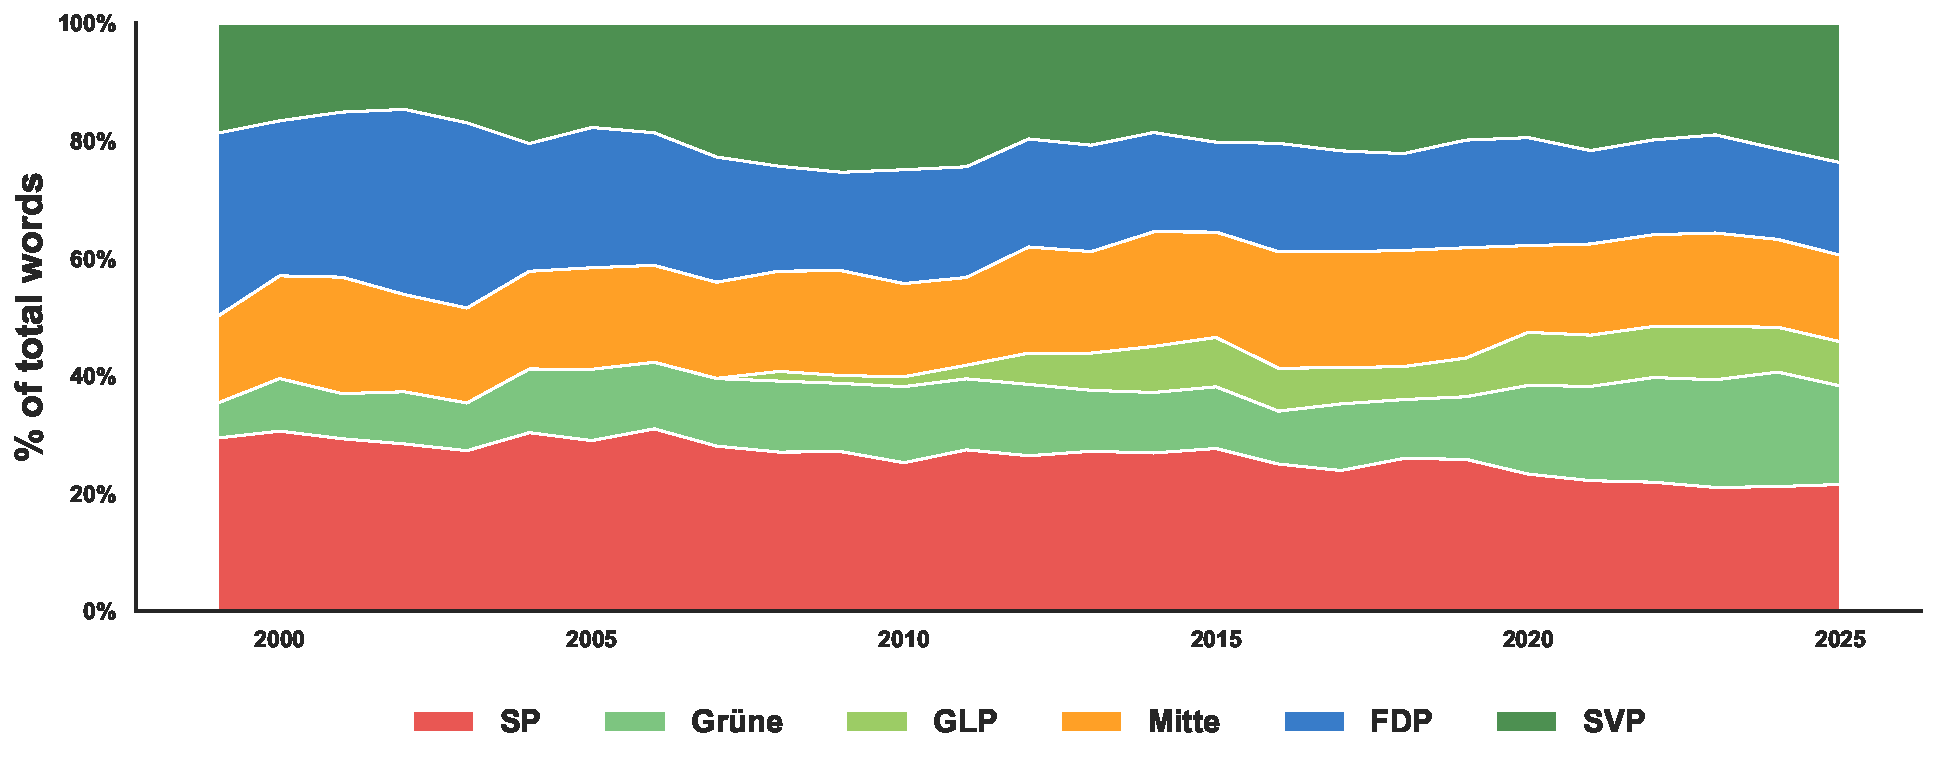
\includegraphics[width=0.92\textwidth,height=0.82\textheight,keepaspectratio]{desc_06_floor_time_share.pdf}
    \end{frame}
\begin{frame}{Topic Distribution Over Time --- Nationalrat}
    \centering
    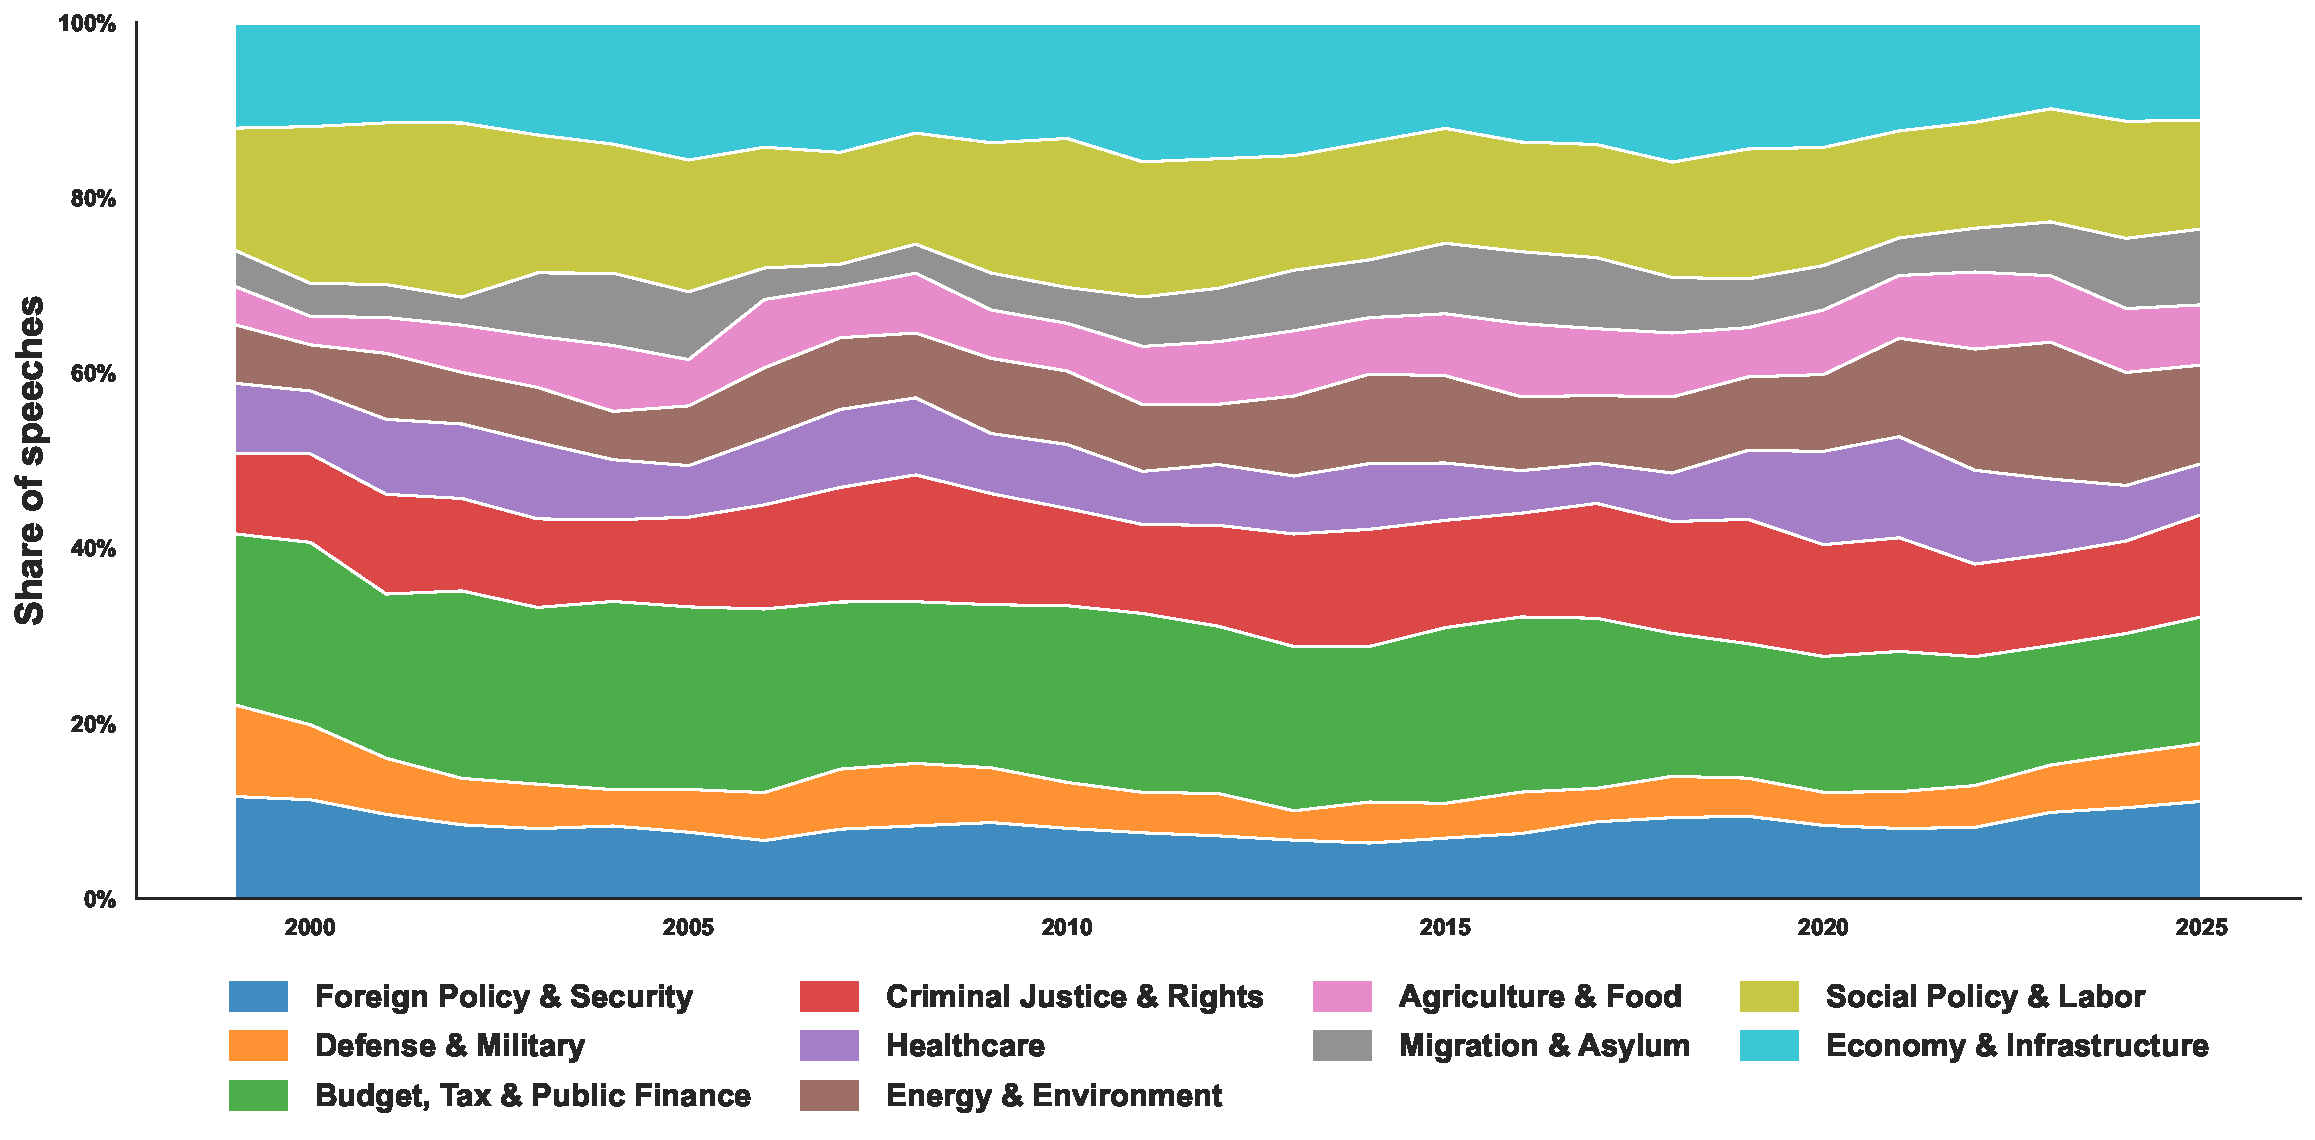
\includegraphics[width=0.97\textwidth,height=0.82\textheight,keepaspectratio]{nationalrat_fig_parlacap_broad_topic_stacked_smoothed.pdf}
    \end{frame}
\begin{frame}{Topic Emphasis by Party --- Nationalrat}
    \centering
    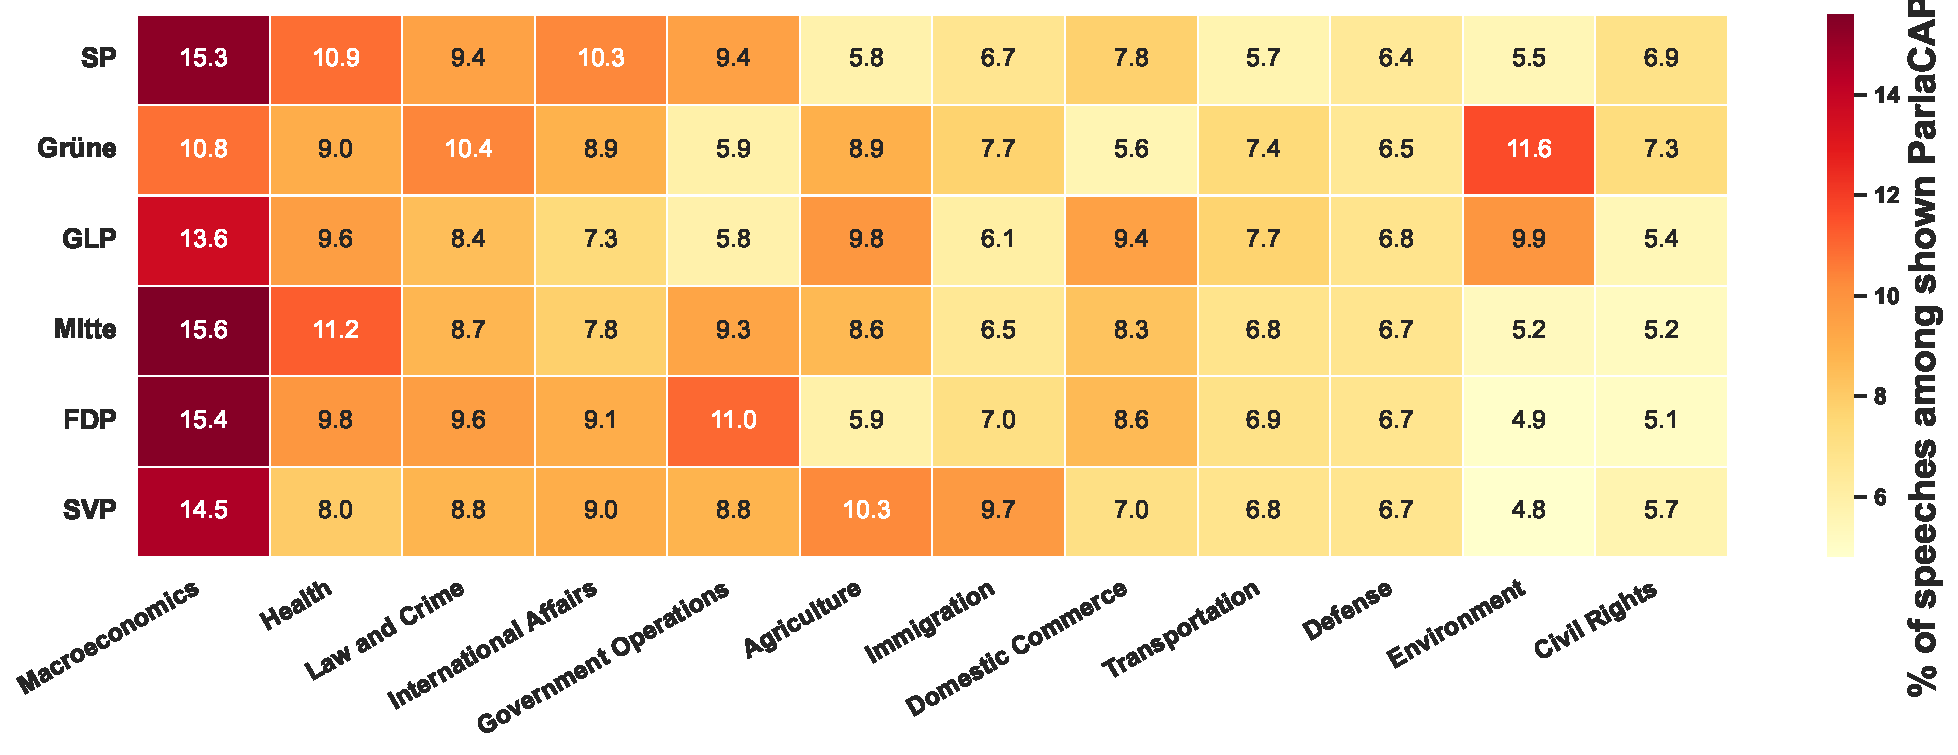
\includegraphics[width=0.94\textwidth,height=0.82\textheight,keepaspectratio]{fig_v4_topic_merged_party_noproc.pdf}
    \end{frame}
\begin{frame}{Absolute Shift in Parliamentary Attention --- Nationalrat}
    \centering
    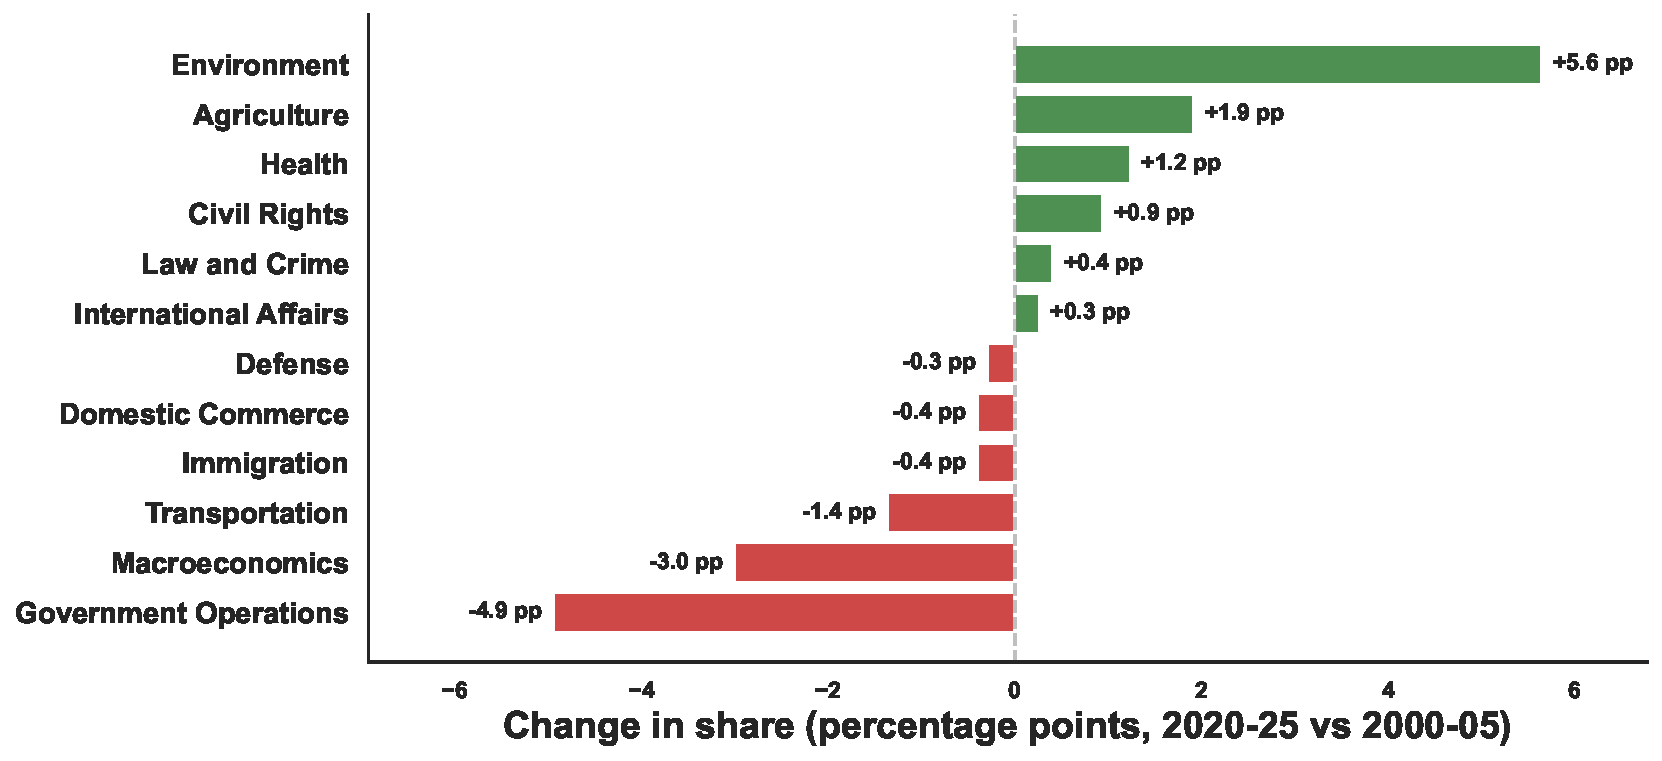
\includegraphics[width=0.82\textwidth,height=0.82\textheight,keepaspectratio]{fig_lt_topic_shift_noproc.pdf}
    \end{frame}
\begin{frame}{Relative Shift in Parliamentary Attention --- Nationalrat}
    \centering
    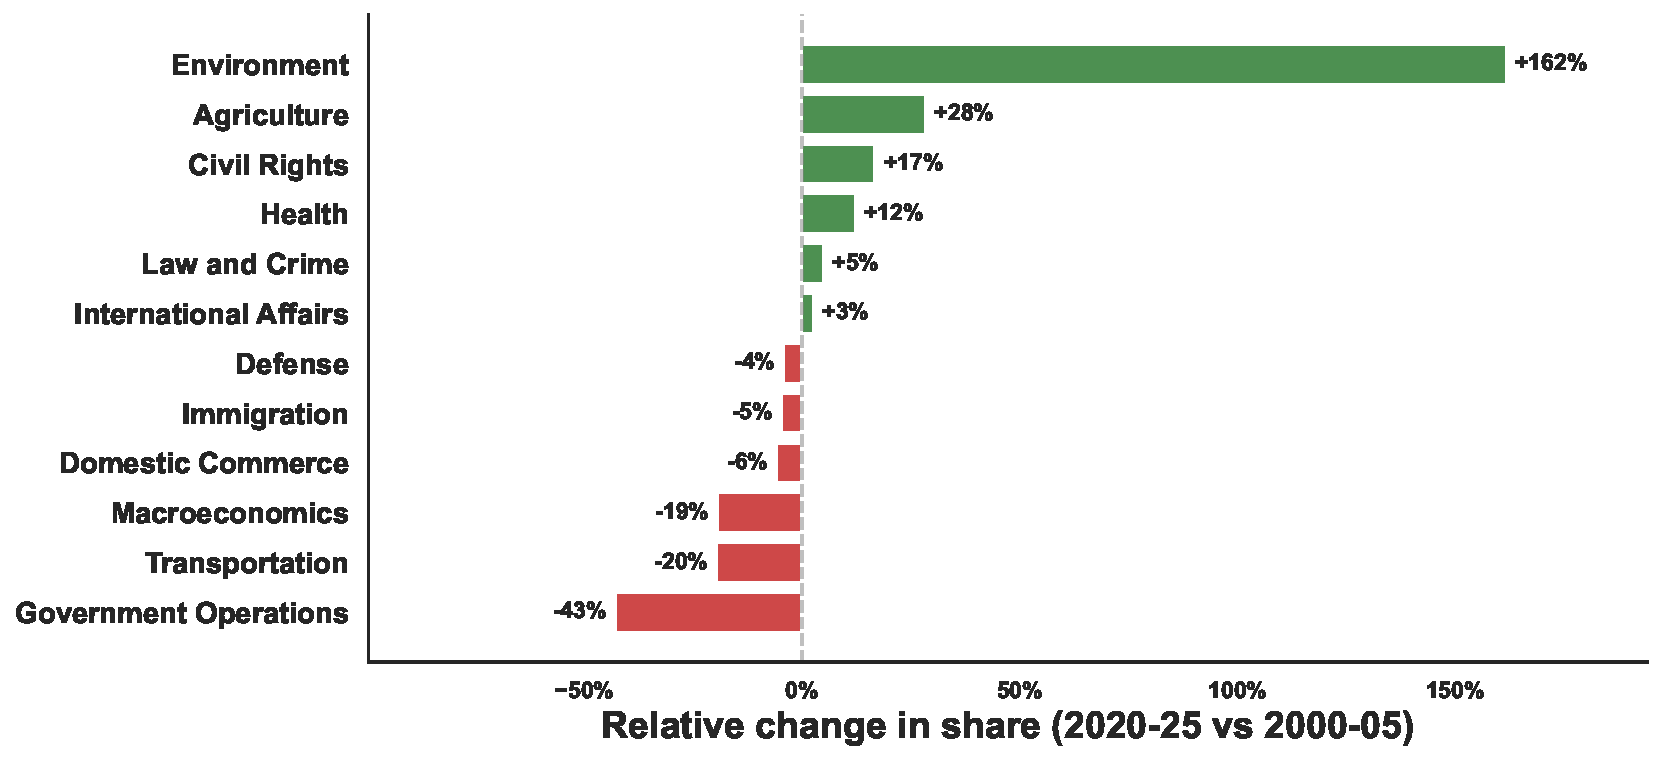
\includegraphics[width=0.82\textwidth,height=0.82\textheight,keepaspectratio]{fig_lt_topic_shift_proportion.pdf}
    \end{frame}
\begin{frame}{Who Drives Topic Shifts? --- Nationalrat}
    \centering
    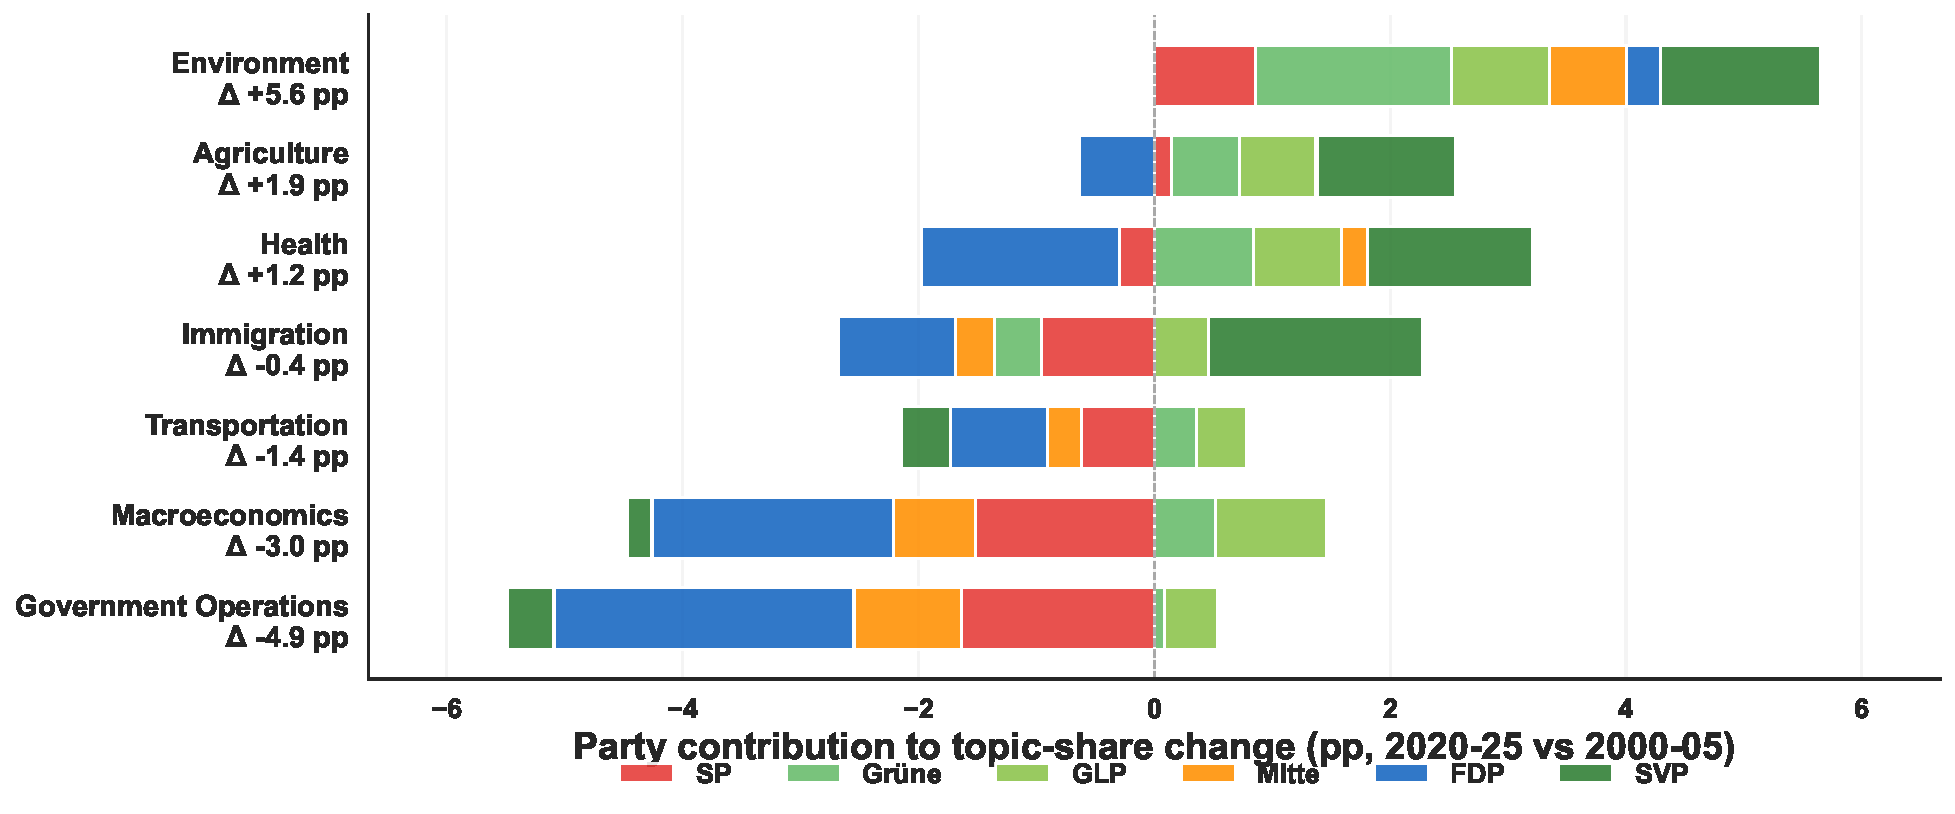
\includegraphics[width=0.88\textwidth,height=0.82\textheight,keepaspectratio]{nationalrat_fig_topic_shift_drivers_by_party.pdf}
    \end{frame}
\begin{frame}{Emotional Rhetoric --- Nationalrat}
    \centering
    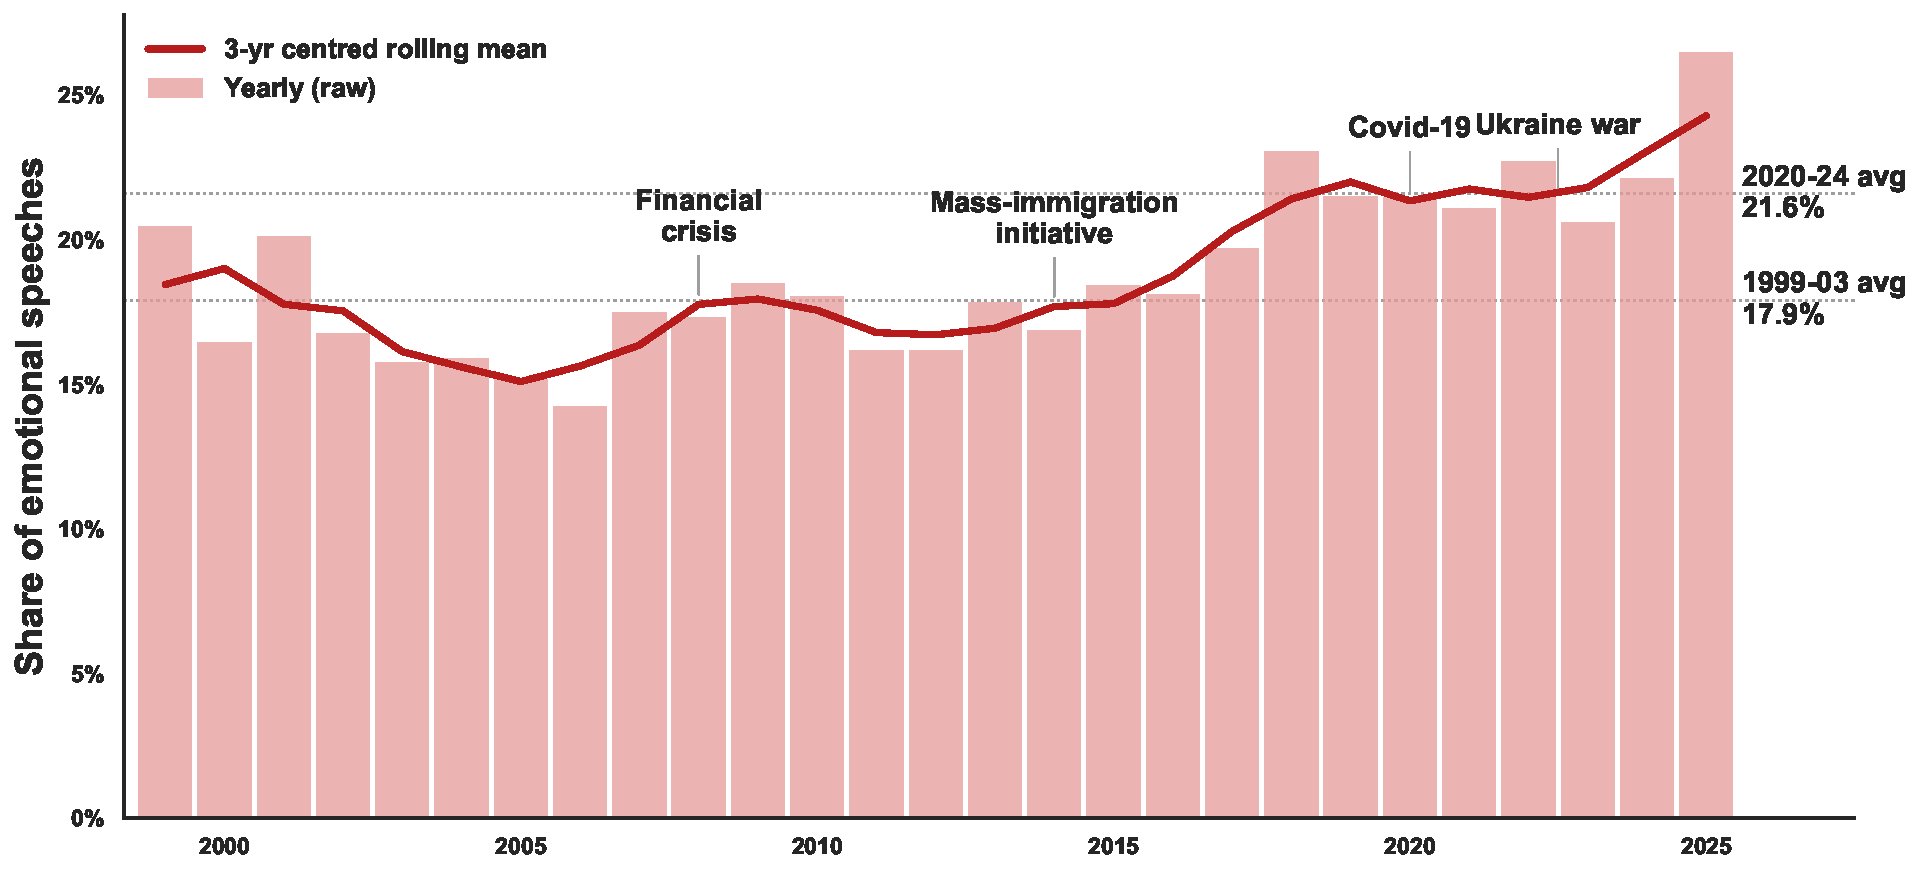
\includegraphics[width=0.92\textwidth,height=0.82\textheight,keepaspectratio]{fig_lt_defD_overall_time.pdf}
    \end{frame}
\begin{frame}{Emotional Rhetoric by Party --- Nationalrat}
    \centering
    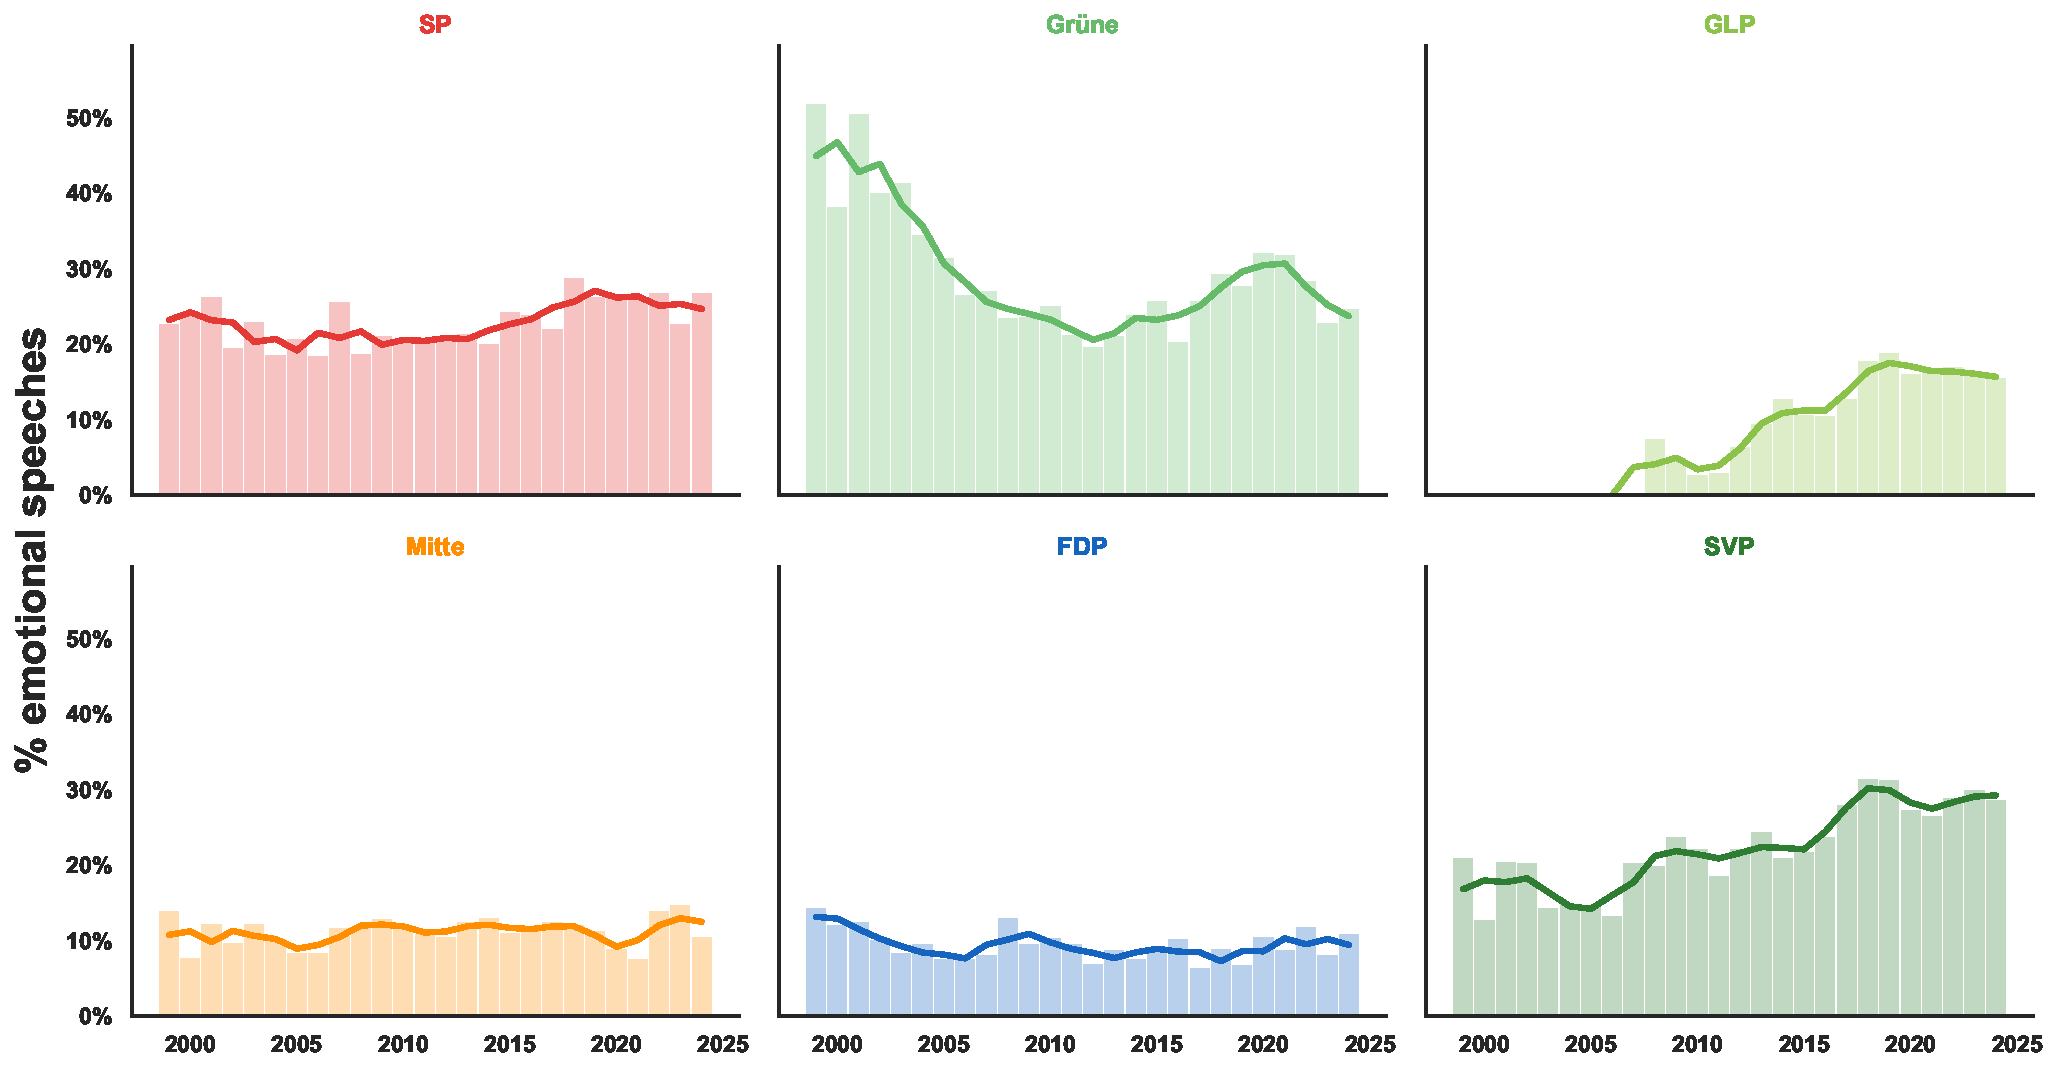
\includegraphics[width=0.92\textwidth,height=0.82\textheight,keepaspectratio]{fig_lt_defD_by_party.pdf}
    \end{frame}
\begin{frame}{Emotional Rhetoric by Legislature and Party --- Nationalrat}
\centering
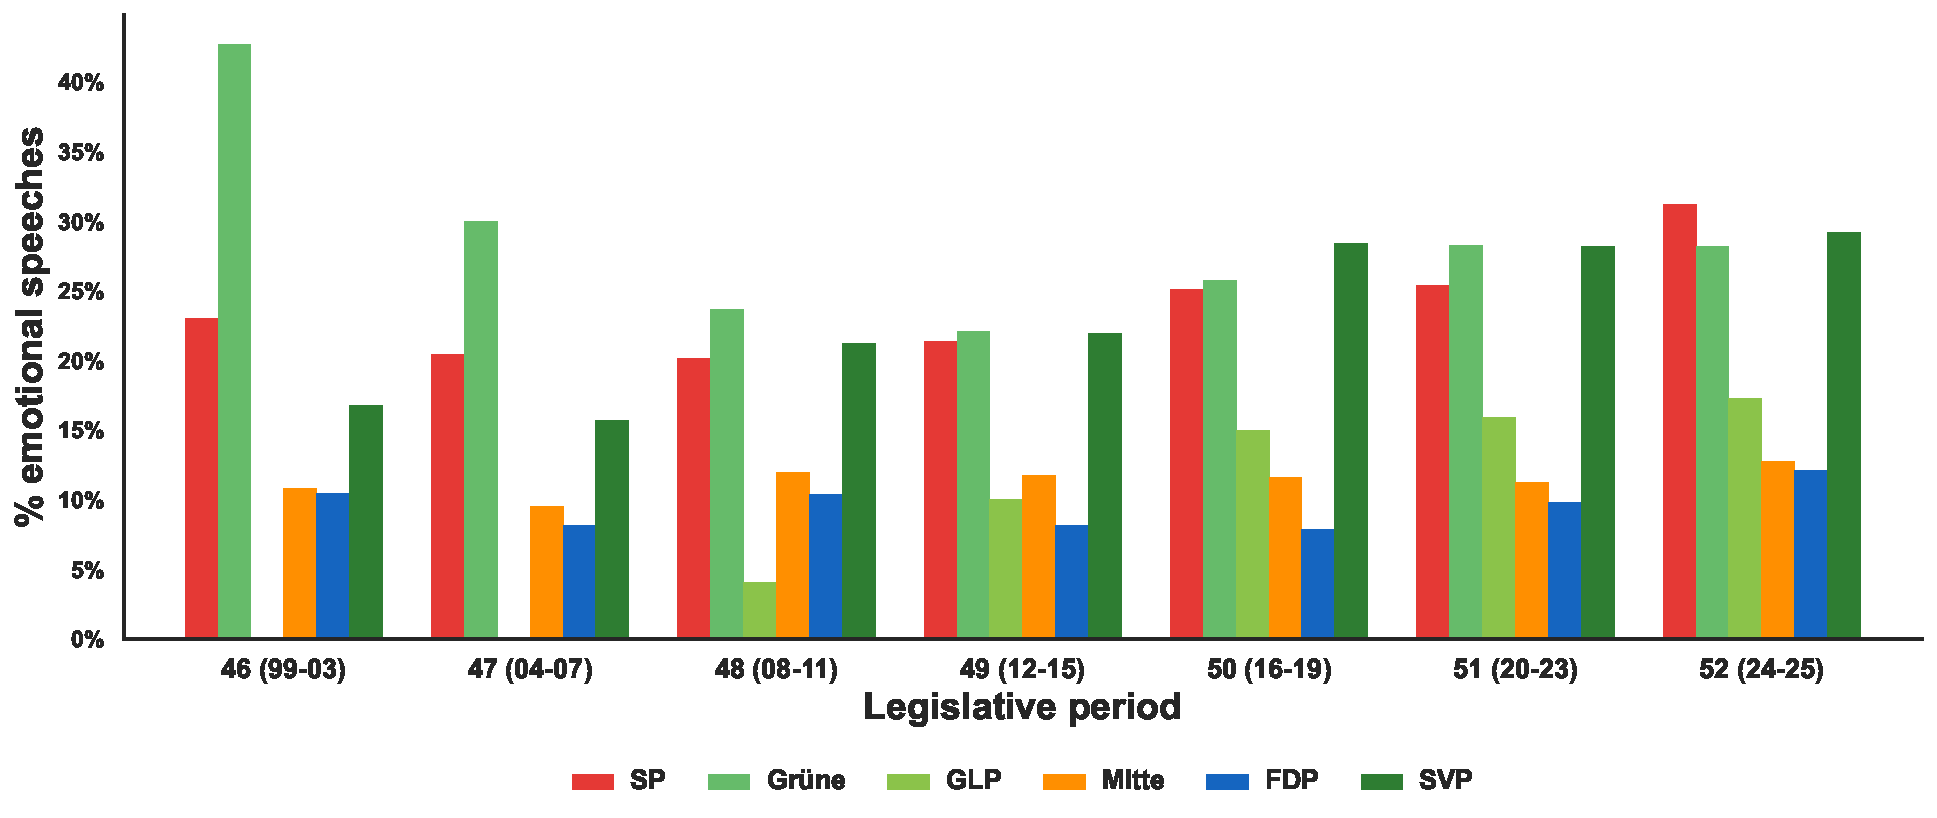
\includegraphics[width=0.93\textwidth,height=0.78\textheight,keepaspectratio]{fig_lt_defD_by_legislature.pdf}
\vfill
{\footnotesize\textit{Note:} Periods are split at federal National Council election dates (October; first sittings of the new parliament are from that election onward). GLP (PVL) entered with the 2007 election (48th period), so there is no 47th-period bar for GLP.}
\end{frame}
\begin{frame}{Emotional Rhetoric Score --- Nationalrat}
    \centering
    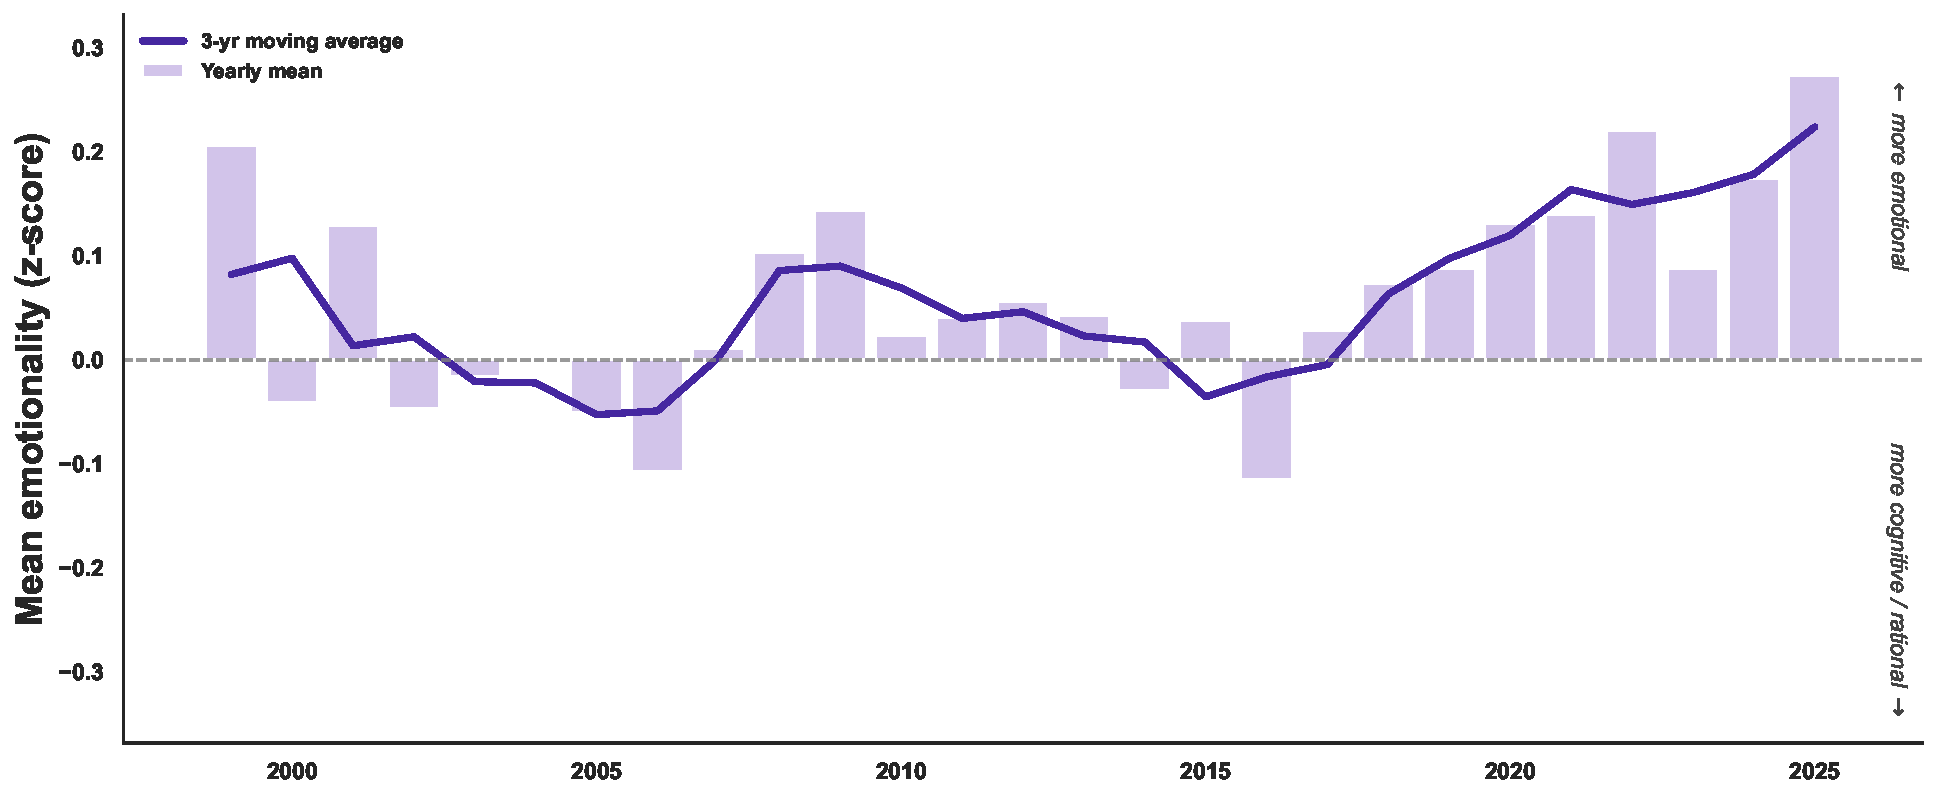
\includegraphics[width=0.90\textwidth,height=0.82\textheight,keepaspectratio]{nationalrat_fig_lt_ga_emotionality_time.pdf}
    \end{frame}
\begin{frame}{Emotional Rhetoric Score by Party --- Nationalrat}
    \centering
    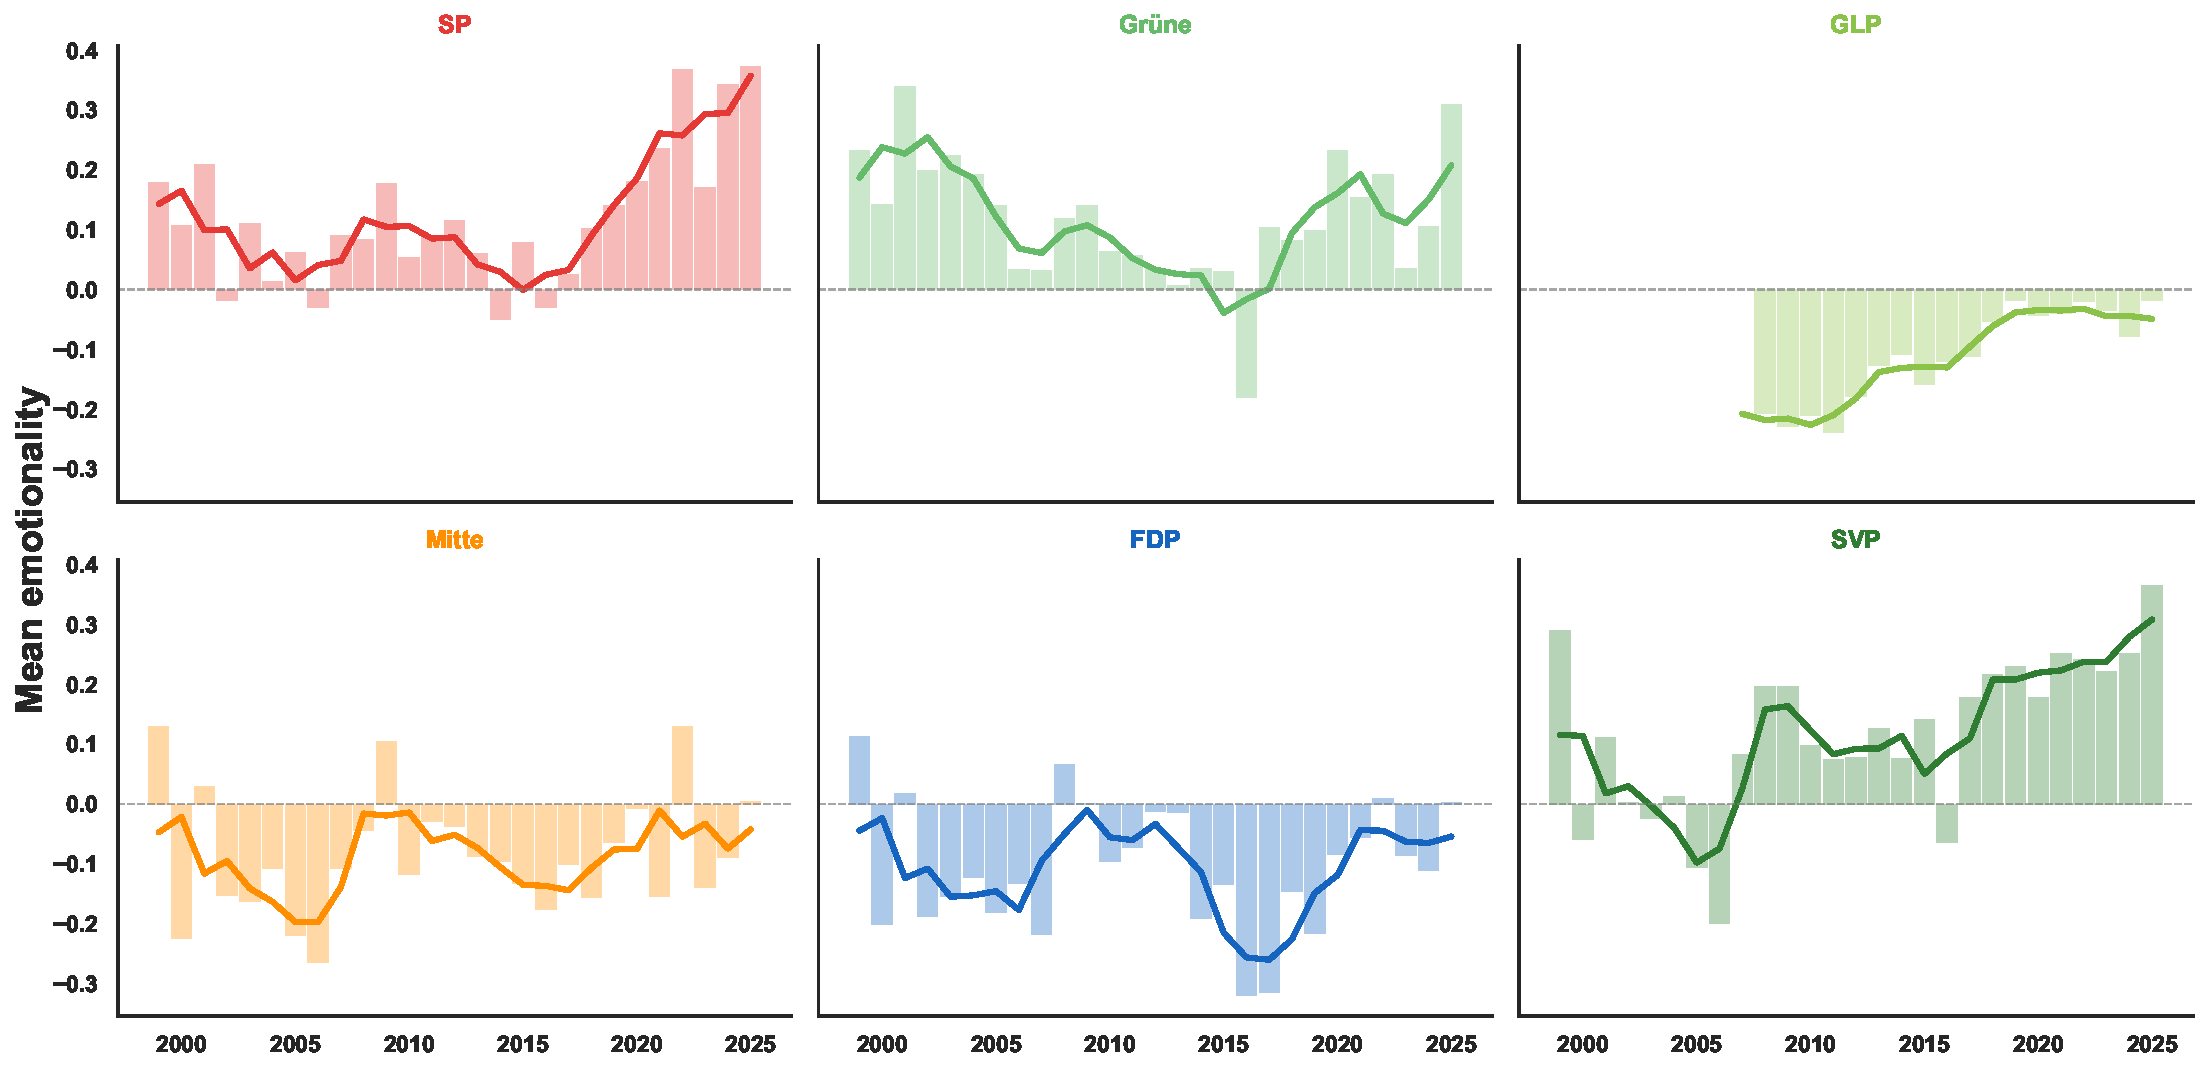
\includegraphics[width=0.92\textwidth,height=0.82\textheight,keepaspectratio]{nationalrat_fig_lt_ga_emotionality_party_facet.pdf}
    \end{frame}
\begin{frame}{Emotional Rhetoric Baseline Index --- Nationalrat}
    \centering
    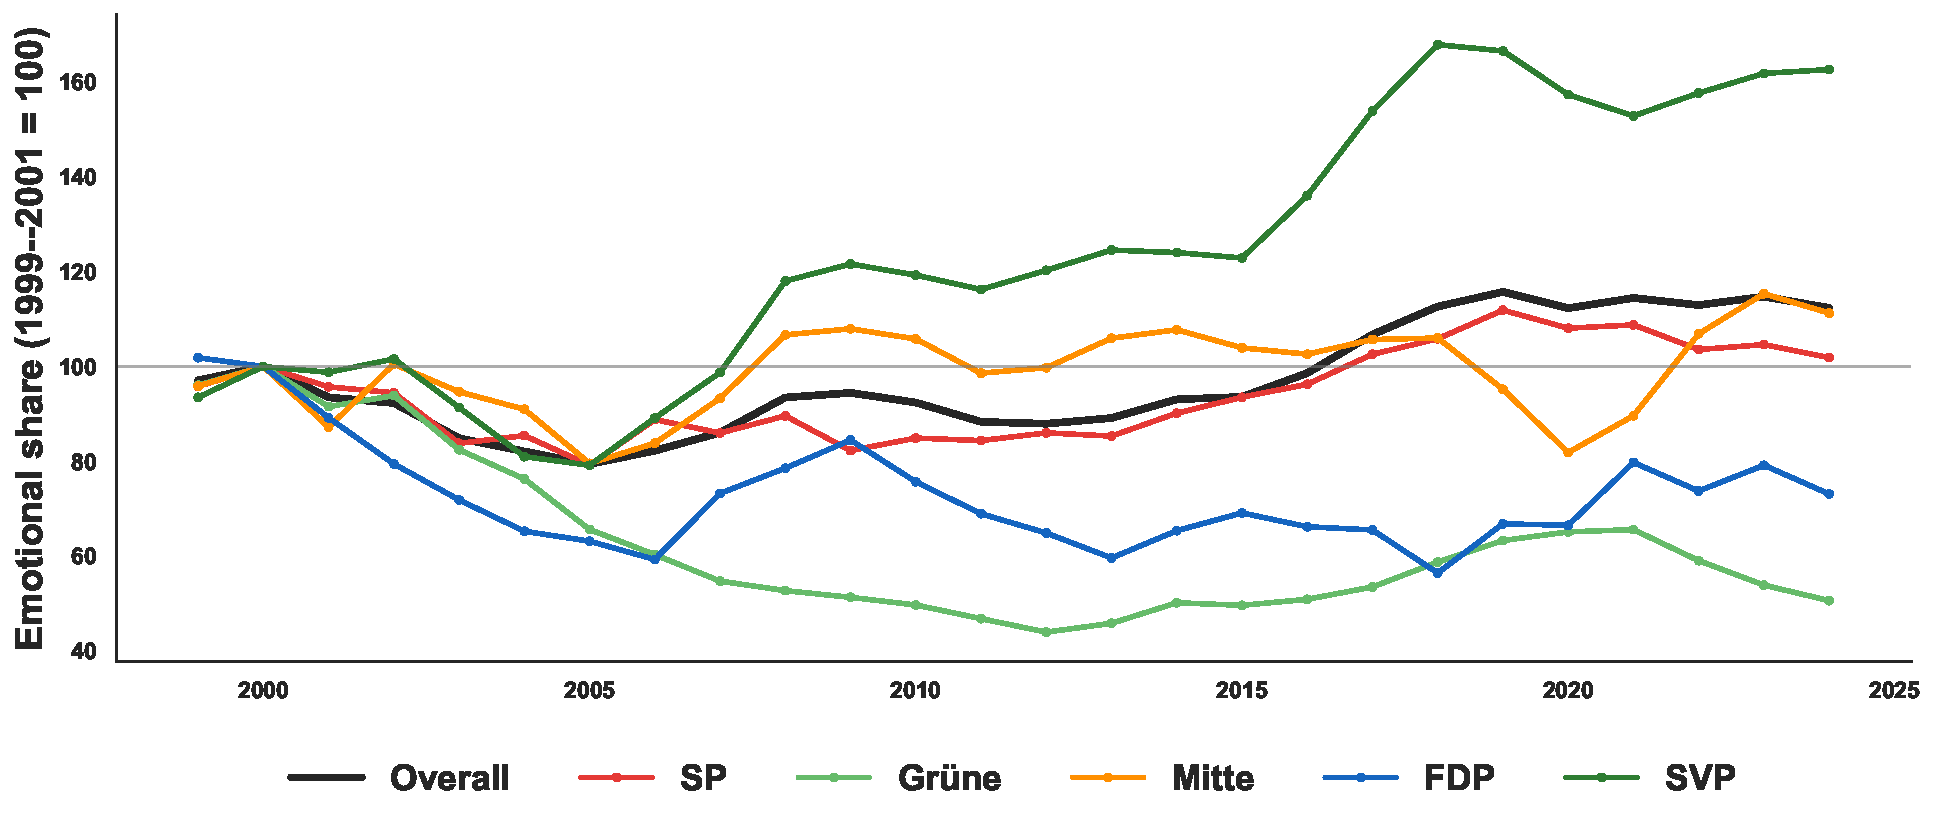
\includegraphics[width=0.86\textwidth,height=0.82\textheight,keepaspectratio]{fig_lt_llm_emo_index100.pdf}
    \end{frame}
\begin{frame}{Dominant Emotion in Emotional Speeches --- Nationalrat}
    \centering
    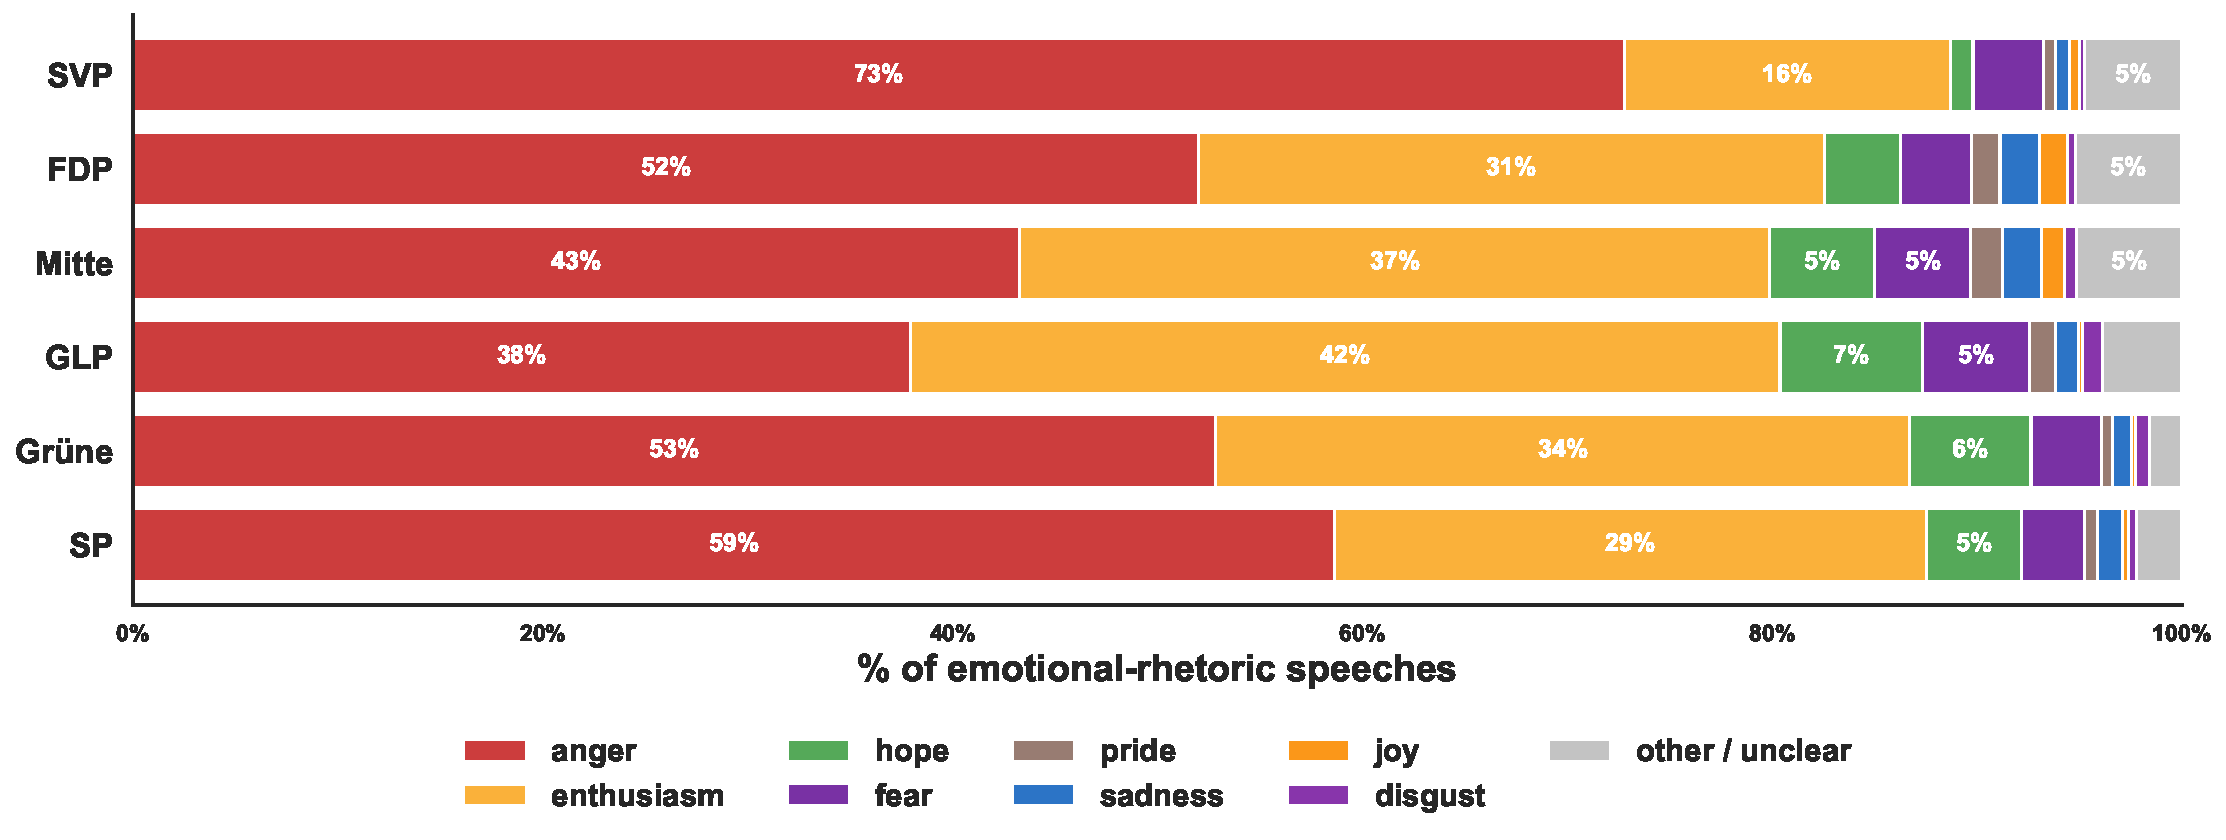
\includegraphics[width=0.92\textwidth,height=0.82\textheight,keepaspectratio]{fig_lt_llm_dominant_party.pdf}
    \end{frame}
\begin{frame}{Enthusiasm, Anger, Hope, Fear by Party --- Nationalrat}
\centering
\vfill
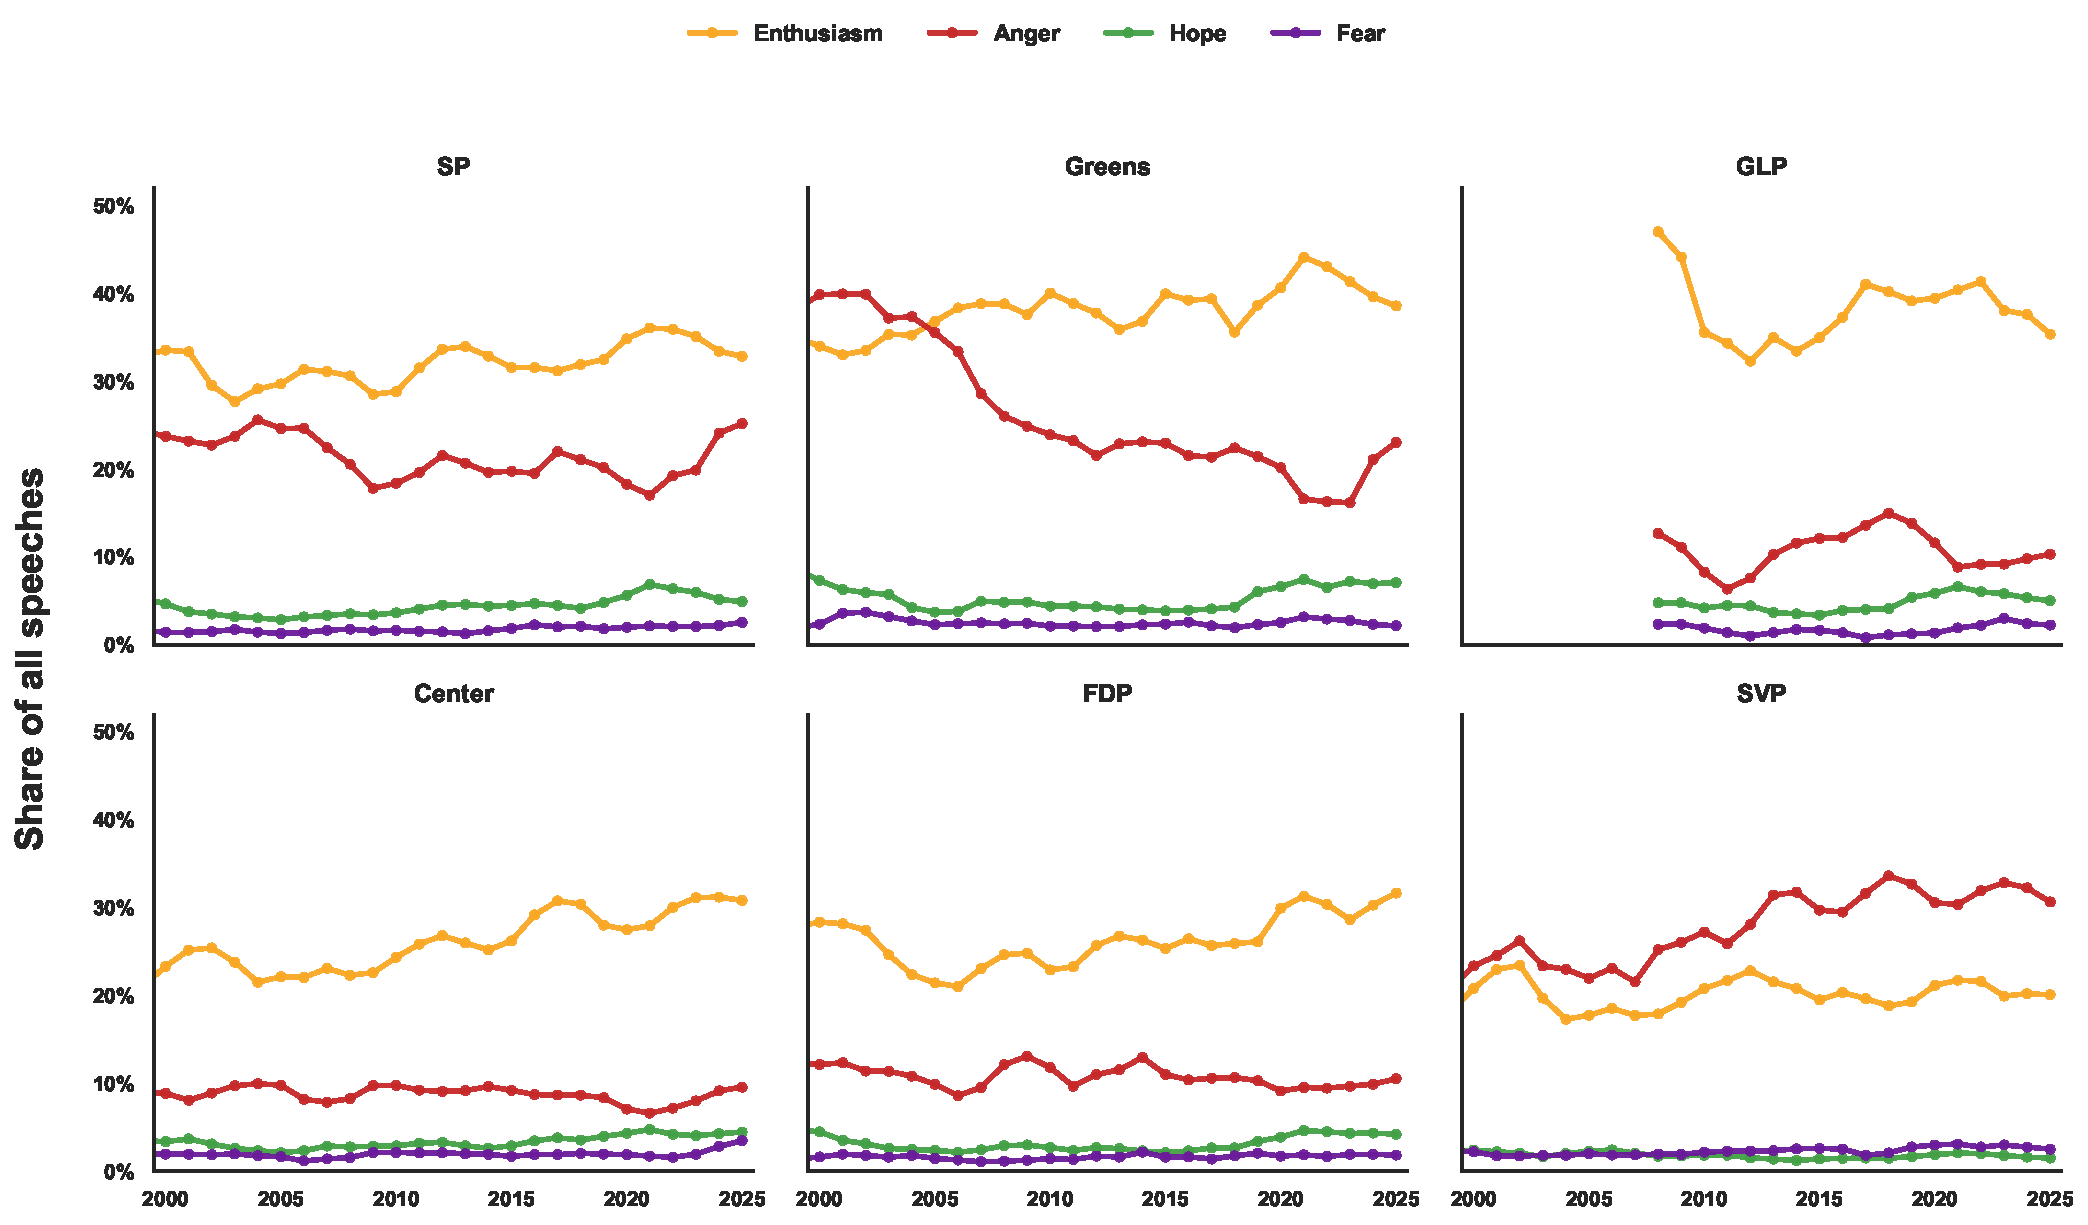
\includegraphics[width=0.99\textwidth,height=0.82\textheight,keepaspectratio]{emotions_ahef_over_time_by_party_from_csv.pdf}
\vfill
\end{frame}
\begin{frame}{Emotional Rhetoric by Topic --- Nationalrat}
    \centering
    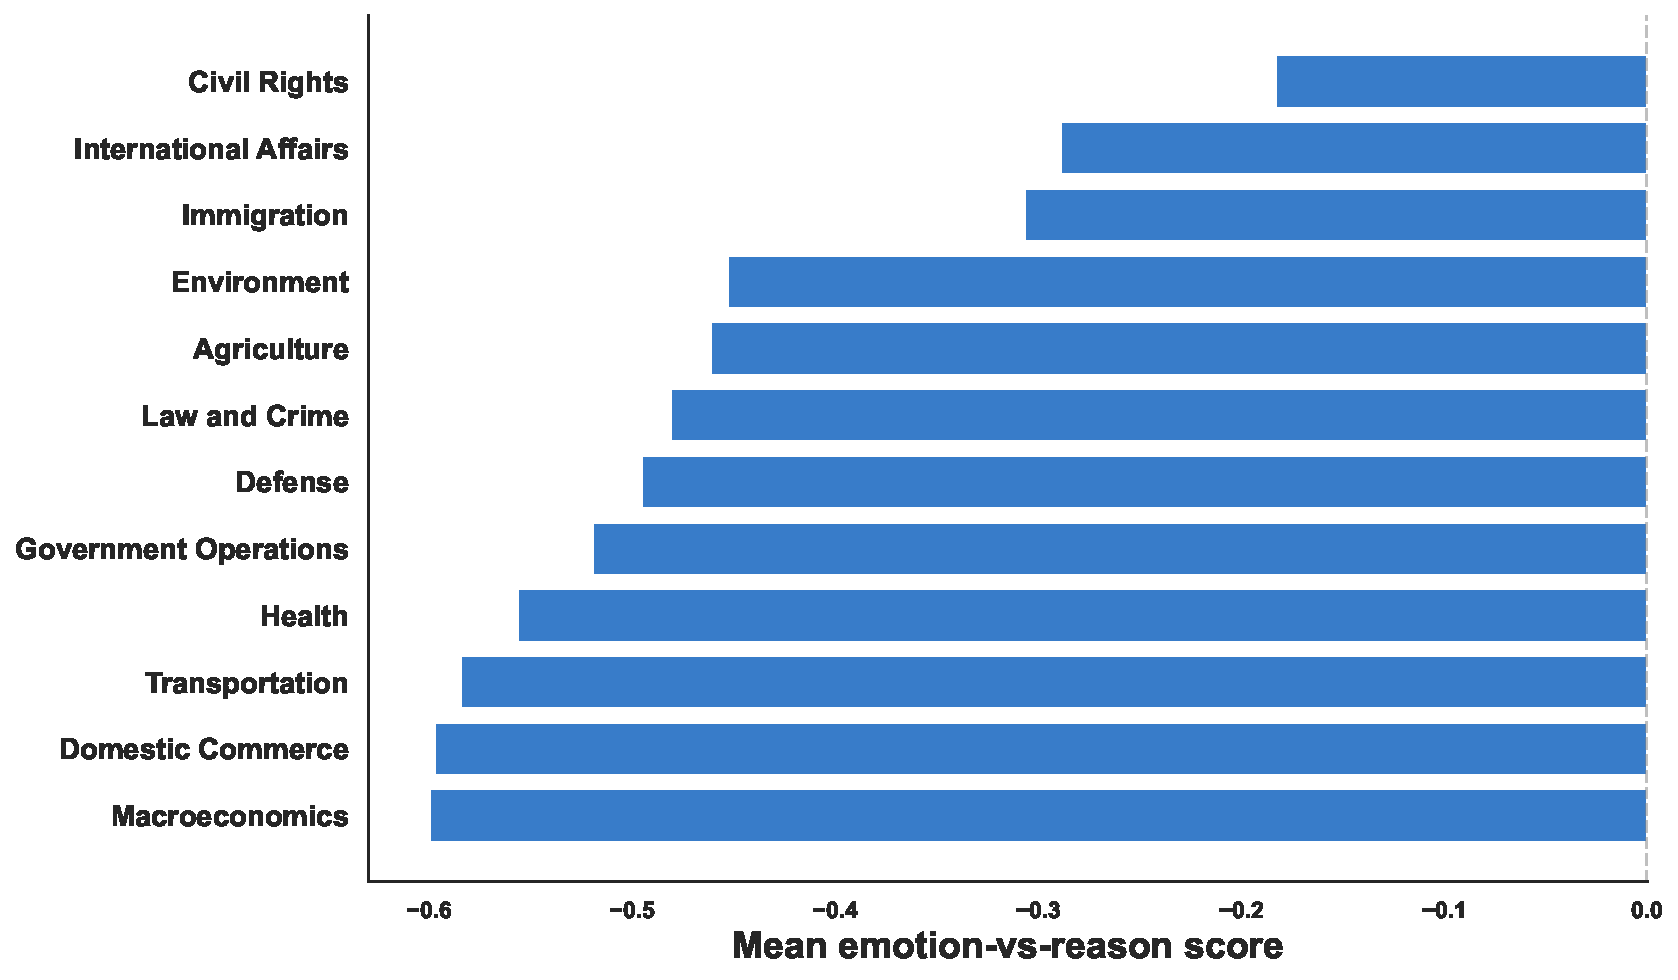
\includegraphics[width=0.78\textwidth,height=0.82\textheight,keepaspectratio]{fig_lt_emotionality_topic_large.pdf}
    \end{frame}
\begin{frame}{Emotional Rhetoric Gap by Topic (SVP vs SP) --- Nationalrat}
    \centering
    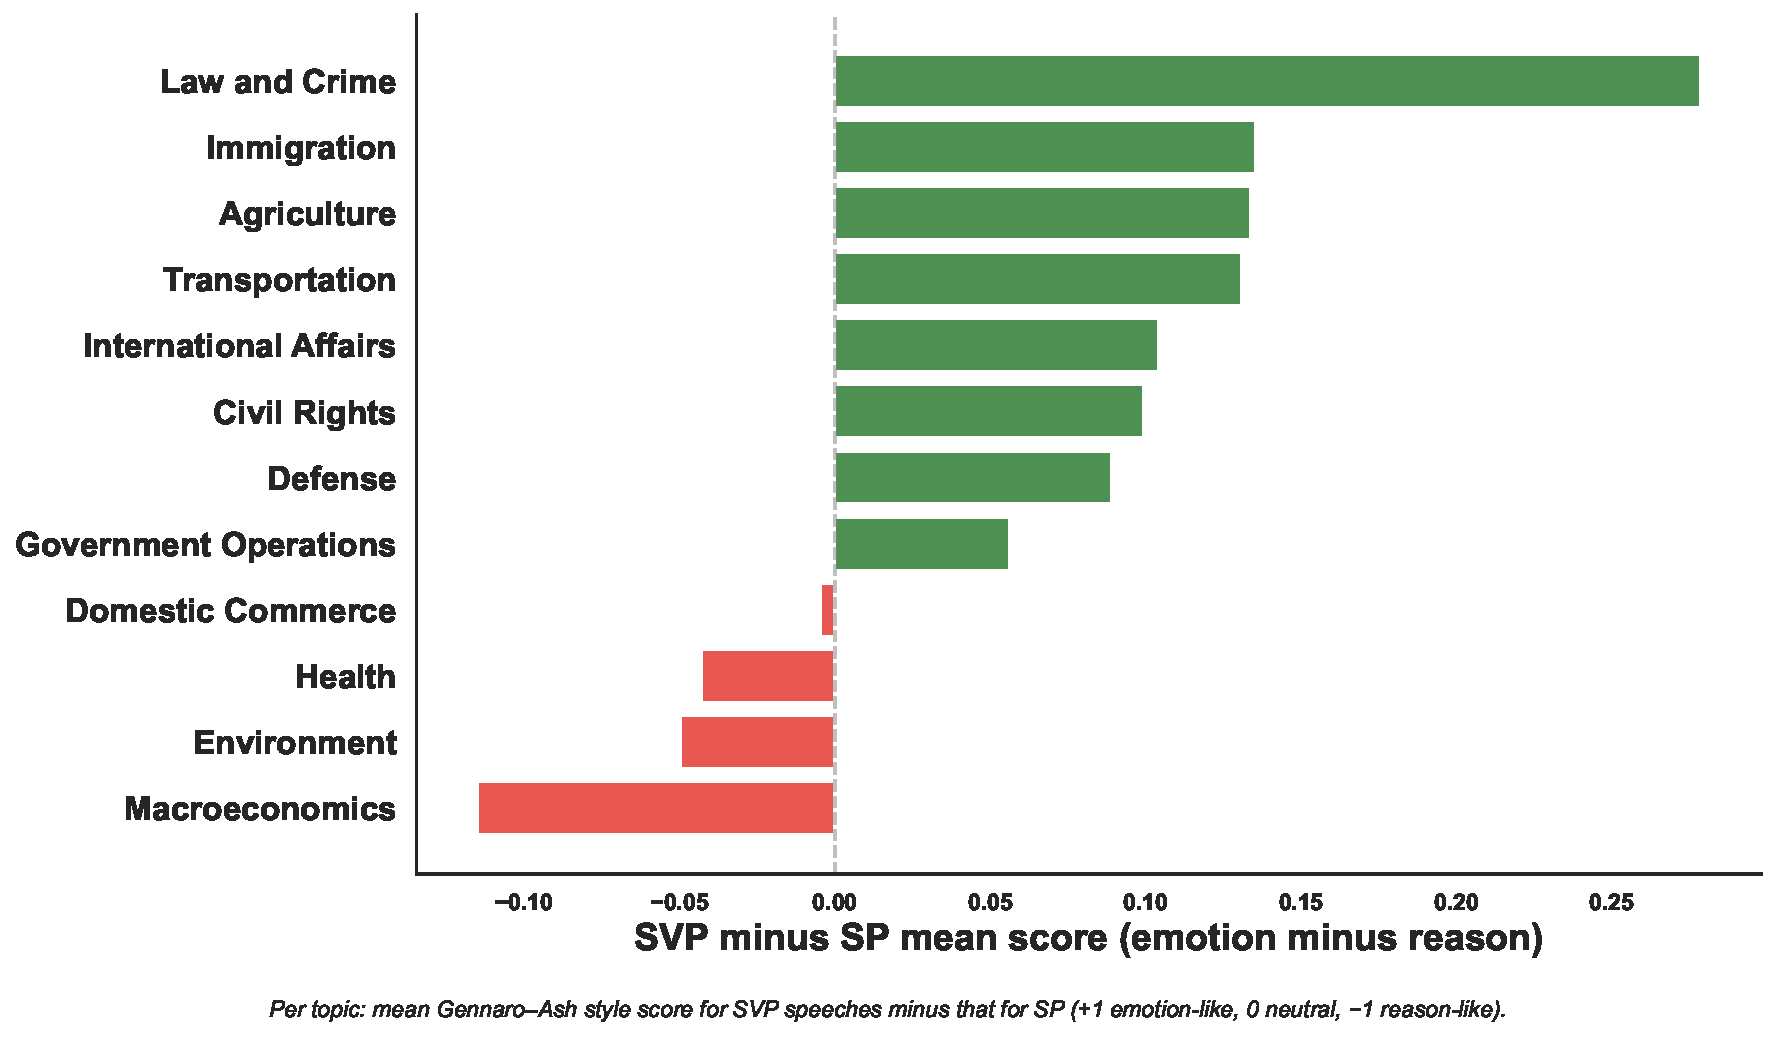
\includegraphics[width=0.72\textwidth,height=0.82\textheight,keepaspectratio]{fig_GA_party_ratio_by_topic.pdf}
    \end{frame}
\begin{frame}{Emotional Rhetoric by Topic --- Shift --- Nationalrat}
    \centering
    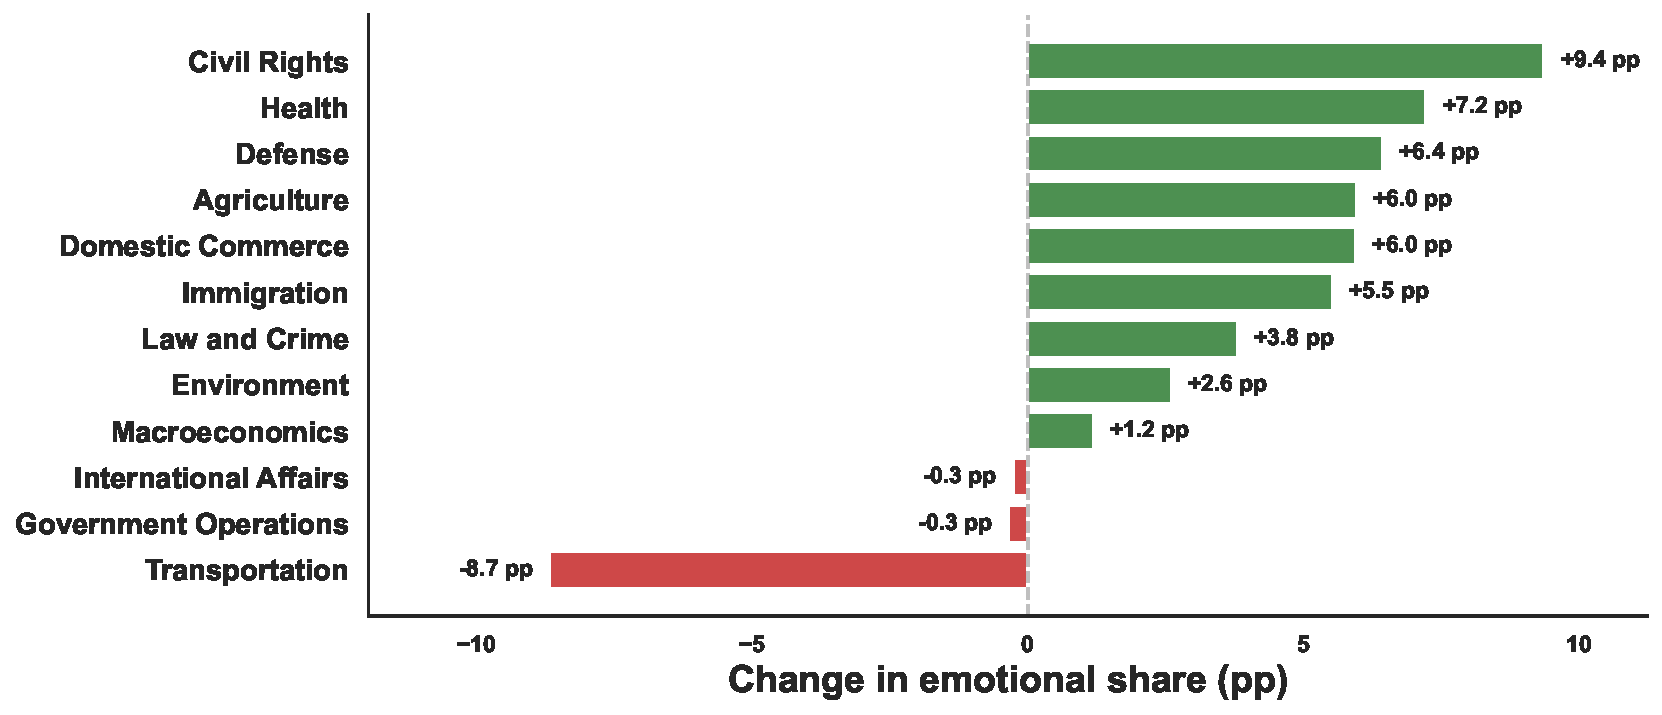
\includegraphics[width=0.80\textwidth,height=0.82\textheight,keepaspectratio]{fig_lt_defD_topic_shift.pdf}
    \end{frame}
\begin{frame}{Who Drives Emotional-Rhetoric Shifts Within Topics? --- Nationalrat}
\hypertarget{main.NR.emotion.drivers}{}
\centering
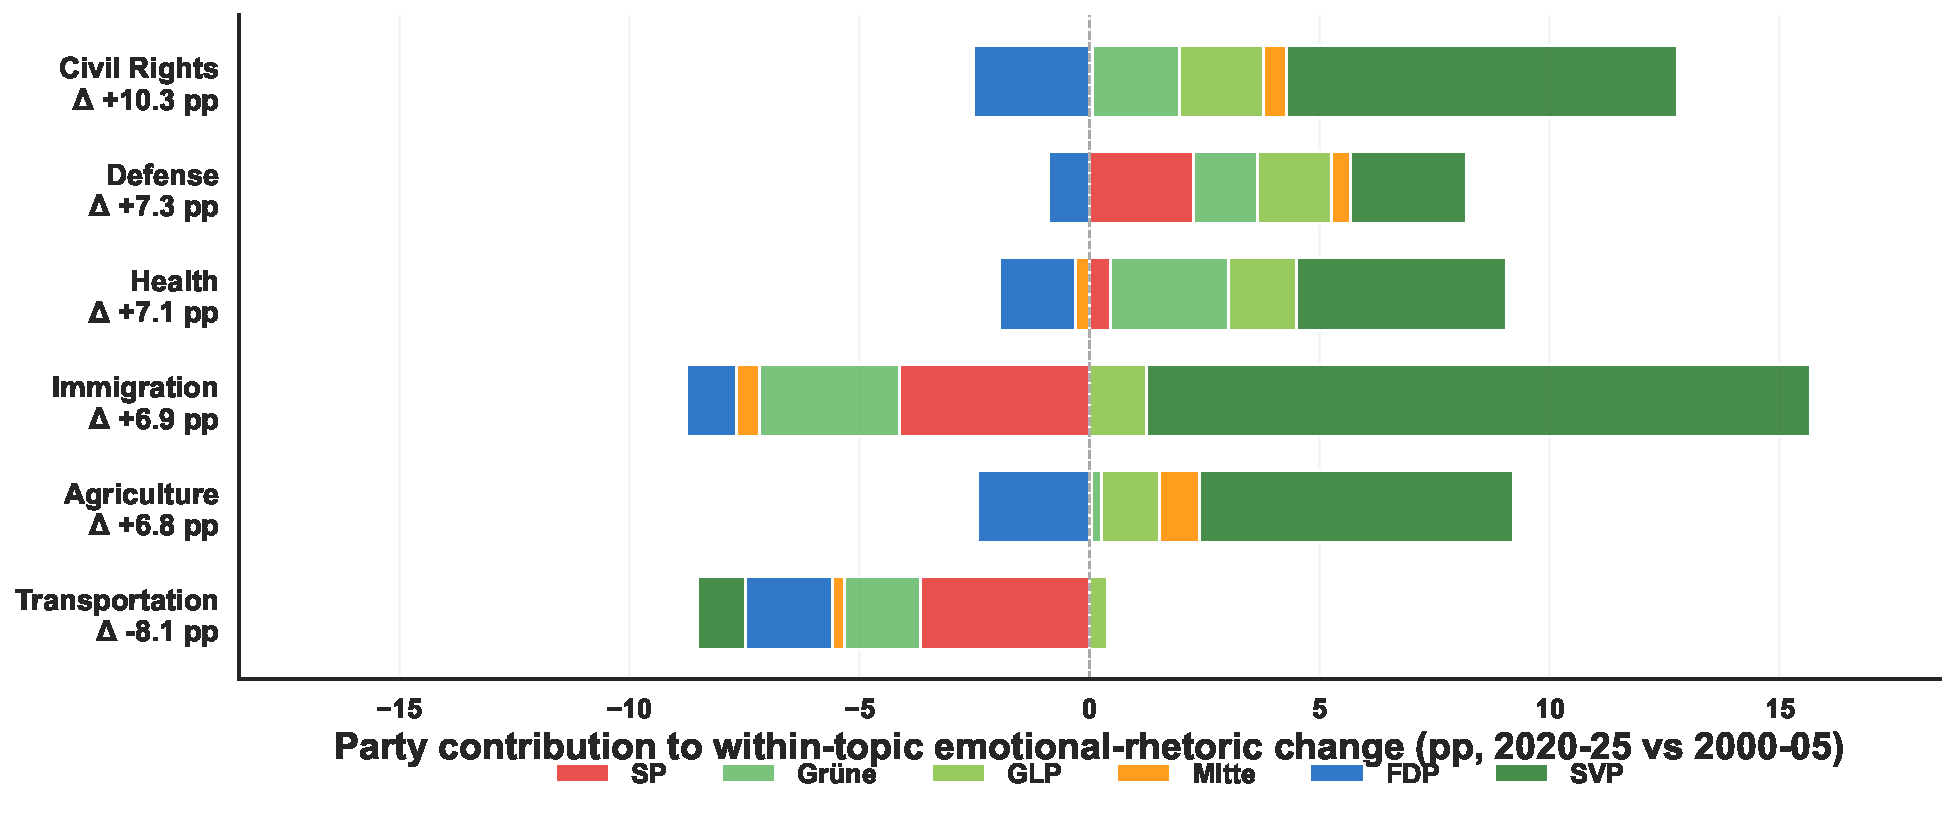
\includegraphics[width=0.88\textwidth,height=0.76\textheight,keepaspectratio]{nationalrat_fig_emotion_shift_within_topic_drivers_by_party.pdf}
\vfill
{\footnotesize\hyperlink{app.NR.emotion.drivers.table}{Appendix: tabular party contributions} (same decomposition in table form).}
\end{frame}
\begin{frame}{Emotional Rhetoric by Topic --- 2000--05 vs 2020--24 --- Nationalrat}
\centering
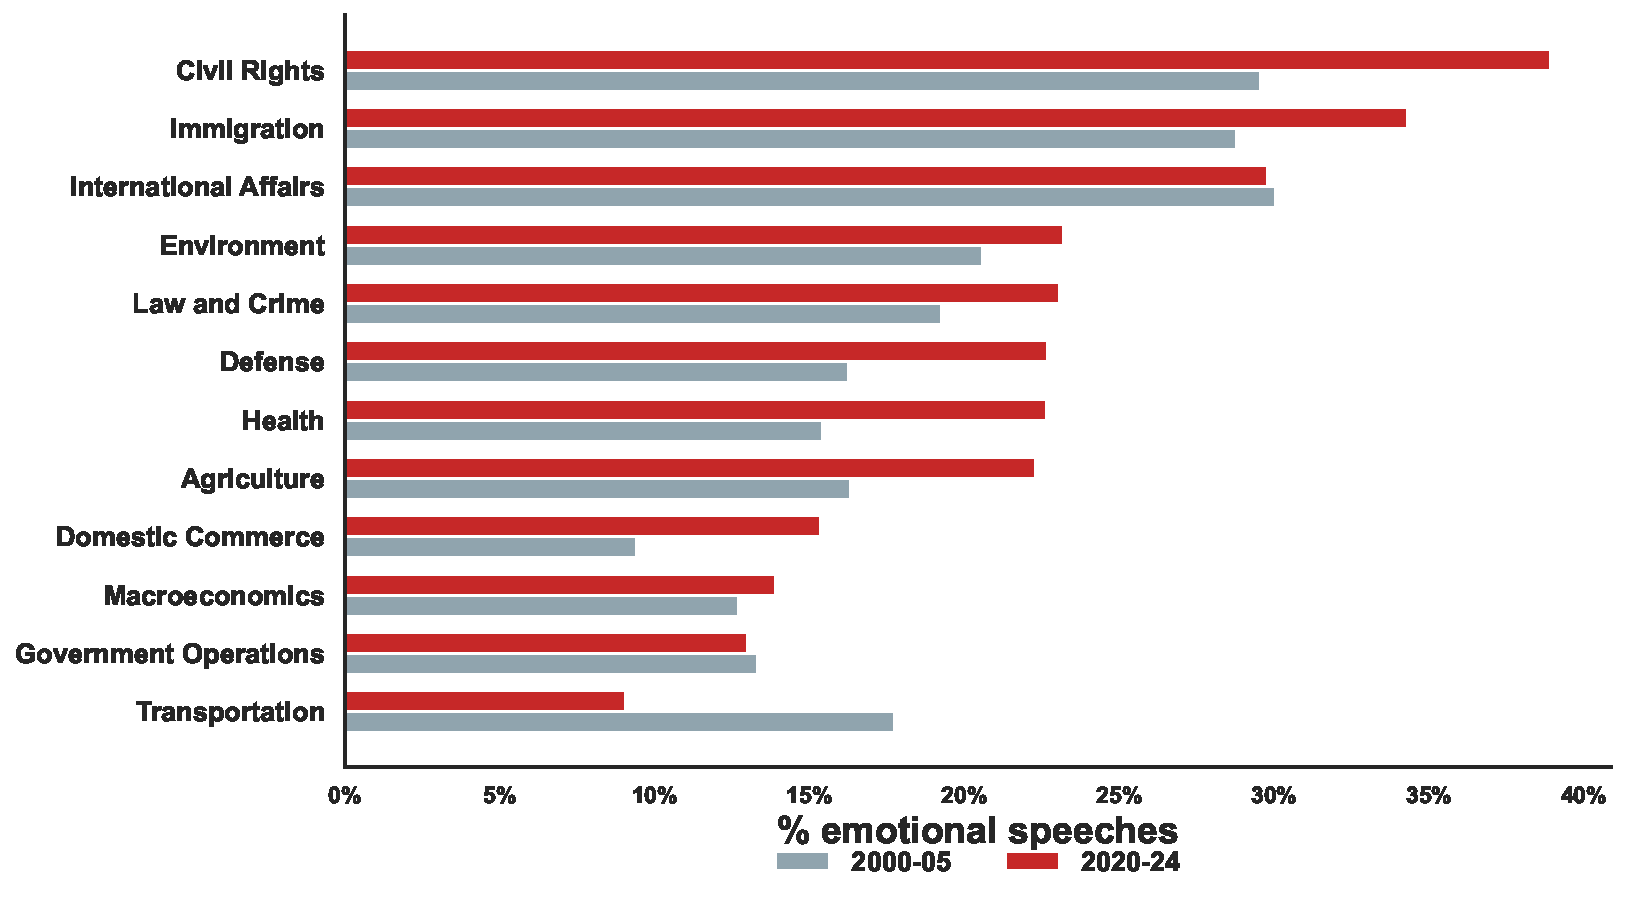
\includegraphics[width=0.86\textwidth,height=0.76\textheight,keepaspectratio]{fig_lt_defD_by_topic.pdf}
\vfill
{\footnotesize\textit{Note:} Topic bars pool all six parties; GLP (PVL) had only minimal National Council floor time in 2000--05, so the early window is driven mainly by the longer-established parties.}
\end{frame}
\begin{frame}{Gender Representation by Party --- Nationalrat}
    \centering
    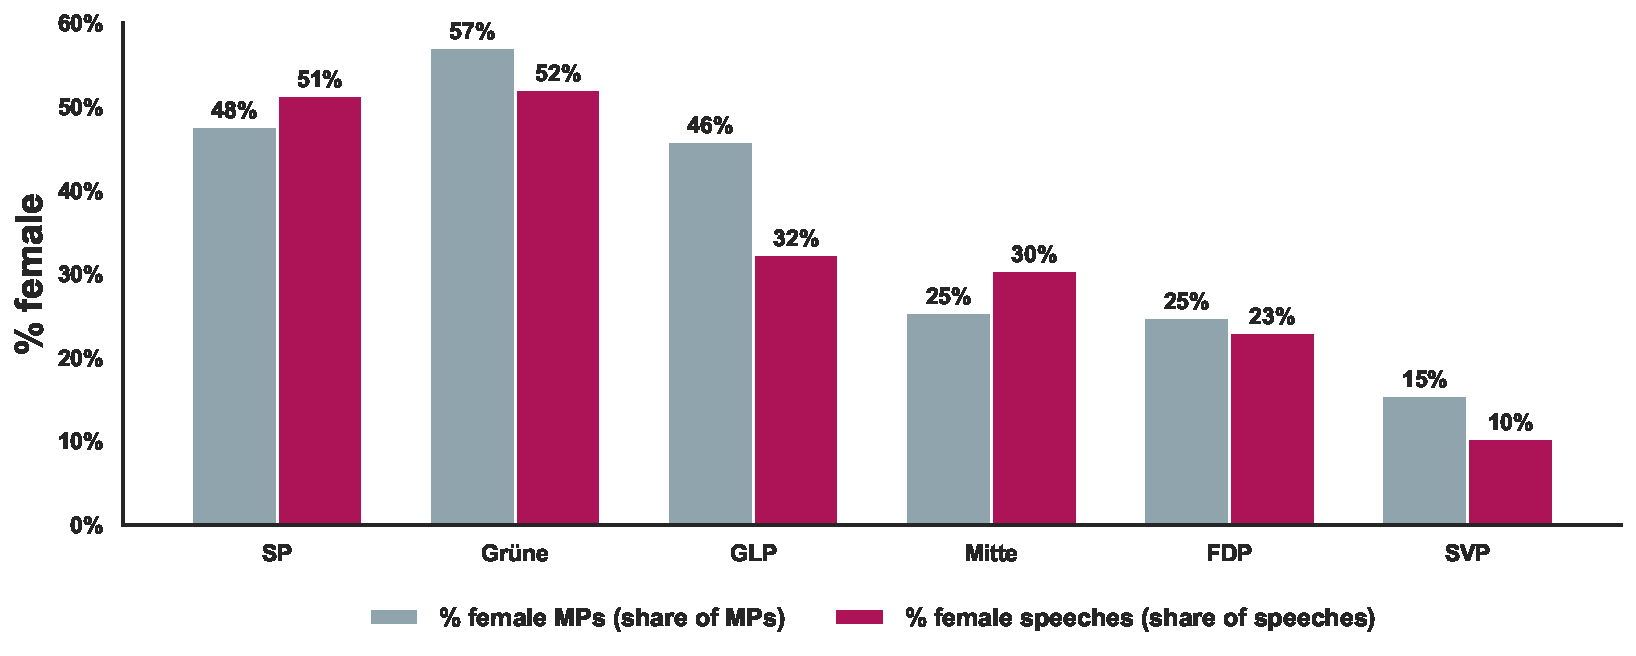
\includegraphics[width=0.82\textwidth,height=0.82\textheight,keepaspectratio]{fig_lt_gender_mp_vs_speeches_party.pdf}
    \end{frame}
\begin{frame}{Floor-Time Gap by Gender --- Nationalrat (1999--2025)}
    \centering
    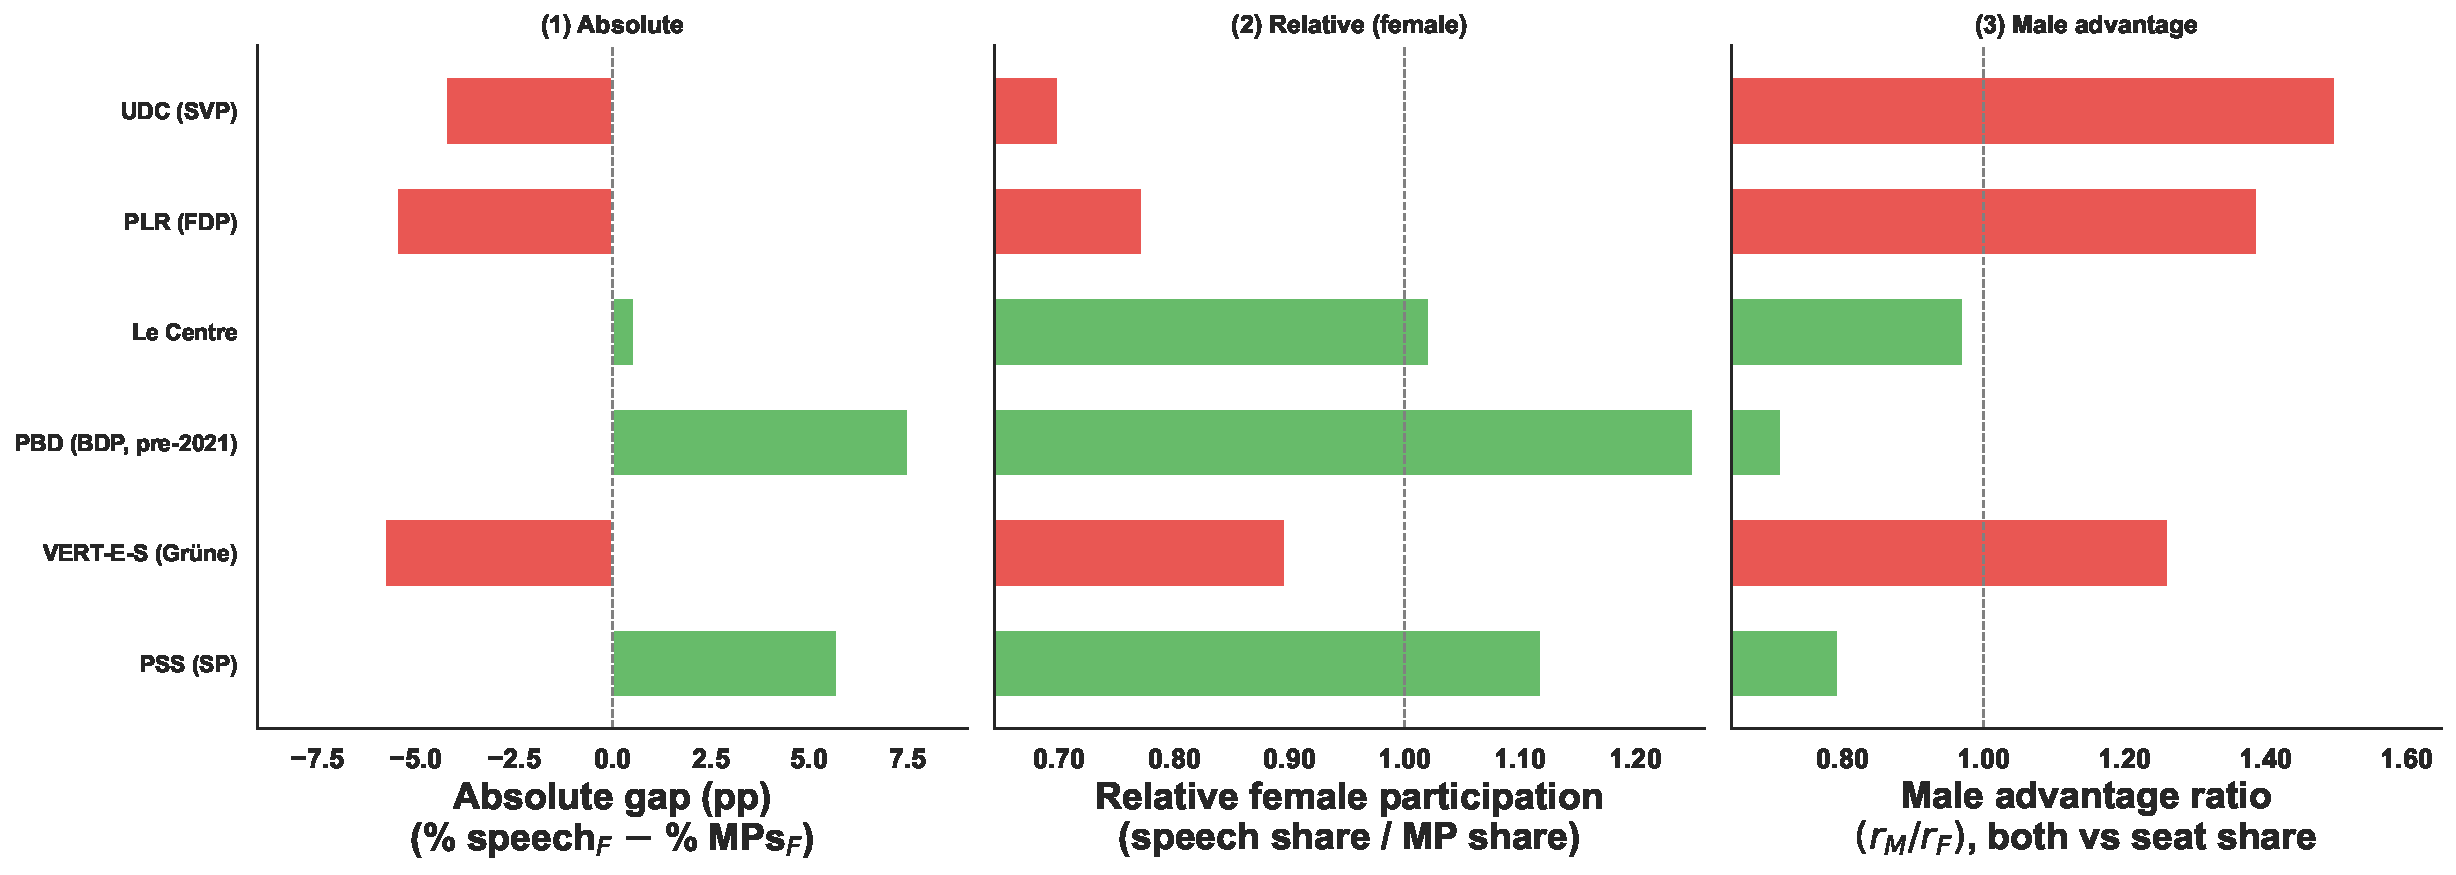
\includegraphics[width=0.95\textwidth,height=0.82\textheight,keepaspectratio]{fig_lt_gender_metrics_bars_1999_2025_nationalrat.pdf}
    \end{frame}
\begin{frame}{Canton Share of Speeches --- Nationalrat}
    \centering
    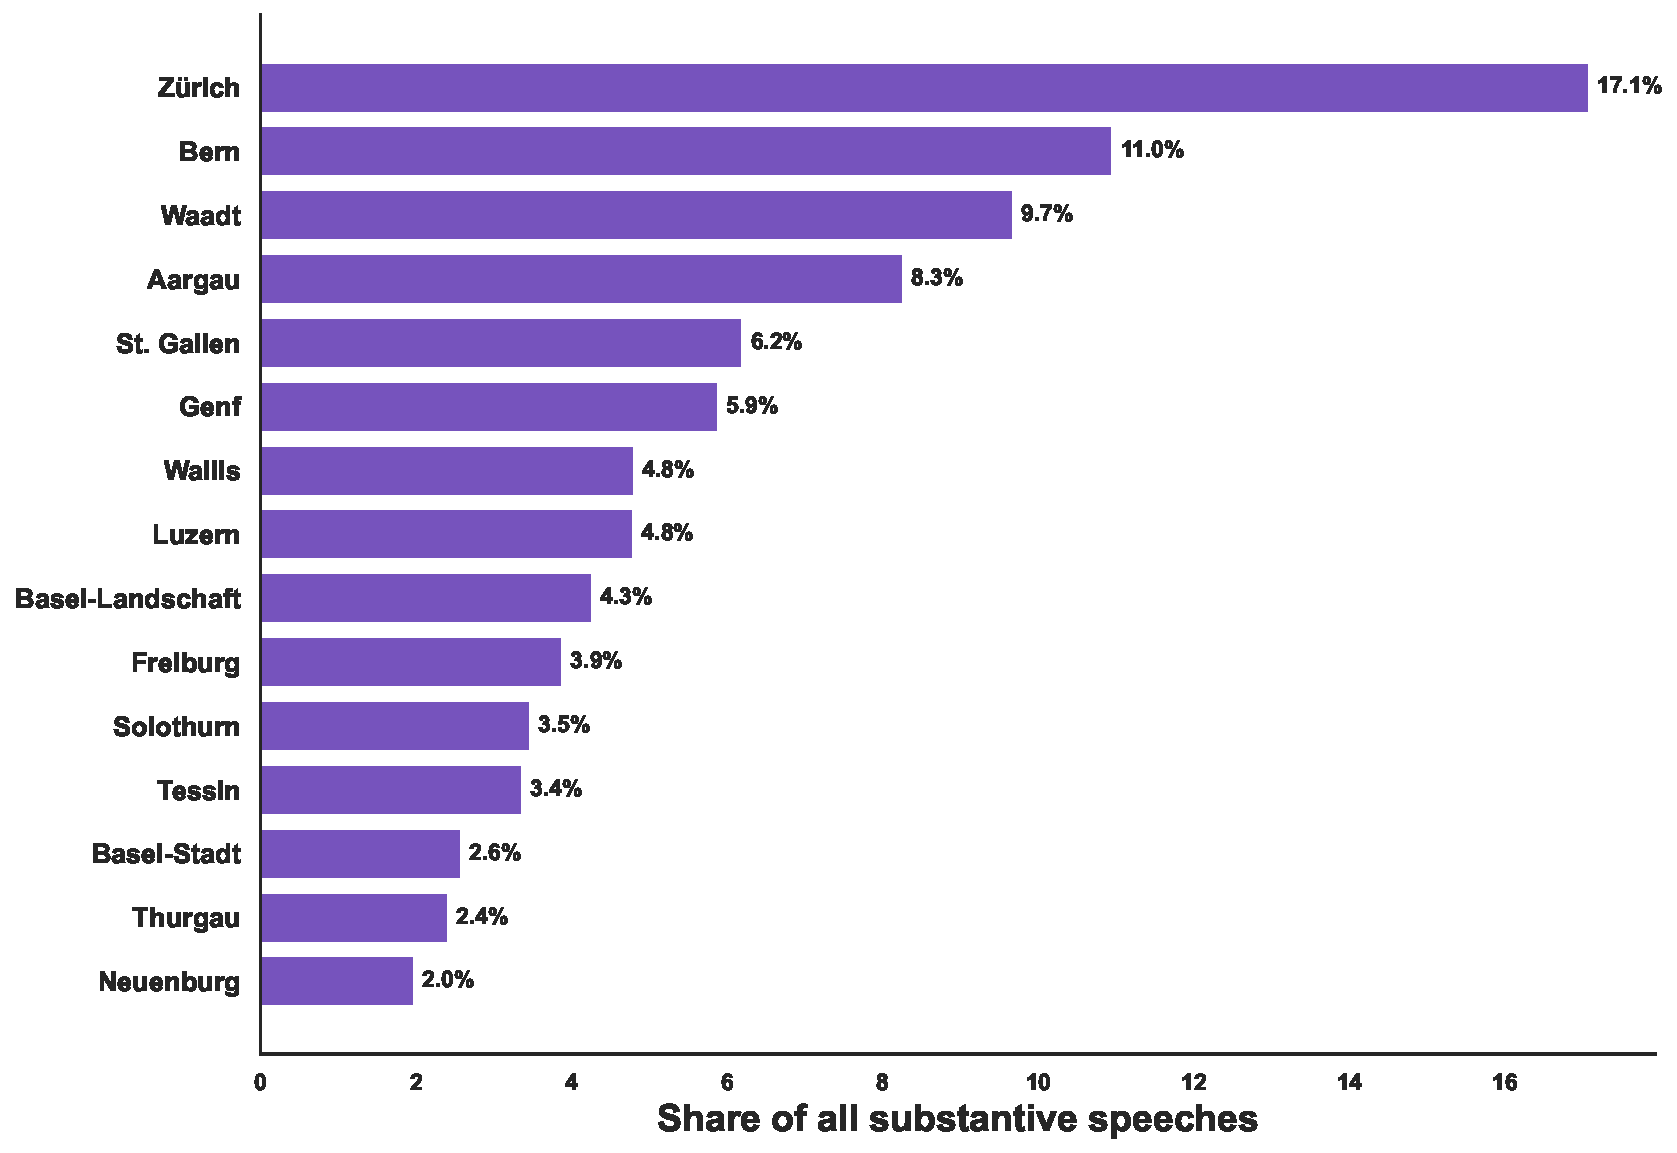
\includegraphics[width=0.70\textwidth,height=0.82\textheight,keepaspectratio]{fig_lt_canton_share.pdf}
    \end{frame}
\begin{frame}{Canton Speeches per MP --- Nationalrat}
    \centering
    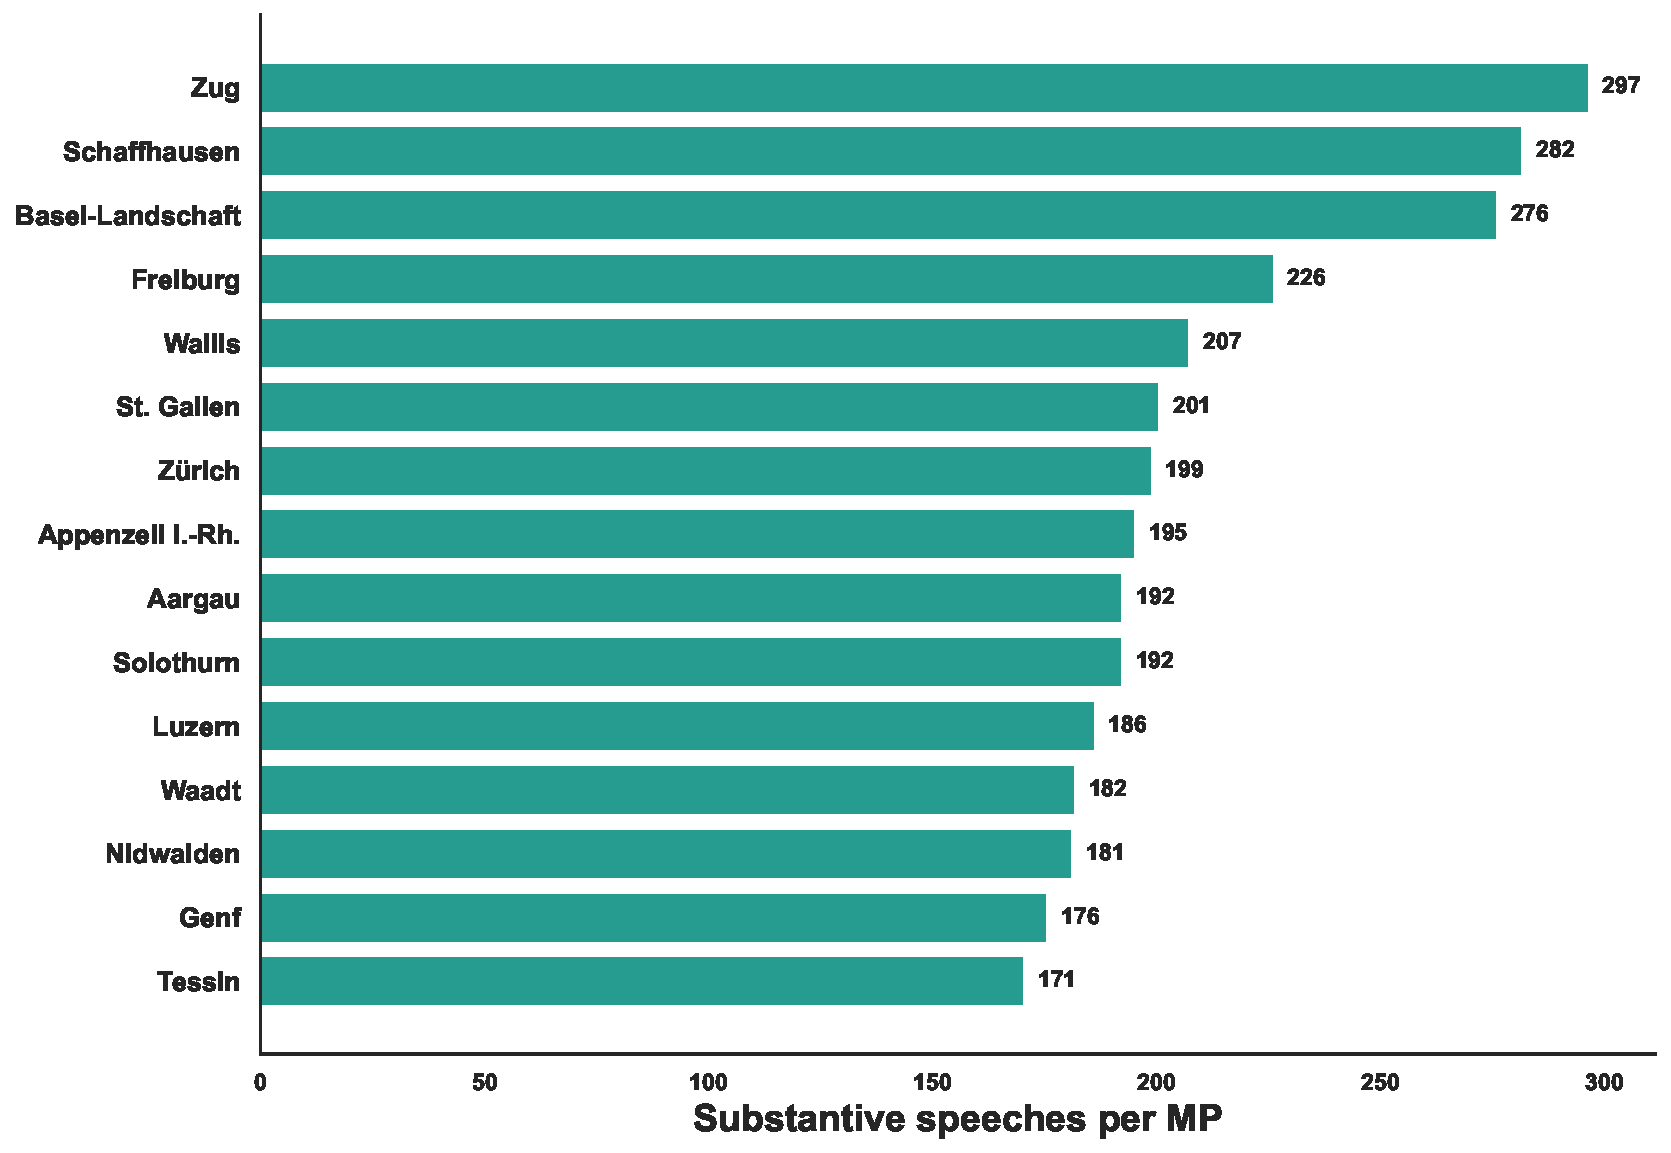
\includegraphics[width=0.78\textwidth,height=0.82\textheight,keepaspectratio]{fig_lt_canton_per_mp.pdf}
    \end{frame}
\begin{frame}{Floor-Time Gap by Canton --- Nationalrat}
    \centering
    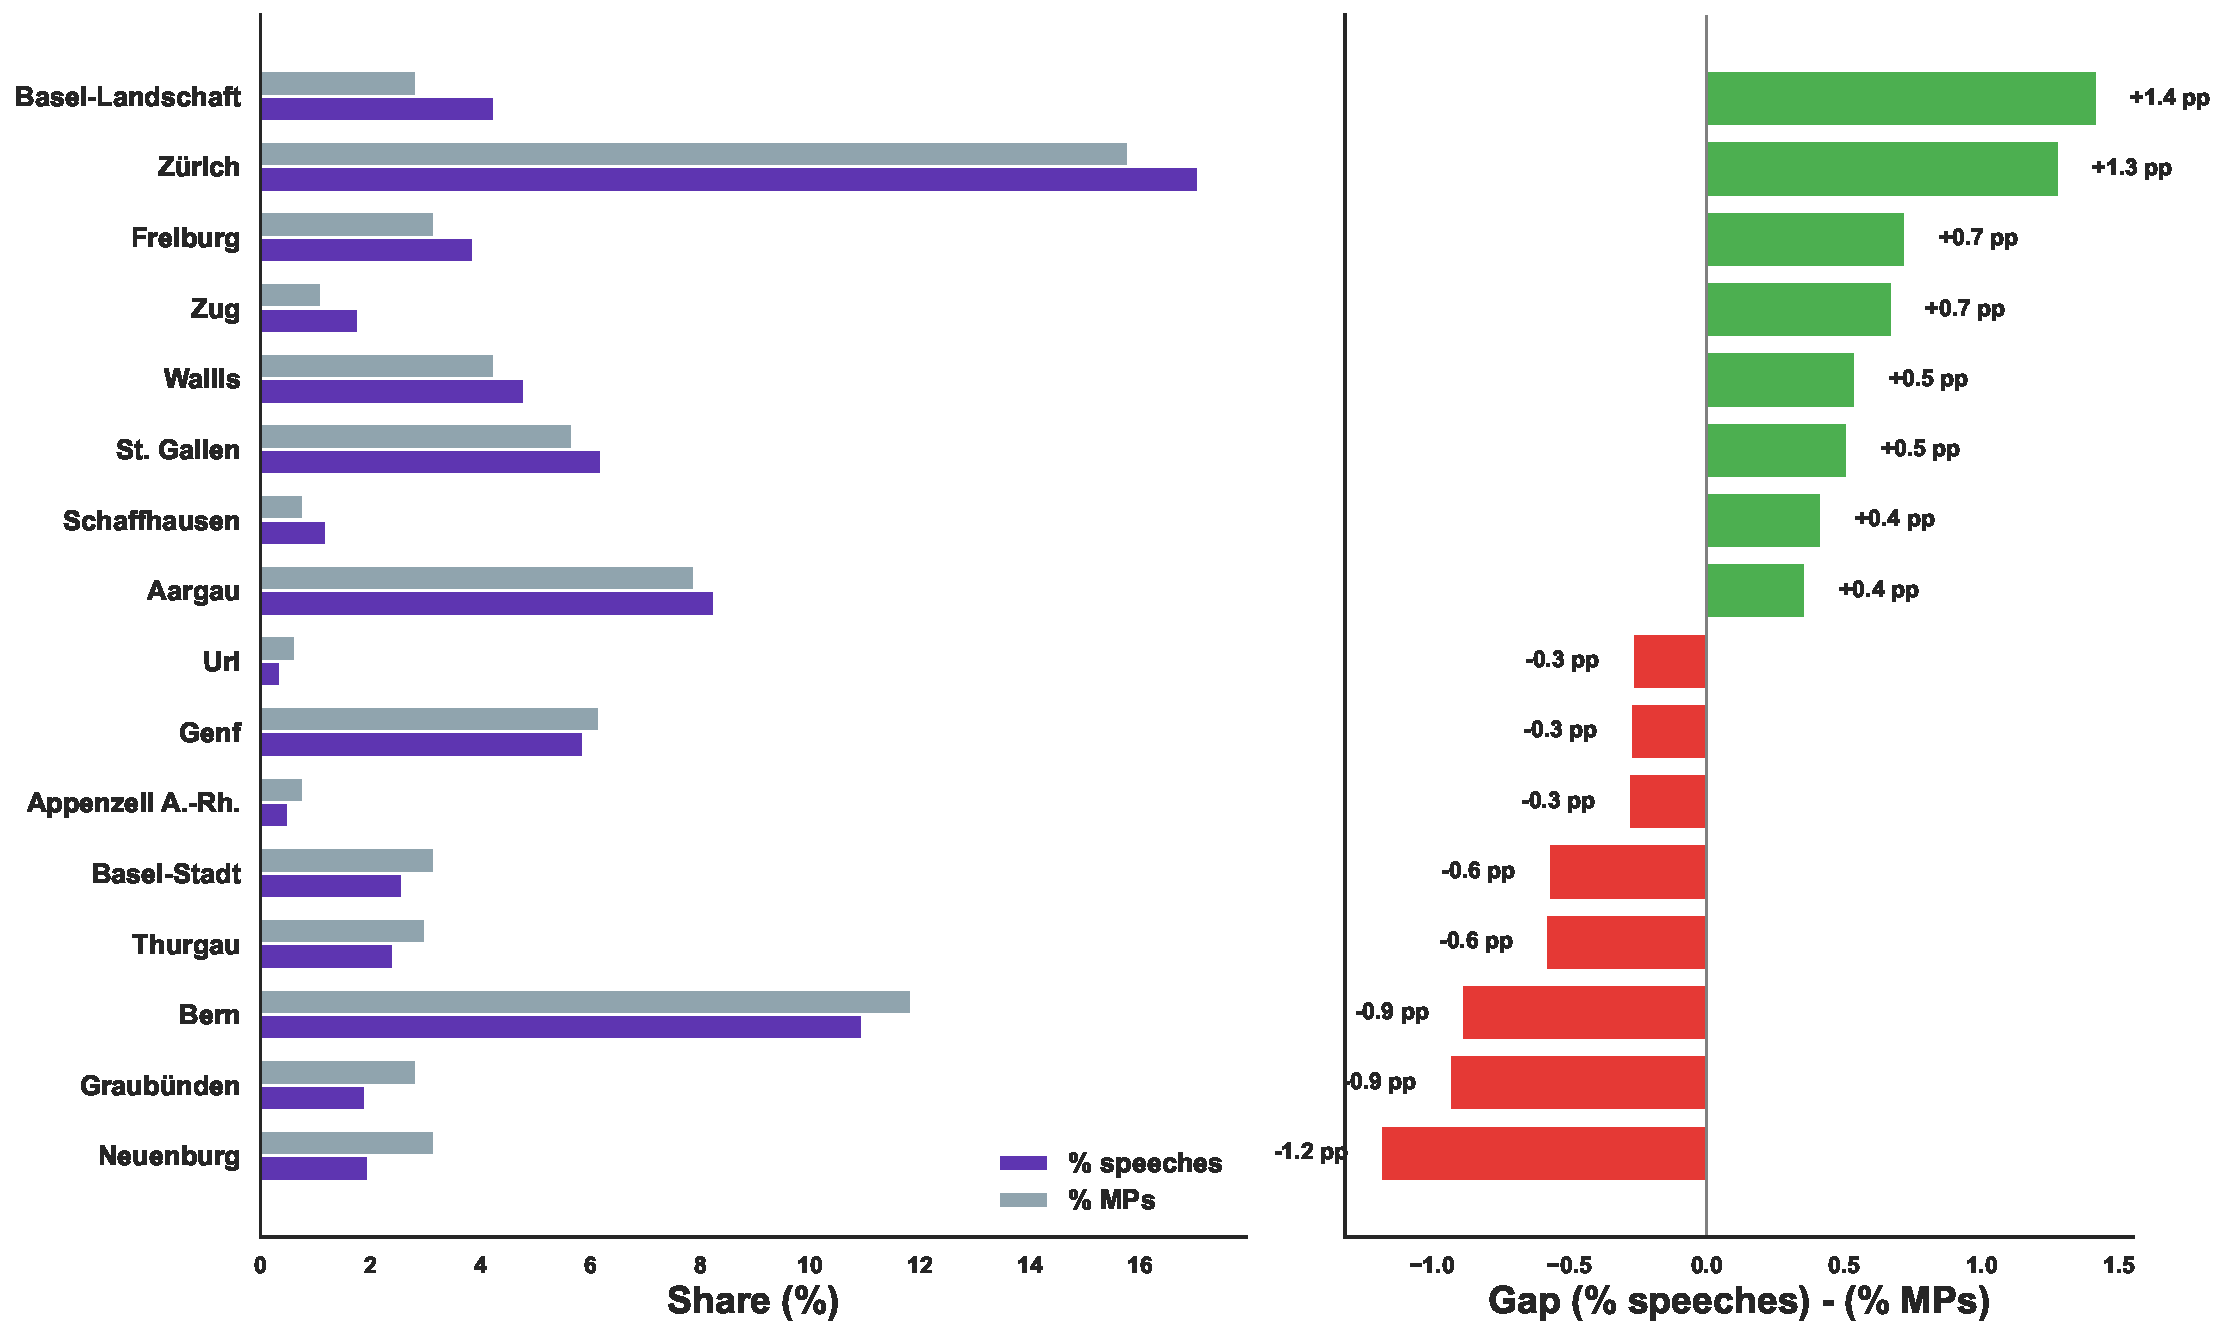
\includegraphics[width=0.88\textwidth,height=0.82\textheight,keepaspectratio]{fig_lt_canton_gap.pdf}
    \end{frame}
\begin{frame}{SVP Anger Before and After 2007 --- Nationalrat}
    \centering
    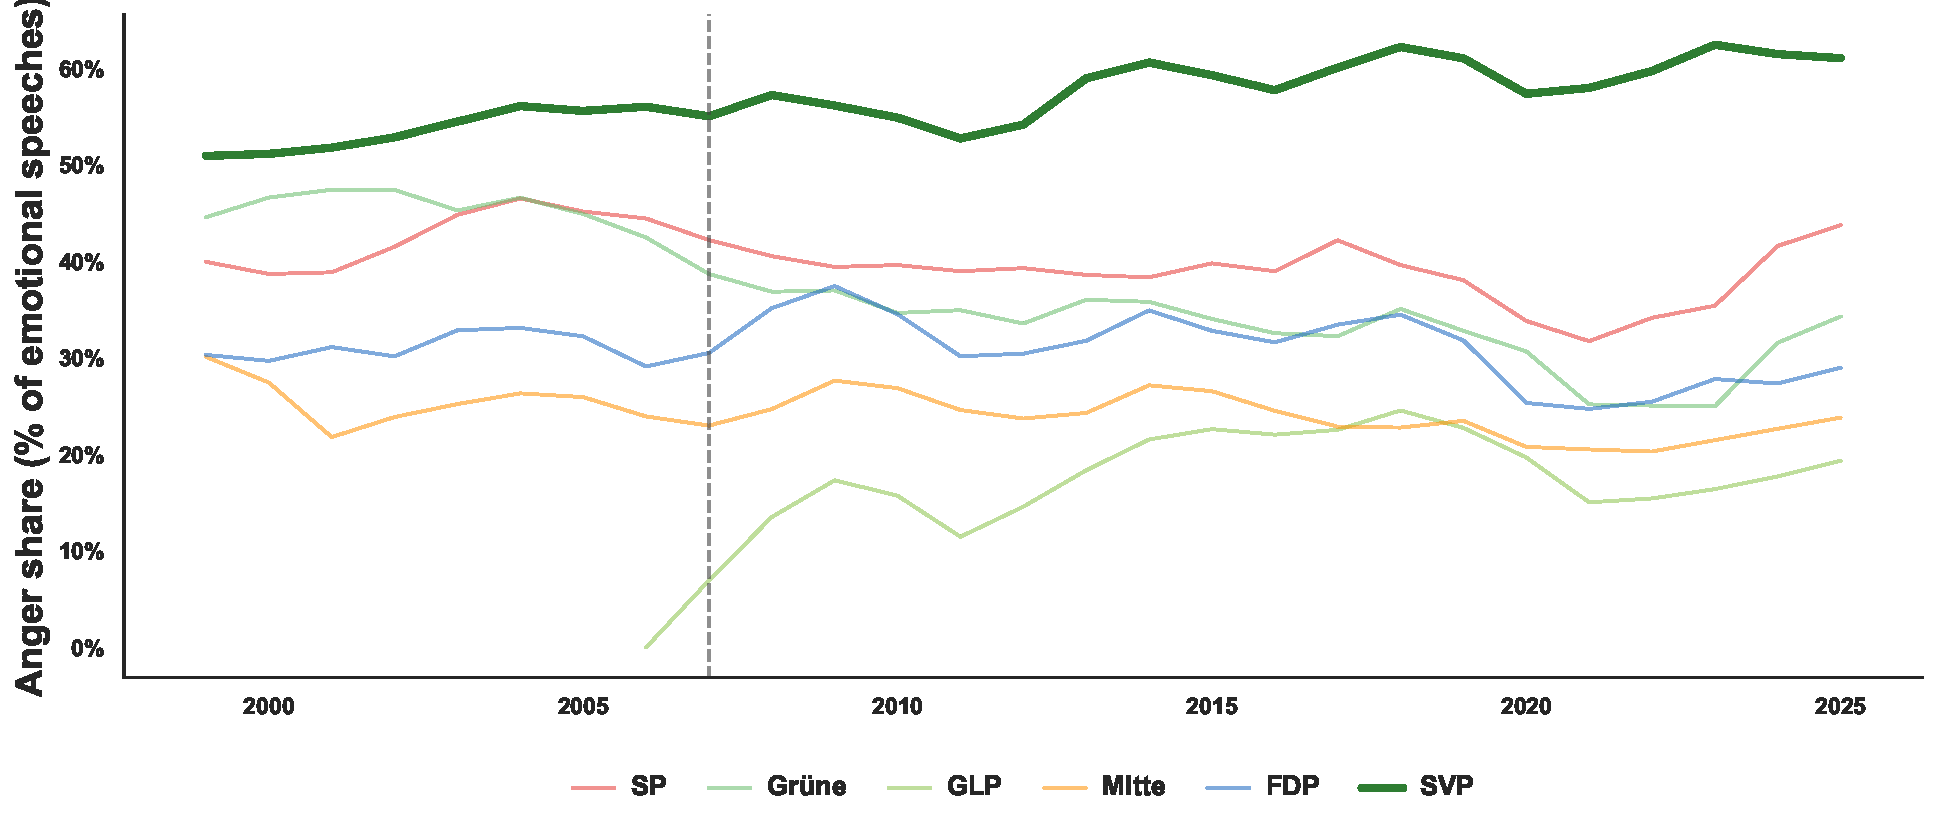
\includegraphics[width=0.82\textwidth,height=0.82\textheight,keepaspectratio]{fig_lt_udc_blocher_anger.pdf}
    \end{frame}
\begin{frame}{Anger Pre-2007 vs Post-2007 by Party --- Nationalrat}
\centering
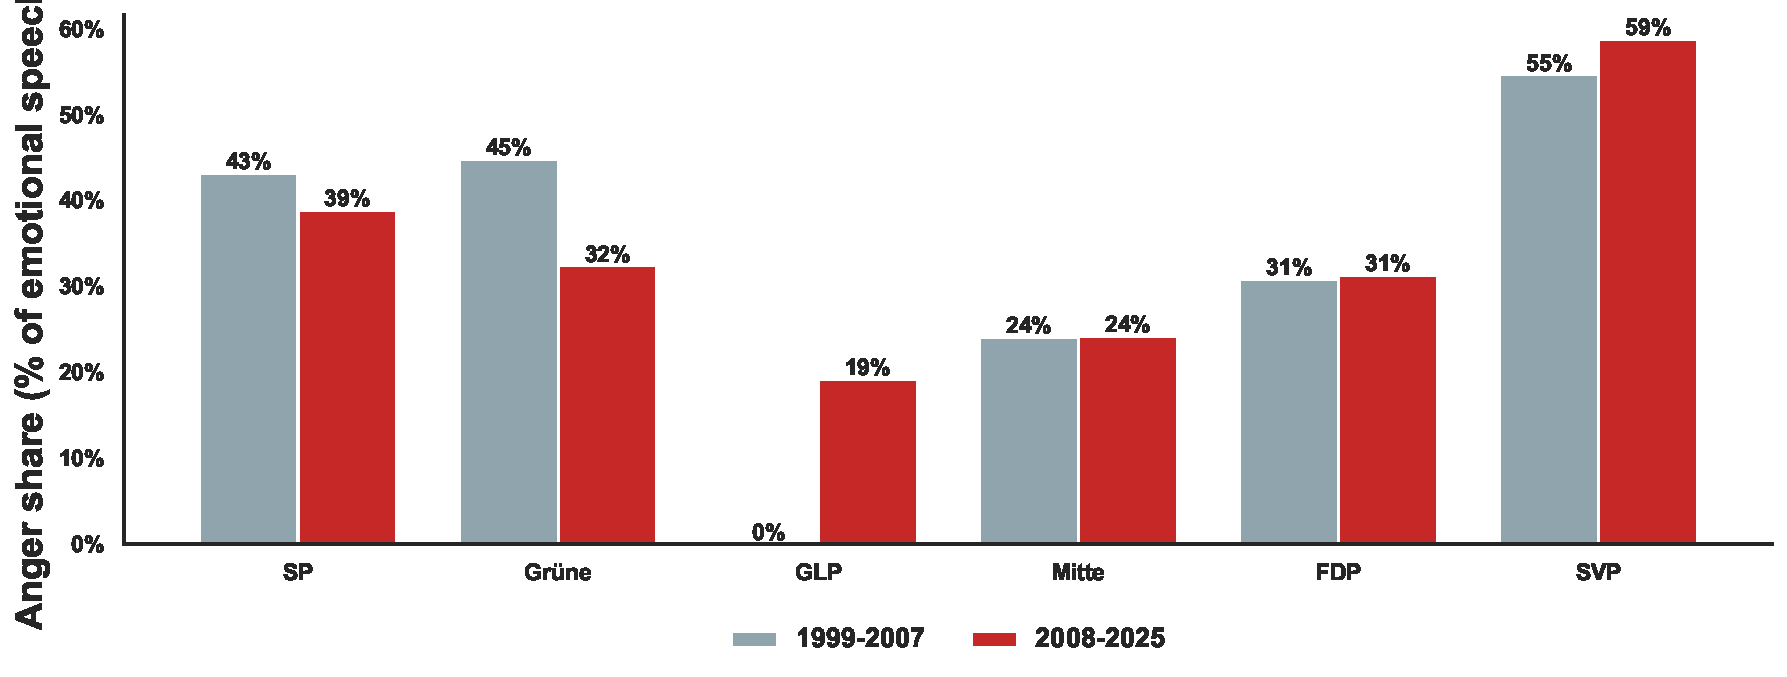
\includegraphics[width=0.85\textwidth,height=0.76\textheight,keepaspectratio]{fig_lt_udc_blocher_prepost.pdf}
\vfill
{\footnotesize\textit{Note:} GLP (PVL) enters the National Council only after the October 2007 election; its pre-2008 bar is based on a tiny winter-session slice and should be treated as illustrative only.}
\end{frame}
\begin{frame}{Emotional Rhetoric by Generation of MPs --- Nationalrat}
\centering
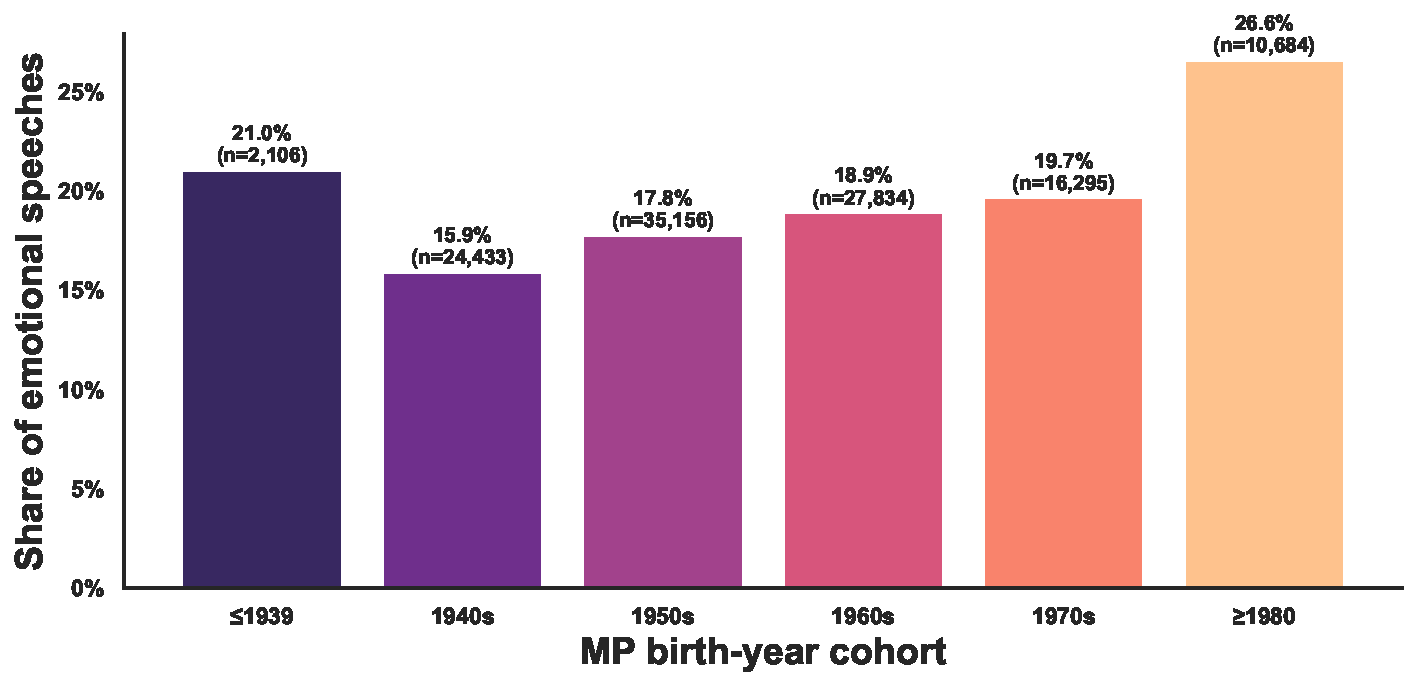
\includegraphics[width=0.82\textwidth,height=0.76\textheight,keepaspectratio]{fig_lt_cohort_emotional.pdf}
\vfill
{\footnotesize\textit{Note:} Younger birth cohorts appear here mostly at ages under~50; older cohorts mostly over~50 in this corpus window. Level differences can mix a \textbf{cohort} story with an \textbf{age-at-speech} story; the next slide (age groups) is complementary but does not fully separate the two.}
\end{frame}
\begin{frame}{Emotional Rhetoric by Age Group --- Nationalrat}
    \centering
    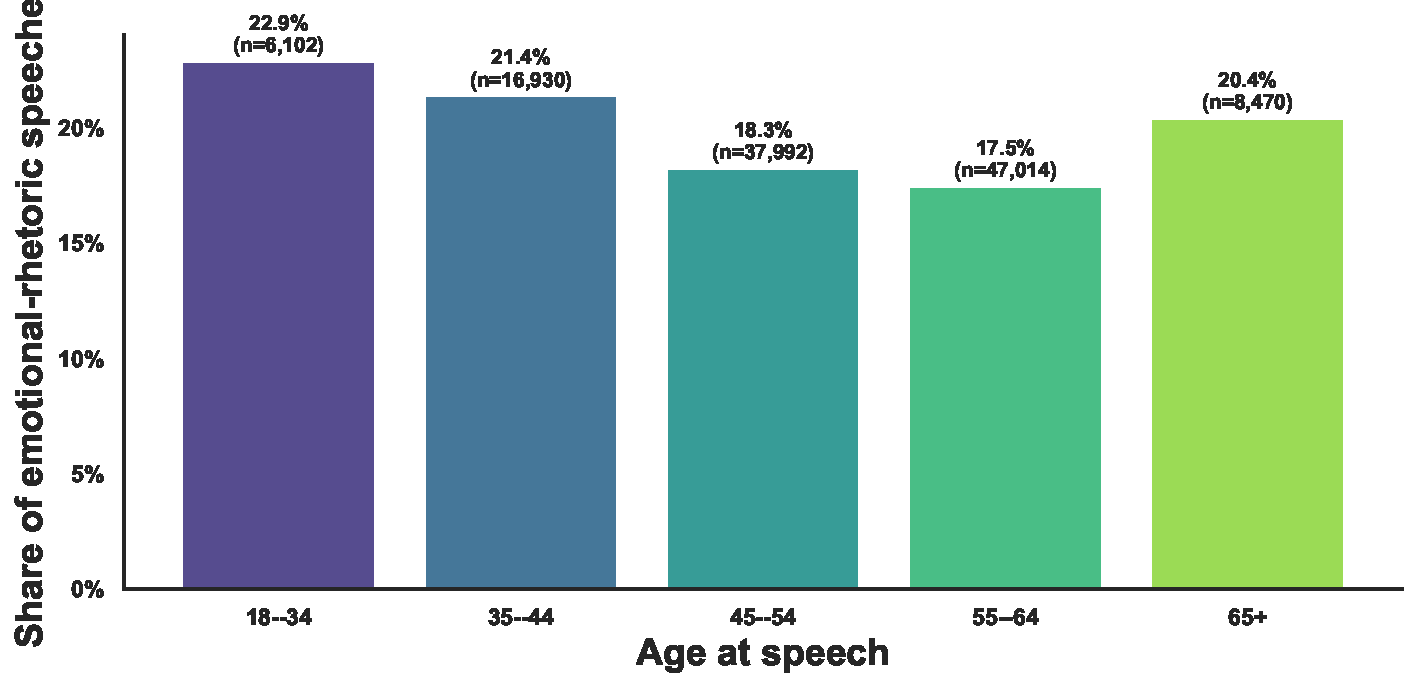
\includegraphics[width=0.82\textwidth,height=0.82\textheight,keepaspectratio]{fig_lt_age_group_emotional.pdf}
    \end{frame}
\begin{frame}{Emotional Rhetoric by Language of the Speech --- Nationalrat}
    \centering
    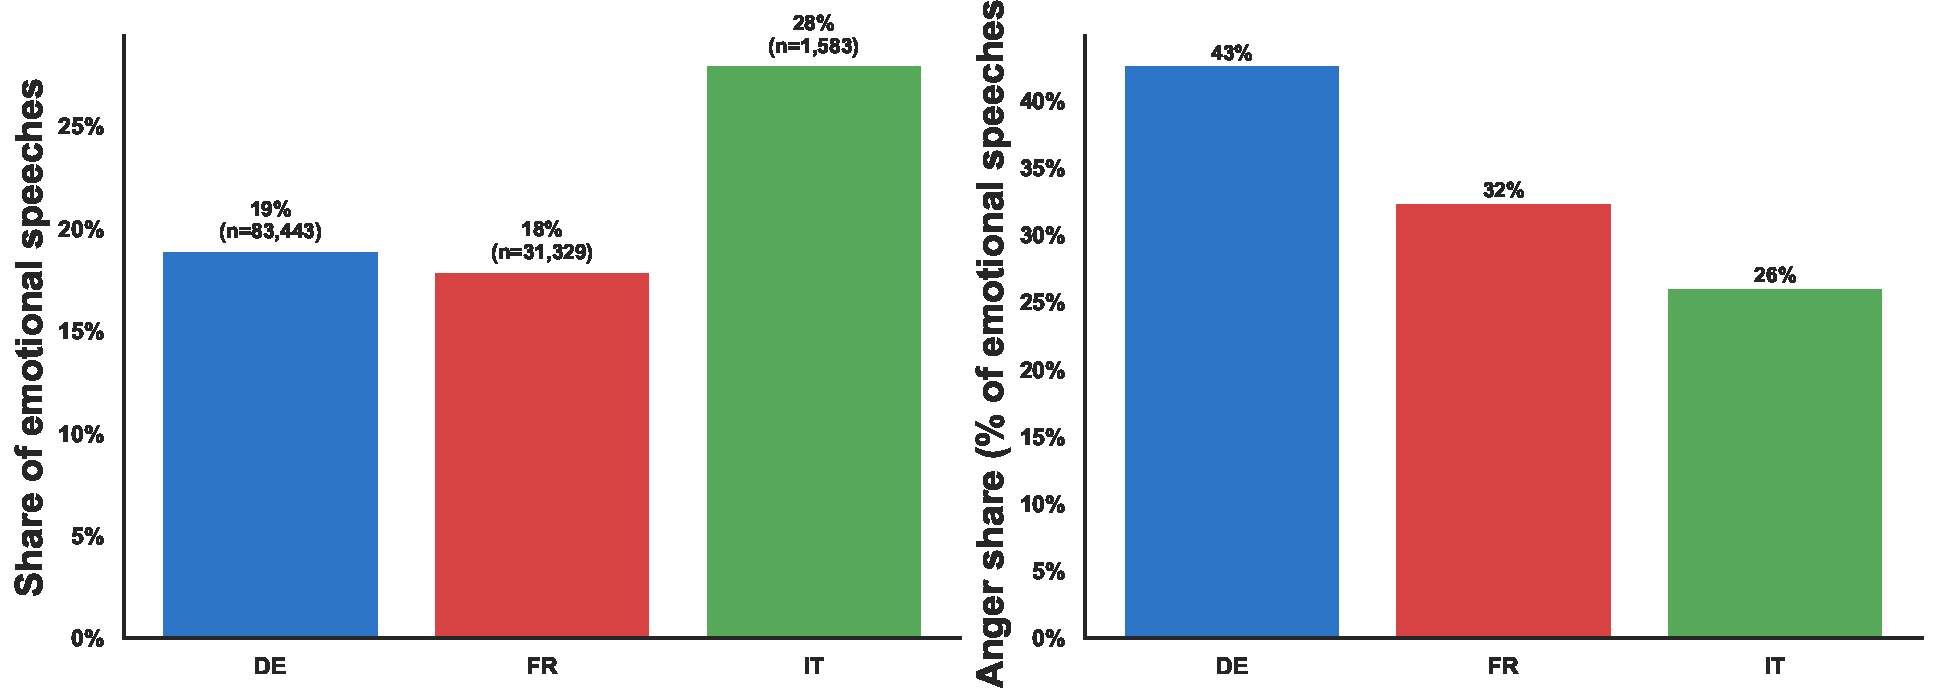
\includegraphics[width=0.95\textwidth,height=0.82\textheight,keepaspectratio]{fig_lt_emotion_language.pdf}
    \end{frame}
\begin{frame}{Applause by Party --- Nationalrat}
\begin{columns}[T]
\begin{column}{0.49\textwidth}
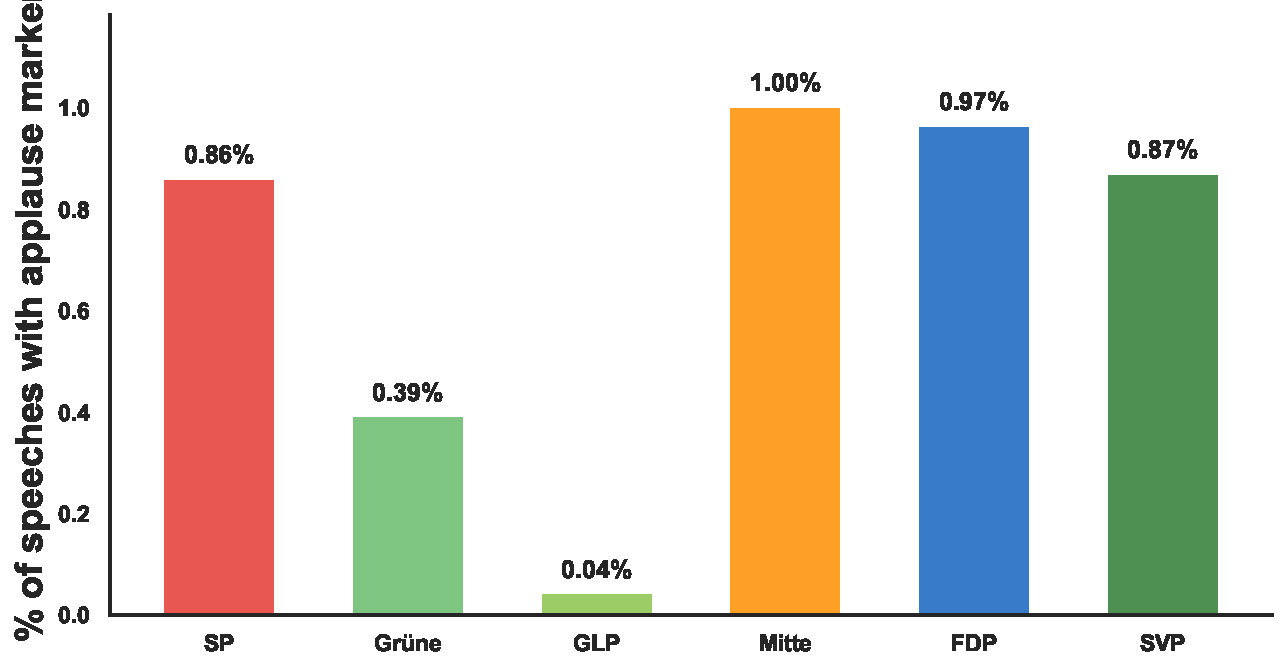
\includegraphics[width=\textwidth]{fig_app_rate_by_party.pdf}
\end{column}
\begin{column}{0.49\textwidth}
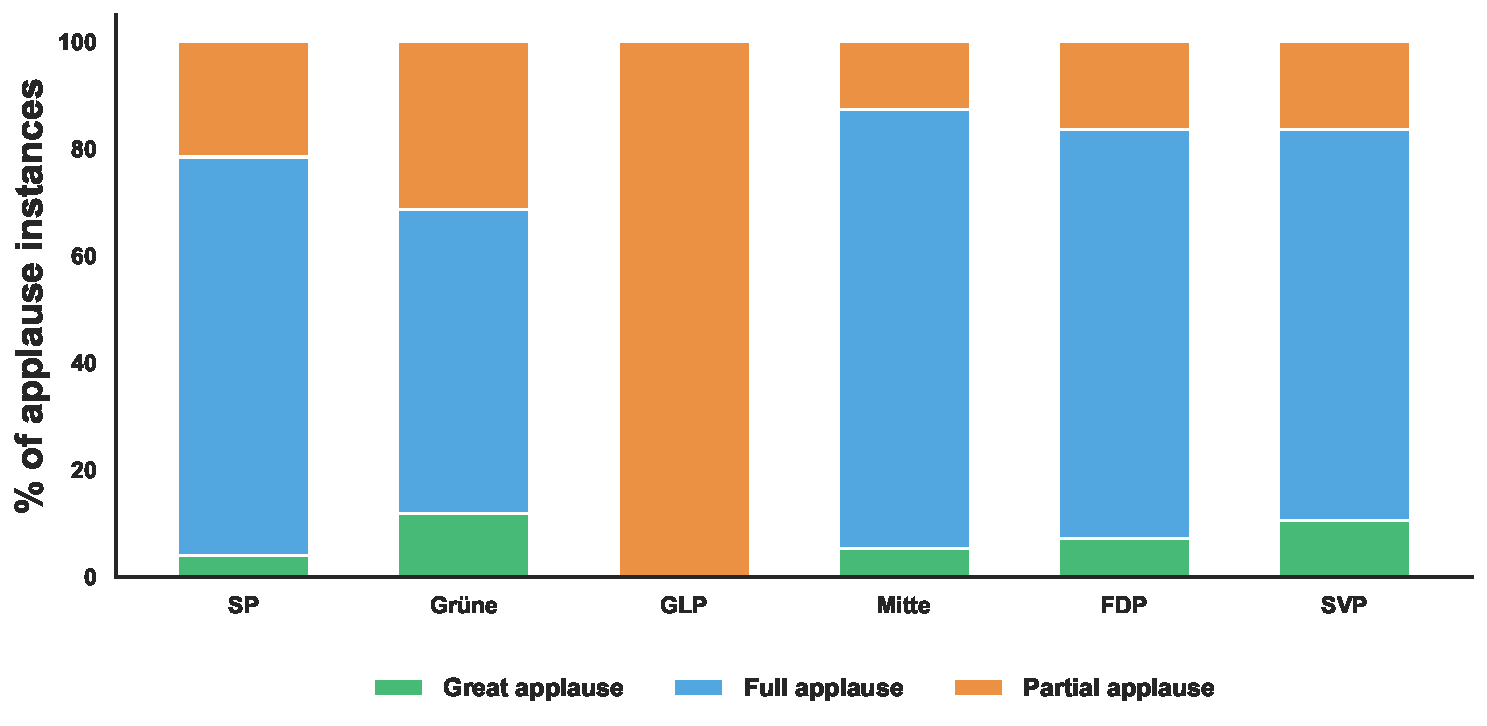
\includegraphics[width=\textwidth]{fig_app_type_by_party.pdf}
\end{column}
\end{columns}
\end{frame}
\begin{frame}{Most Applauded Parliamentarians --- Nationalrat}
    \centering
    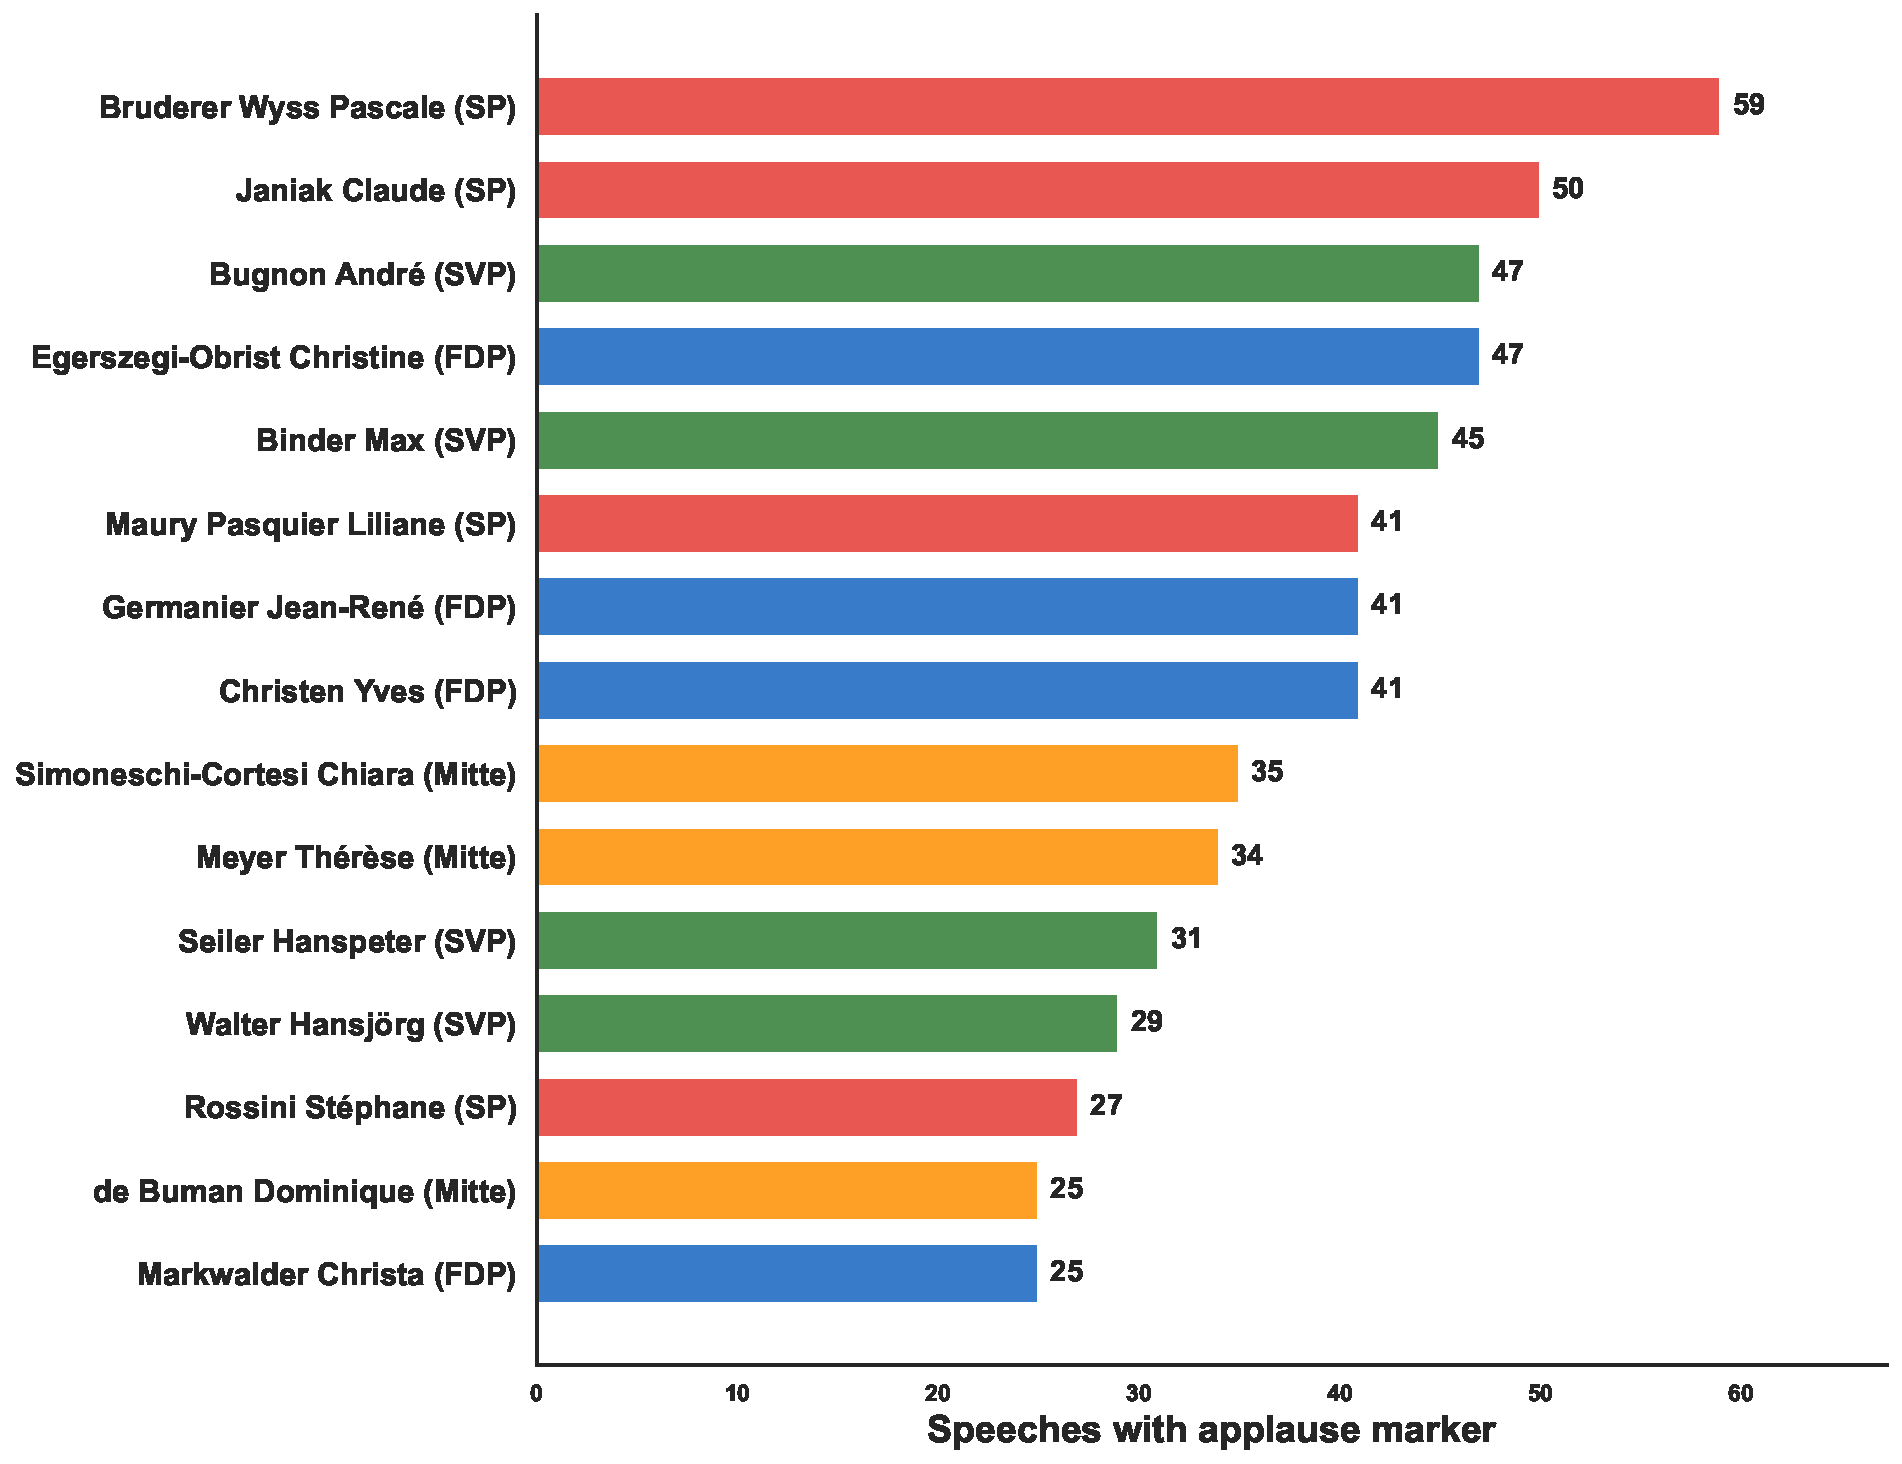
\includegraphics[width=0.96\textwidth,height=0.82\textheight,keepaspectratio]{fig_app_top_mps.pdf}
    \end{frame}

%========================================================================================
% PART II — STÄNDERAT
%========================================================================================

\section{Part II: Ständerat}
\begin{frame}{}
\vfill
\centering
\hypertarget{part.SR}{}
{\Large \textbf{Part II: Ständerat}}
\vfill
\end{frame}

\begin{frame}{Floor Time Share by Party --- Ständerat}
\hypertarget{main.SR.floor}{}
\centering
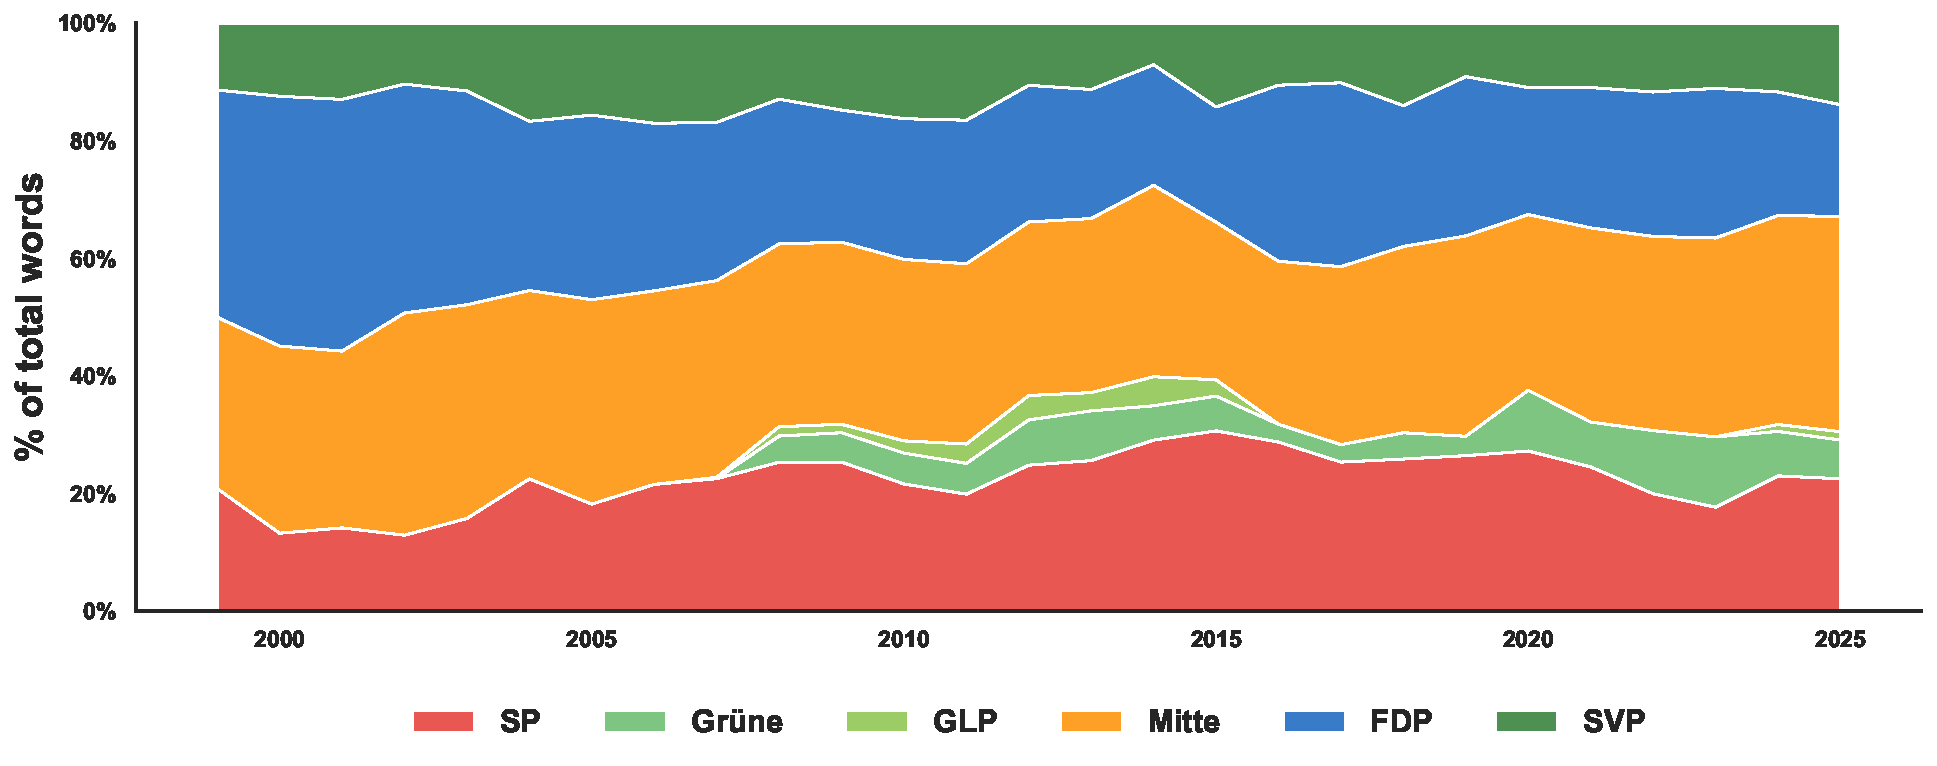
\includegraphics[width=0.92\textwidth,height=0.76\textheight,keepaspectratio]{staenderat_desc_06_floor_time_share.pdf}
\vfill
{\footnotesize Detailed Ständerat topic checks are in the \hyperlink{app.SR.topic}{appendix}.}
\end{frame}
\begin{frame}{Topic Shift --- Ständerat}
\hypertarget{main.SR.topic}{}
\centering
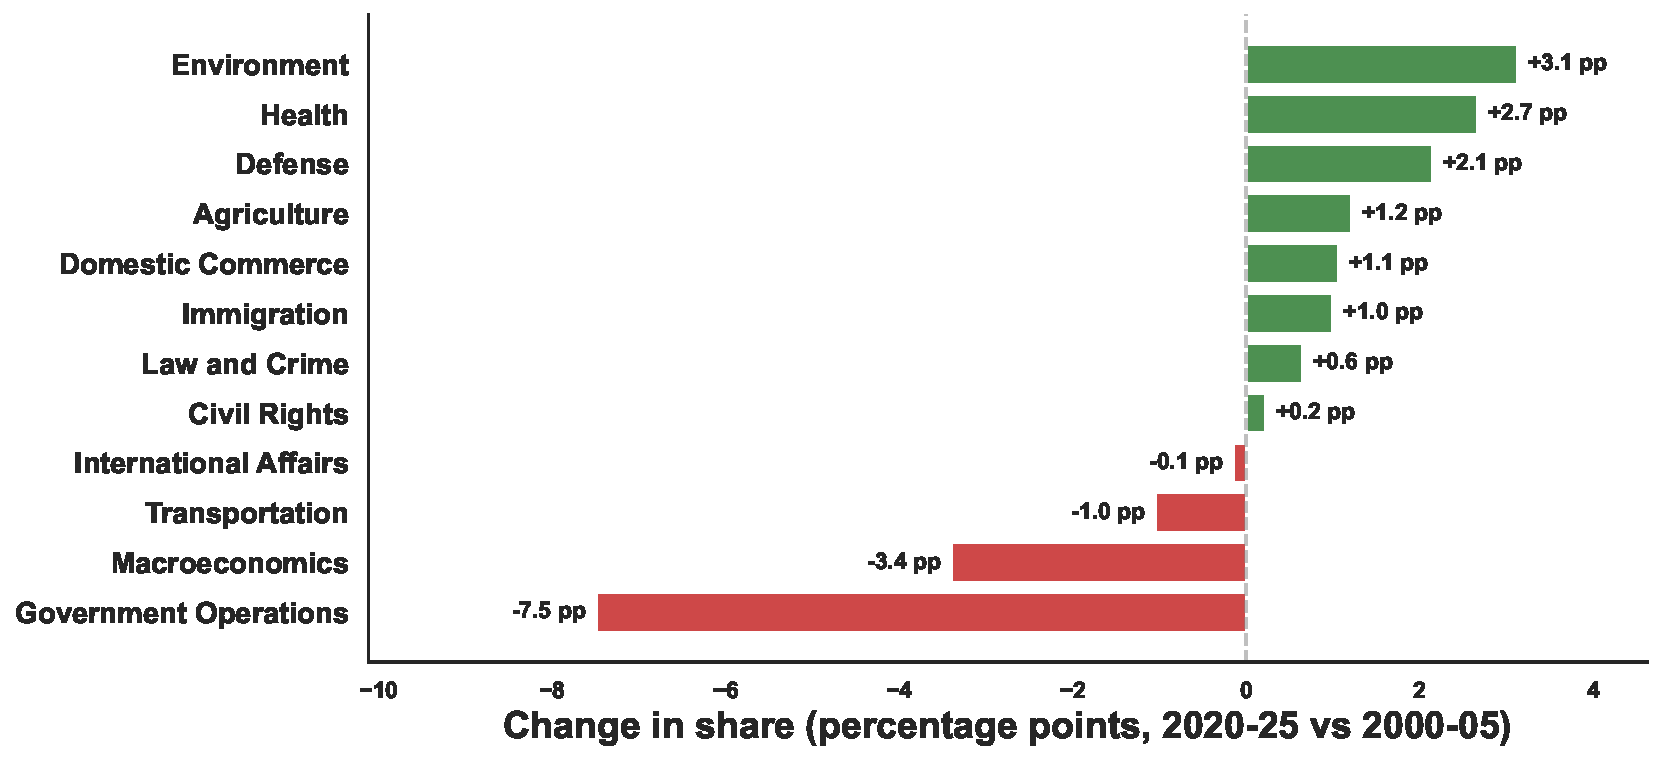
\includegraphics[width=0.82\textwidth,height=0.76\textheight,keepaspectratio]{staenderat_fig_lt_topic_shift_noproc.pdf}
\vfill
{\footnotesize \hyperlink{app.SR.topic}{Appendix: topic distribution, relative shift, party drivers}.}
\end{frame}
\begin{frame}{Emotional Rhetoric --- Ständerat}
\hypertarget{main.SR.emotion}{}
\centering
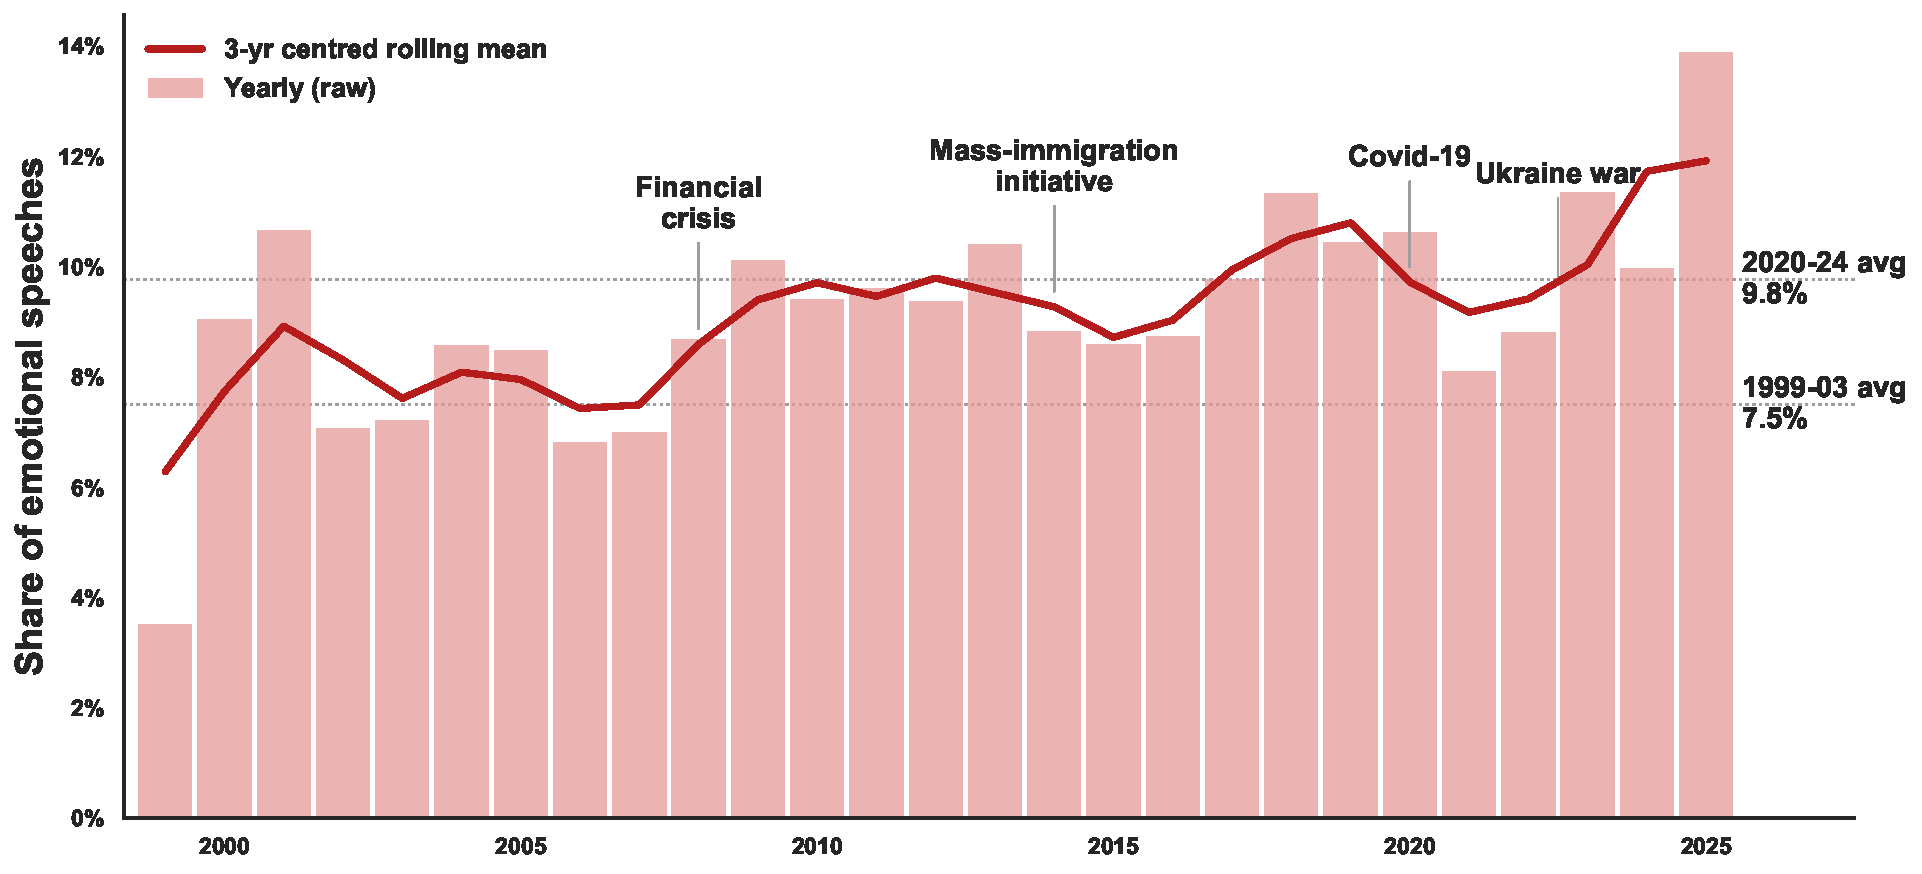
\includegraphics[width=0.92\textwidth,height=0.76\textheight,keepaspectratio]{staenderat_fig_lt_defD_overall_time.pdf}
\vfill
{\footnotesize \hyperlink{app.SR.emotion}{Appendix: party, legislature and topic emotion checks}.}
\end{frame}
\begin{frame}{Dominant Emotion in Emotional Speeches --- Ständerat}
\centering
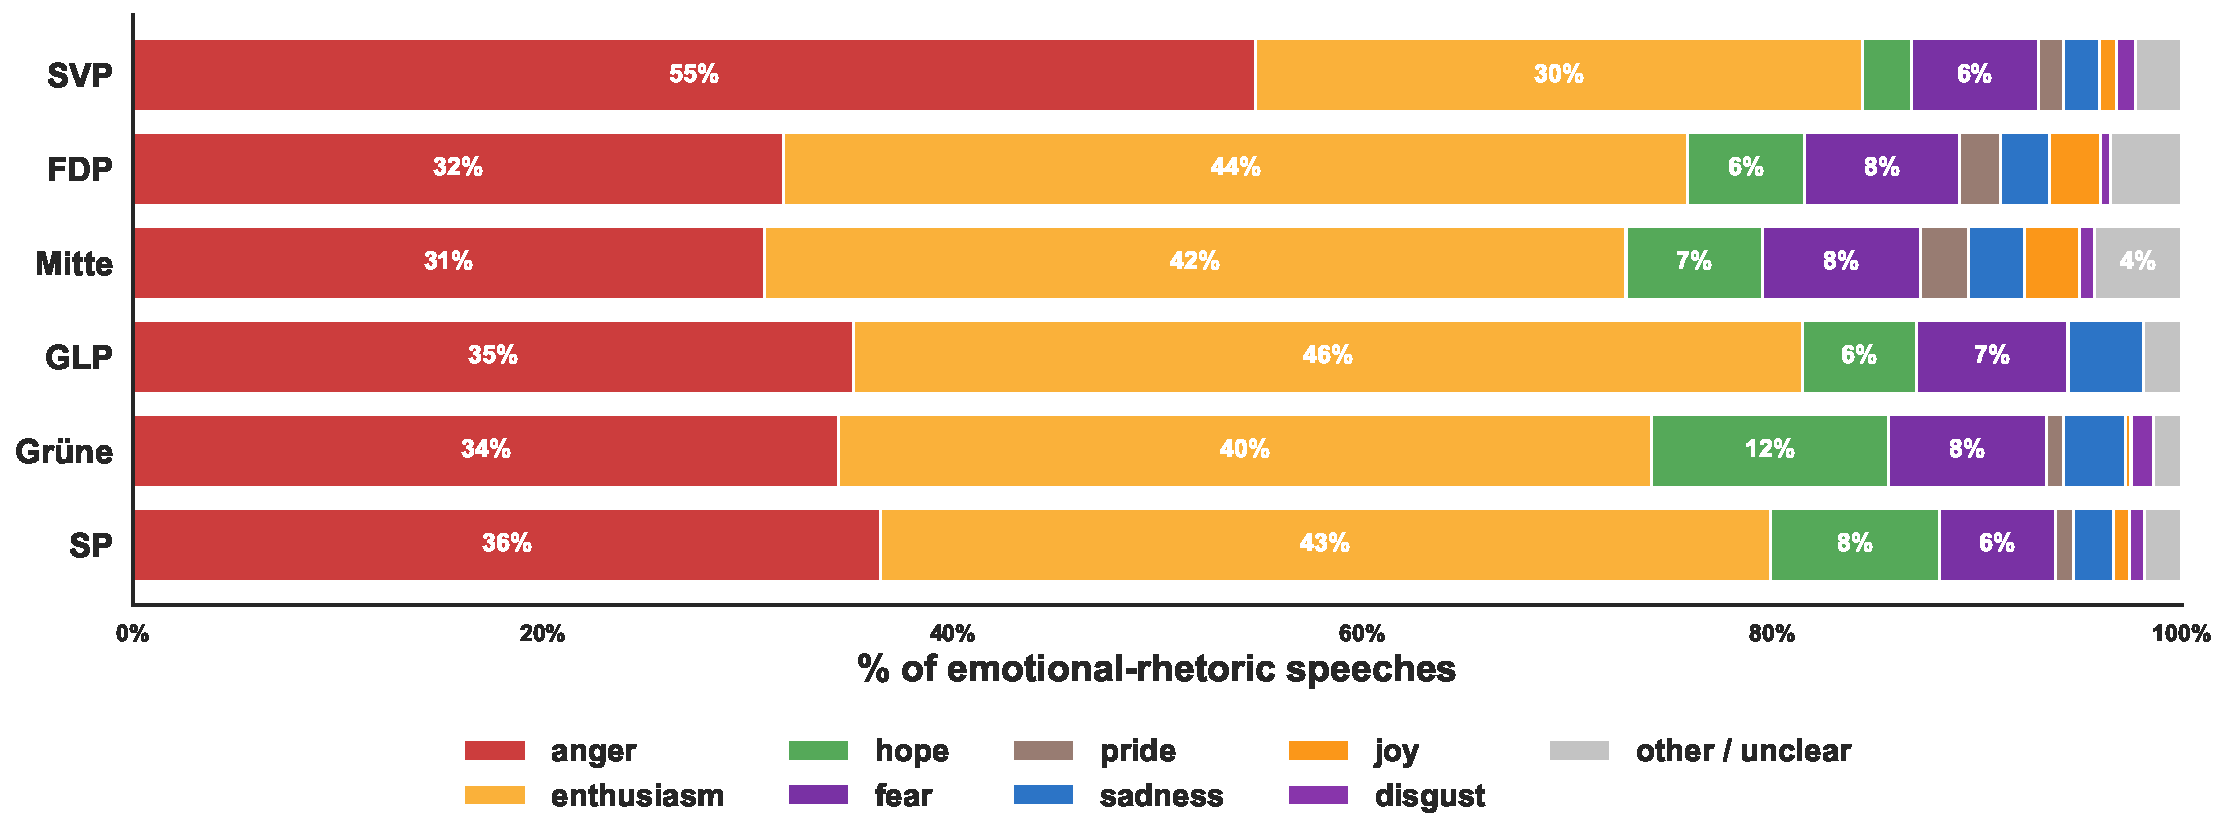
\includegraphics[width=0.92\textwidth,height=0.76\textheight,keepaspectratio]{staenderat_fig_lt_llm_dominant_party.pdf}
\vfill
{\footnotesize \hyperlink{app.SR.emotion}{Appendix: Ständerat emotion robustness figures}.}
\end{frame}
\begin{frame}{Floor-Time Gap by Gender --- Ständerat (1999--2025)}
\hypertarget{main.SR.gender}{}
\centering
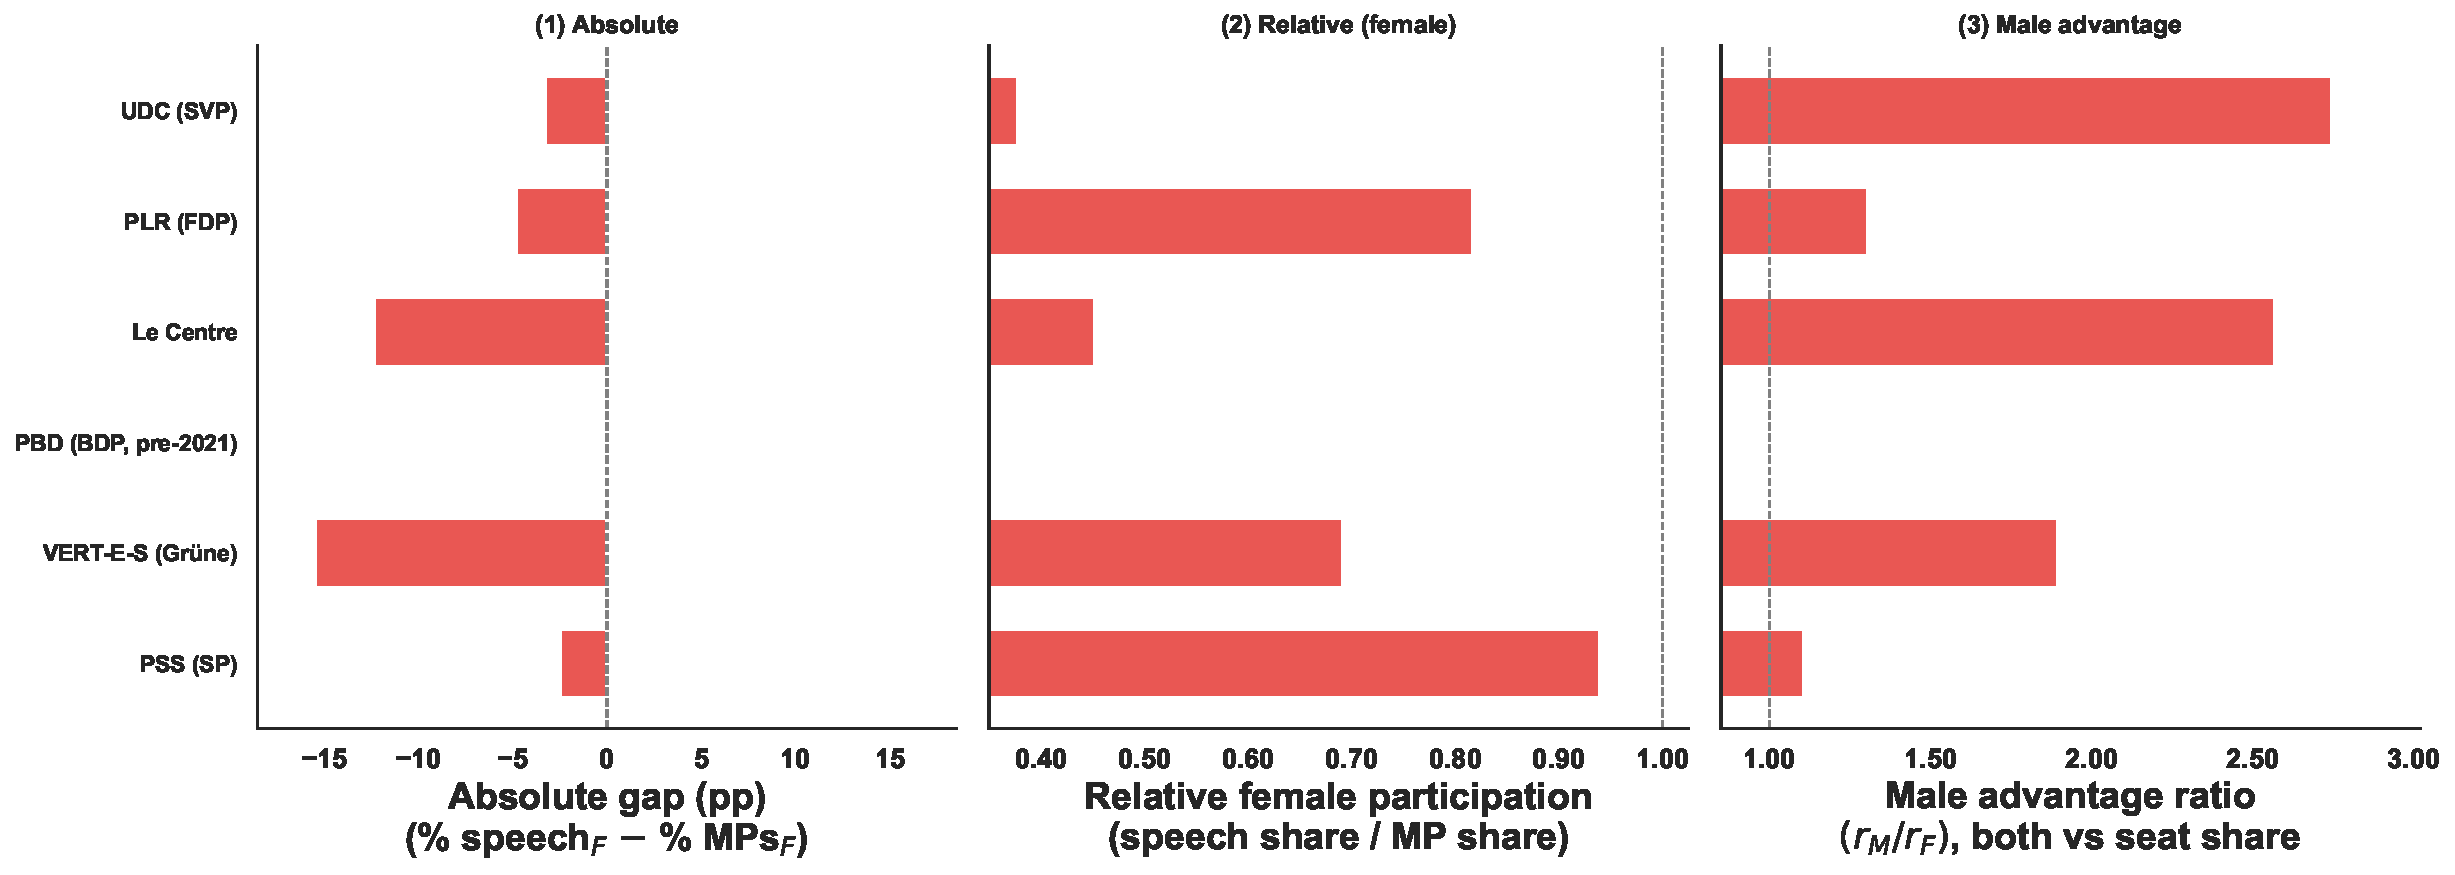
\includegraphics[width=0.95\textwidth,height=0.76\textheight,keepaspectratio]{fig_lt_gender_metrics_bars_1999_2025_staenderat.pdf}
\vfill
{\footnotesize \hyperlink{app.SR.gender}{Appendix: Ständerat gender, canton, age, language and applause checks}.}
\end{frame}

\begin{frame}{Appendix Preview --- Detailed Ständerat Checks}
\centering
\small
\begin{itemize}\setlength\itemsep{0.7em}
\item \hyperlink{app.SR.topic}{Topic distribution, relative shift and party drivers}
\item \hyperlink{app.SR.emotion}{Party, legislature and topic-level emotion checks}
\item \hyperlink{app.SR.gender}{Gender, canton, age, language and applause checks}
\end{itemize}
\end{frame}

%========================================================================================
% PART III — FOCUS (chamber comparison, benchmark, illustrations)
%========================================================================================

\section{Part III: Focus}
\begin{frame}{}
\vfill
\centering
\hypertarget{part.FOCUS}{}{\Large \textbf{Part III: Focus}}
\vfill
\end{frame}

\begin{frame}{Six Legislatures, One Method --- Existing Comparison}
\hypertarget{part.FOCUS.intl}{}
\centering
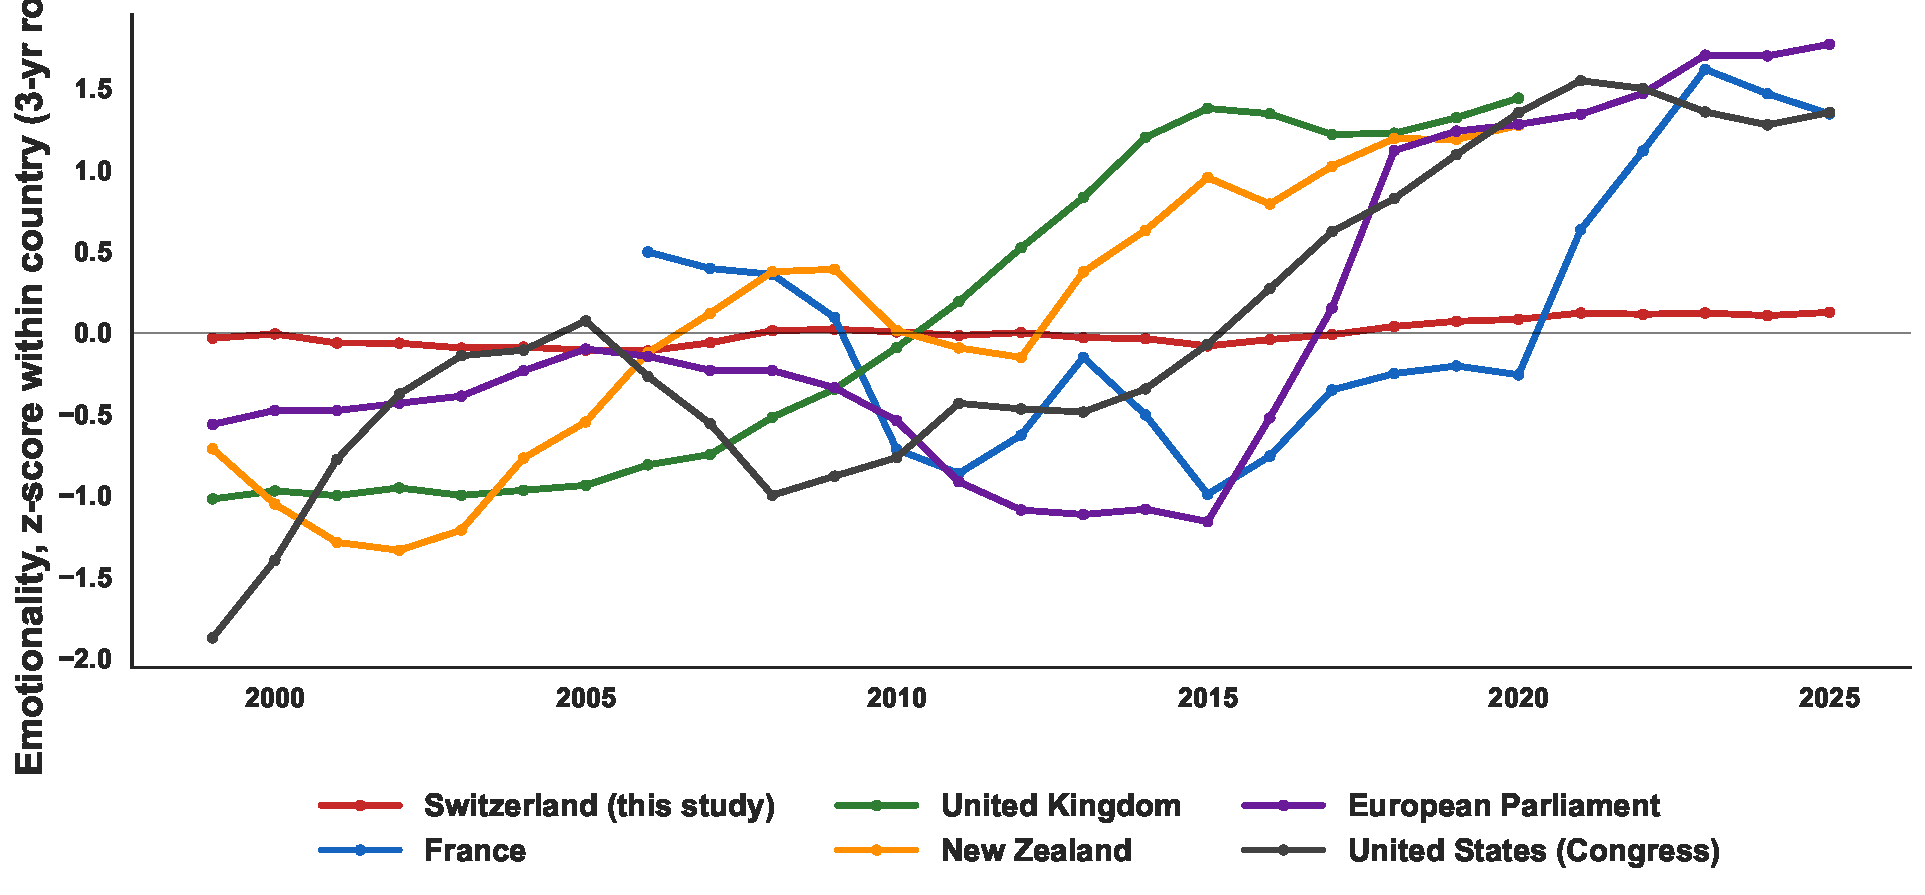
\includegraphics[width=0.88\textwidth,height=0.82\textheight,keepaspectratio]{fig_lt_country_emotionality_compare.pdf}
\end{frame}
\begin{frame}{National Council vs Council of States --- Emotional Share}
\hypertarget{part.FOCUS.chamber}{}
\centering
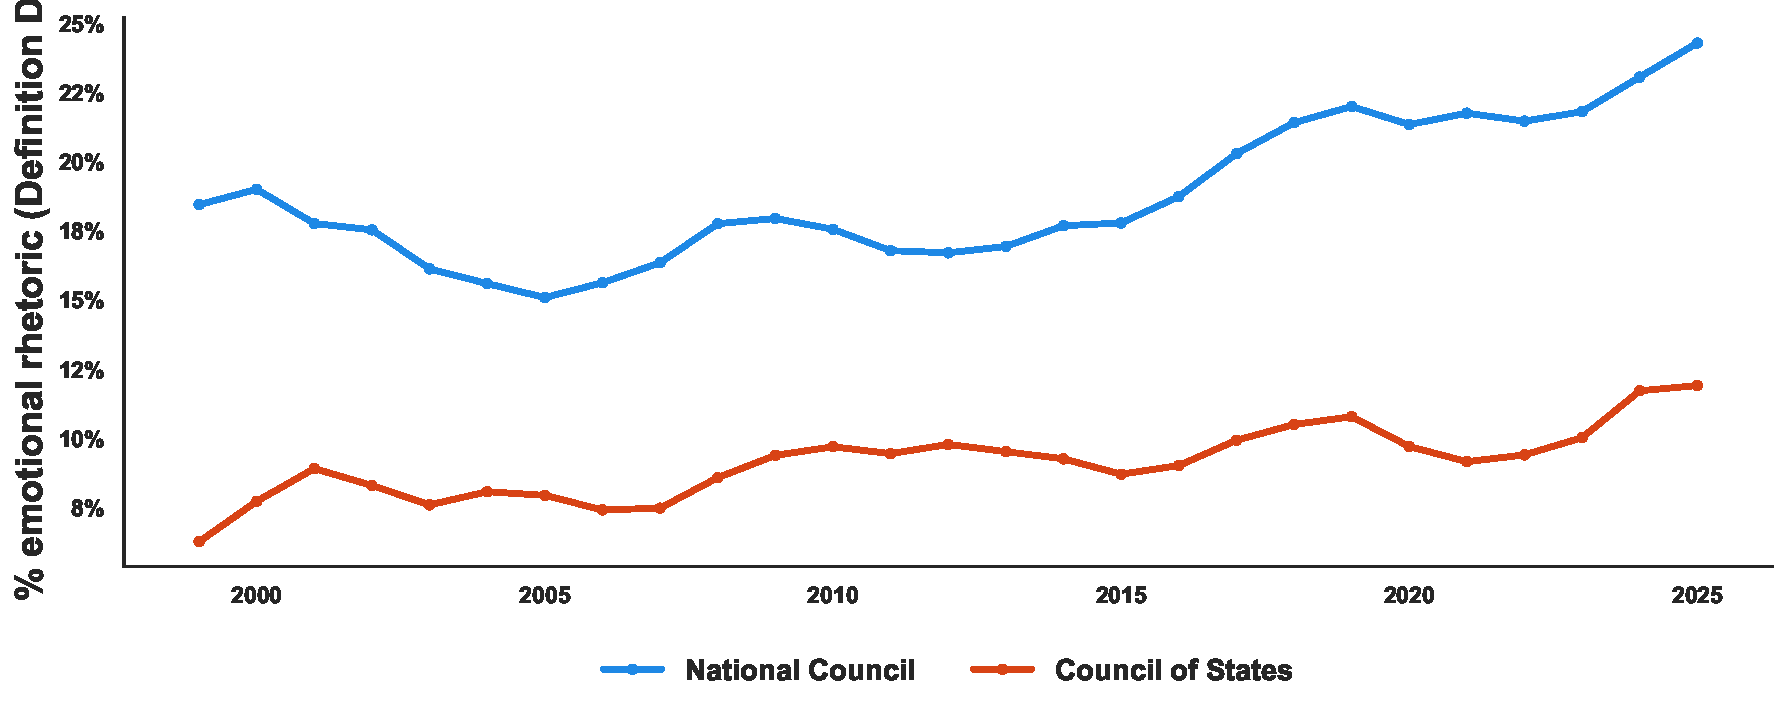
\includegraphics[width=0.82\textwidth,height=0.82\textheight,keepaspectratio]{fig_lt_council_emotional_defD_chambers.pdf}
\end{frame}
\begin{frame}{Anger Dominance by Chamber}
    \centering
    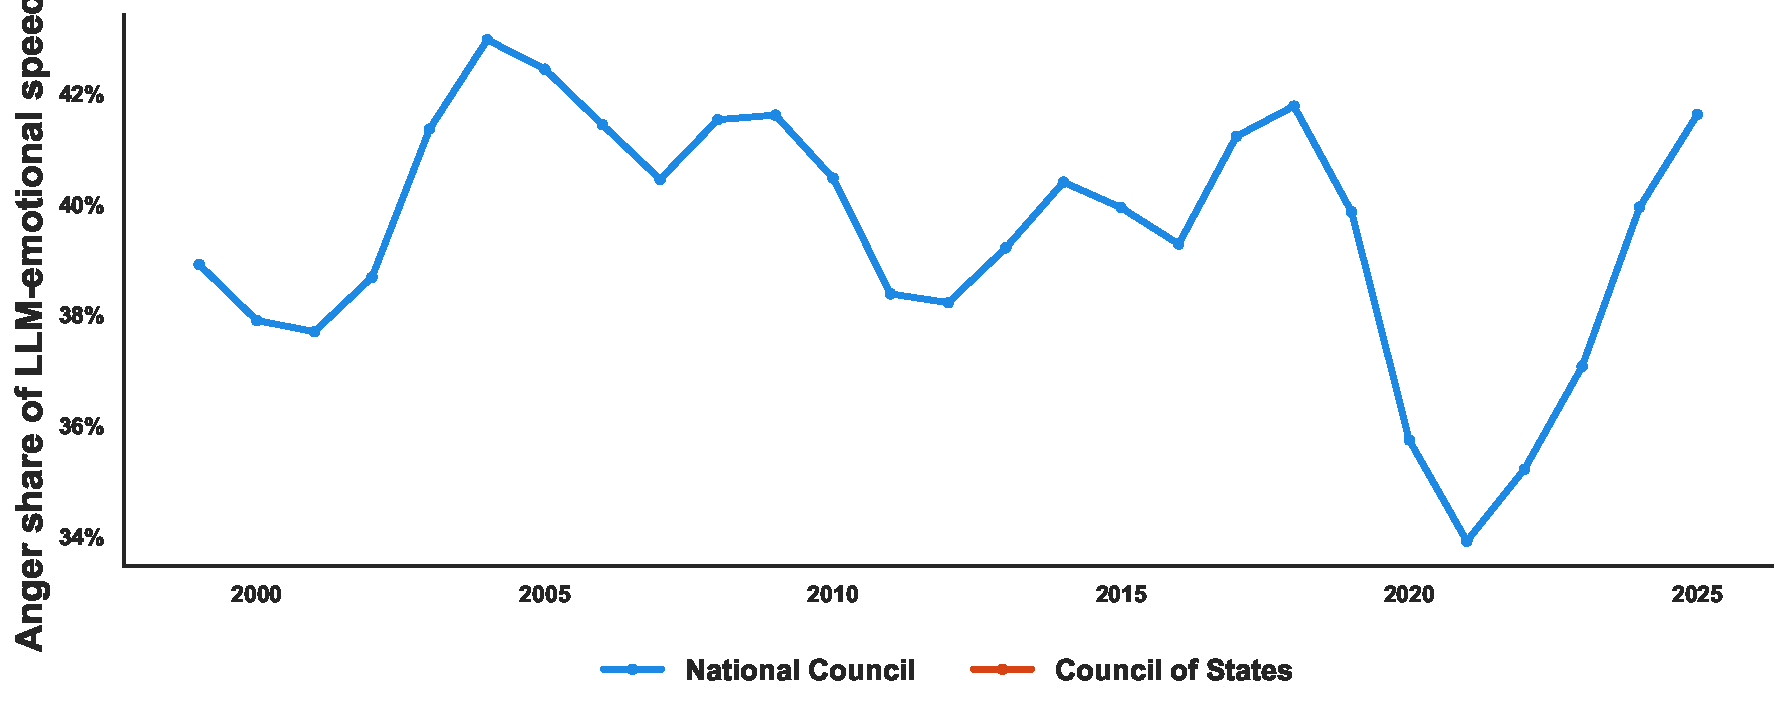
\includegraphics[width=0.82\textwidth,height=0.82\textheight,keepaspectratio]{fig_lt_council_anger.pdf}
    \end{frame}
\begin{frame}{Albert Rösti --- Emotional Rhetoric Before and After Joining the Bundesrat}
\hypertarget{part.FOCUS.roesti}{}
\centering
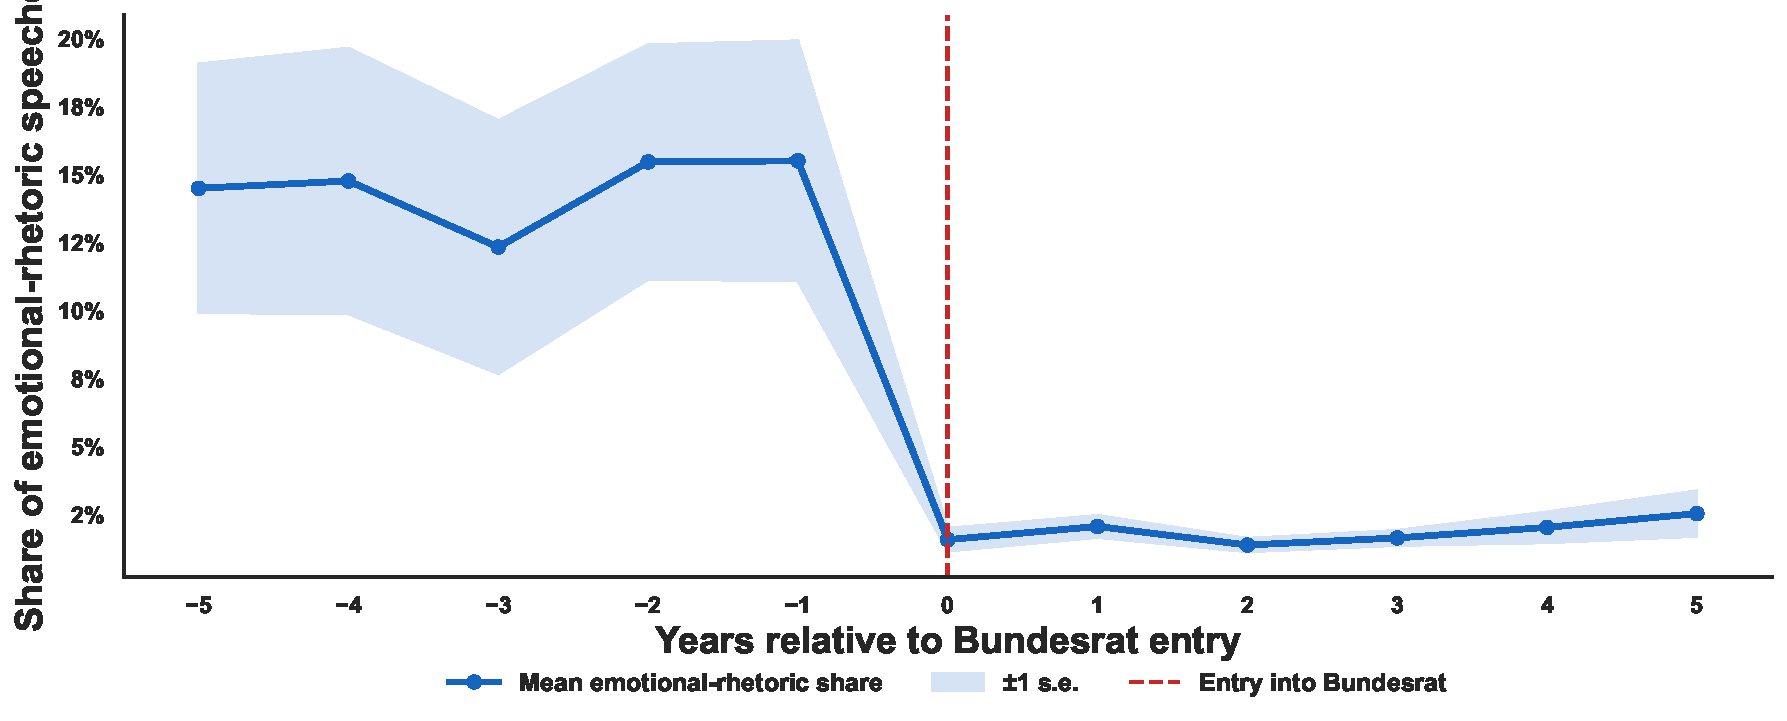
\includegraphics[width=0.86\textwidth,height=0.82\textheight,keepaspectratio]{fig_federal_council_event_emotionality_defD.pdf}
\end{frame}
\begin{frame}{Albert Rösti --- Share of Emotional Speeches}
    \centering
    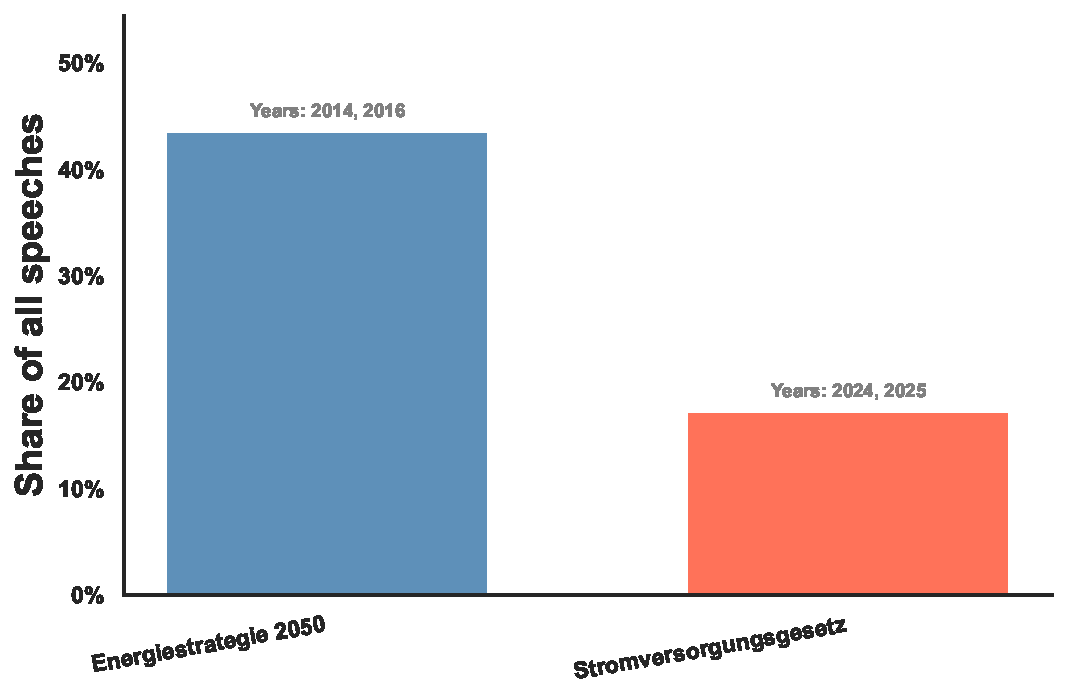
\includegraphics[width=0.82\textwidth,height=0.82\textheight,keepaspectratio]{fig_roesti_energy_emotional_breakdown_defD.pdf}
    \end{frame}
\begin{frame}{Albert Rösti --- Dominant Emotion Share by Business}
    \centering
    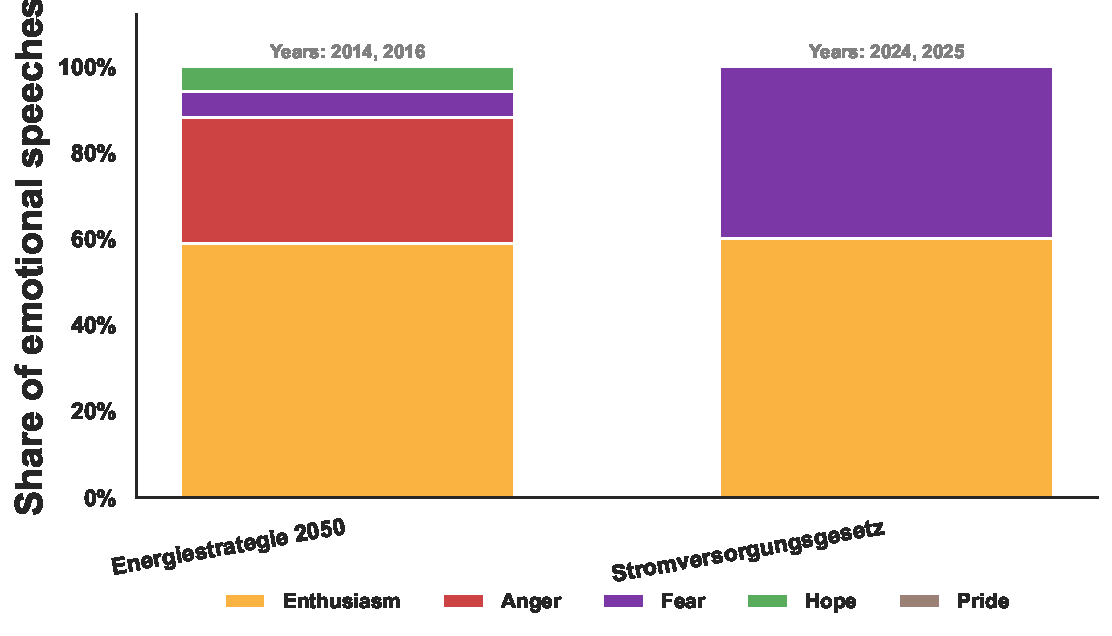
\includegraphics[width=0.88\textwidth,height=0.82\textheight,keepaspectratio]{fig_roesti_emotions_over_time_defD.pdf}
    \end{frame}

\appendix
\section{Appendix}
\begin{frame}{}
\vfill
\centering
\hypertarget{part.APP}{}
{\Large \textbf{Appendix}}\\[0.4cm]
{\normalsize Detailed emotion-by-topic panels and extras}
\vfill
\end{frame}

\begin{frame}{Appendix --- Topic Distribution Over Time --- Ständerat}
\hypertarget{app.SR.topic}{}
\centering
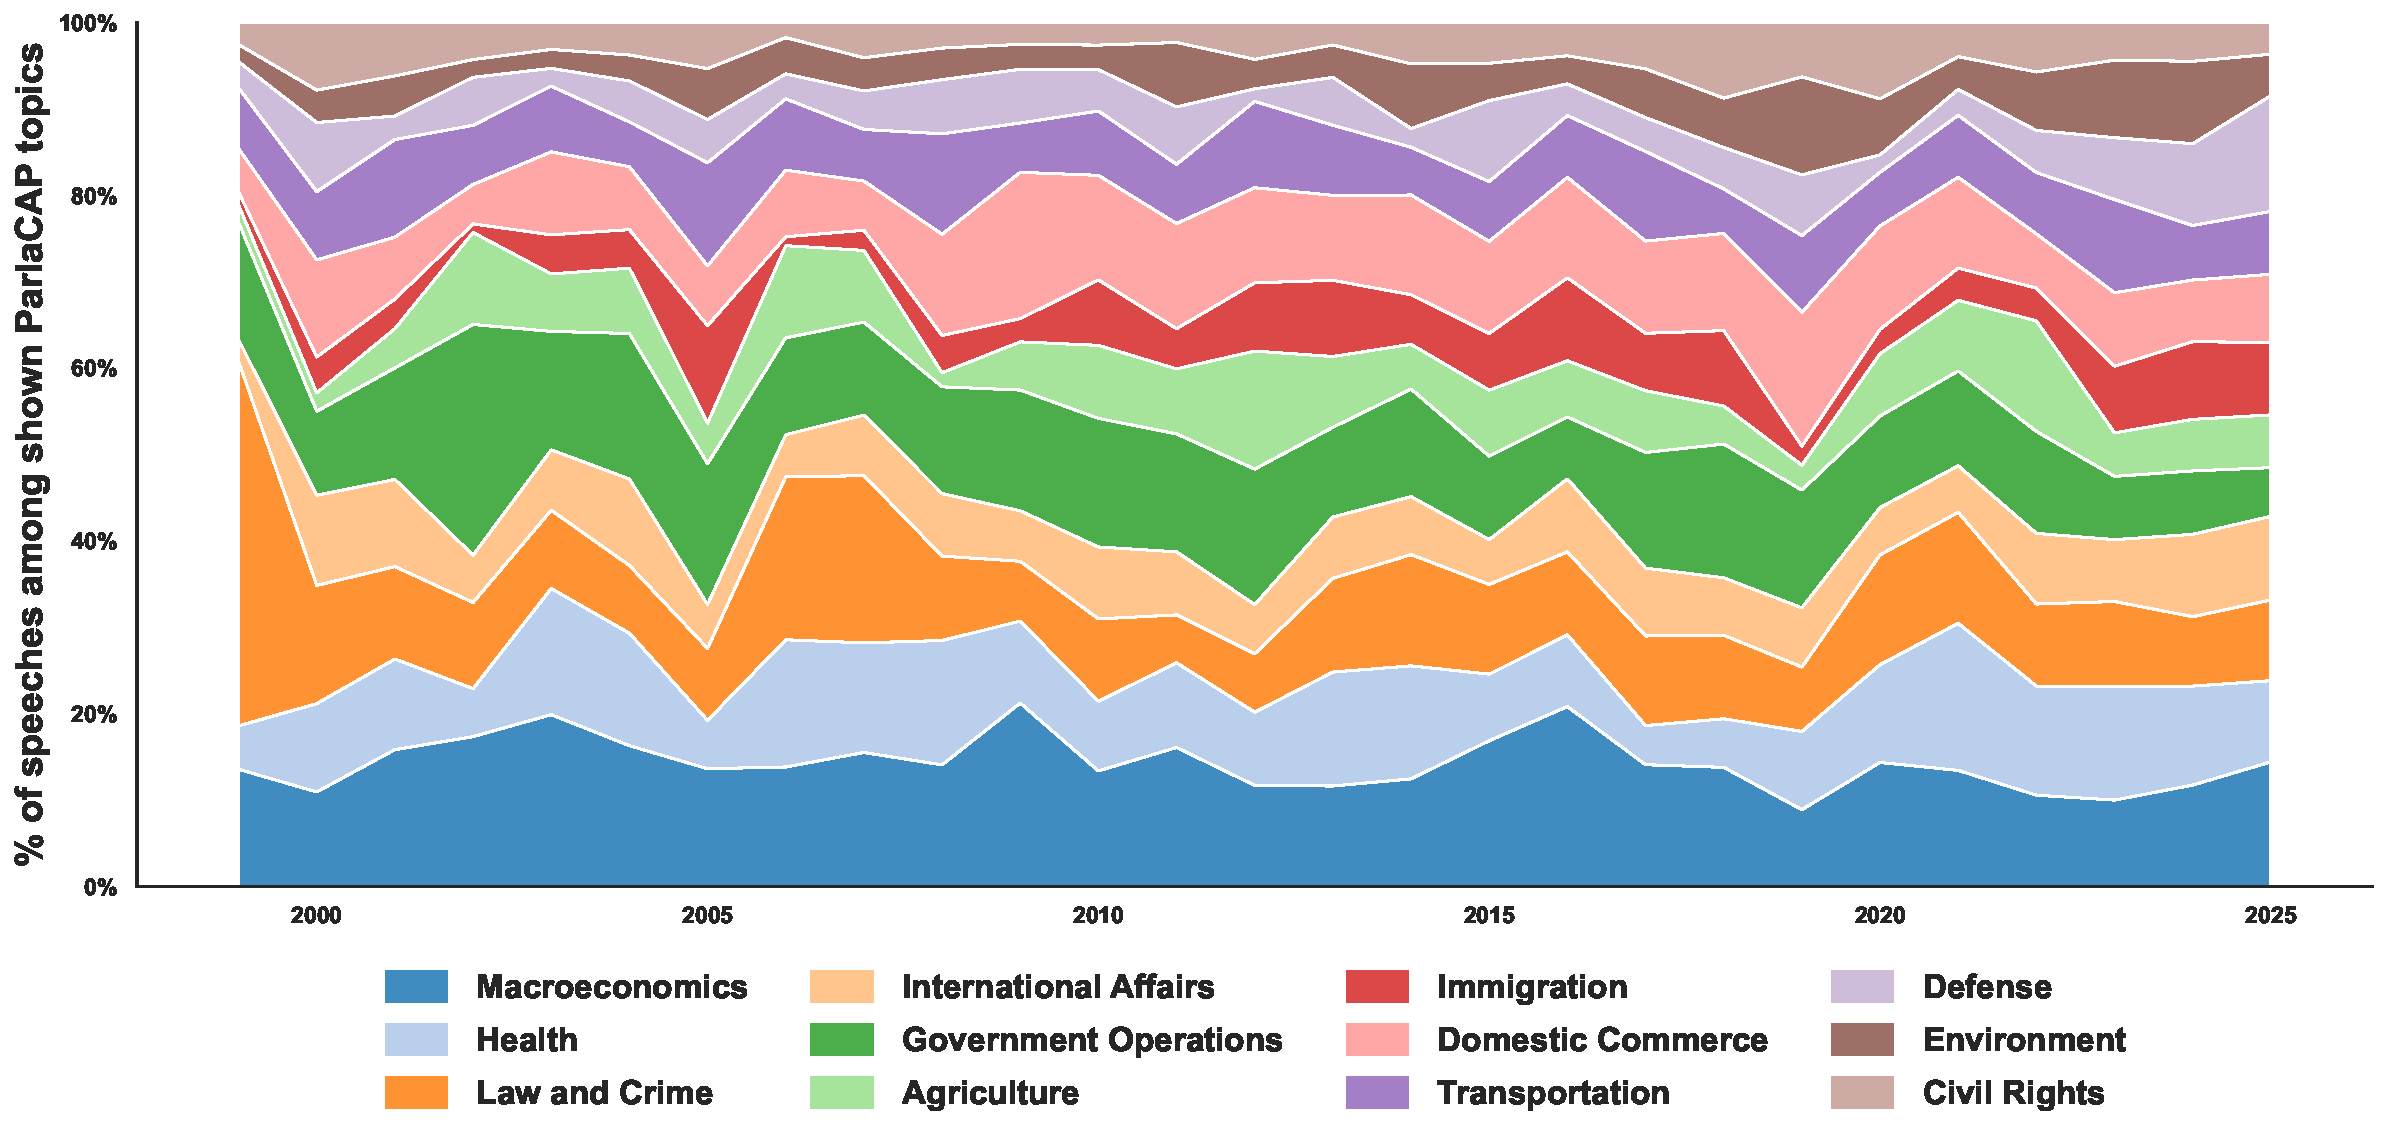
\includegraphics[width=0.97\textwidth,height=0.76\textheight,keepaspectratio]{staenderat_fig_v4_topic_merged9_noproc_stacked.pdf}
\vfill
{\footnotesize\hyperlink{main.SR.topic}{Back to condensed Ständerat topic slide}.}
\end{frame}
\begin{frame}{Appendix --- Aggregated Topic Distribution Over Time --- Ständerat}
    \centering
    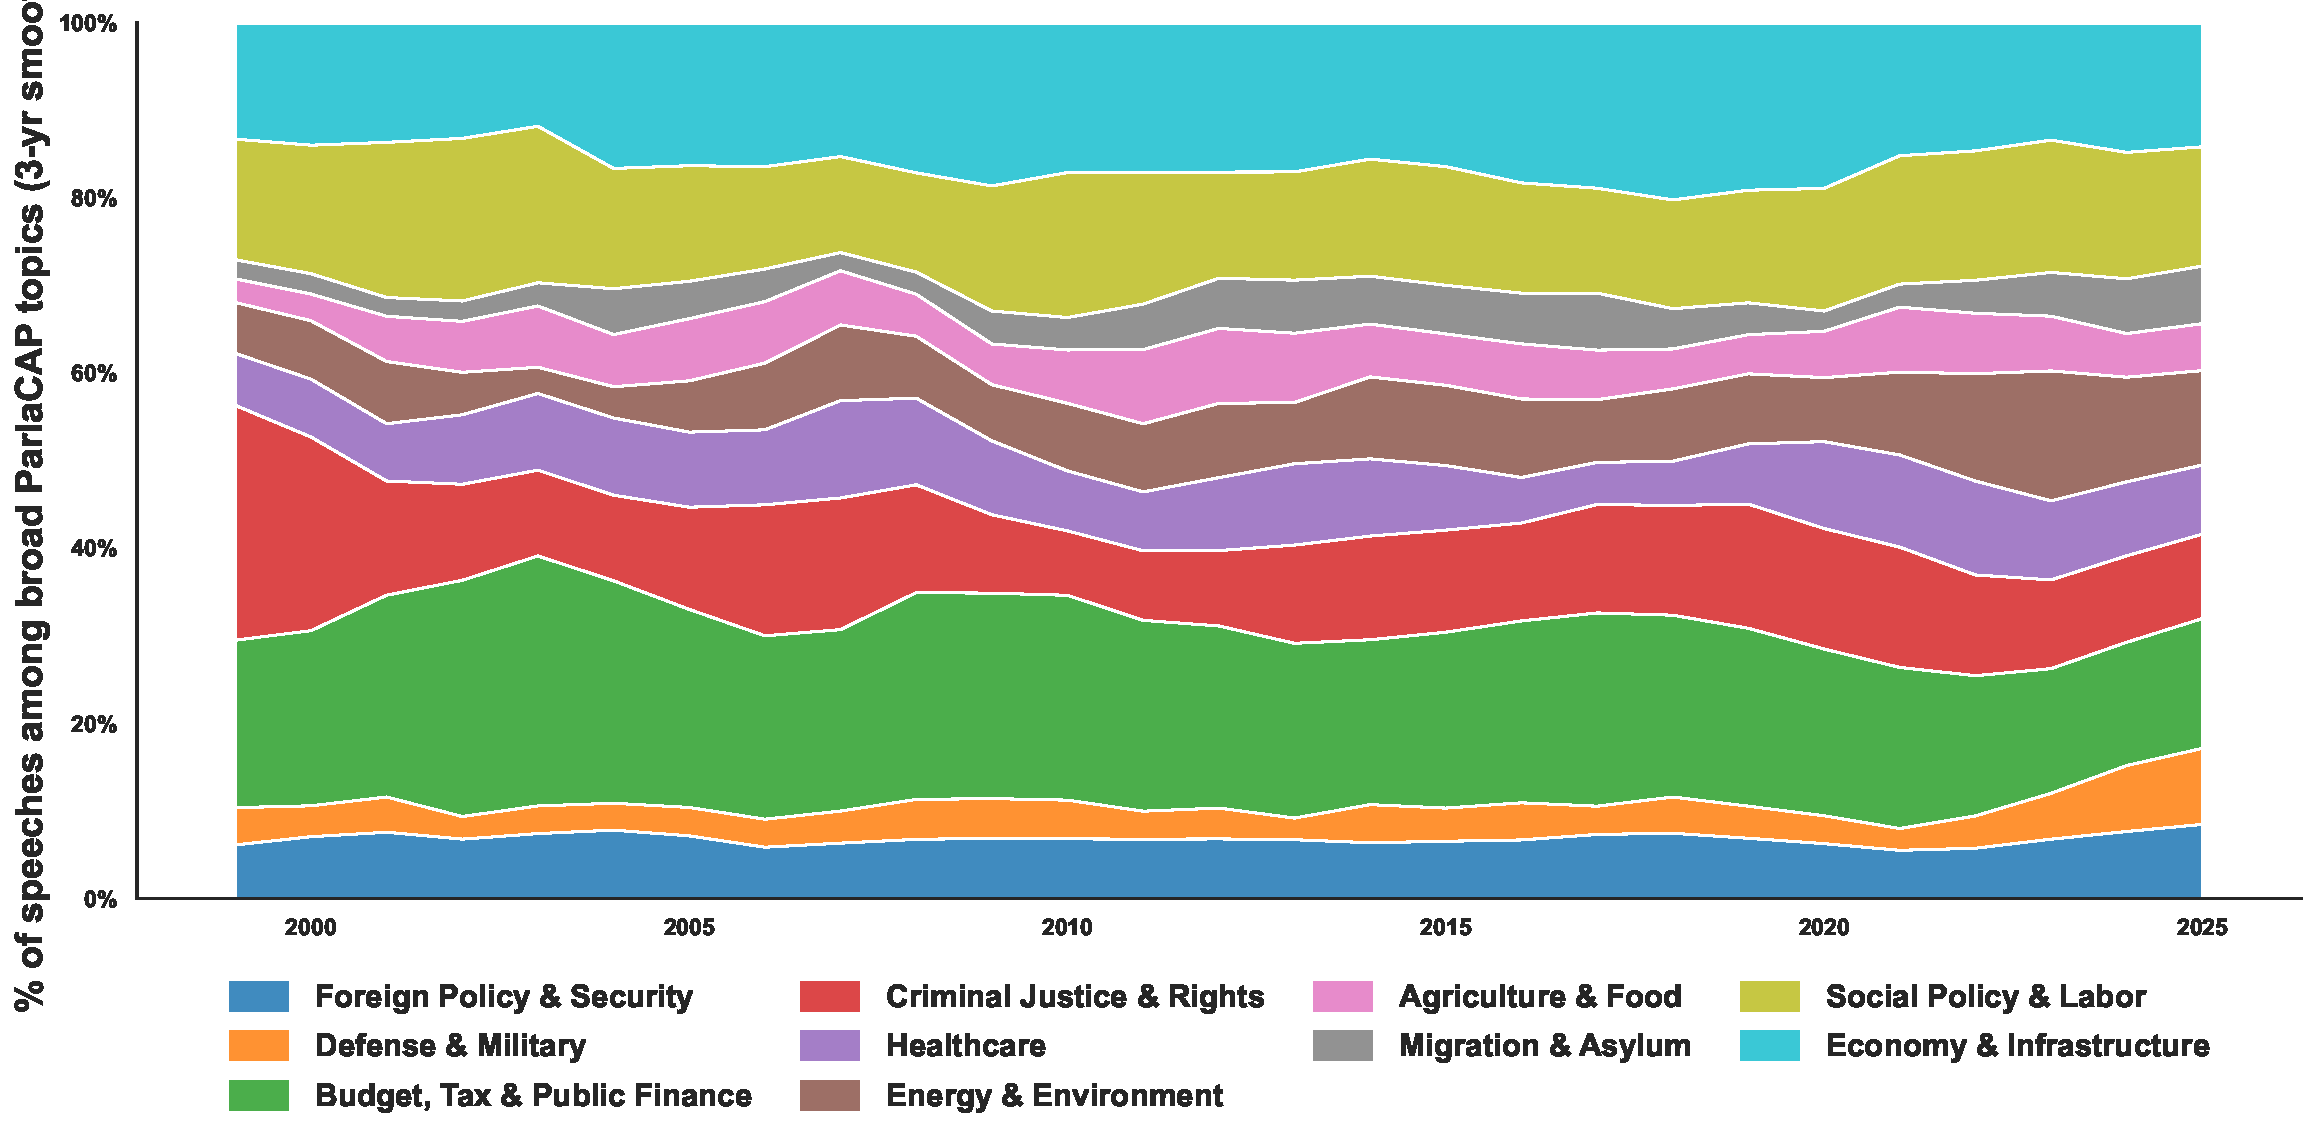
\includegraphics[width=0.97\textwidth,height=0.76\textheight,keepaspectratio]{staenderat_fig_parlacap_broad_topic_stacked_smoothed.pdf}
    \vfill
    {\footnotesize\hyperlink{main.SR.topic}{Back to condensed Ständerat slide}.}
    \end{frame}
\begin{frame}{Appendix --- Topic Emphasis by Party --- Ständerat}
    \centering
    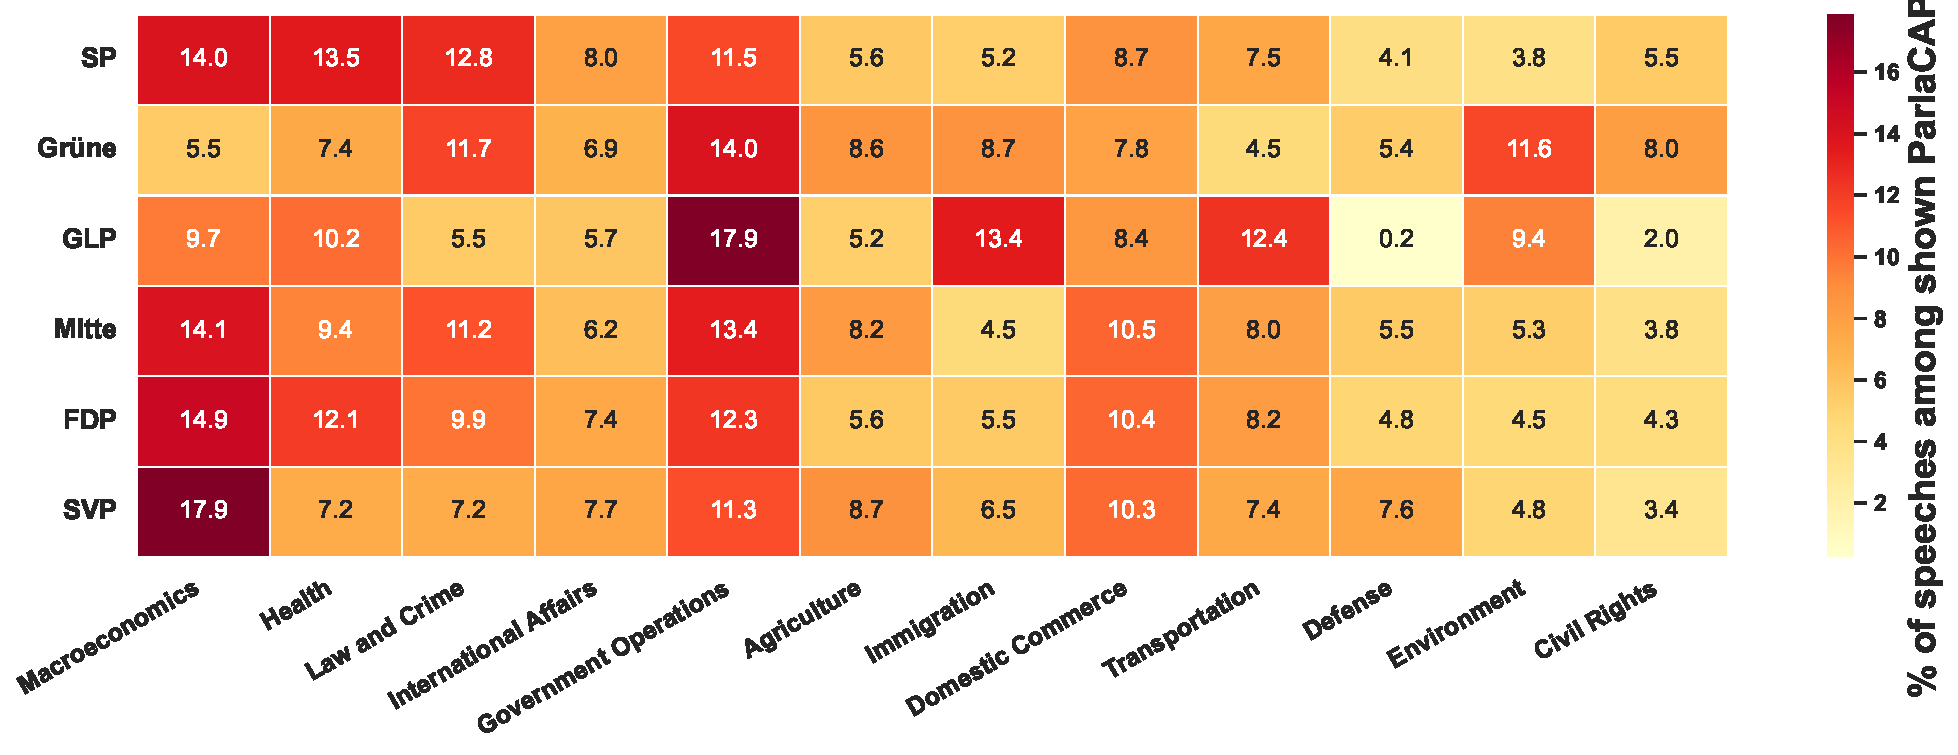
\includegraphics[width=0.94\textwidth,height=0.76\textheight,keepaspectratio]{staenderat_fig_v4_topic_merged_party_noproc.pdf}
    \vfill
    {\footnotesize\hyperlink{main.SR.topic}{Back to condensed Ständerat slide}.}
    \end{frame}
\begin{frame}{Appendix --- Relative Shift in Parliamentary Attention --- Ständerat}
    \centering
    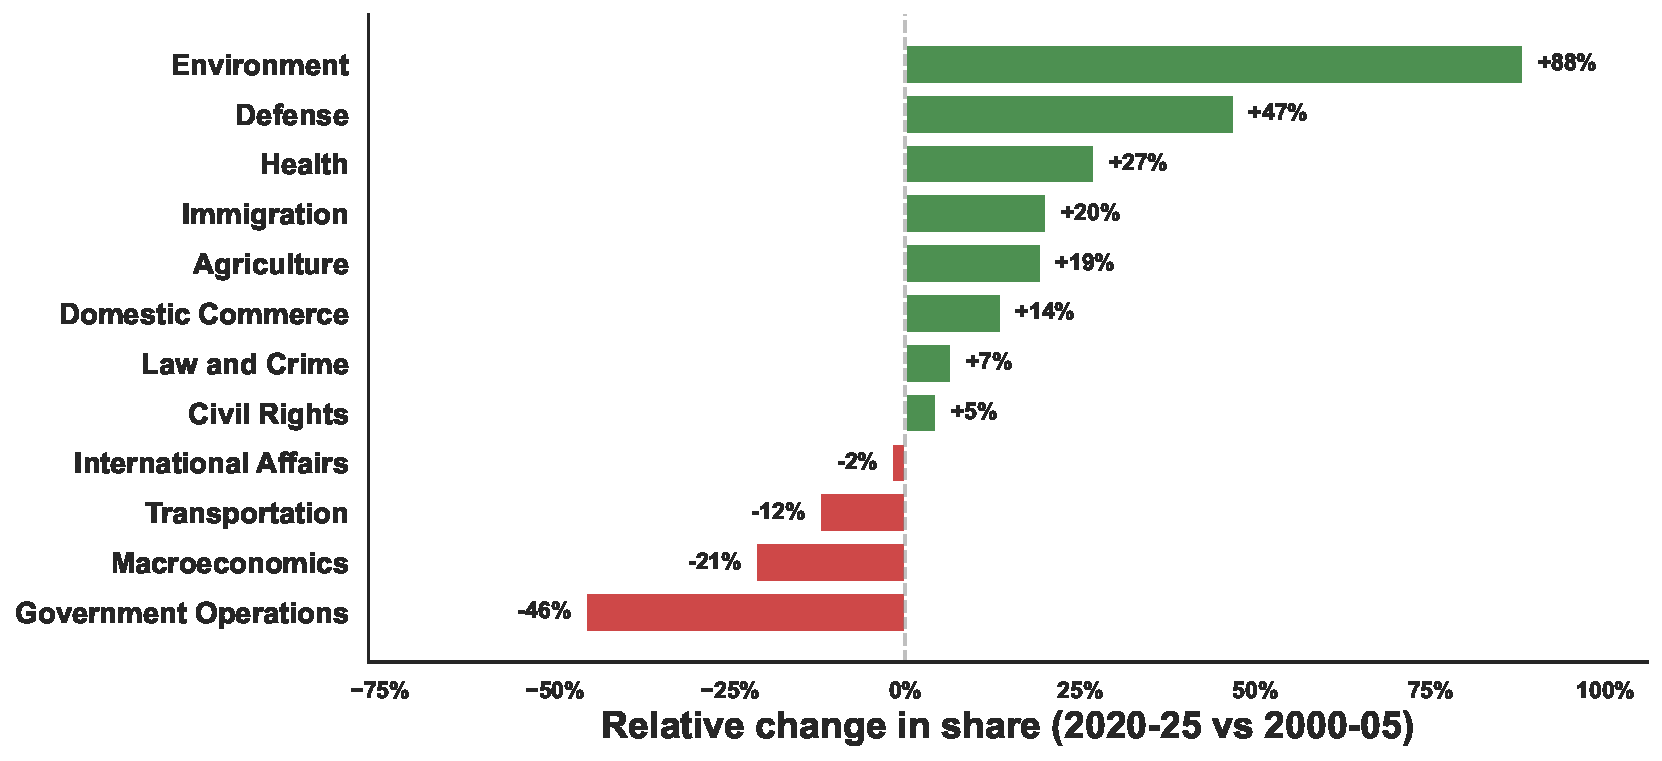
\includegraphics[width=0.82\textwidth,height=0.76\textheight,keepaspectratio]{staenderat_fig_lt_topic_shift_proportion.pdf}
    \vfill
    {\footnotesize\hyperlink{main.SR.topic}{Back to condensed Ständerat slide}.}
    \end{frame}
\begin{frame}{Appendix --- Who Drives Topic Shifts? --- Ständerat}
    \centering
    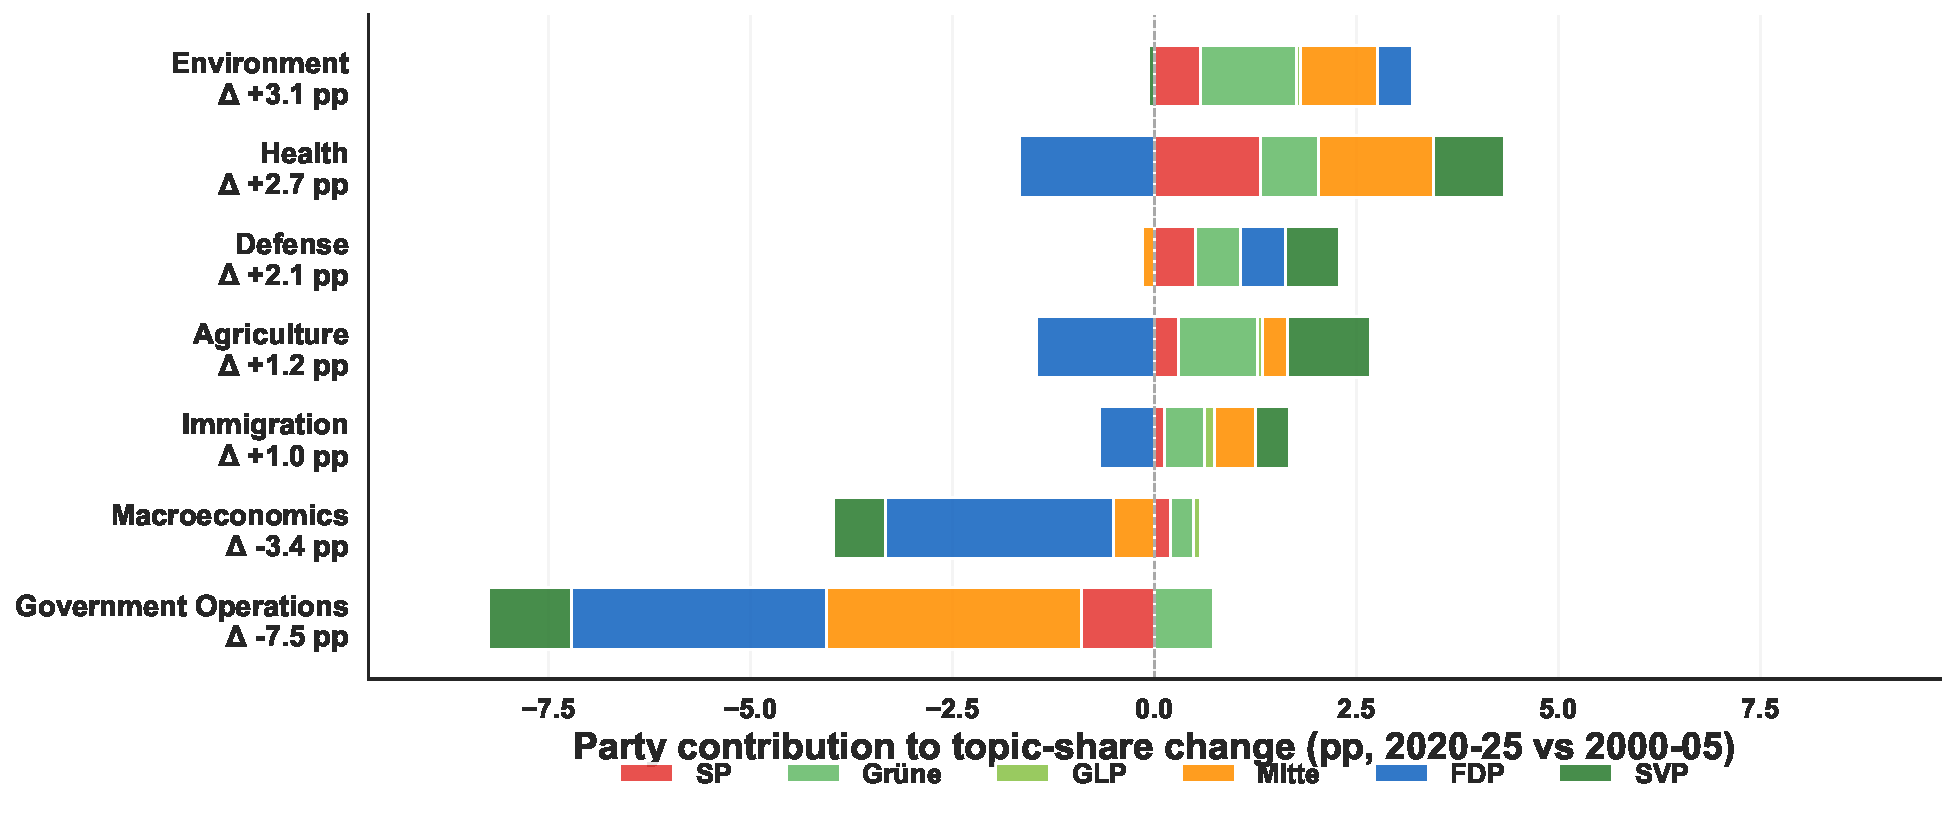
\includegraphics[width=0.88\textwidth,height=0.76\textheight,keepaspectratio]{staenderat_fig_topic_shift_drivers_by_party.pdf}
    \vfill
    {\footnotesize\hyperlink{main.SR.topic}{Back to condensed Ständerat slide}.}
    \end{frame}

\begin{frame}{Appendix --- Emotional Rhetoric by Party --- Ständerat}
\hypertarget{app.SR.emotion}{}
\centering
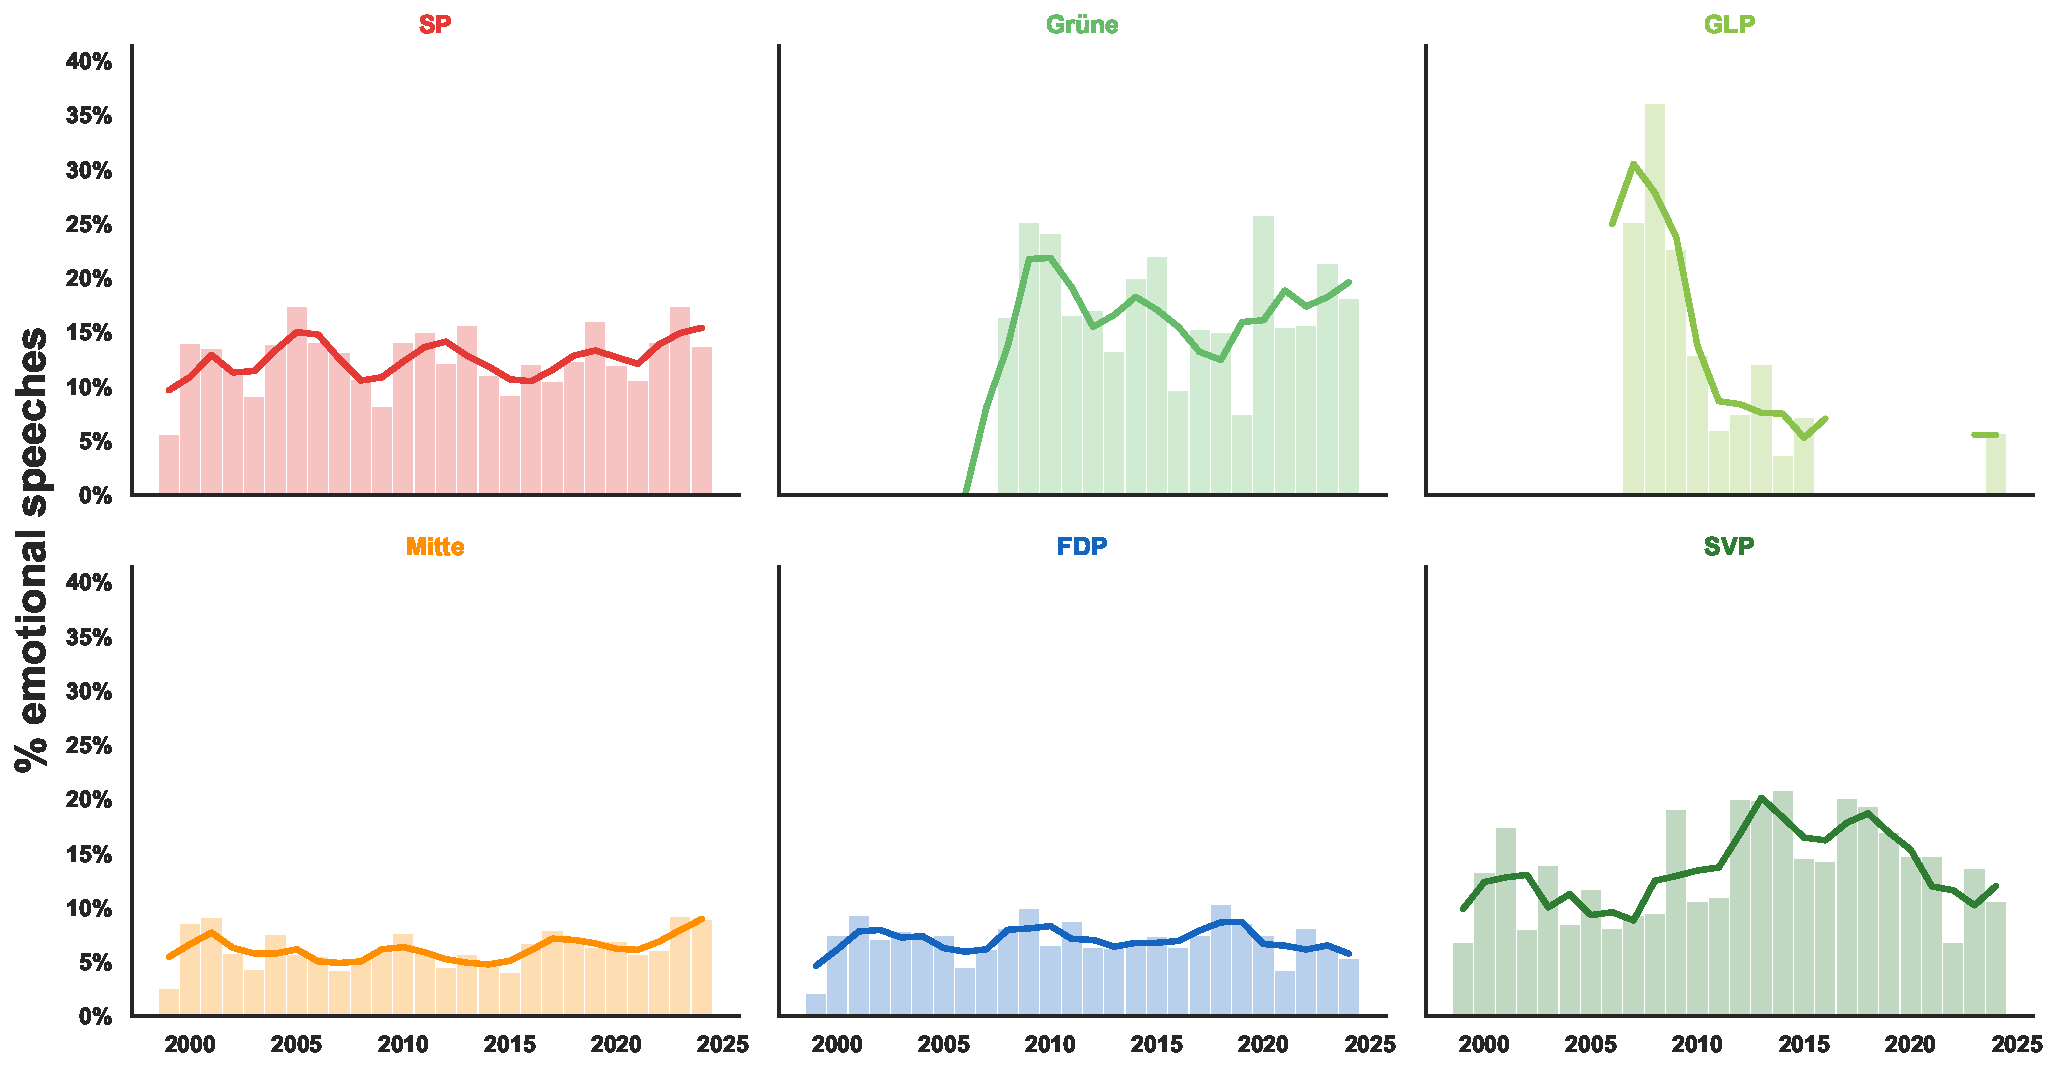
\includegraphics[width=0.92\textwidth,height=0.76\textheight,keepaspectratio]{staenderat_fig_lt_defD_by_party.pdf}
\vfill
{\footnotesize\hyperlink{main.SR.emotion}{Back to condensed Ständerat emotion slide}.}
\end{frame}
\begin{frame}{Appendix --- Emotional Rhetoric by Legislature and Party --- Ständerat}
\centering
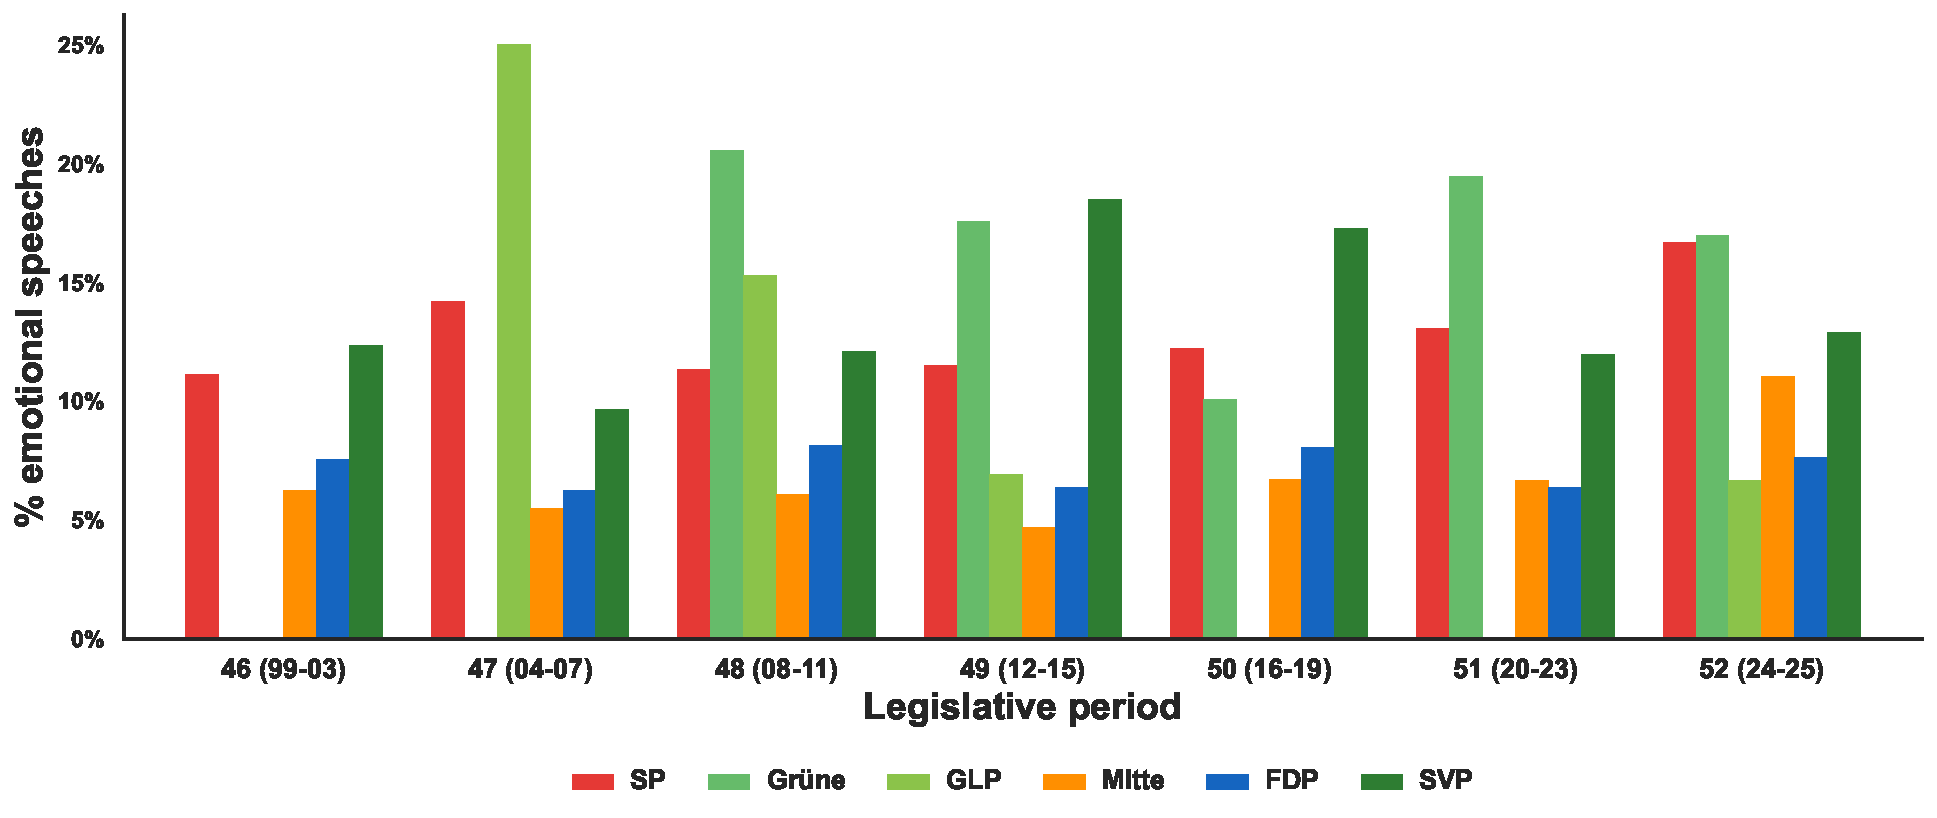
\includegraphics[width=0.93\textwidth,height=0.74\textheight,keepaspectratio]{staenderat_fig_lt_defD_by_legislature.pdf}
\vfill
{\footnotesize\textit{Note:} Same legislature boundaries as for the National Council (October federal elections). GLP (PVL) entered with the 2007 election; there is no 47th-period bar for GLP. \hyperlink{main.SR.emotion}{Back to condensed Ständerat emotion slide}.}
\end{frame}
\begin{frame}{Appendix --- Emotional Rhetoric Score --- Ständerat}
    \centering
    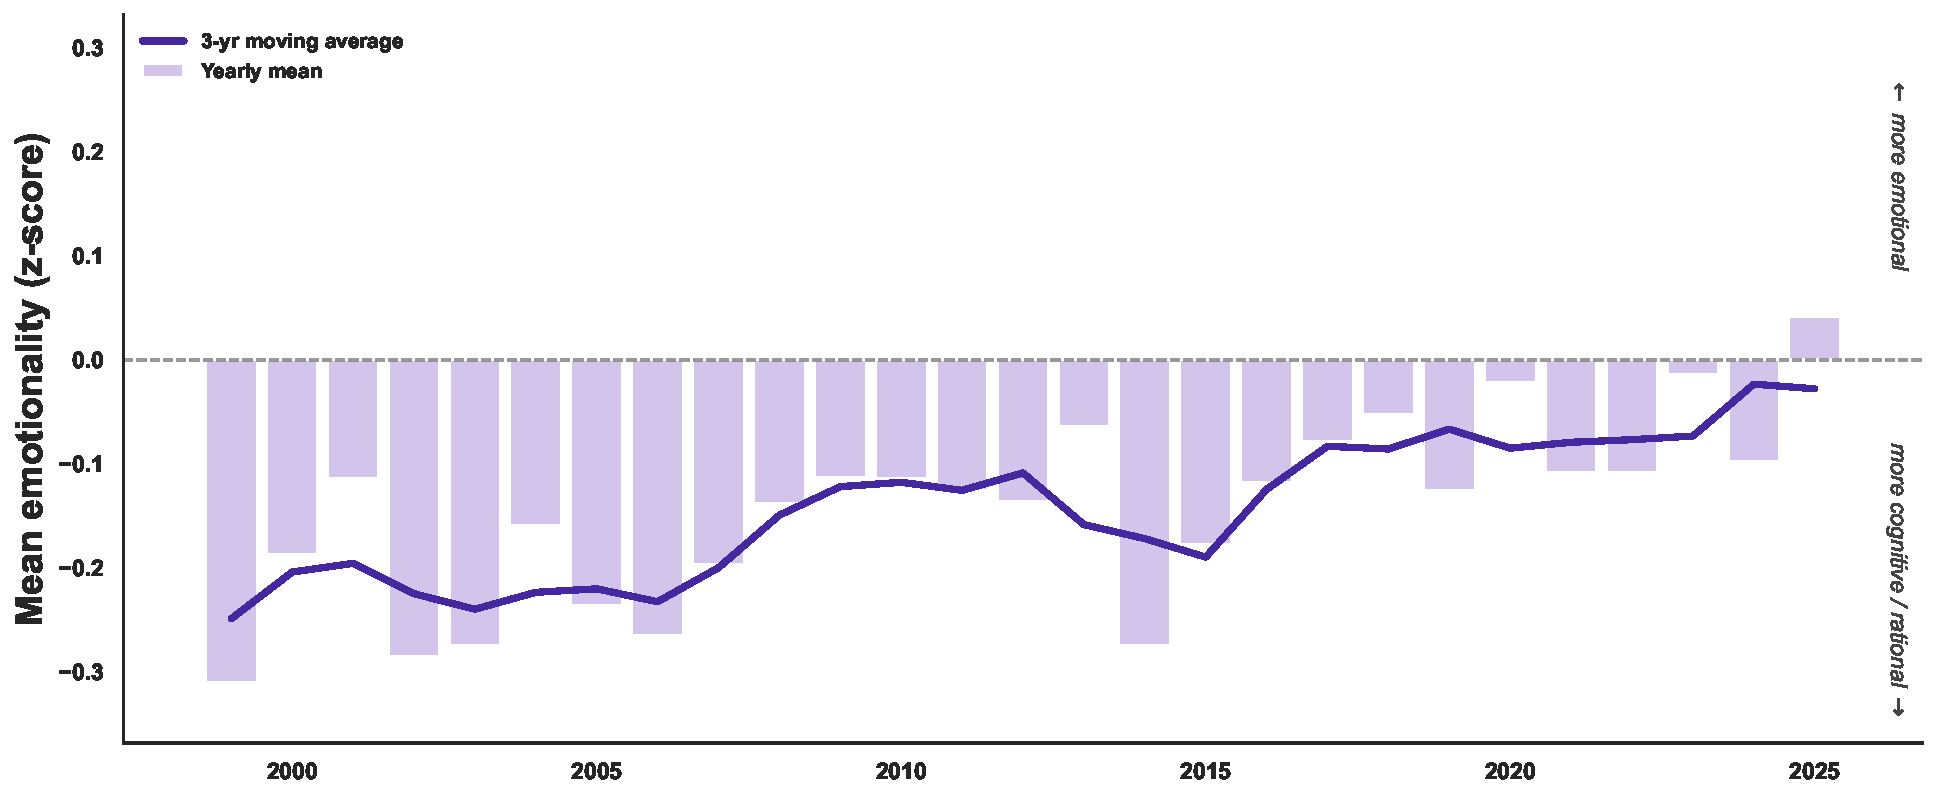
\includegraphics[width=0.90\textwidth,height=0.76\textheight,keepaspectratio]{staenderat_fig_lt_ga_emotionality_time.pdf}
    \vfill
    {\footnotesize\hyperlink{main.SR.emotion}{Back to condensed Ständerat slide}.}
    \end{frame}
\begin{frame}{Appendix --- Emotional Rhetoric Score by Party --- Ständerat}
    \centering
    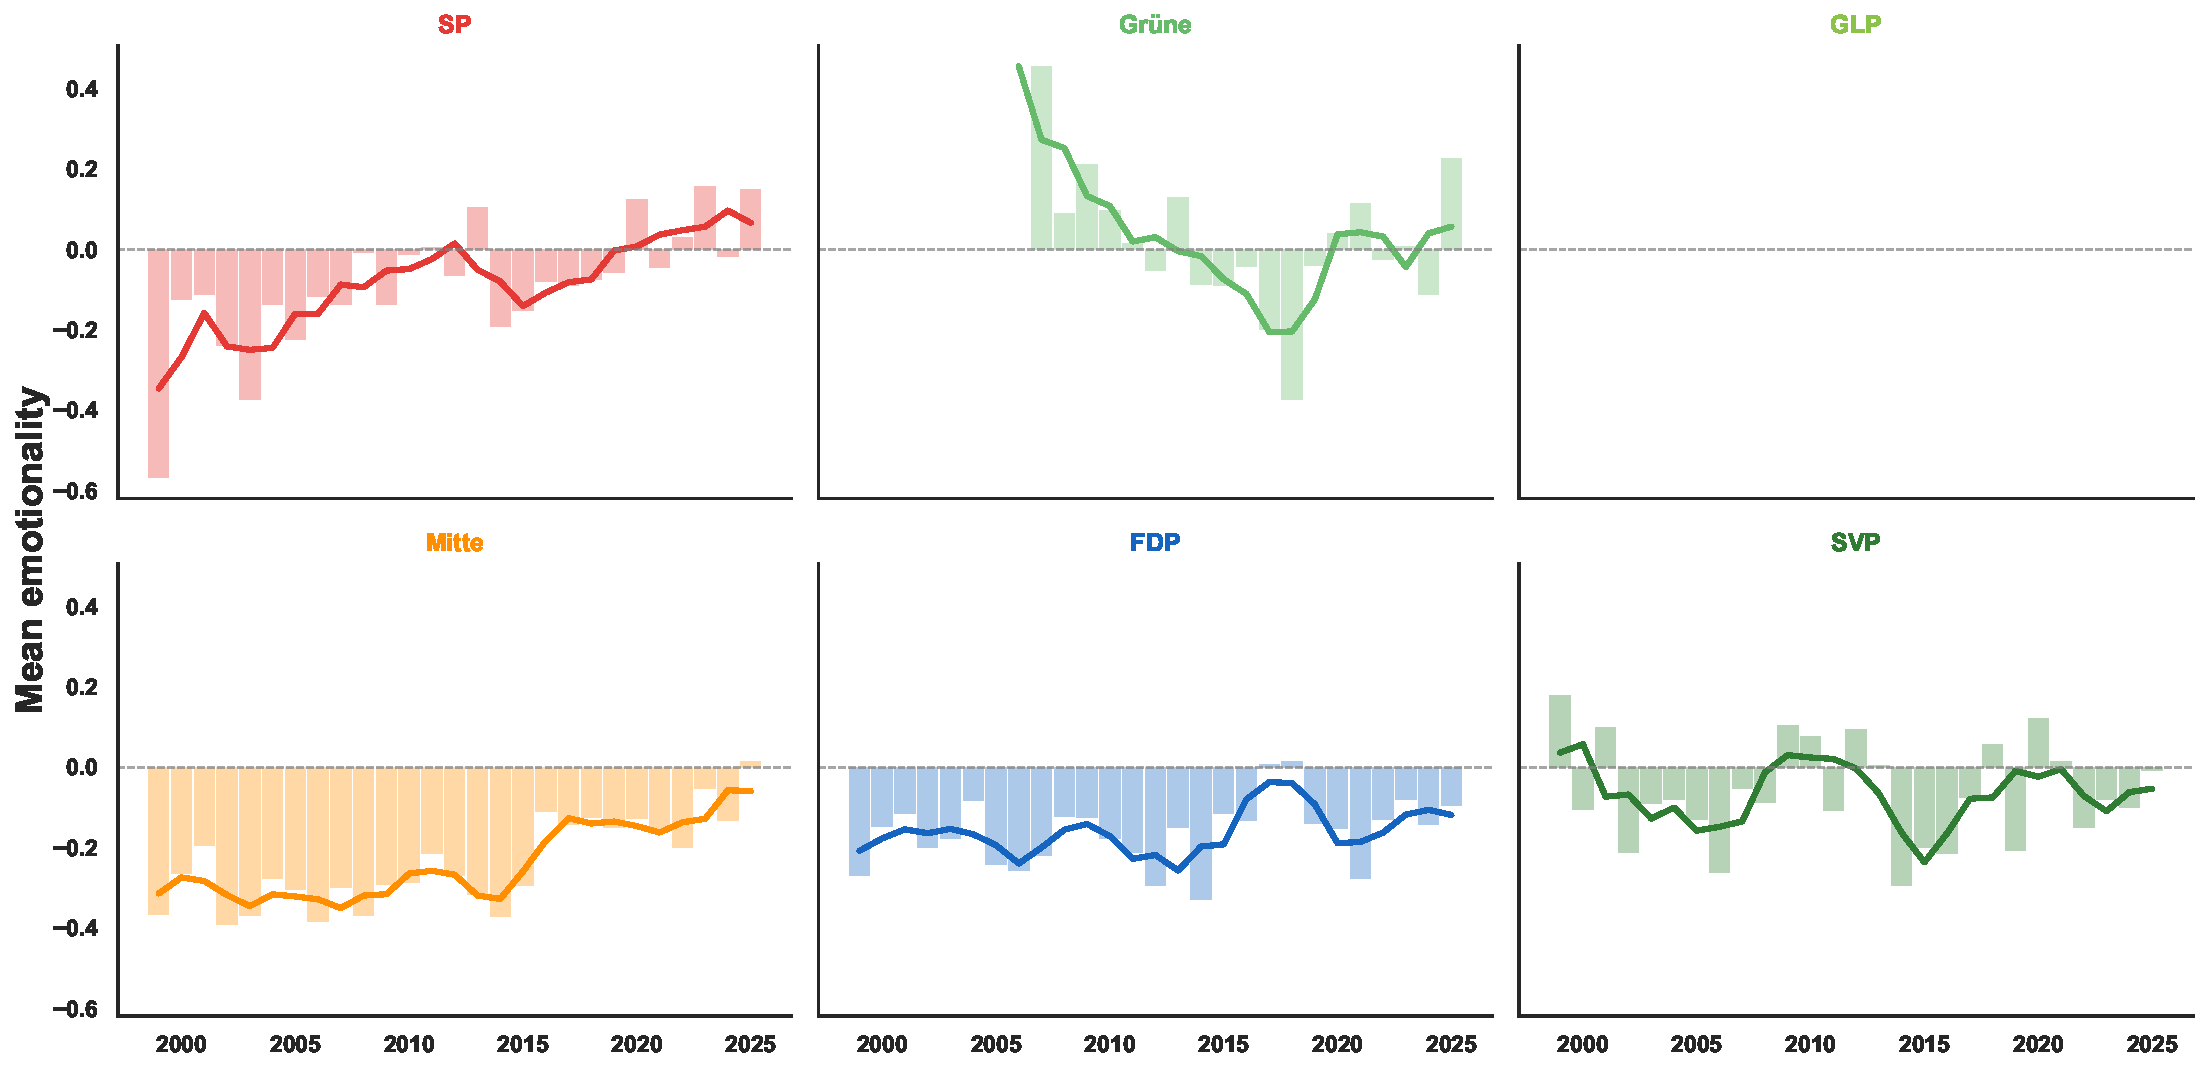
\includegraphics[width=0.92\textwidth,height=0.76\textheight,keepaspectratio]{staenderat_fig_lt_ga_emotionality_party_facet.pdf}
    \vfill
    {\footnotesize\hyperlink{main.SR.emotion}{Back to condensed Ständerat slide}.}
    \end{frame}
\begin{frame}{Appendix --- Emotional Rhetoric Baseline Index --- Ständerat}
    \centering
    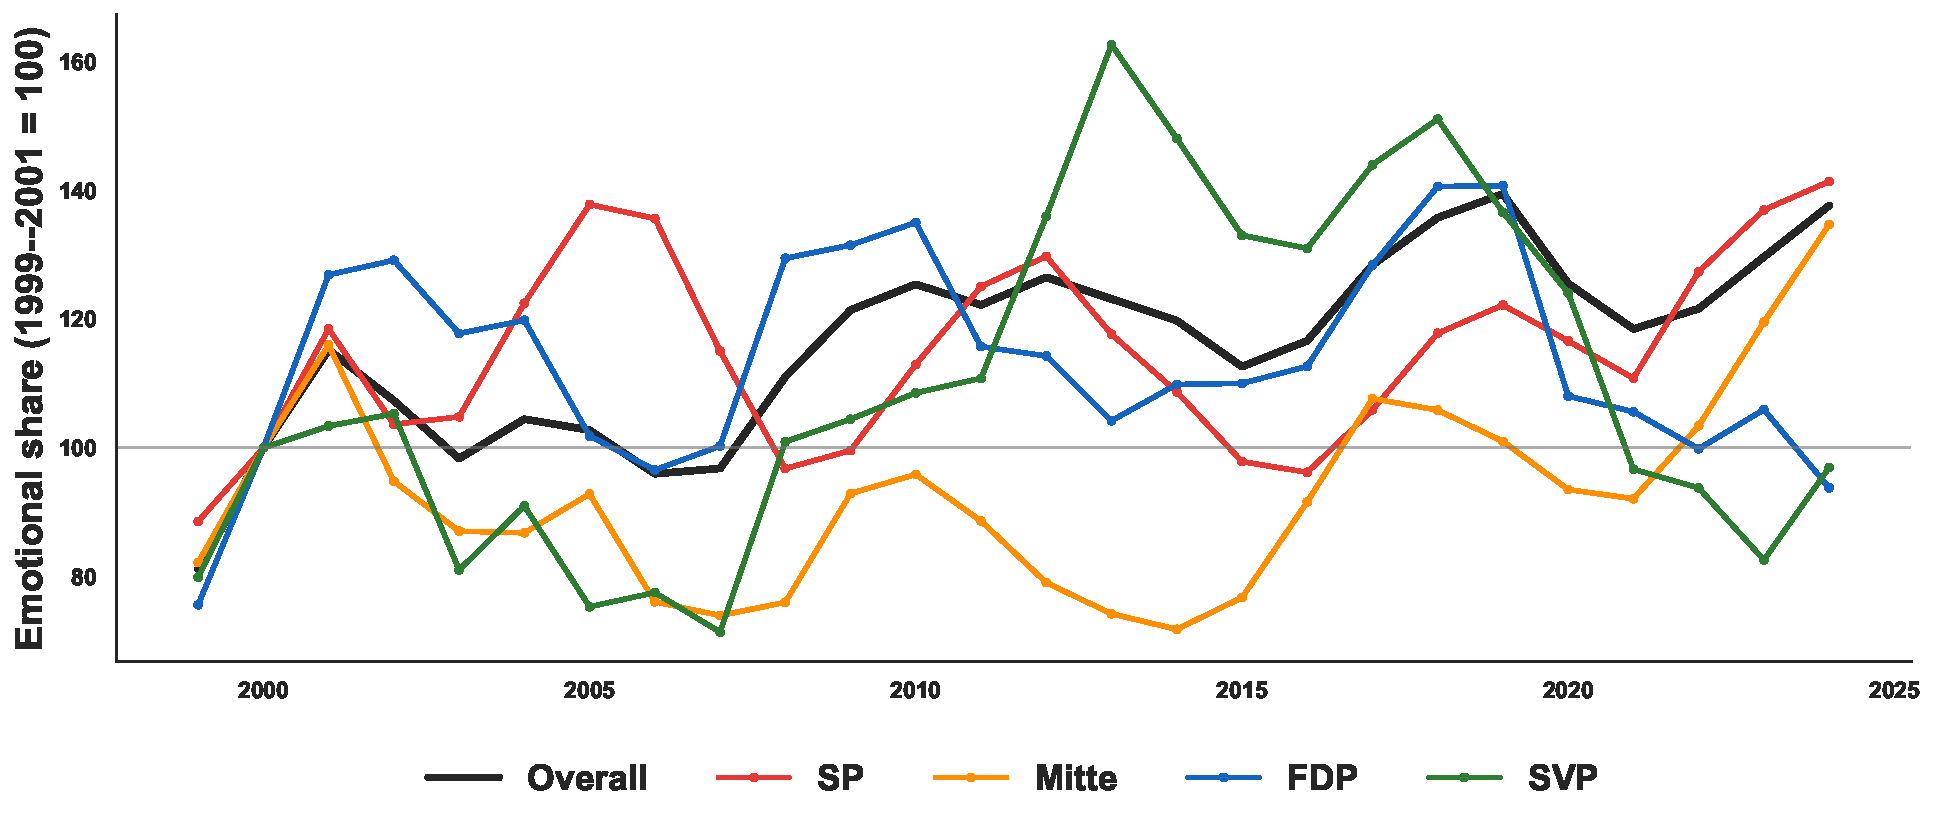
\includegraphics[width=0.86\textwidth,height=0.76\textheight,keepaspectratio]{staenderat_fig_lt_llm_emo_index100.pdf}
    \vfill
    {\footnotesize\hyperlink{main.SR.emotion}{Back to condensed Ständerat slide}.}
    \end{frame}
\begin{frame}{Appendix --- Emotional Rhetoric by Topic --- Ständerat}
    \centering
    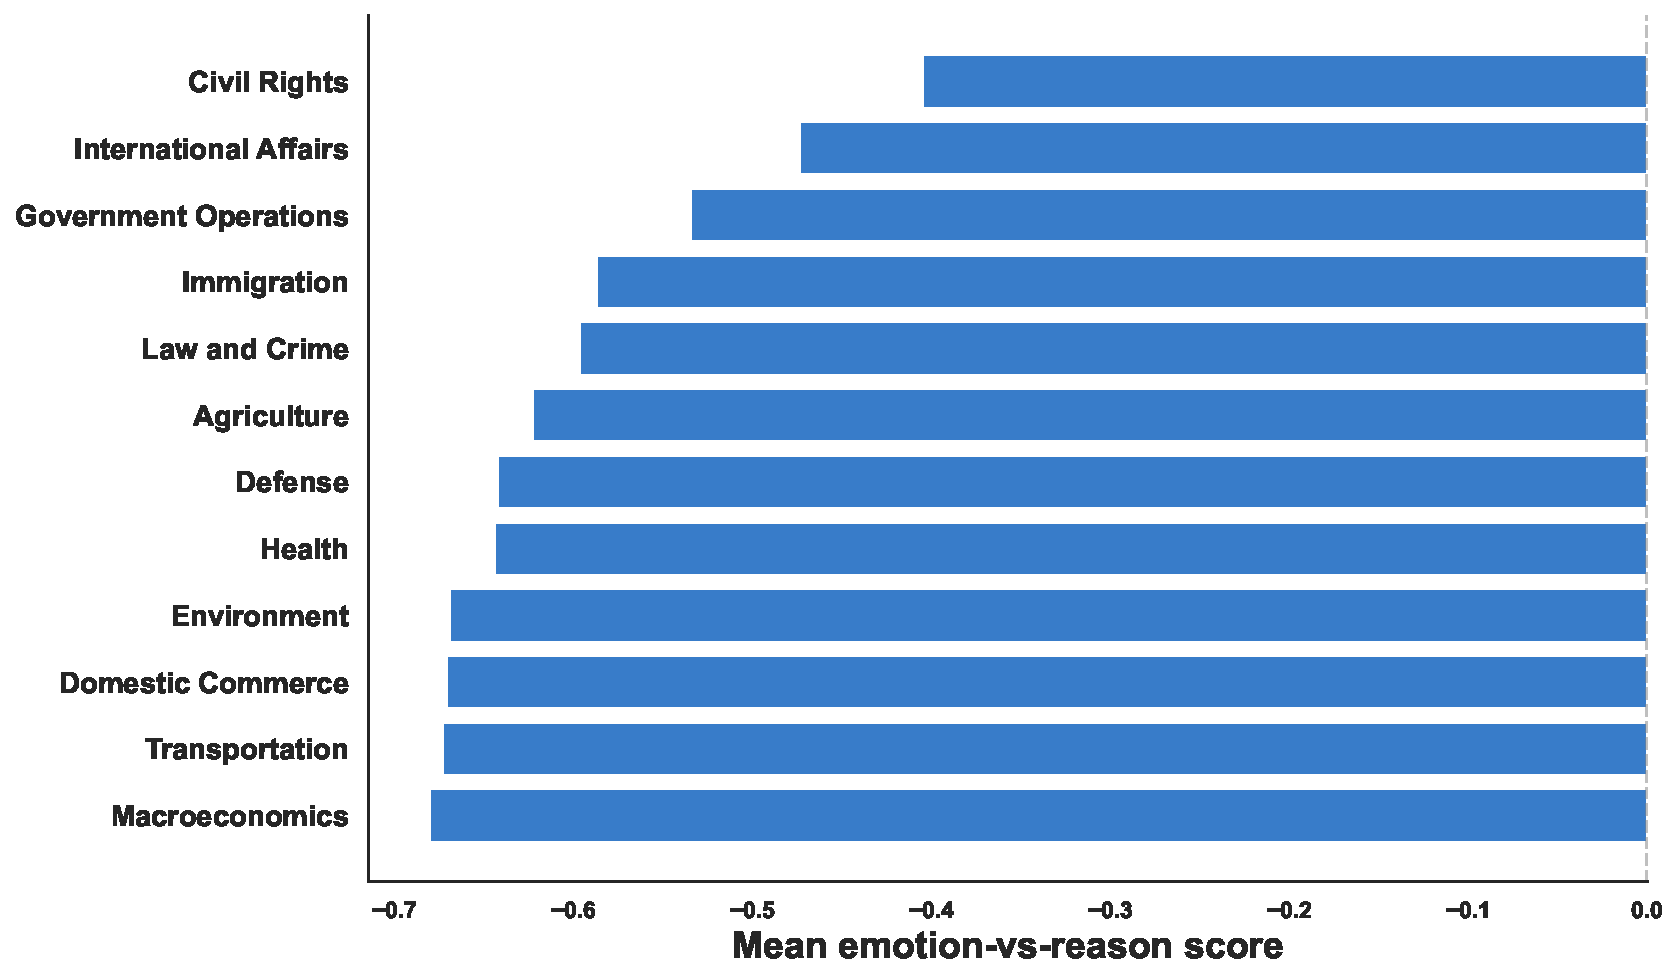
\includegraphics[width=0.78\textwidth,height=0.76\textheight,keepaspectratio]{staenderat_fig_lt_emotionality_topic_large.pdf}
    \vfill
    {\footnotesize\hyperlink{main.SR.emotion}{Back to condensed Ständerat slide}.}
    \end{frame}
\begin{frame}{Appendix --- Emotional Rhetoric Gap by Topic (SVP vs SP) --- Ständerat}
    \centering
    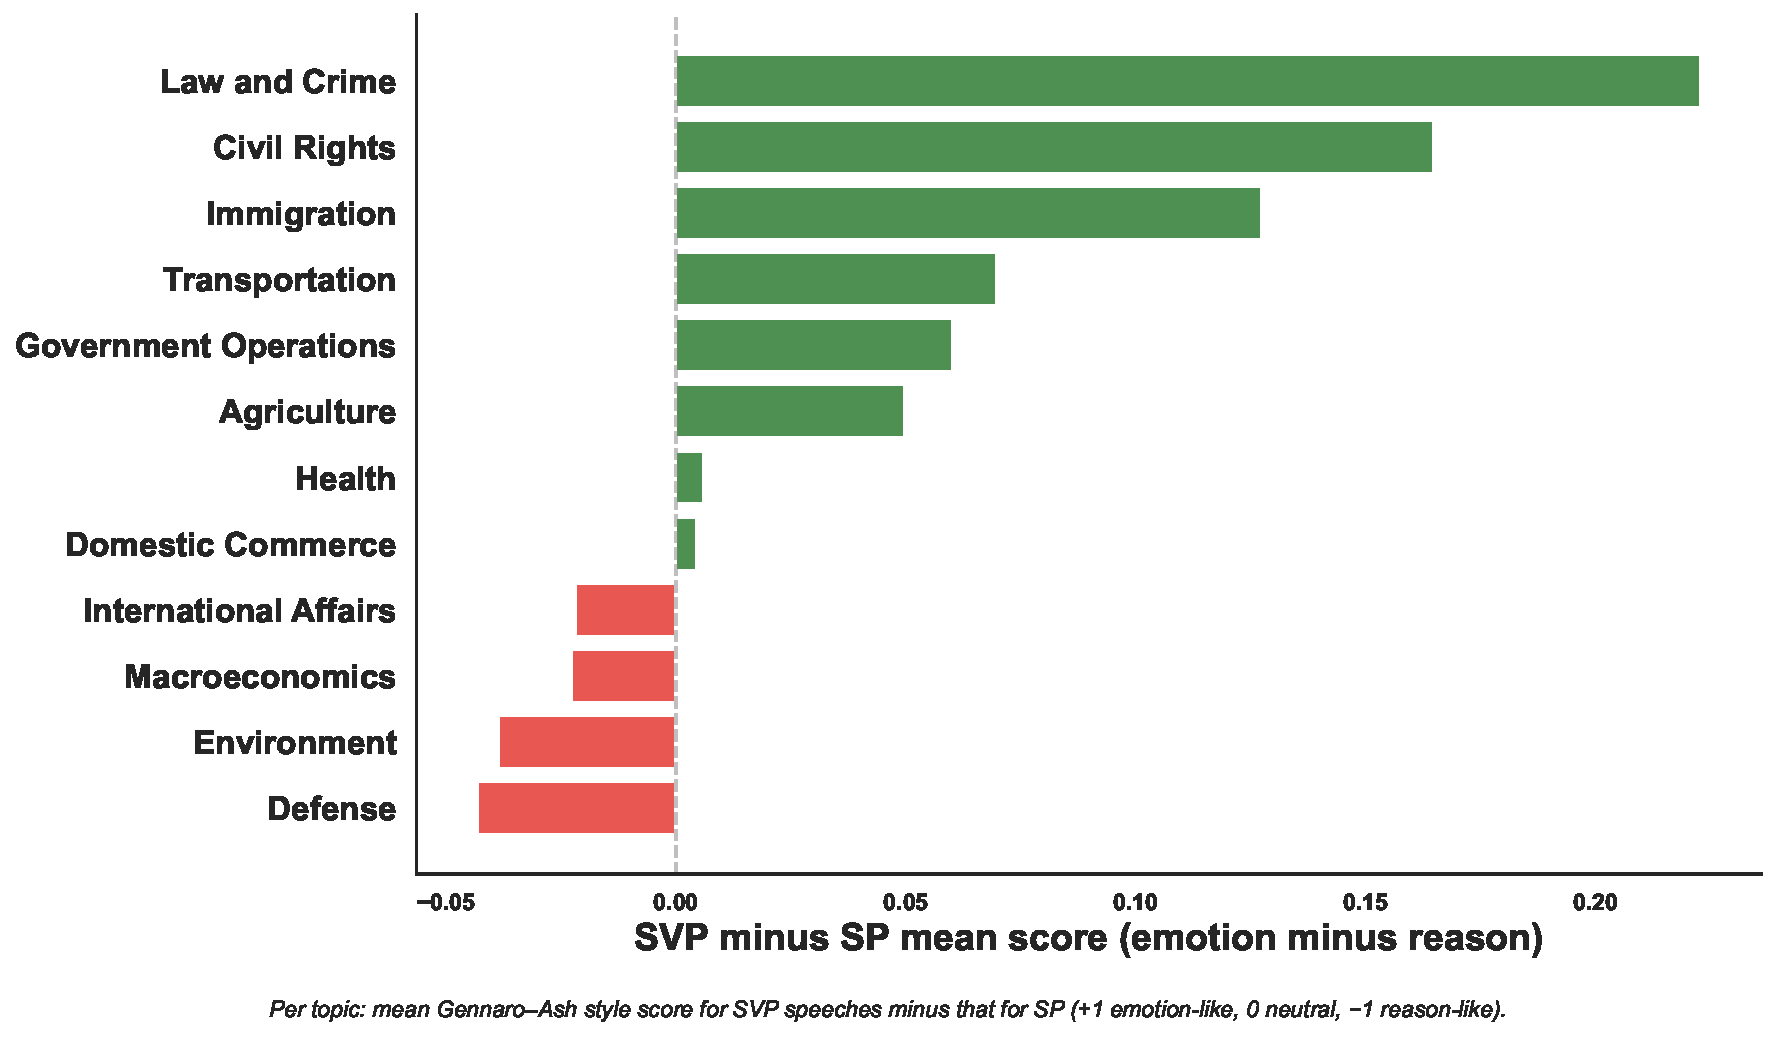
\includegraphics[width=0.72\textwidth,height=0.76\textheight,keepaspectratio]{staenderat_fig_GA_party_ratio_by_topic.pdf}
    \vfill
    {\footnotesize\hyperlink{main.SR.emotion}{Back to condensed Ständerat slide}.}
    \end{frame}
\begin{frame}{Appendix --- Emotional Rhetoric by Topic --- Shift --- Ständerat}
    \centering
    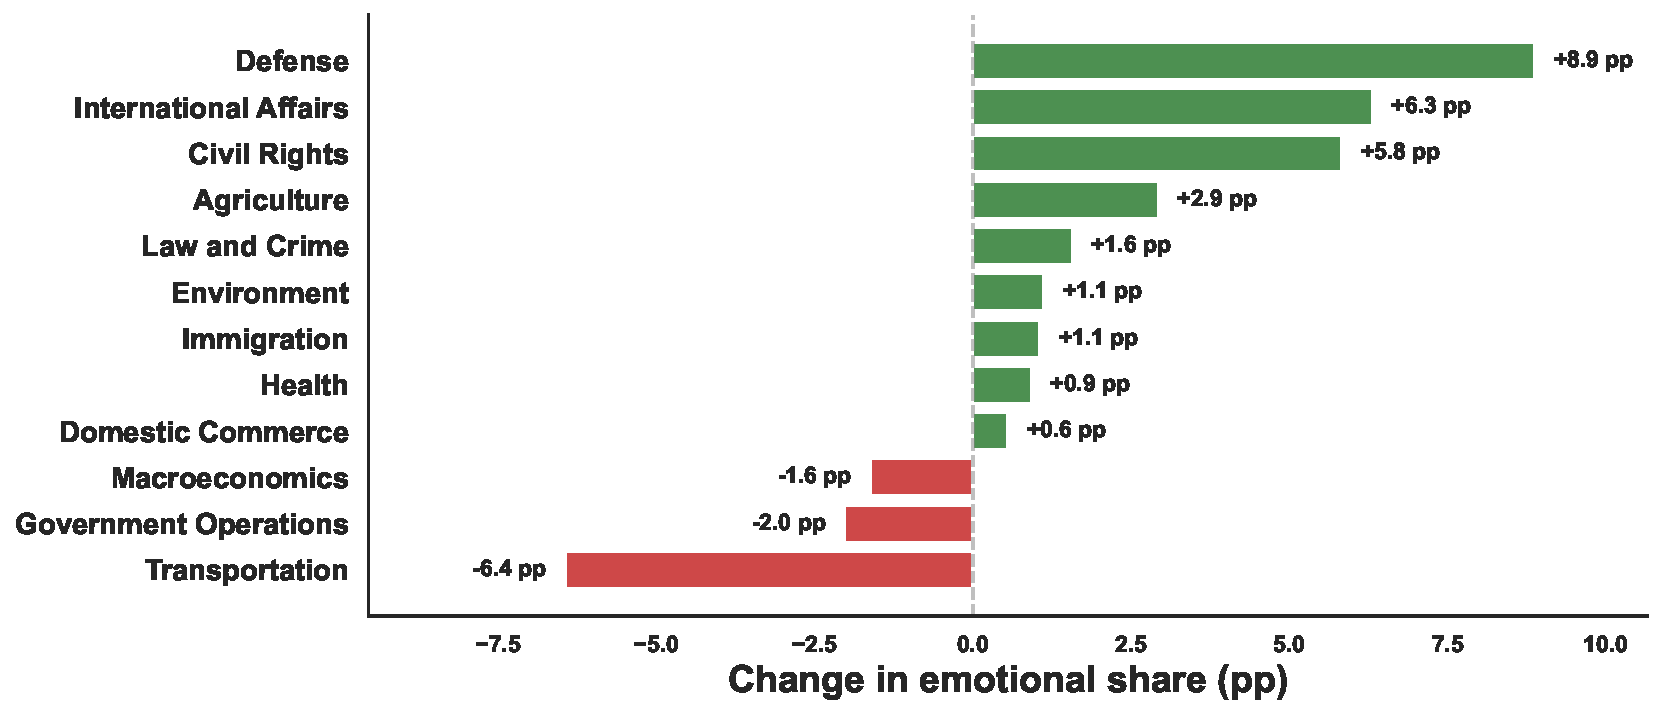
\includegraphics[width=0.80\textwidth,height=0.76\textheight,keepaspectratio]{staenderat_fig_lt_defD_topic_shift.pdf}
    \vfill
    {\footnotesize\hyperlink{main.SR.emotion}{Back to condensed Ständerat slide}.}
    \end{frame}
\begin{frame}{Appendix --- Emotional Rhetoric by Topic and Party --- Ständerat}
    \centering
    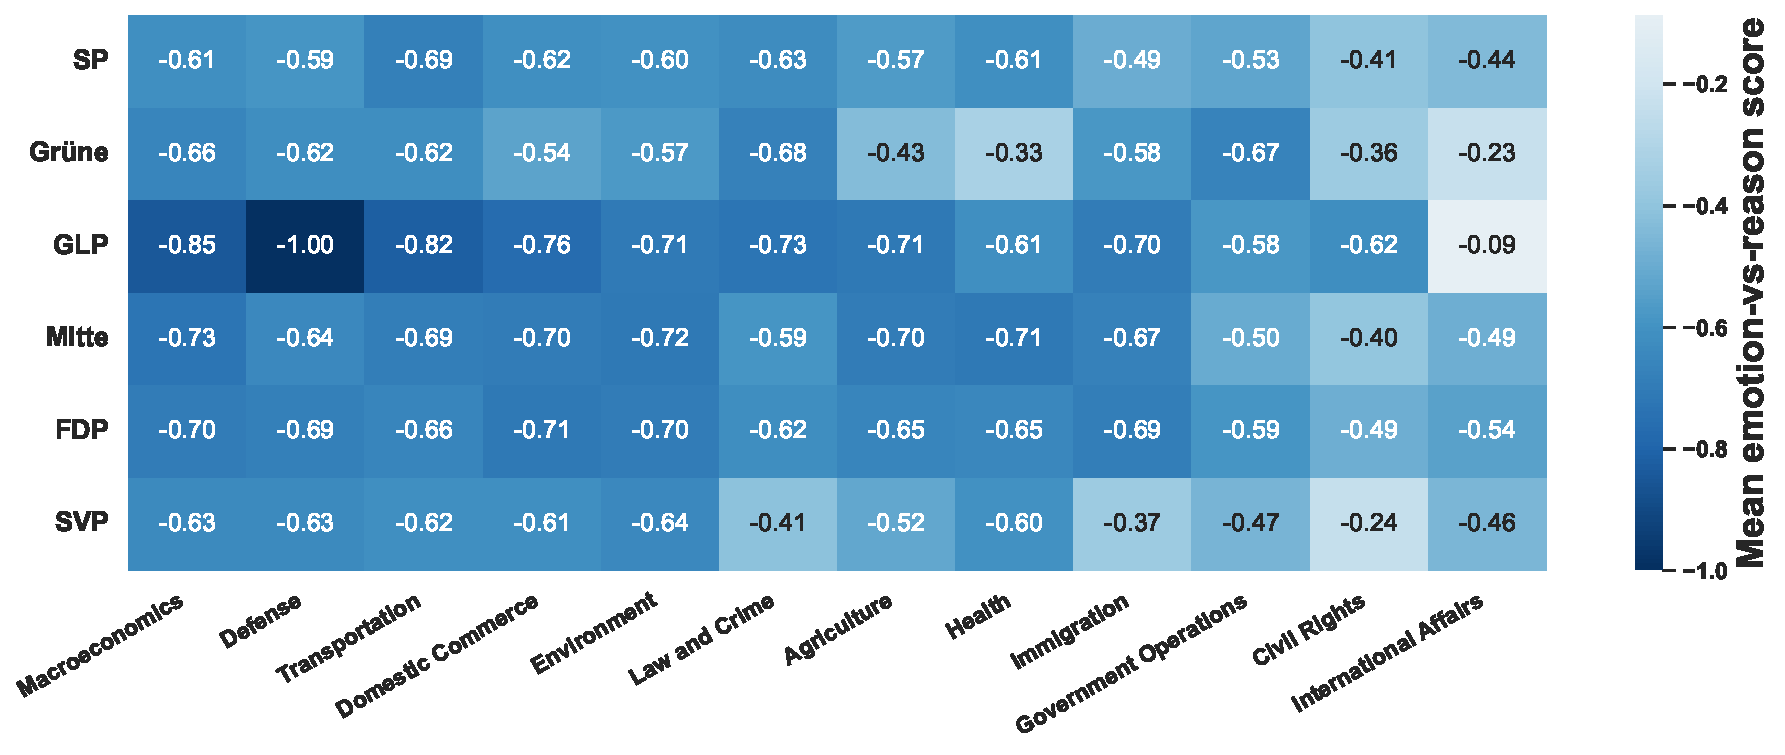
\includegraphics[width=0.78\textwidth,height=0.76\textheight,keepaspectratio]{staenderat_fig_lt_emotionality_topic_by_party_heatmap.pdf}
    \vfill
    {\footnotesize\hyperlink{main.SR.emotion}{Back to condensed Ständerat slide}.}
    \end{frame}
\begin{frame}{Appendix --- Emotional Rhetoric by Topic, One Panel per Party --- Ständerat}
    \centering
    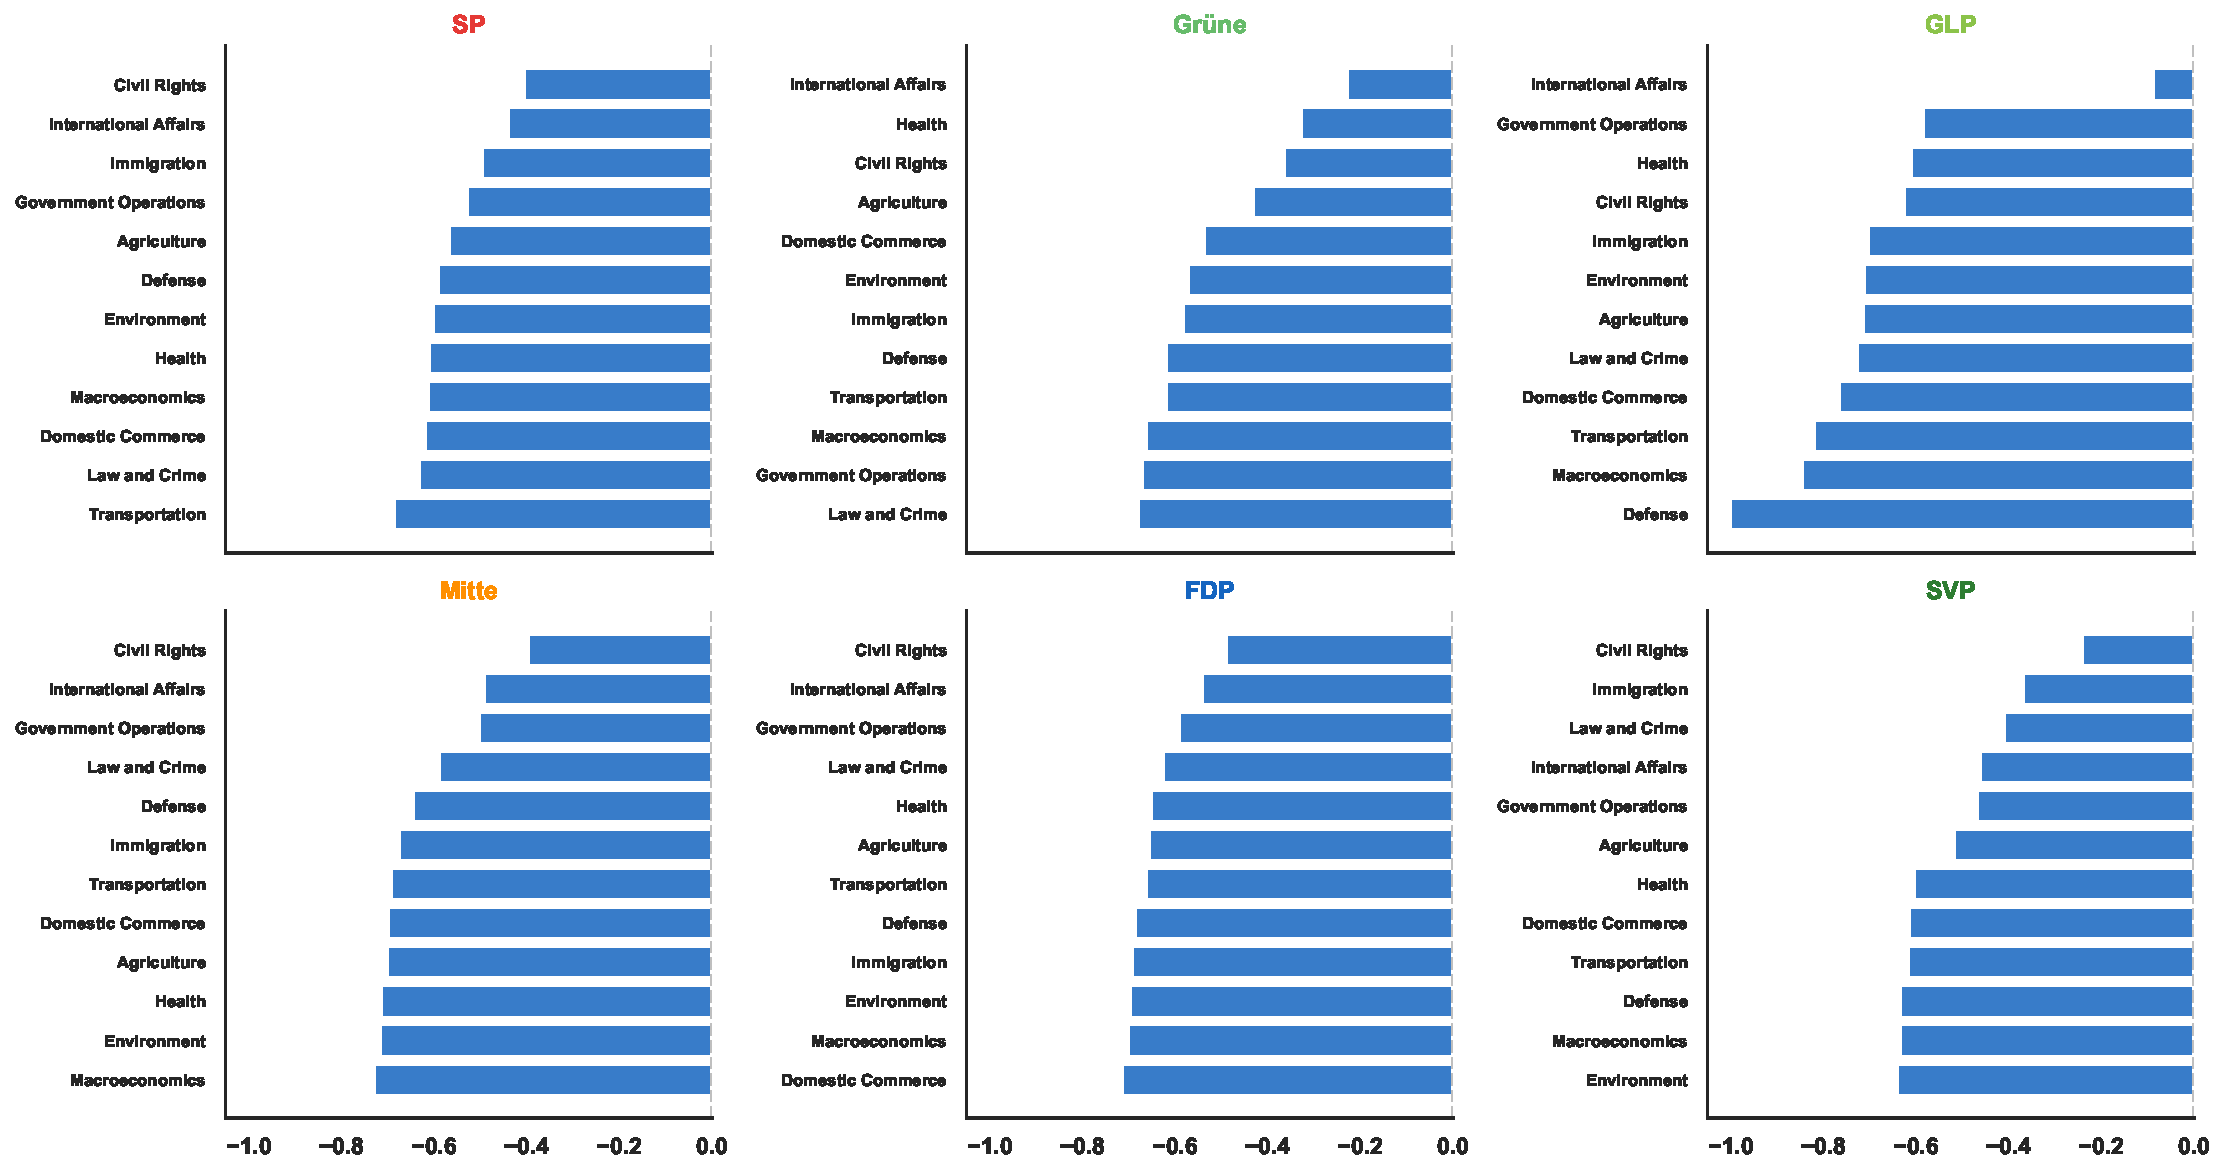
\includegraphics[width=0.86\textwidth,height=0.76\textheight,keepaspectratio]{staenderat_fig_lt_emotionality_topic_by_party_bars.pdf}
    \vfill
    {\footnotesize\hyperlink{main.SR.emotion}{Back to condensed Ständerat slide}.}
    \end{frame}
\begin{frame}{Appendix --- Who Drives Emotional-Rhetoric Shifts Within Topics? --- Ständerat}
    \centering
    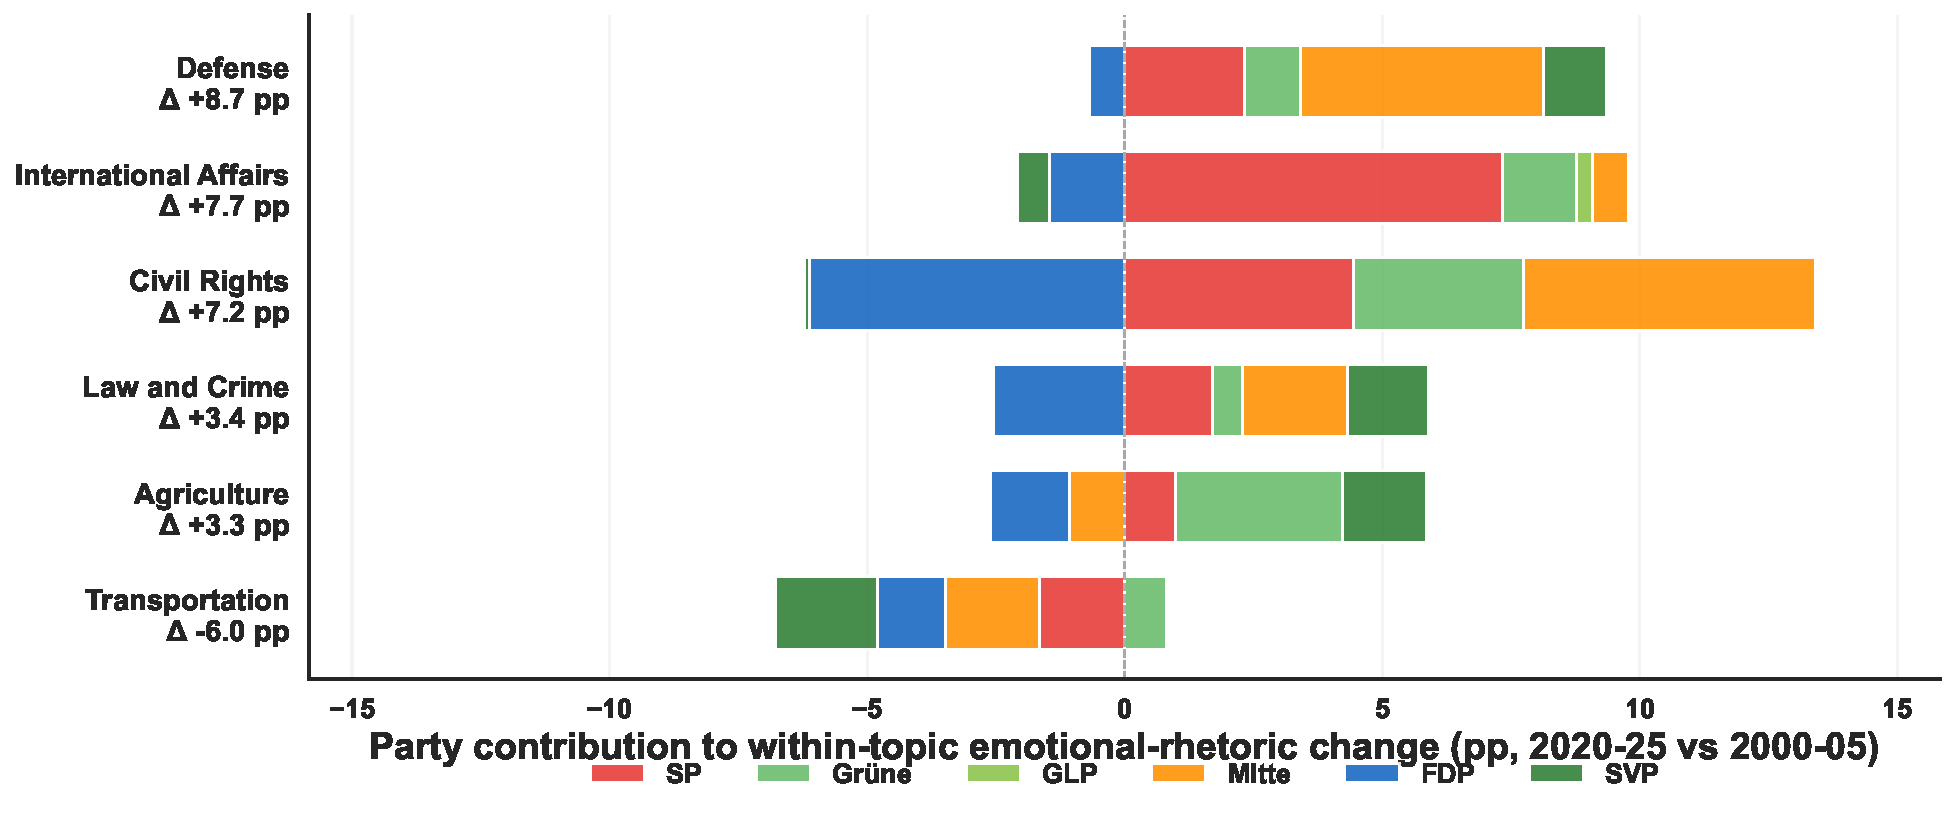
\includegraphics[width=0.88\textwidth,height=0.76\textheight,keepaspectratio]{staenderat_fig_emotion_shift_within_topic_drivers_by_party.pdf}
    \vfill
    {\footnotesize\hyperlink{main.SR.emotion}{Back to condensed Ständerat slide}.}
    \end{frame}
\begin{frame}{Appendix --- Emotional-Rhetoric Shift Contributions by Party --- Ständerat}
    \centering
    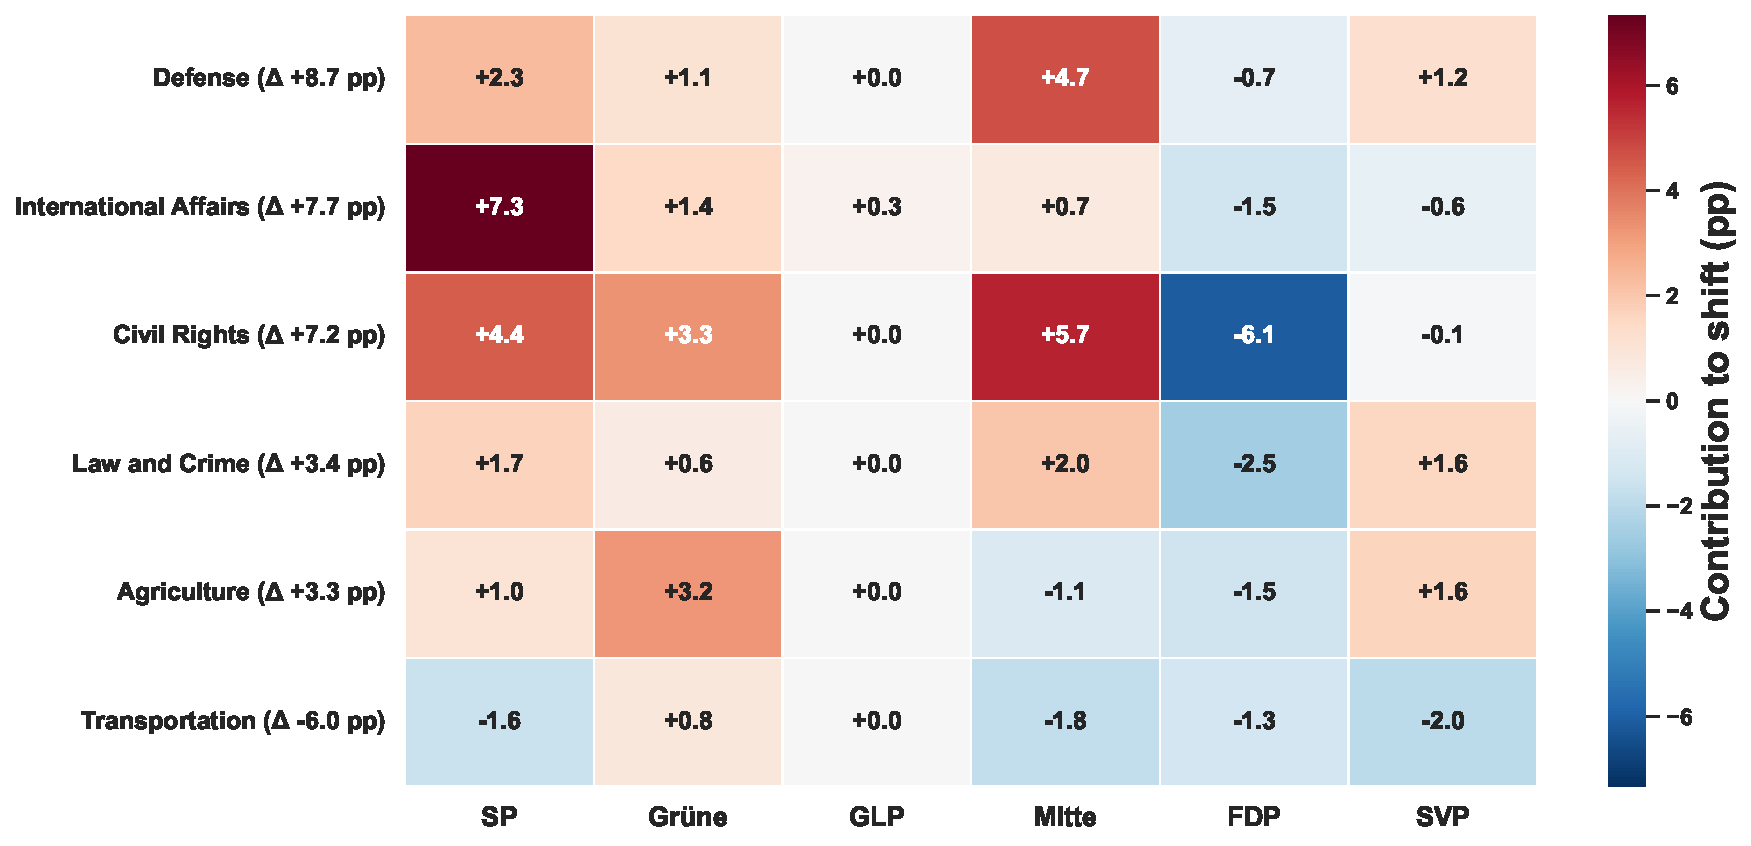
\includegraphics[width=0.88\textwidth,height=0.76\textheight,keepaspectratio]{staenderat_fig_emotion_shift_within_topic_driver_table.pdf}
    \vfill
    {\footnotesize\hyperlink{main.SR.emotion}{Back to condensed Ständerat slide}.}
    \end{frame}
\begin{frame}{Appendix --- Emotional Rhetoric by Topic --- 2000--05 vs 2020--24 --- Ständerat}
\centering
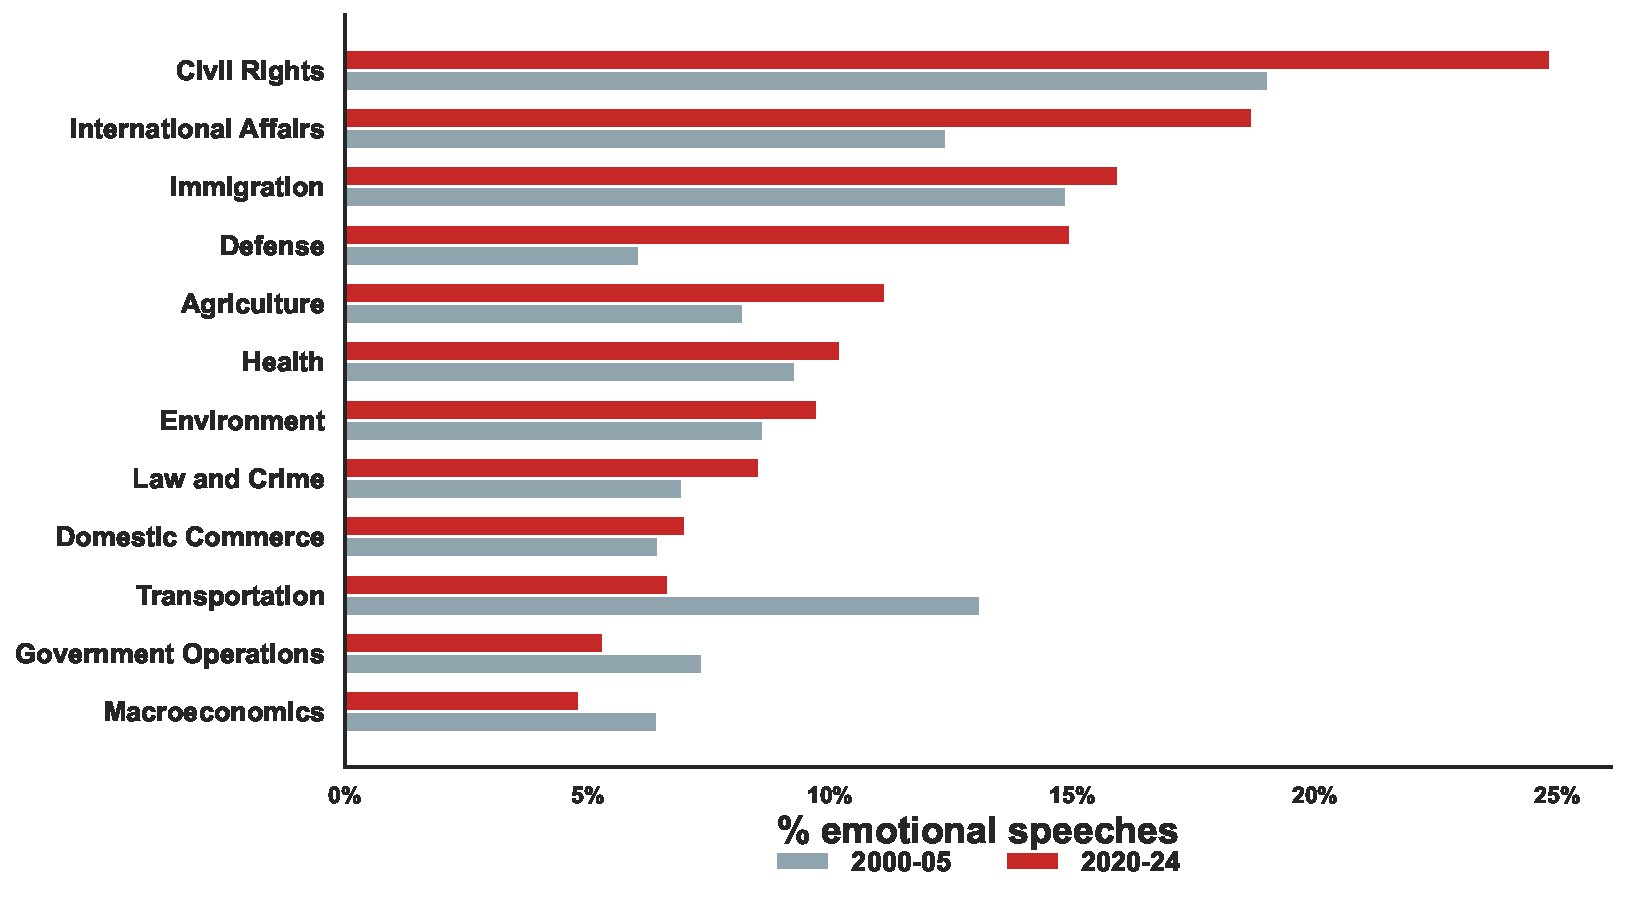
\includegraphics[width=0.86\textwidth,height=0.70\textheight,keepaspectratio]{staenderat_fig_lt_defD_by_topic.pdf}
\vfill
{\footnotesize\textit{Note:} Bars pool all six parties; GLP had minimal Council of States floor time in 2000--05. \hyperlink{main.SR.emotion}{Back}.}
\end{frame}

\begin{frame}{Appendix --- Gender Representation by Party --- Ständerat}
\hypertarget{app.SR.gender}{}
\centering
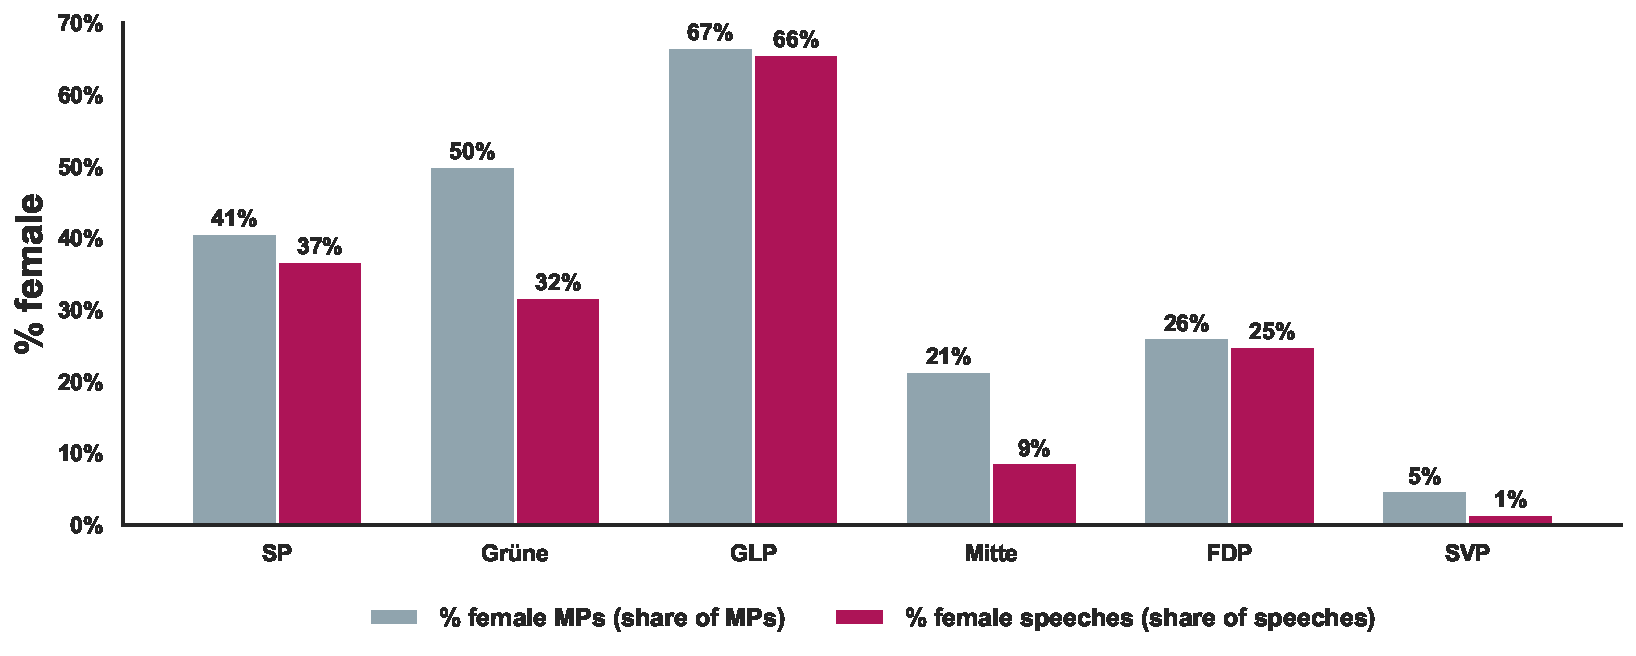
\includegraphics[width=0.82\textwidth,height=0.76\textheight,keepaspectratio]{staenderat_fig_lt_gender_mp_vs_speeches_party.pdf}
\vfill
{\footnotesize\hyperlink{main.SR.gender}{Back to condensed Ständerat gender slide}.}
\end{frame}
\begin{frame}{Appendix --- Canton Share of Speeches --- Ständerat}
    \centering
    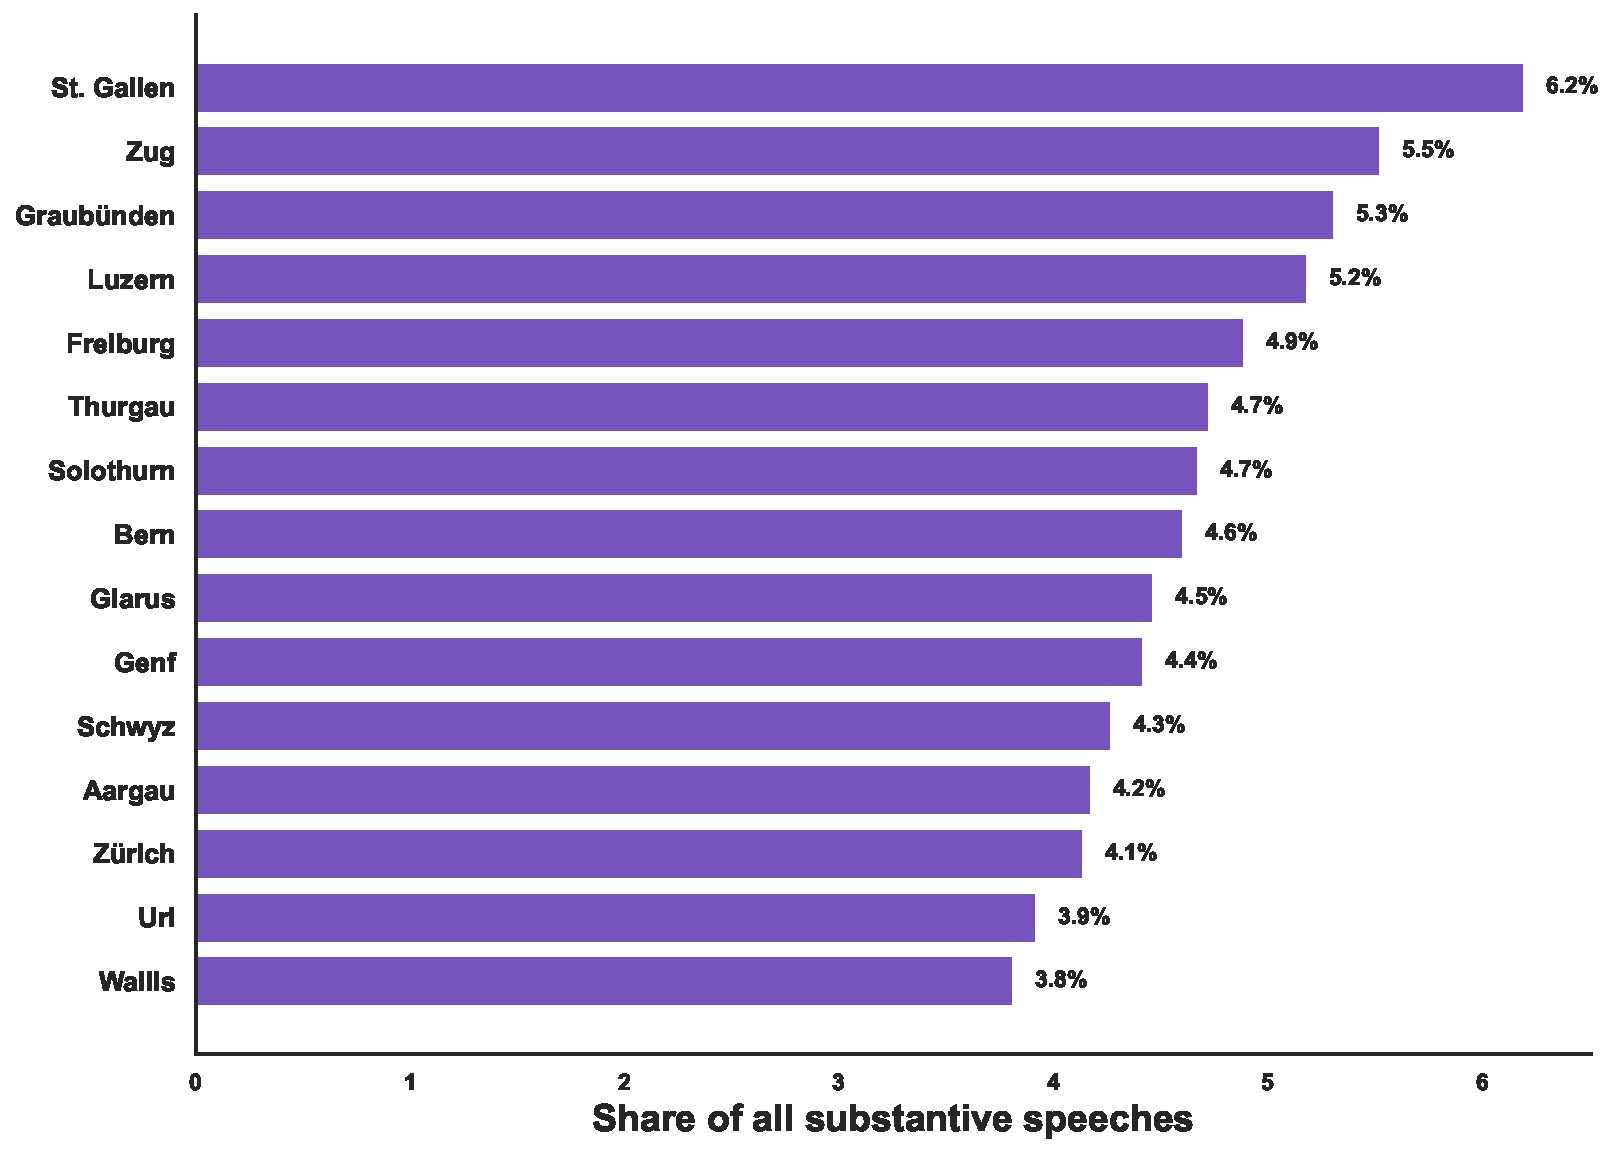
\includegraphics[width=0.70\textwidth,height=0.76\textheight,keepaspectratio]{staenderat_fig_lt_canton_share.pdf}
    \vfill
    {\footnotesize\hyperlink{main.SR.gender}{Back to condensed Ständerat slide}.}
    \end{frame}
\begin{frame}{Appendix --- Canton Speeches per MP --- Ständerat}
    \centering
    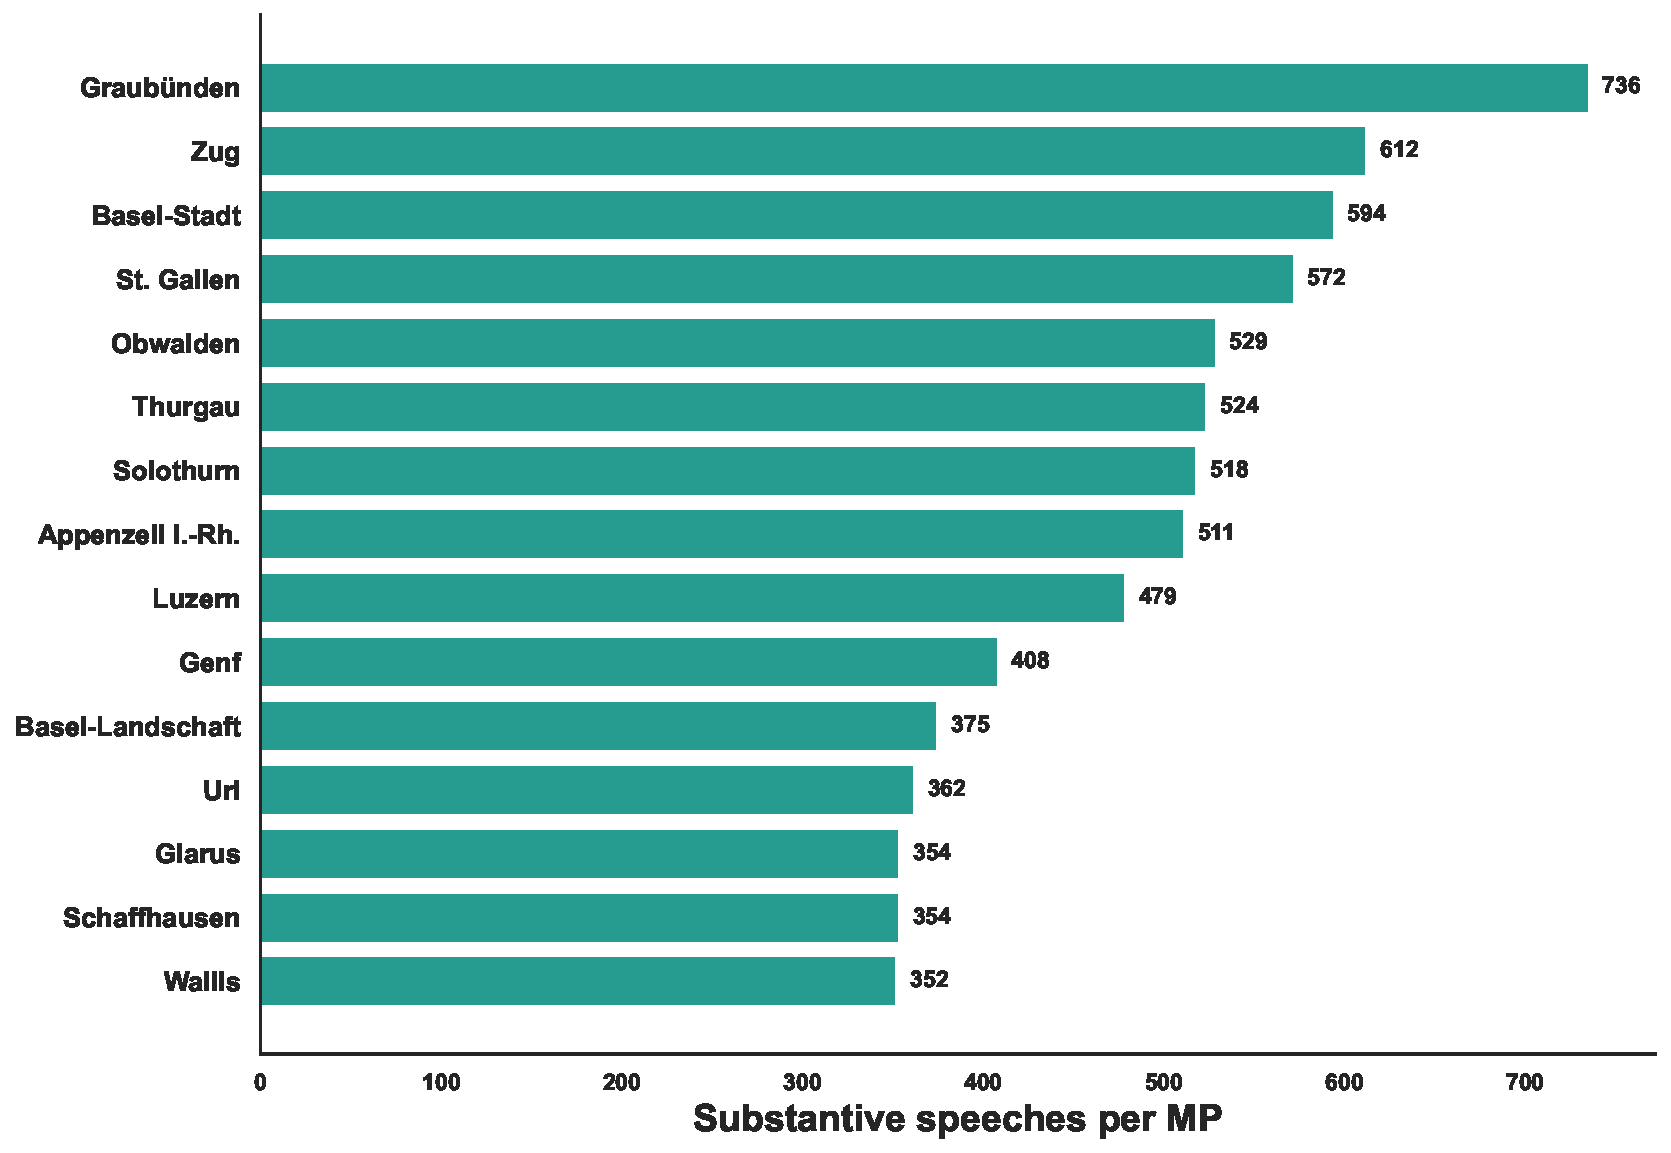
\includegraphics[width=0.78\textwidth,height=0.76\textheight,keepaspectratio]{staenderat_fig_lt_canton_per_mp.pdf}
    \vfill
    {\footnotesize\hyperlink{main.SR.gender}{Back to condensed Ständerat slide}.}
    \end{frame}
\begin{frame}{Appendix --- Floor-Time Gap by Canton --- Ständerat}
    \centering
    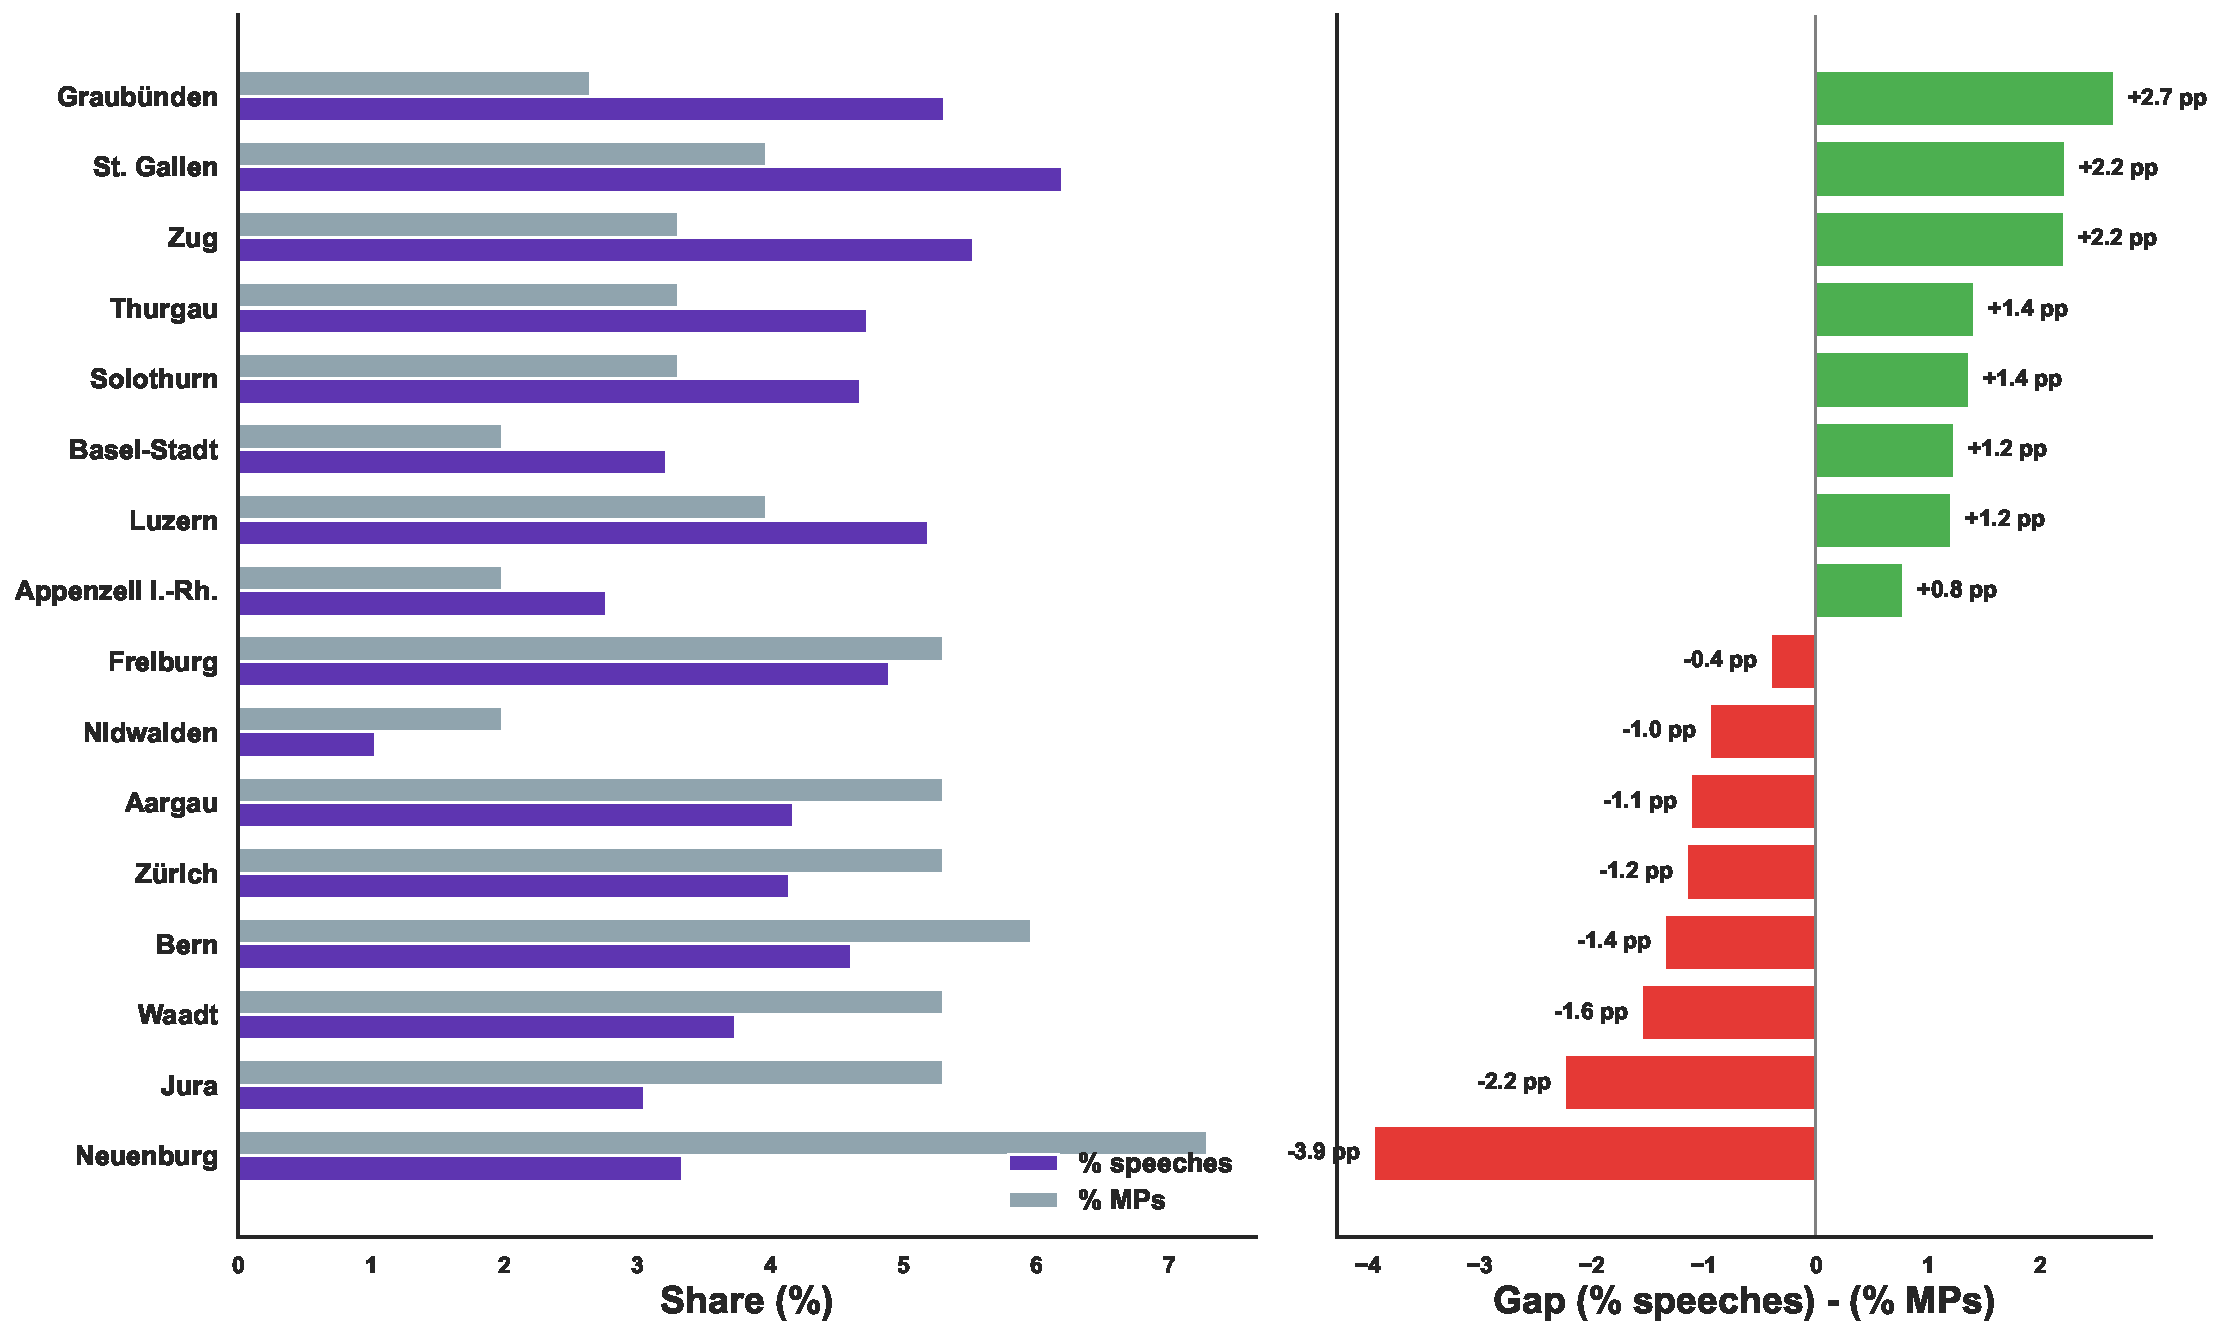
\includegraphics[width=0.88\textwidth,height=0.76\textheight,keepaspectratio]{staenderat_fig_lt_canton_gap.pdf}
    \vfill
    {\footnotesize\hyperlink{main.SR.gender}{Back to condensed Ständerat slide}.}
    \end{frame}
\begin{frame}{Appendix --- Emotional Rhetoric by Generation of MPs --- Ständerat}
\centering
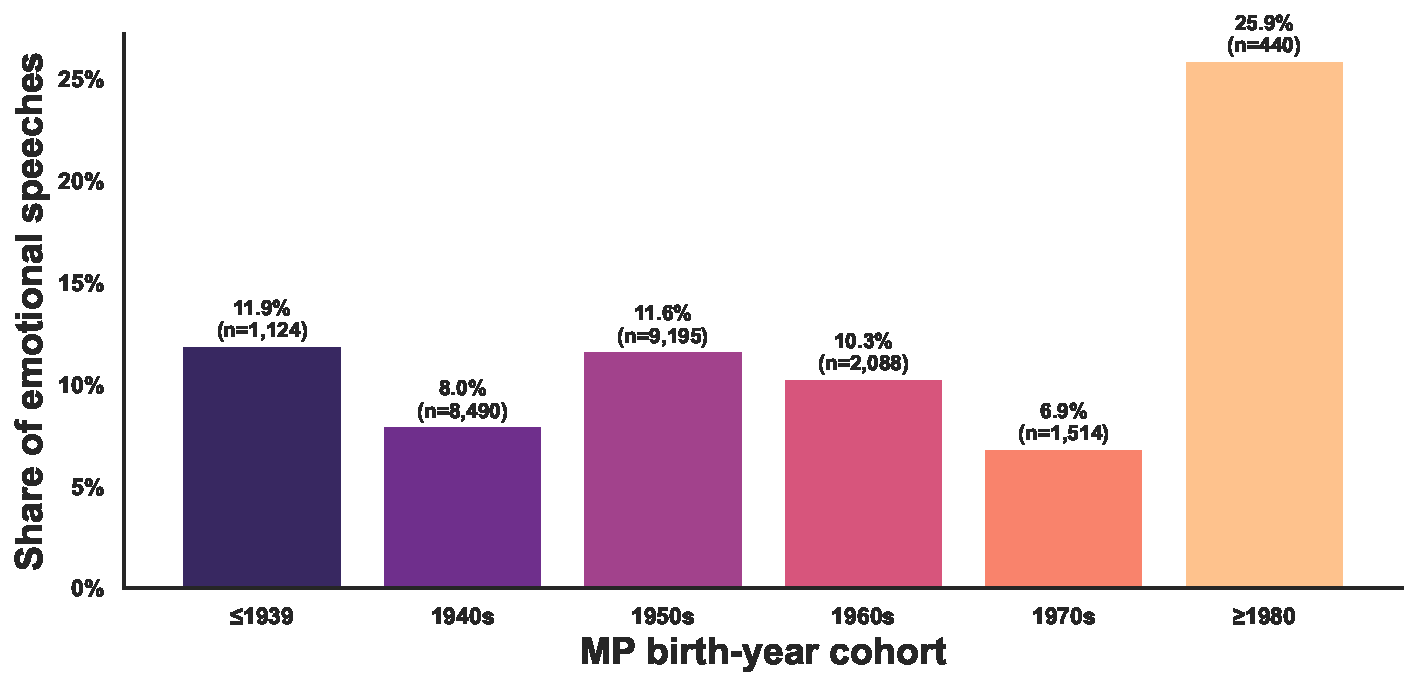
\includegraphics[width=0.82\textwidth,height=0.74\textheight,keepaspectratio]{staenderat_fig_lt_cohort_emotional.pdf}
\vfill
{\footnotesize\textit{Note:} Younger birth cohorts appear here mostly at ages under~50; older cohorts mostly over~50 in this corpus window. Level differences can mix a \textbf{cohort} story with an \textbf{age-at-speech} story. \hyperlink{main.SR.gender}{Back to condensed Ständerat gender slide}.}
\end{frame}
\begin{frame}{Appendix --- Emotional Rhetoric by Age Group --- Ständerat}
    \centering
    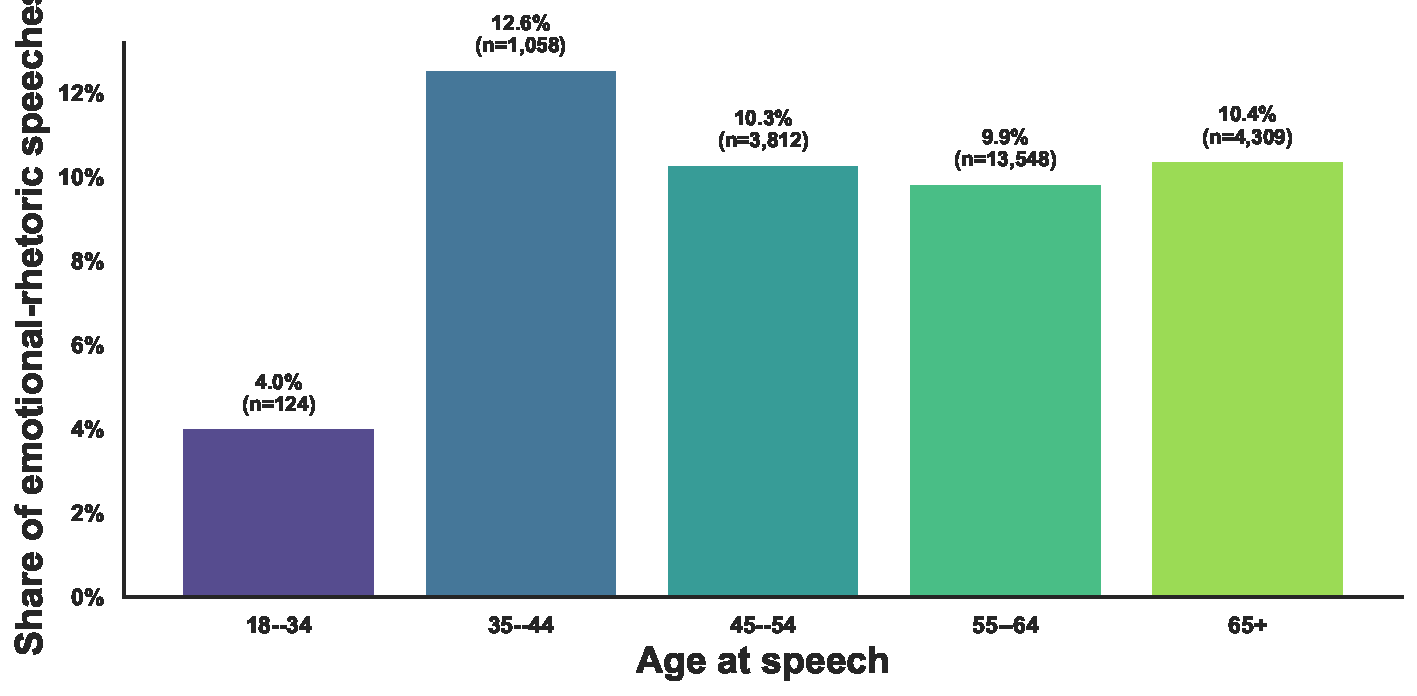
\includegraphics[width=0.82\textwidth,height=0.76\textheight,keepaspectratio]{staenderat_fig_lt_age_group_emotional.pdf}
    \vfill
    {\footnotesize\hyperlink{main.SR.gender}{Back to condensed Ständerat slide}.}
    \end{frame}
\begin{frame}{Appendix --- Emotional Rhetoric by Language of the Speech --- Ständerat}
    \centering
    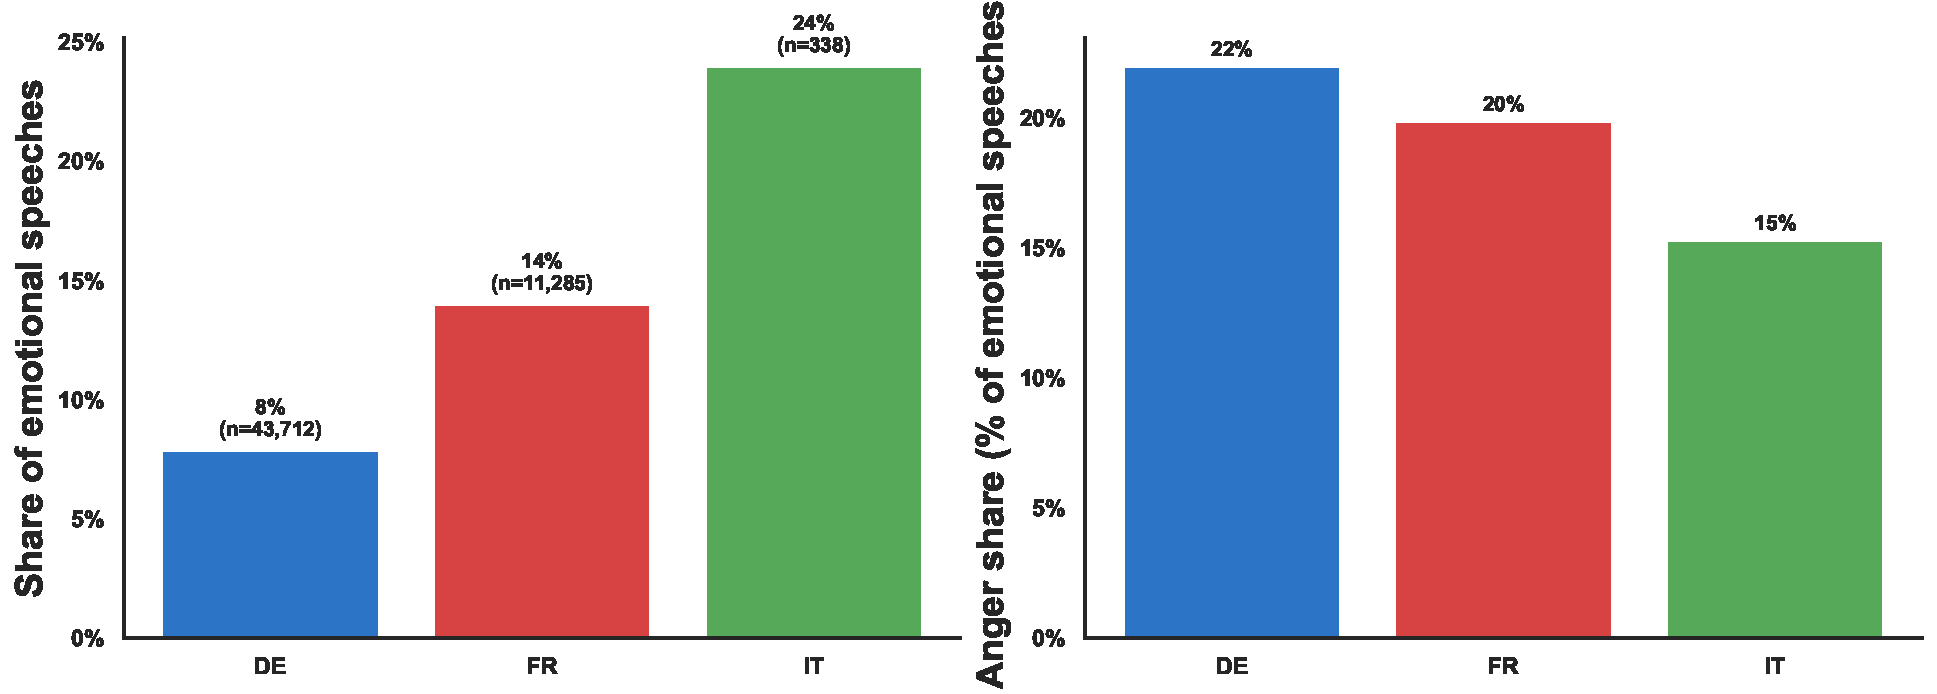
\includegraphics[width=0.95\textwidth,height=0.76\textheight,keepaspectratio]{staenderat_fig_lt_emotion_language.pdf}
    \vfill
    {\footnotesize\hyperlink{main.SR.gender}{Back to condensed Ständerat slide}.}
    \end{frame}
\begin{frame}{Appendix --- Applause by Party --- Ständerat}
\begin{columns}[T]
\begin{column}{0.49\textwidth}
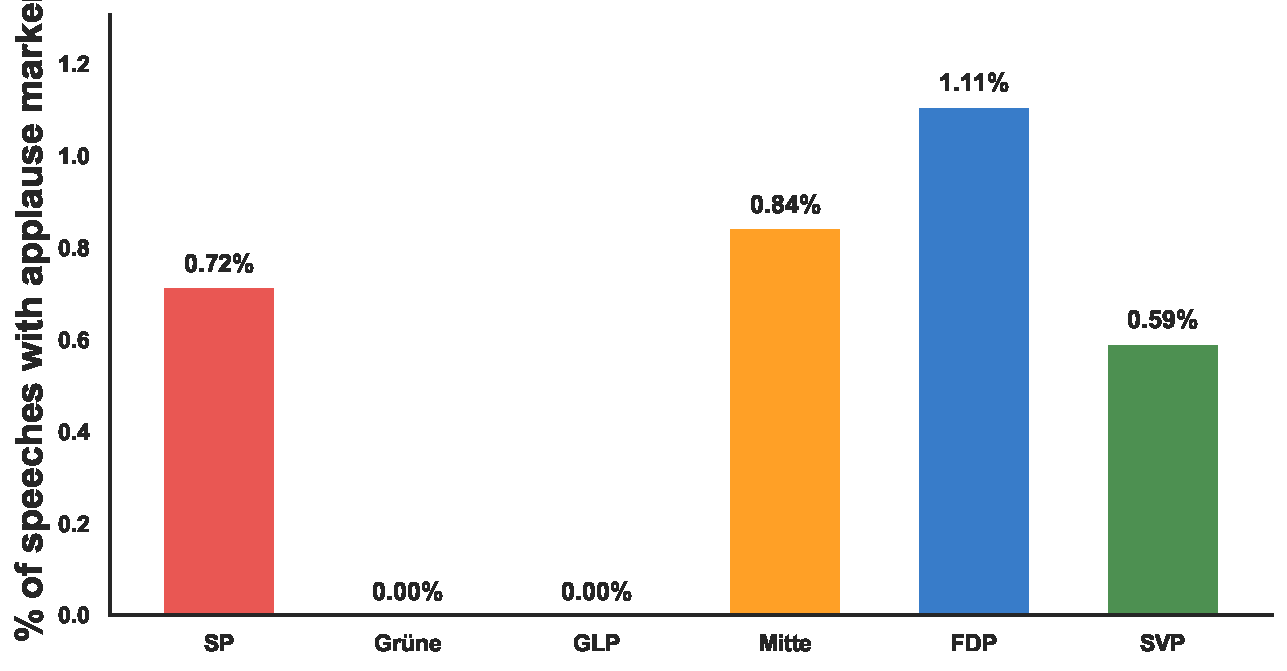
\includegraphics[width=\textwidth]{staenderat_fig_app_rate_by_party.pdf}
\end{column}
\begin{column}{0.49\textwidth}
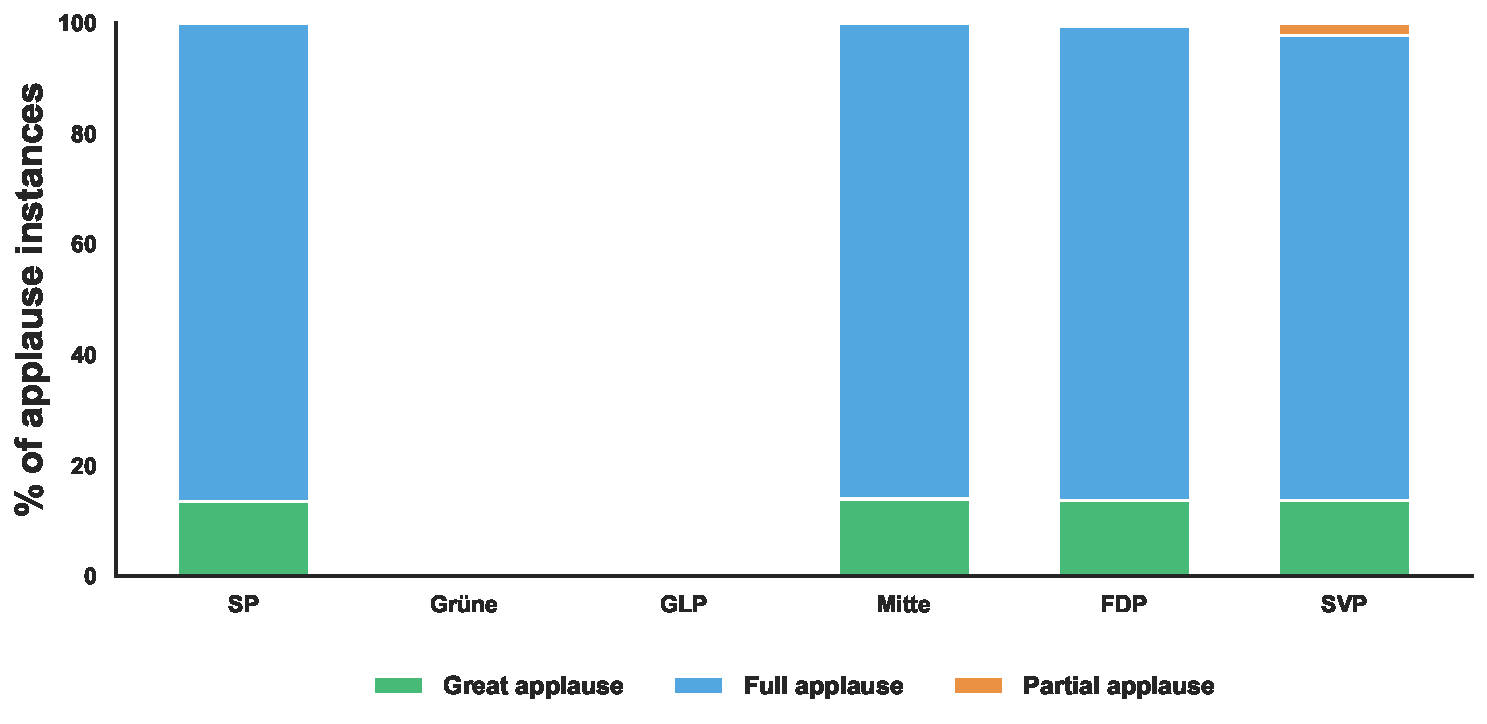
\includegraphics[width=\textwidth]{staenderat_fig_app_type_by_party.pdf}
\end{column}
\end{columns}
\vfill
{\footnotesize\hyperlink{main.SR.gender}{Back to condensed Ständerat gender slide}.}
\end{frame}
\begin{frame}{Appendix --- Most Applauded Parliamentarians --- Ständerat}
    \centering
    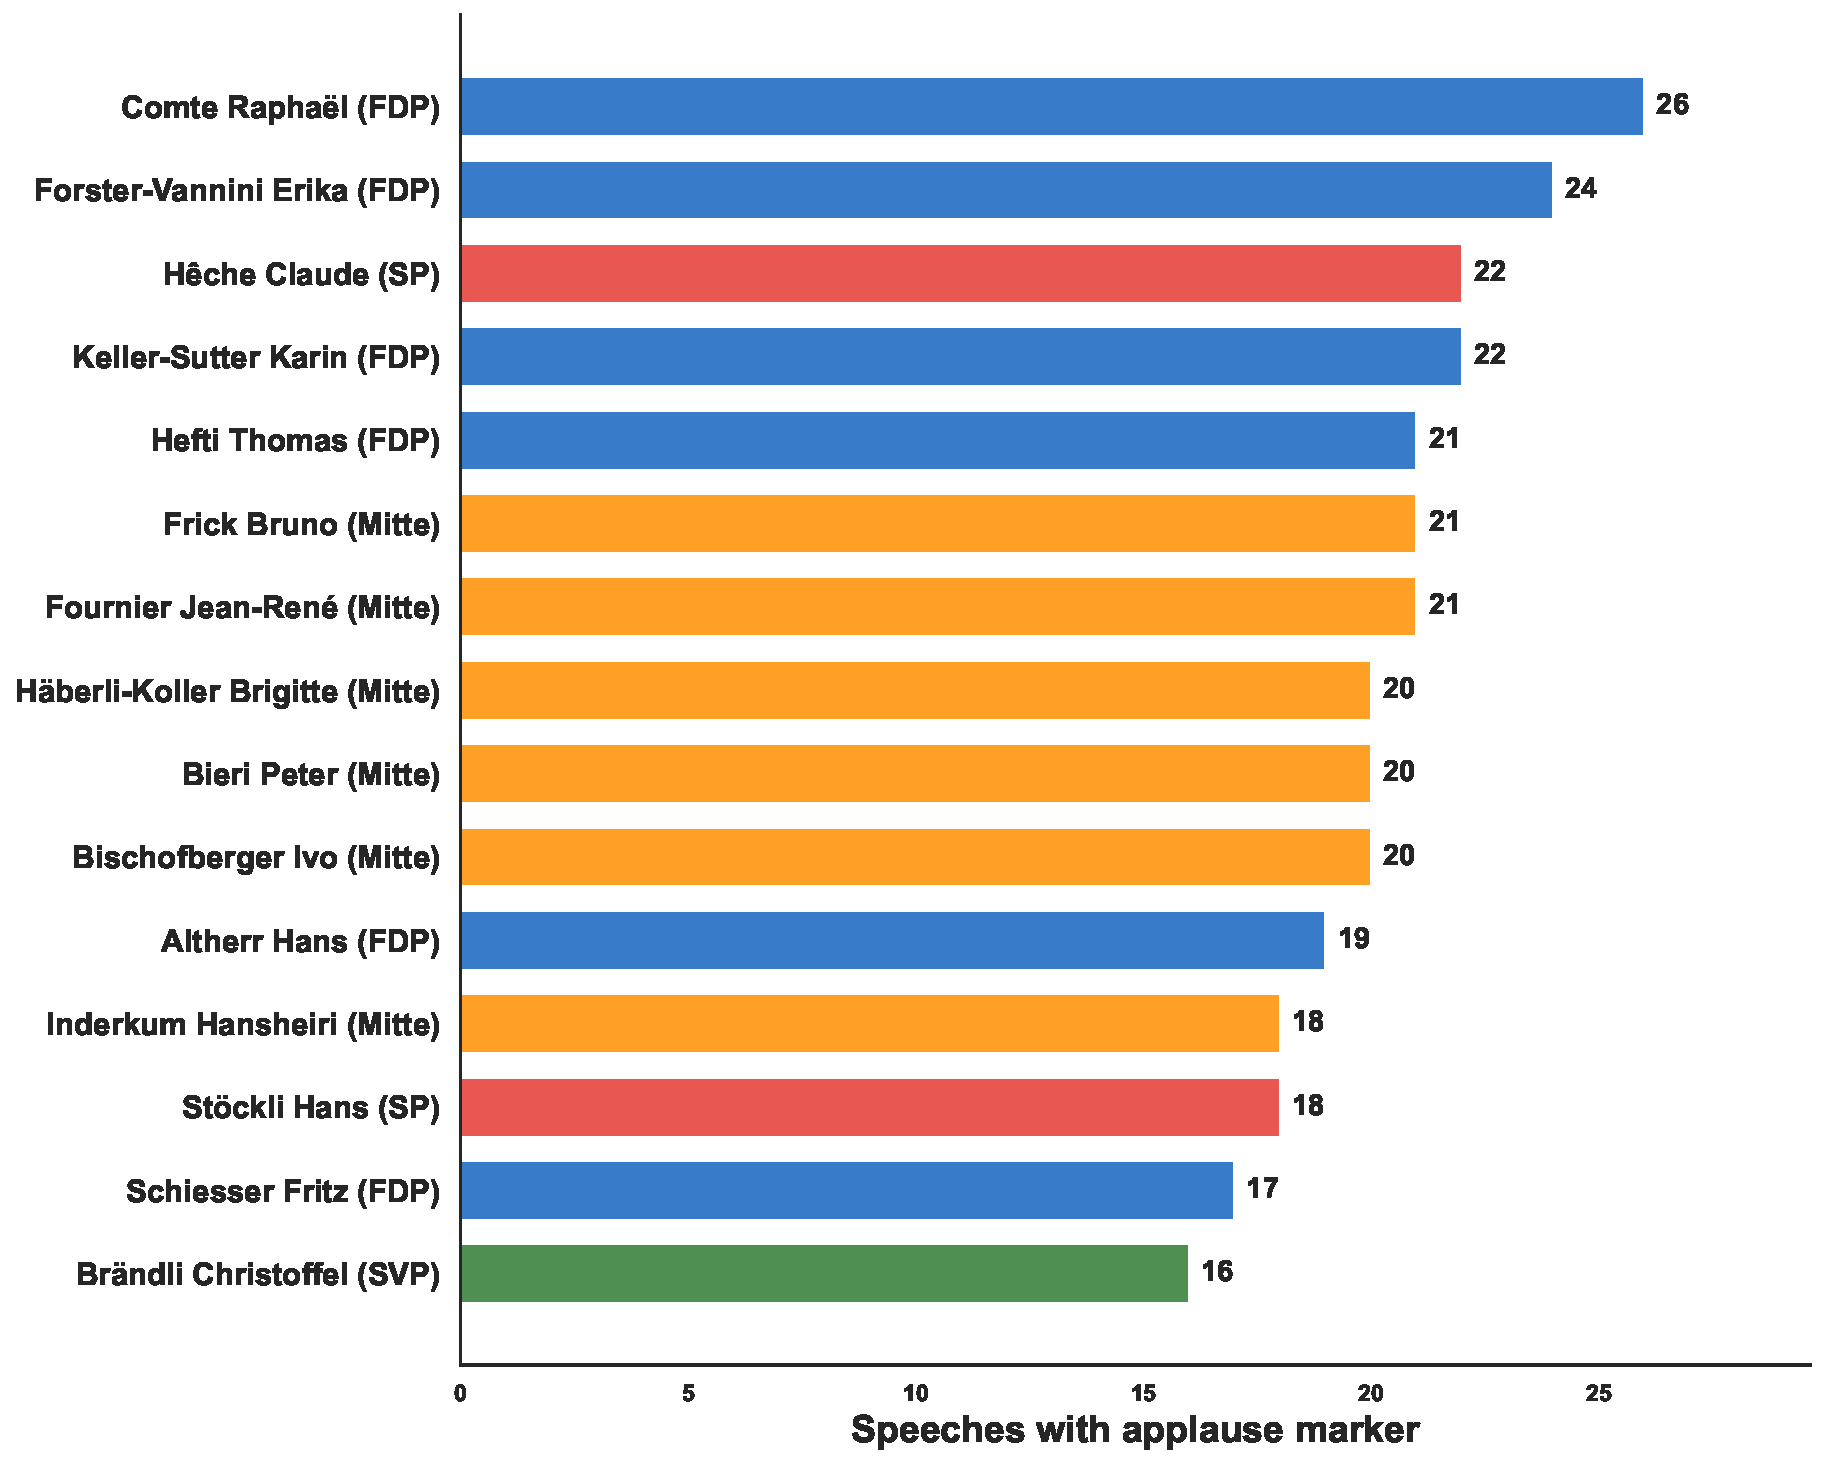
\includegraphics[width=0.96\textwidth,height=0.76\textheight,keepaspectratio]{staenderat_fig_app_top_mps.pdf}
    \vfill
    {\footnotesize\hyperlink{main.SR.gender}{Back to condensed Ständerat slide}.}
    \end{frame}

\begin{frame}{Appendix --- Emotional-Rhetoric Shift Contributions by Party --- Nationalrat}
\hypertarget{app.NR.emotion.drivers.table}{}
\centering
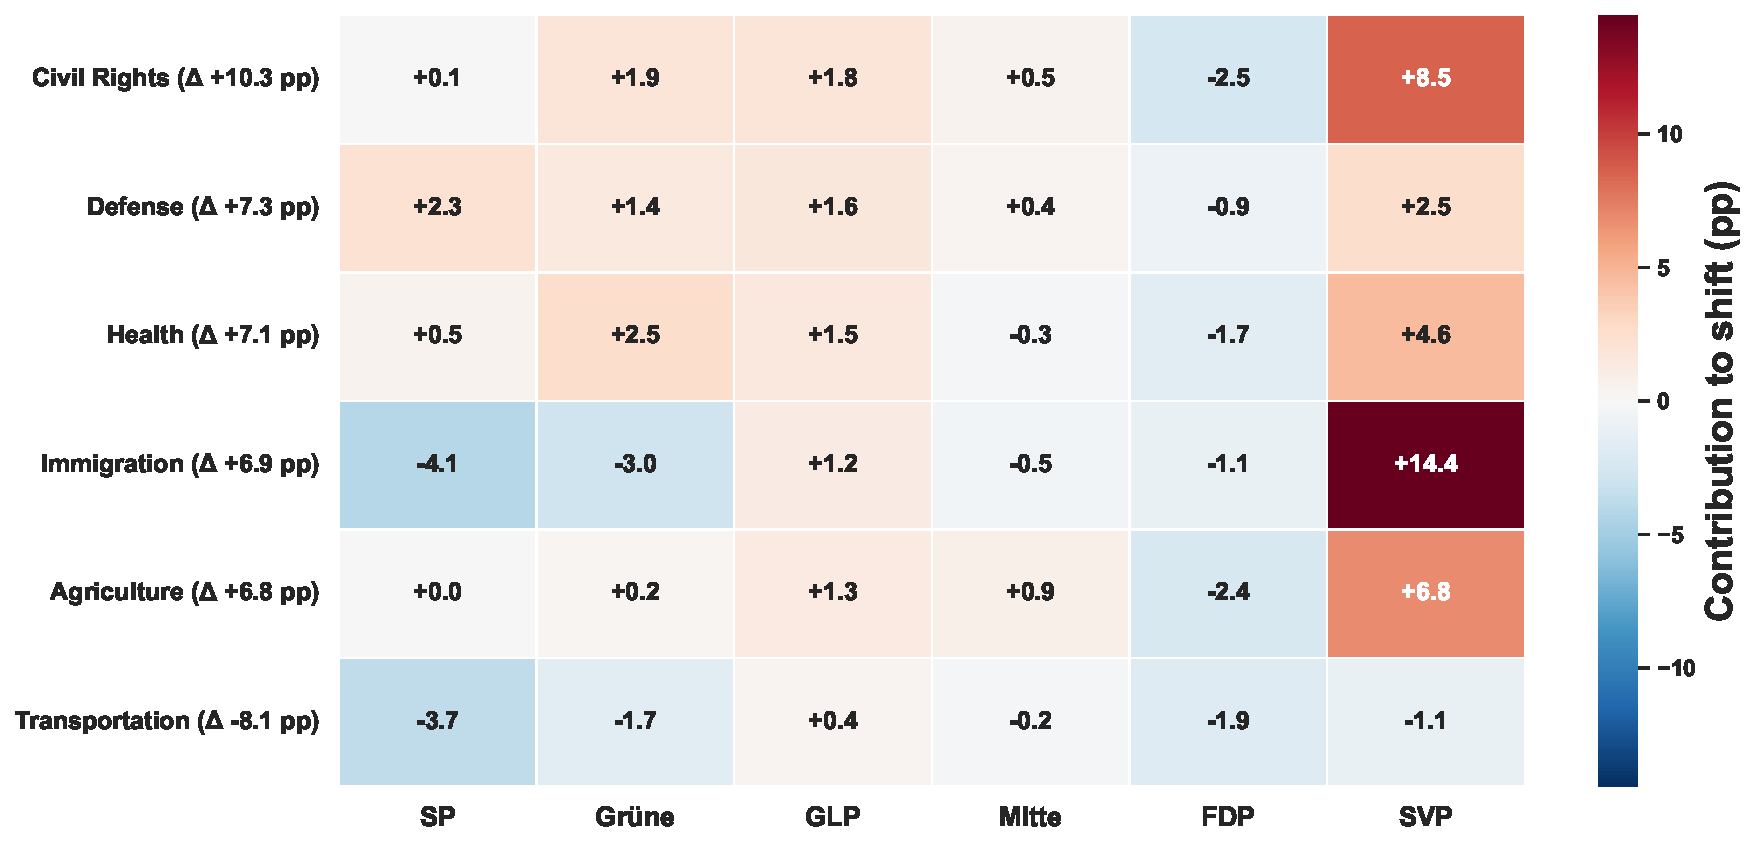
\includegraphics[width=0.88\textwidth,height=0.76\textheight,keepaspectratio]{nationalrat_fig_emotion_shift_within_topic_driver_table.pdf}
\vfill
{\footnotesize\hyperlink{main.NR.emotion.drivers}{Back to main emotion-shift driver figure}.}
\end{frame}
\begin{frame}{Appendix --- Emotional Rhetoric by Topic and Party --- Nationalrat}
    \centering
    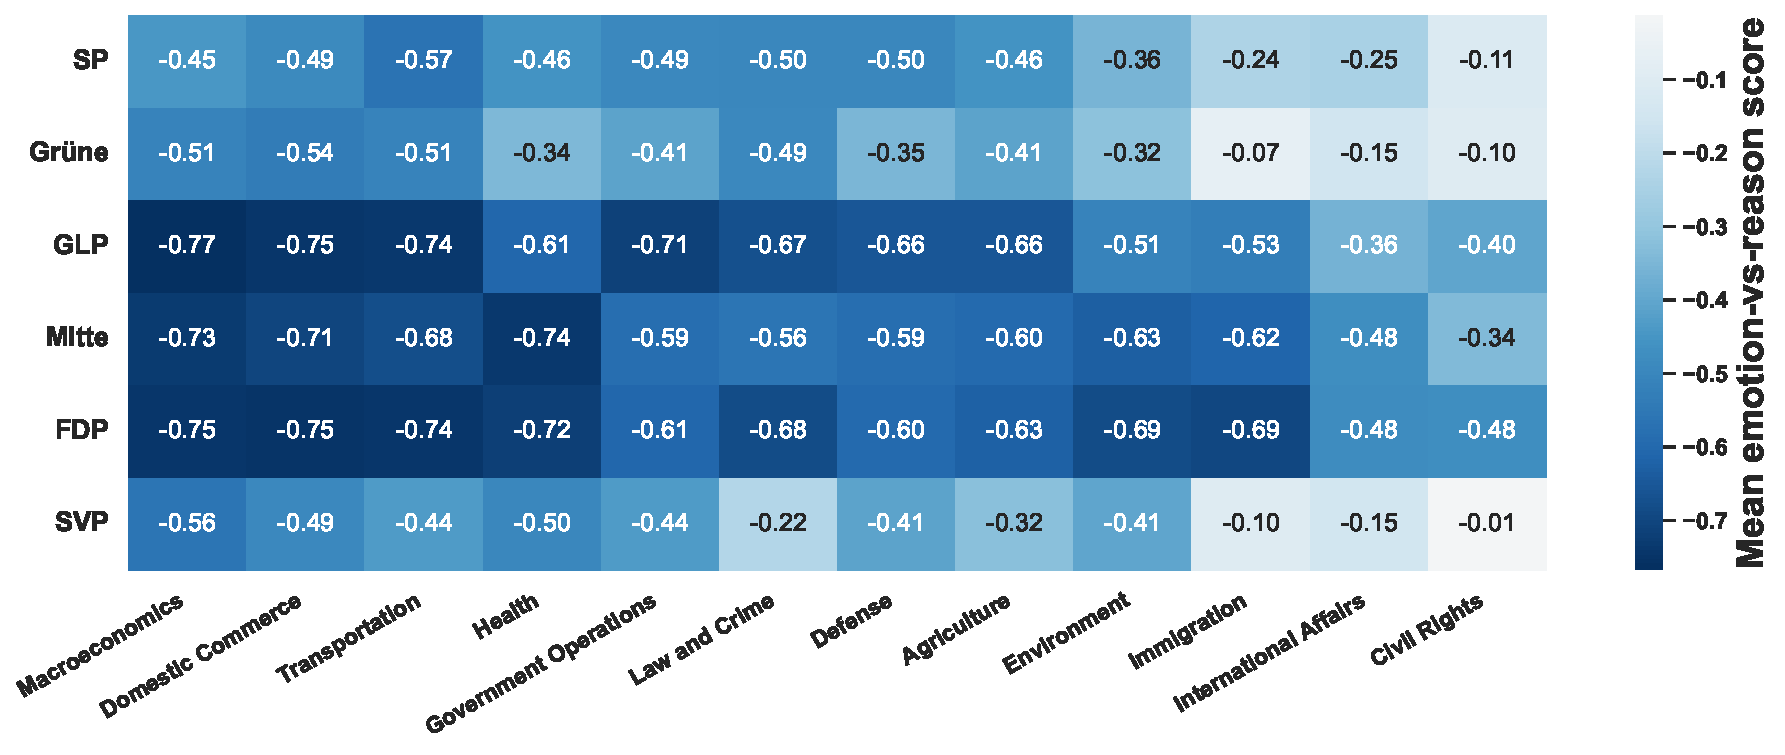
\includegraphics[width=0.78\textwidth,height=0.82\textheight,keepaspectratio]{fig_lt_emotionality_topic_by_party_heatmap.pdf}
    \end{frame}
\begin{frame}{Appendix --- Emotional Rhetoric by Topic, One Panel per Party --- Nationalrat}
    \centering
    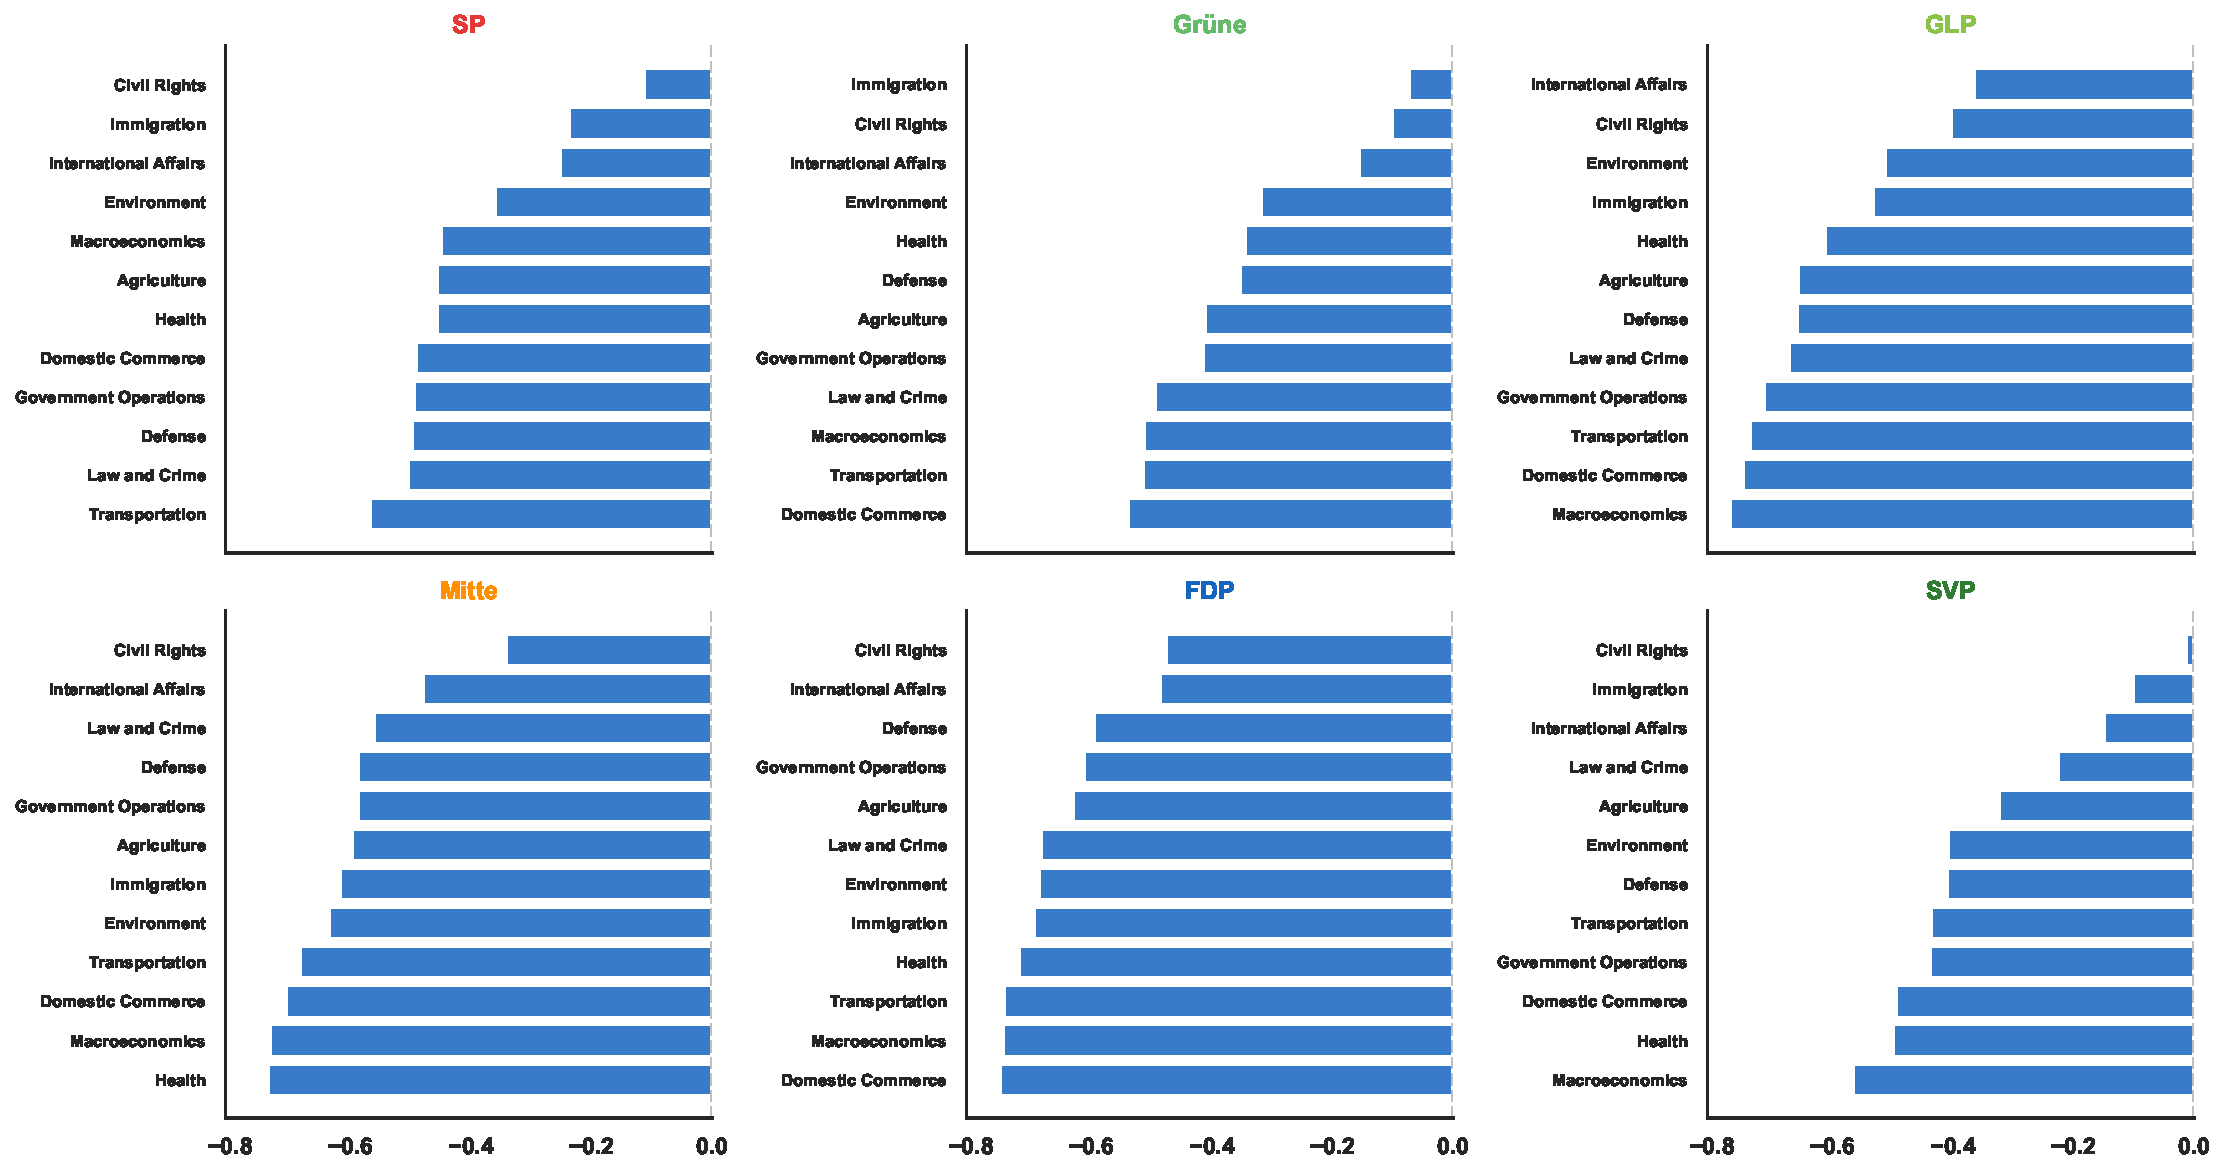
\includegraphics[width=0.86\textwidth,height=0.82\textheight,keepaspectratio]{fig_lt_emotionality_topic_by_party_bars.pdf}
    \end{frame}
\begin{frame}{Appendix --- Emotional-Rhetoric Shift by Topic and Party --- Nationalrat}
    \centering
    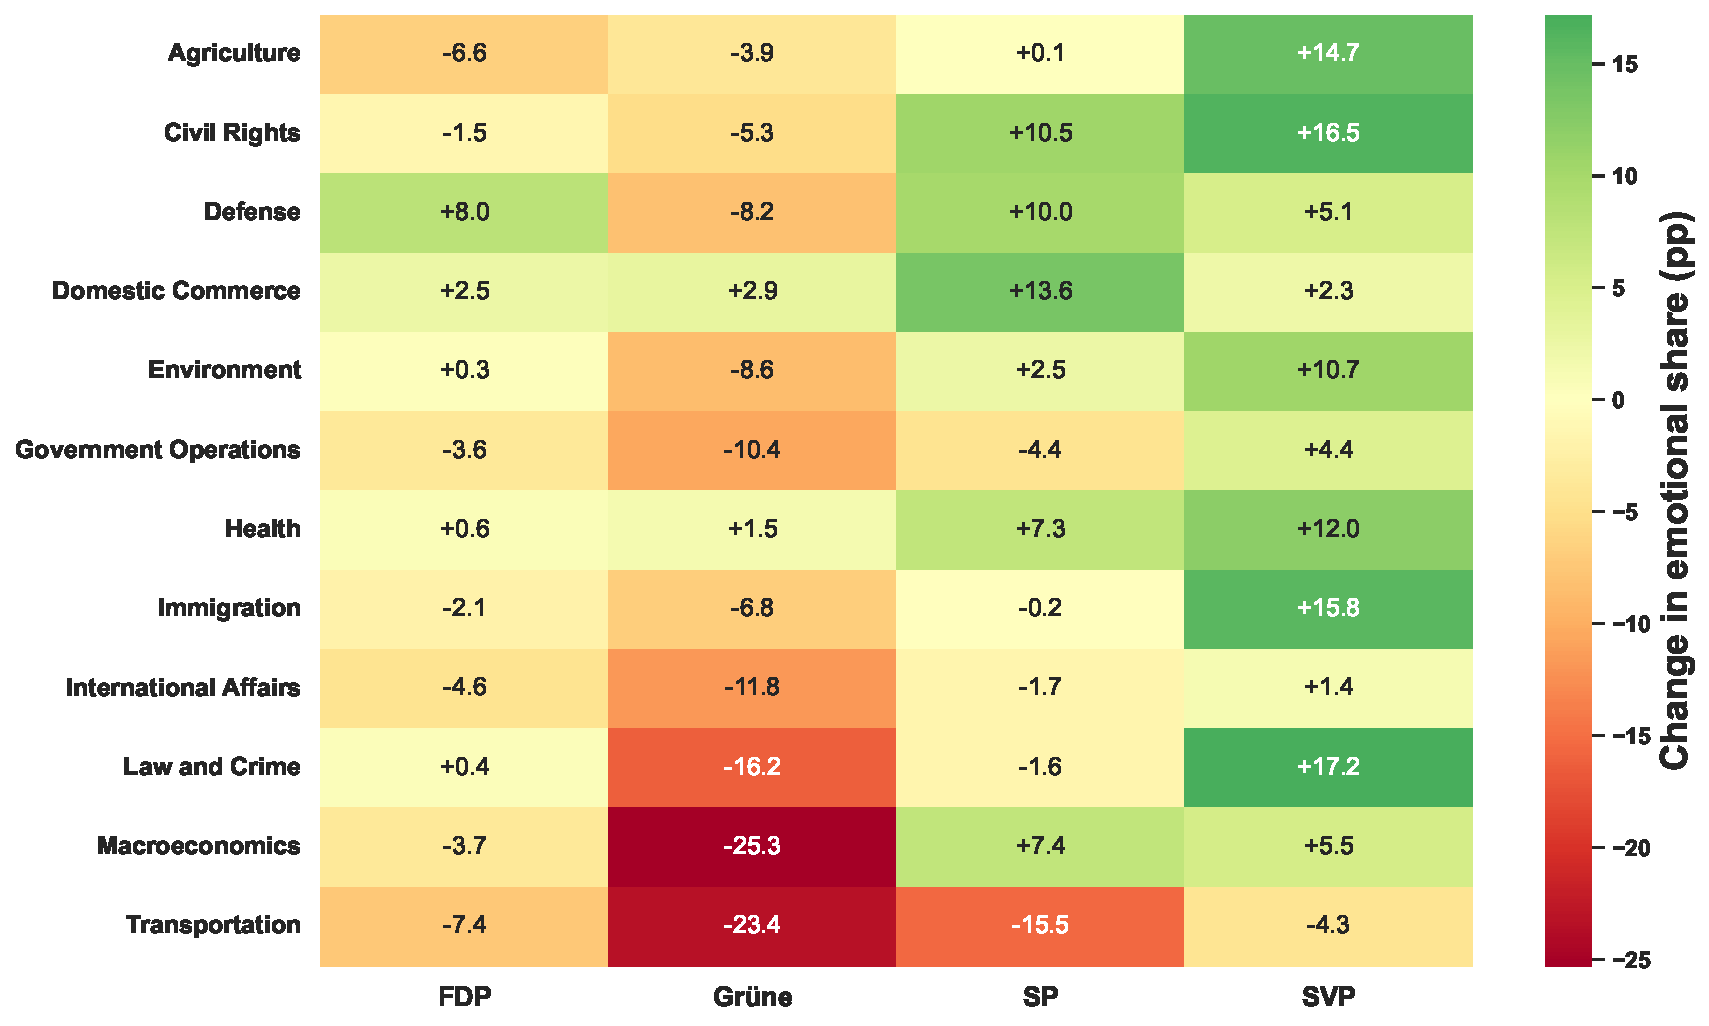
\includegraphics[width=0.88\textwidth,height=0.82\textheight,keepaspectratio]{fig_lt_defD_topic_shift_party.pdf}
    \end{frame}
\begin{frame}{Appendix --- Emotional-Rhetoric Shift by Topic and Party --- Ständerat}
    \centering
    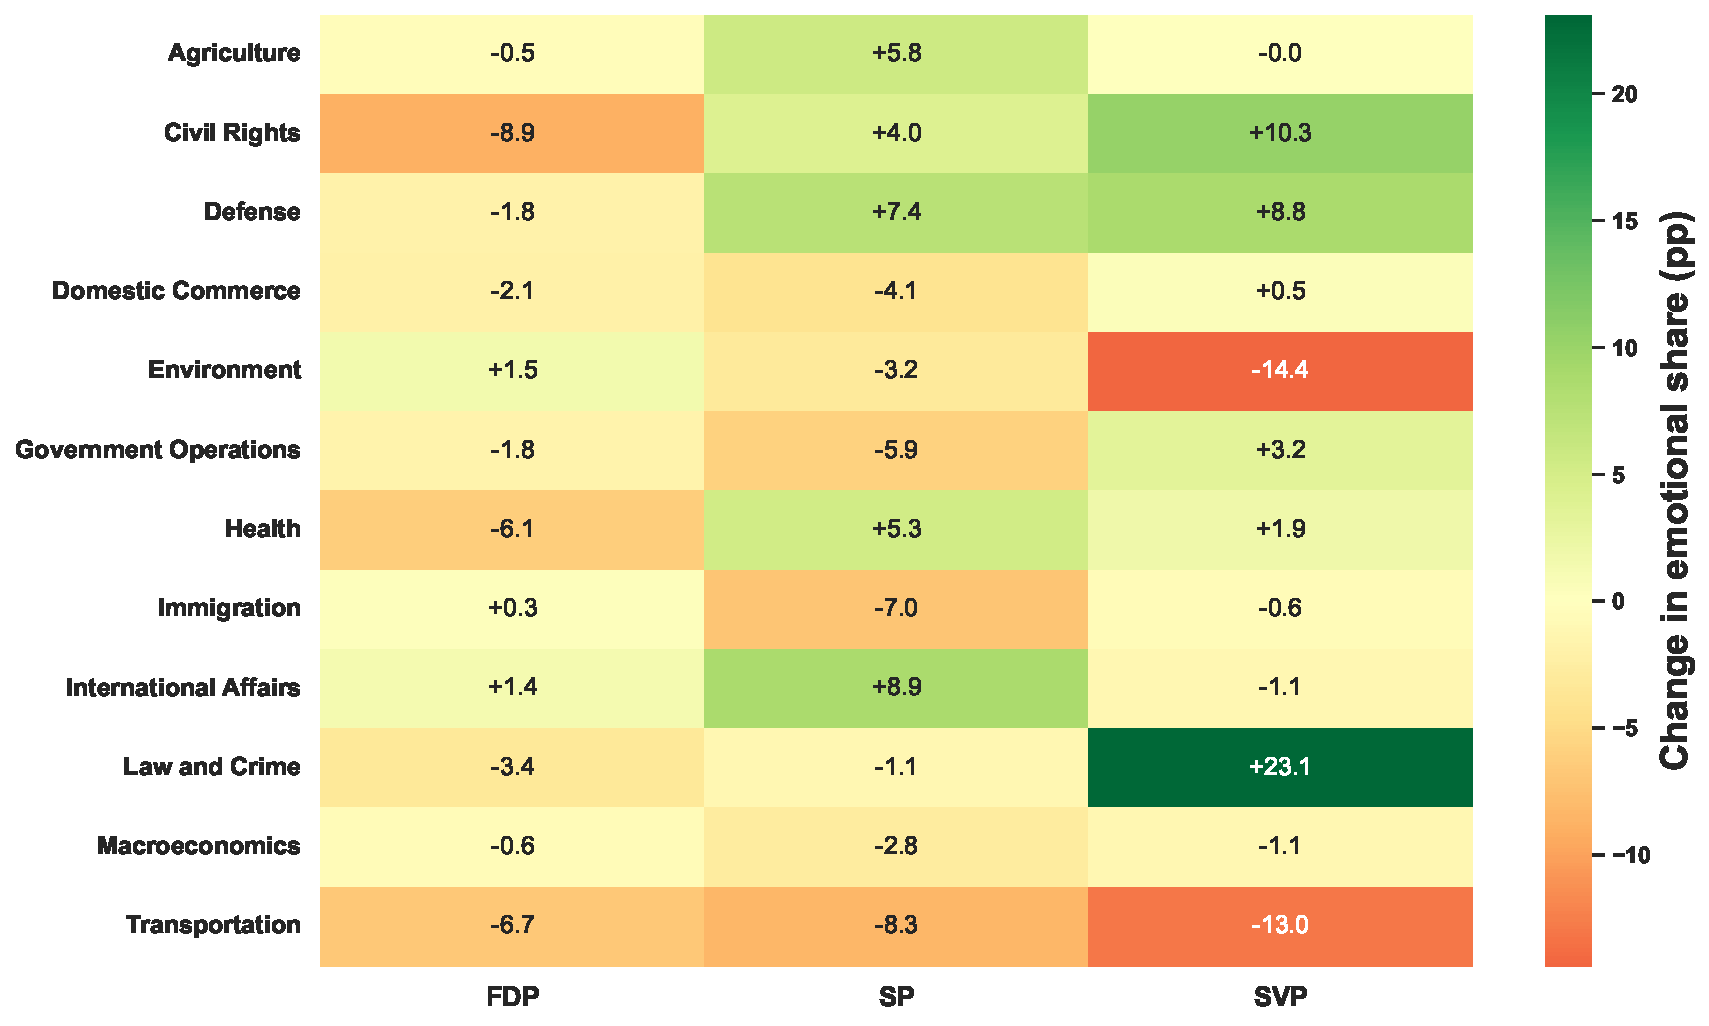
\includegraphics[width=0.88\textwidth,height=0.82\textheight,keepaspectratio]{staenderat_fig_lt_defD_topic_shift_party.pdf}
    \end{frame}
\begin{frame}{Appendix --- Anger by Party --- Nationalrat}
    \centering
    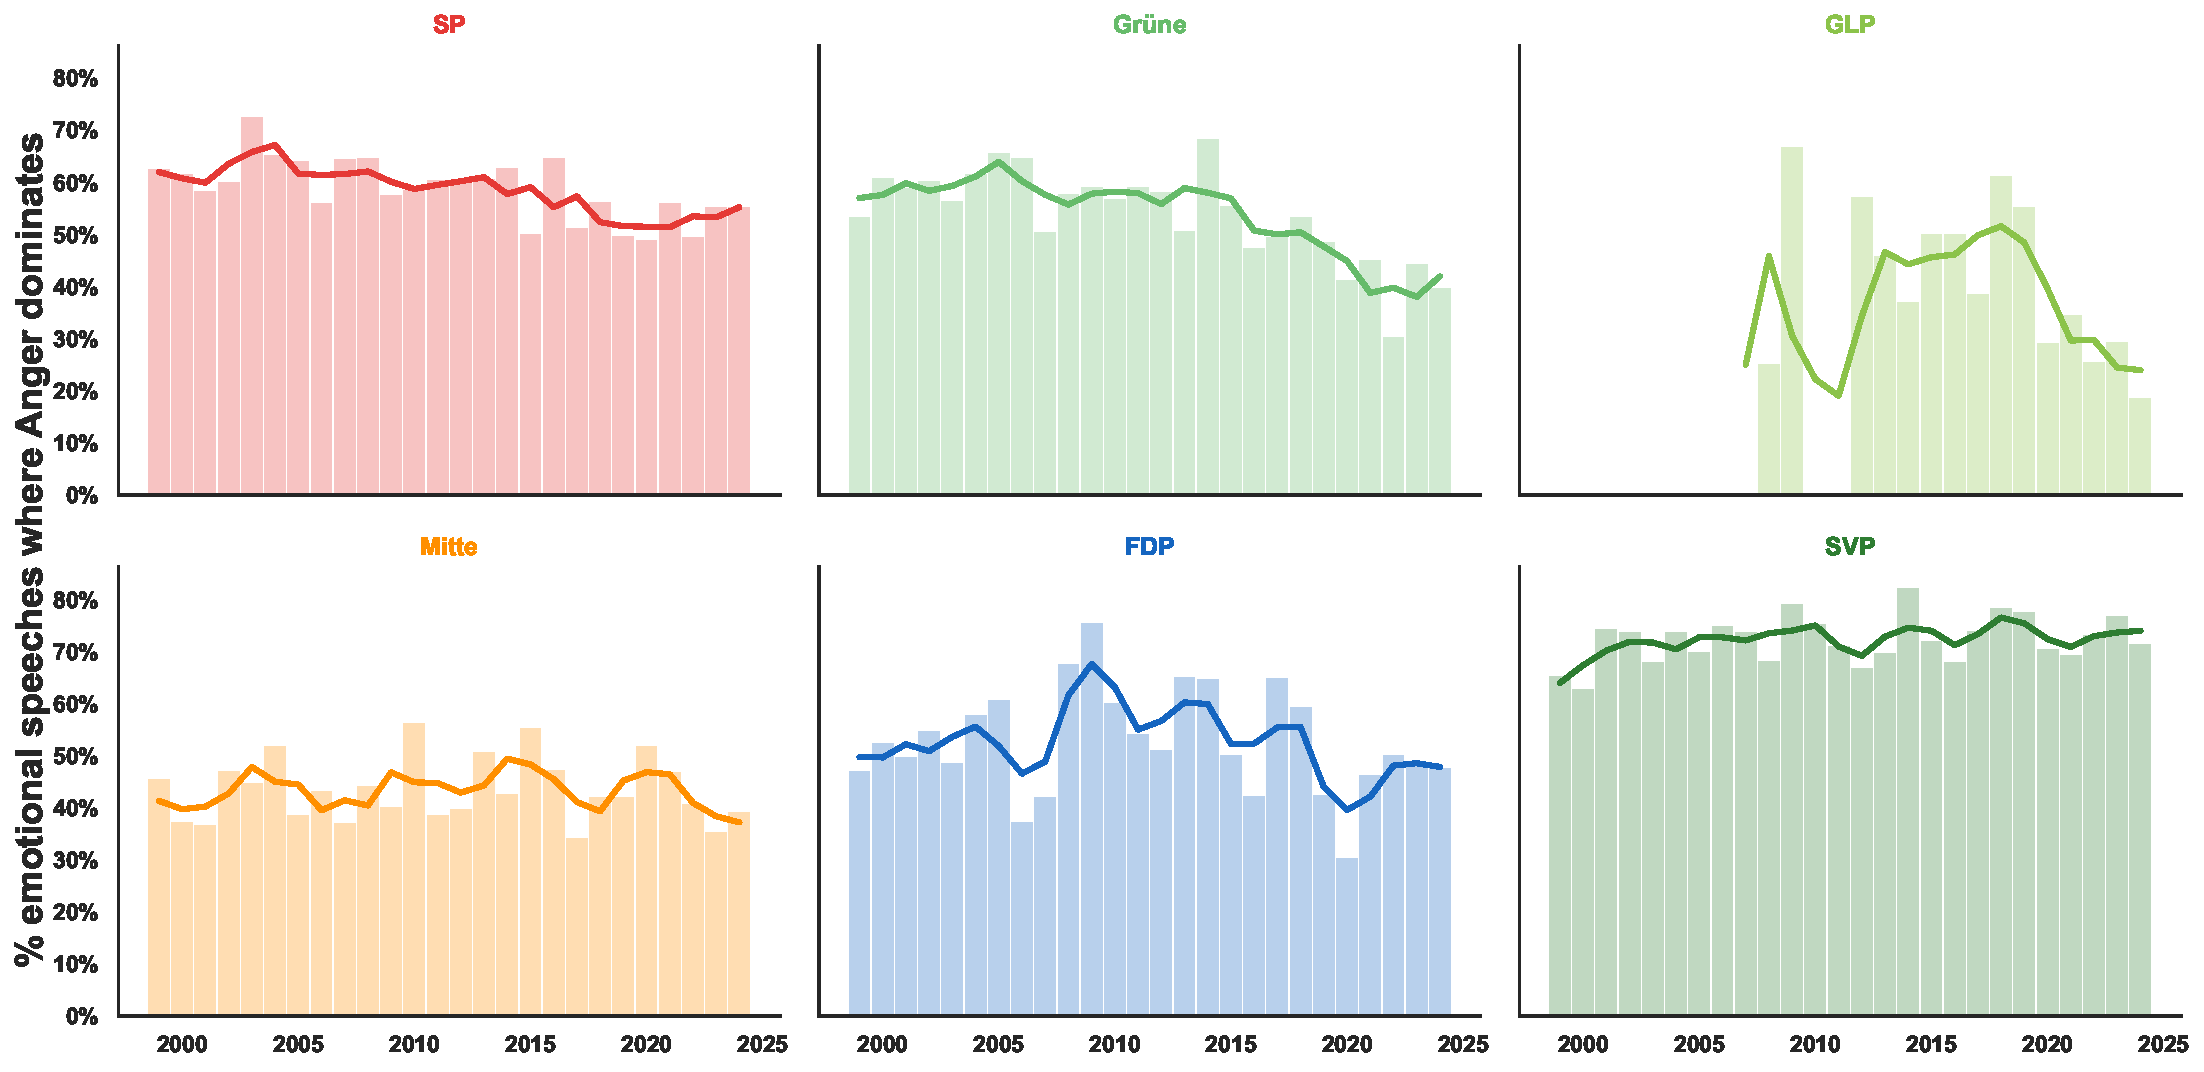
\includegraphics[width=0.88\textwidth,height=0.82\textheight,keepaspectratio]{fig_lt_llm_anger_share_party_facet.pdf}
    \end{frame}
\begin{frame}{Appendix --- Enthusiasm by Party --- Nationalrat}
    \centering
    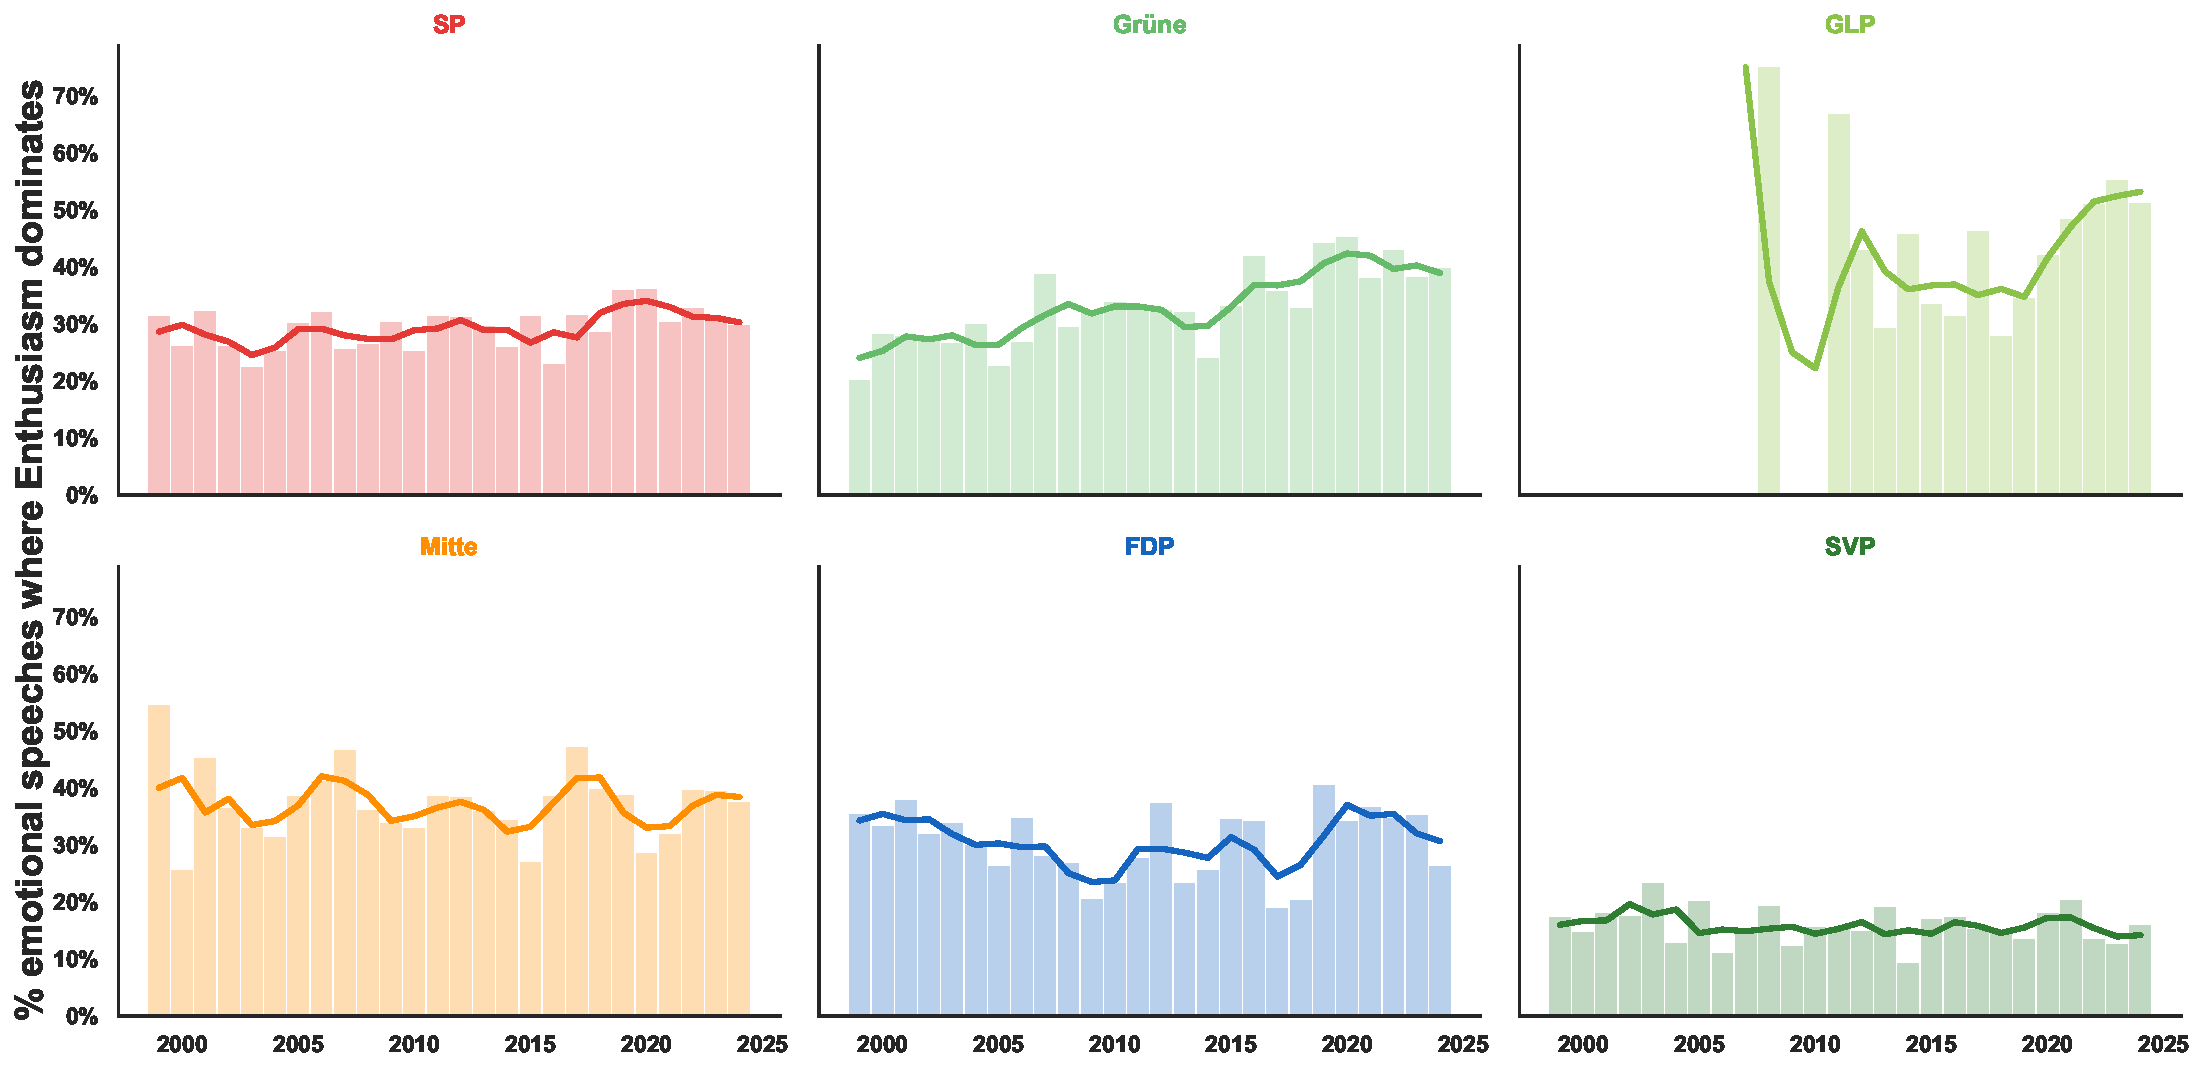
\includegraphics[width=0.88\textwidth,height=0.82\textheight,keepaspectratio]{fig_lt_llm_enthusiasm_share_party_facet.pdf}
    \end{frame}
\begin{frame}{Appendix --- Fear by Party --- Nationalrat}
    \centering
    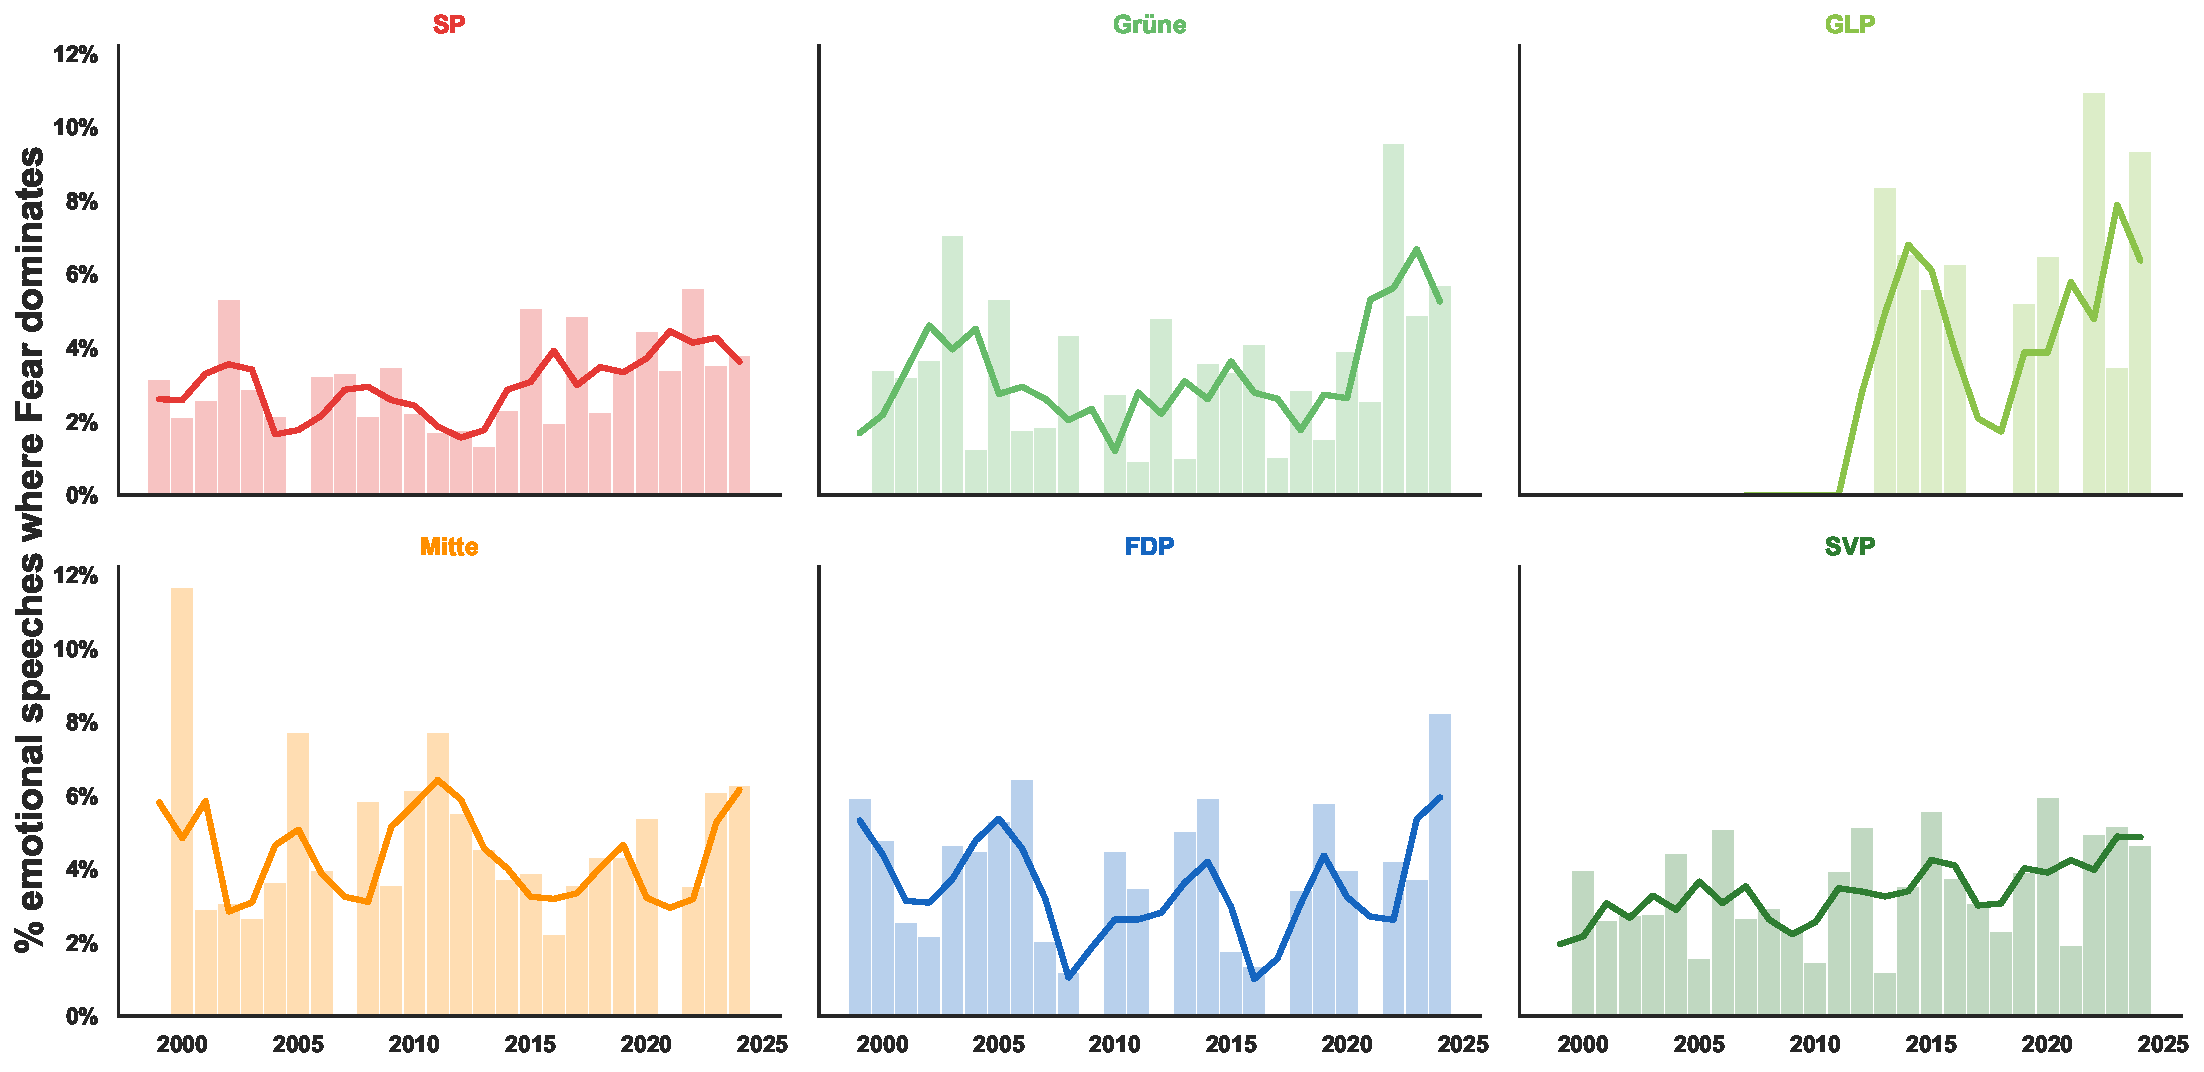
\includegraphics[width=0.88\textwidth,height=0.82\textheight,keepaspectratio]{fig_lt_llm_fear_share_party_facet.pdf}
    \end{frame}
\begin{frame}{Appendix --- Sadness by Party --- Nationalrat}
    \centering
    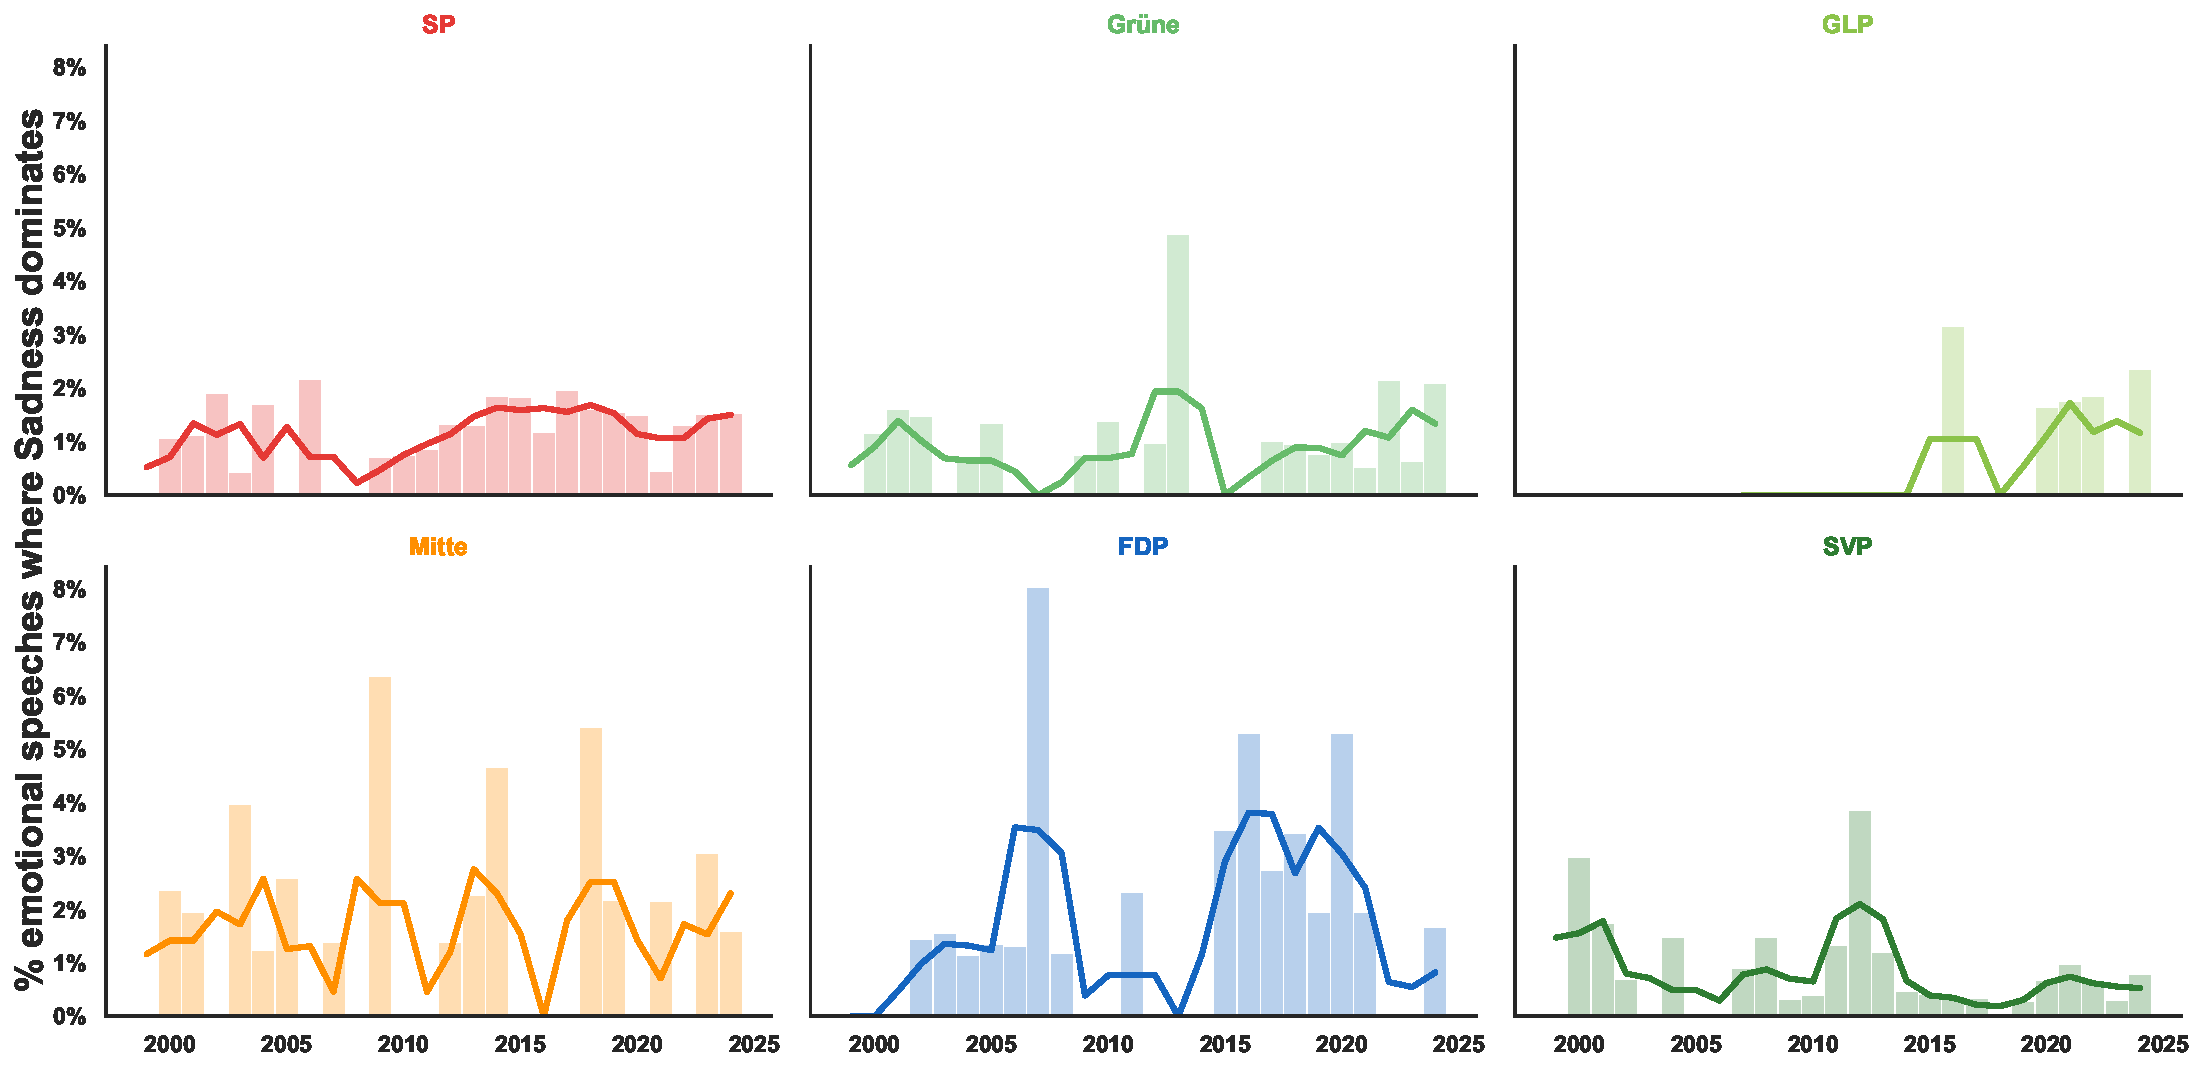
\includegraphics[width=0.88\textwidth,height=0.82\textheight,keepaspectratio]{fig_lt_llm_sadness_share_party_facet.pdf}
    \end{frame}
\begin{frame}{Appendix --- Disgust by Party --- Nationalrat}
    \centering
    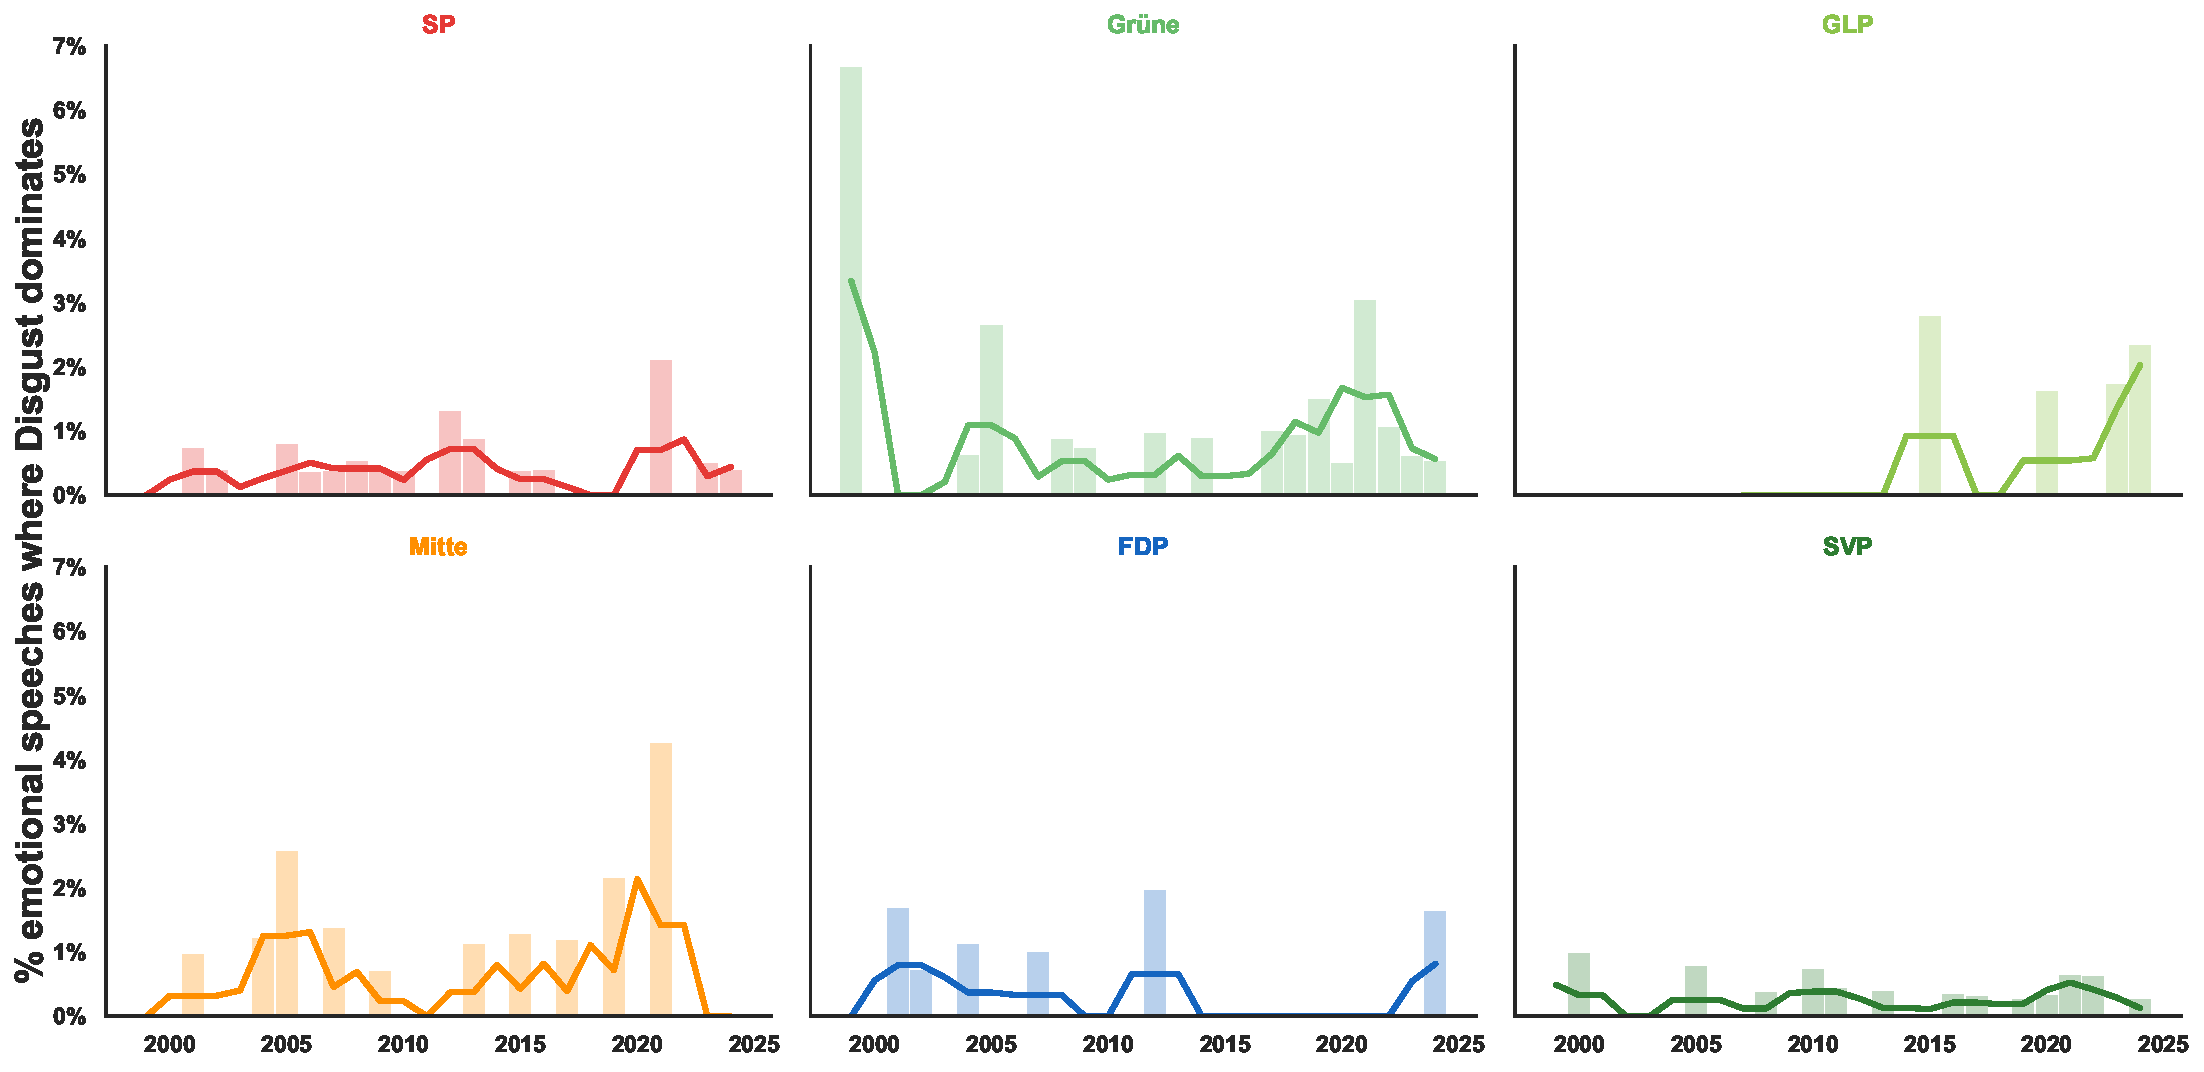
\includegraphics[width=0.88\textwidth,height=0.82\textheight,keepaspectratio]{fig_lt_llm_disgust_share_party_facet.pdf}
    \end{frame}
\begin{frame}{Appendix --- Anger by Party --- Ständerat}
    \centering
    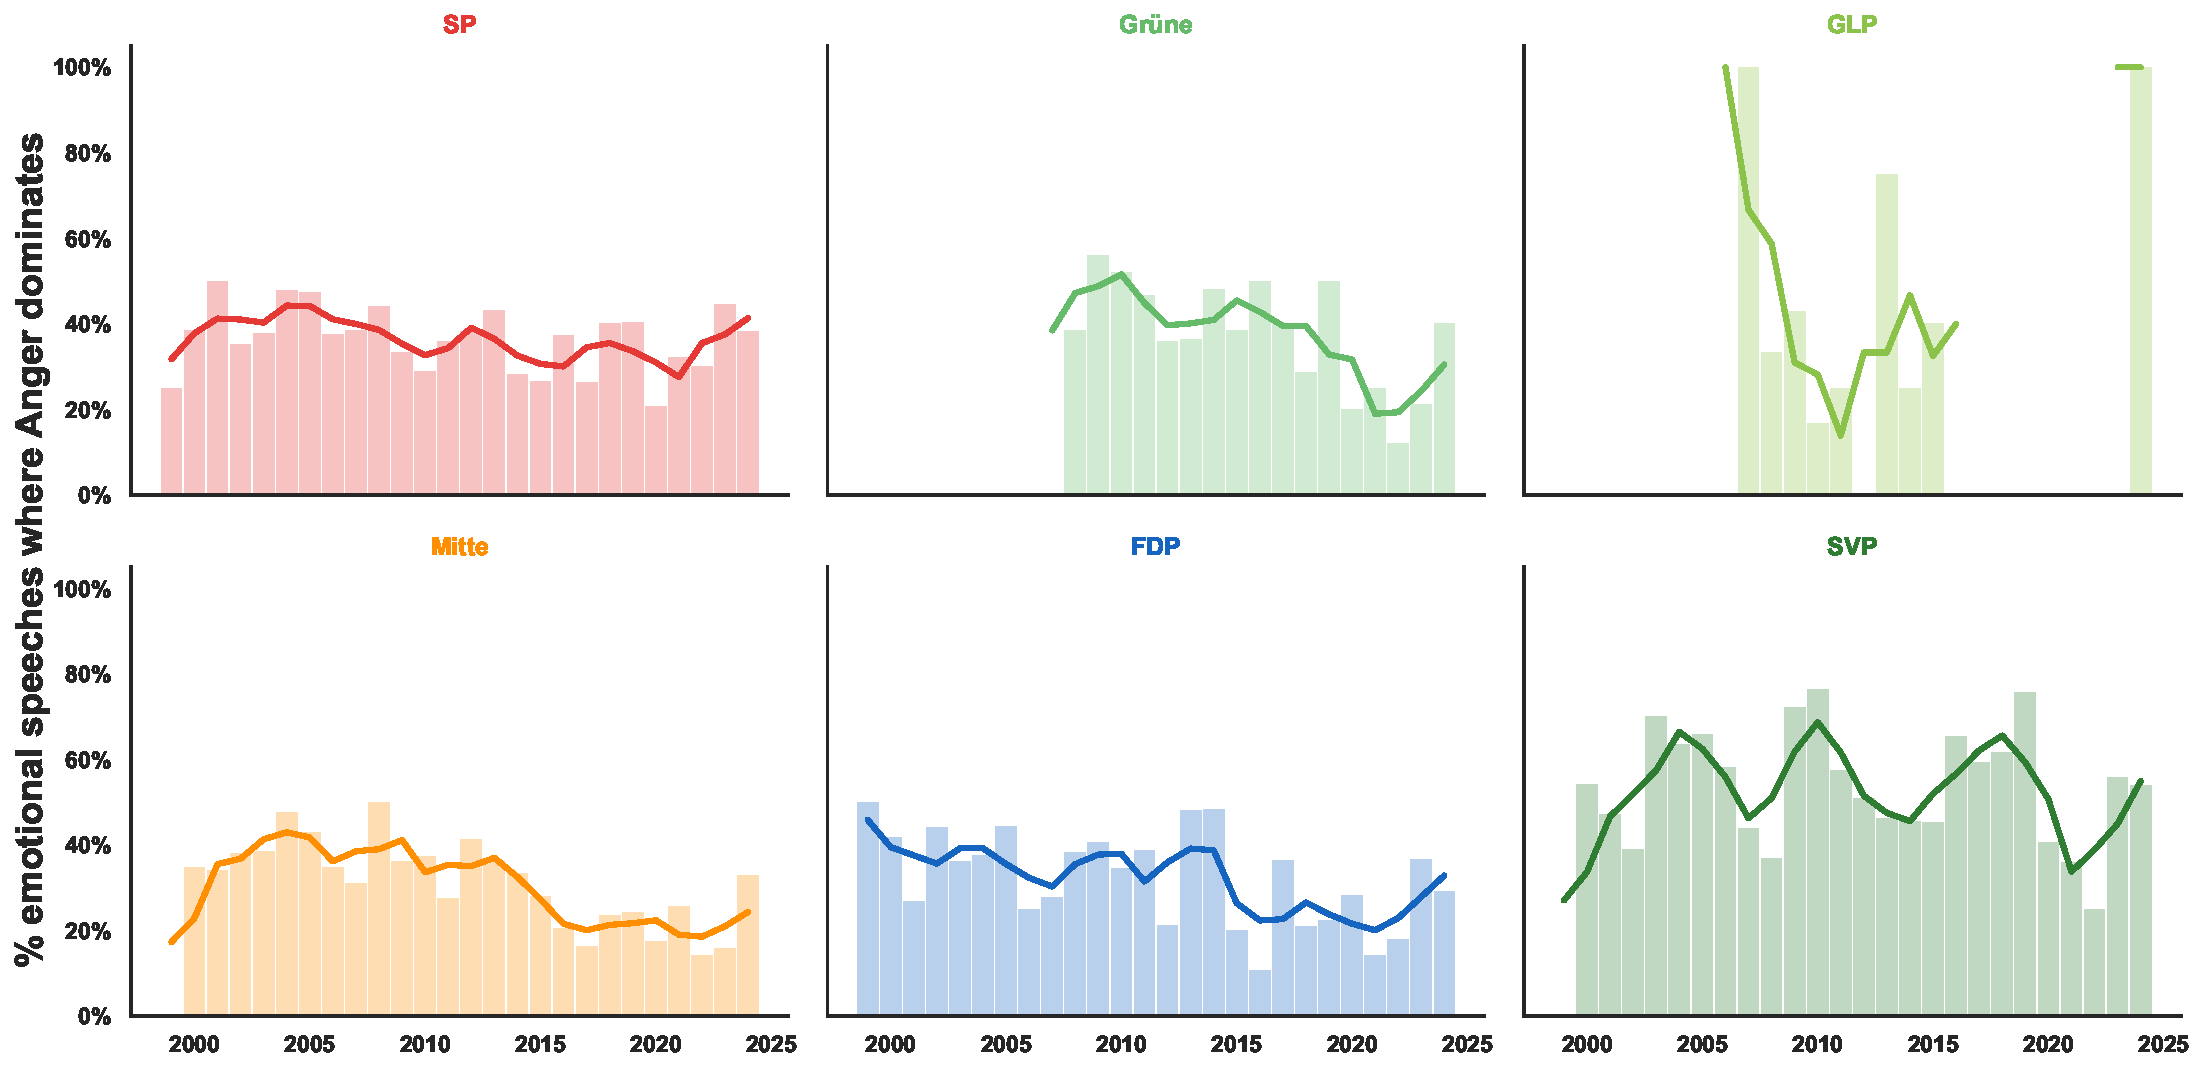
\includegraphics[width=0.88\textwidth,height=0.82\textheight,keepaspectratio]{staenderat_fig_lt_llm_anger_share_party_facet.pdf}
    \end{frame}
\begin{frame}{Appendix --- Enthusiasm by Party --- Ständerat}
    \centering
    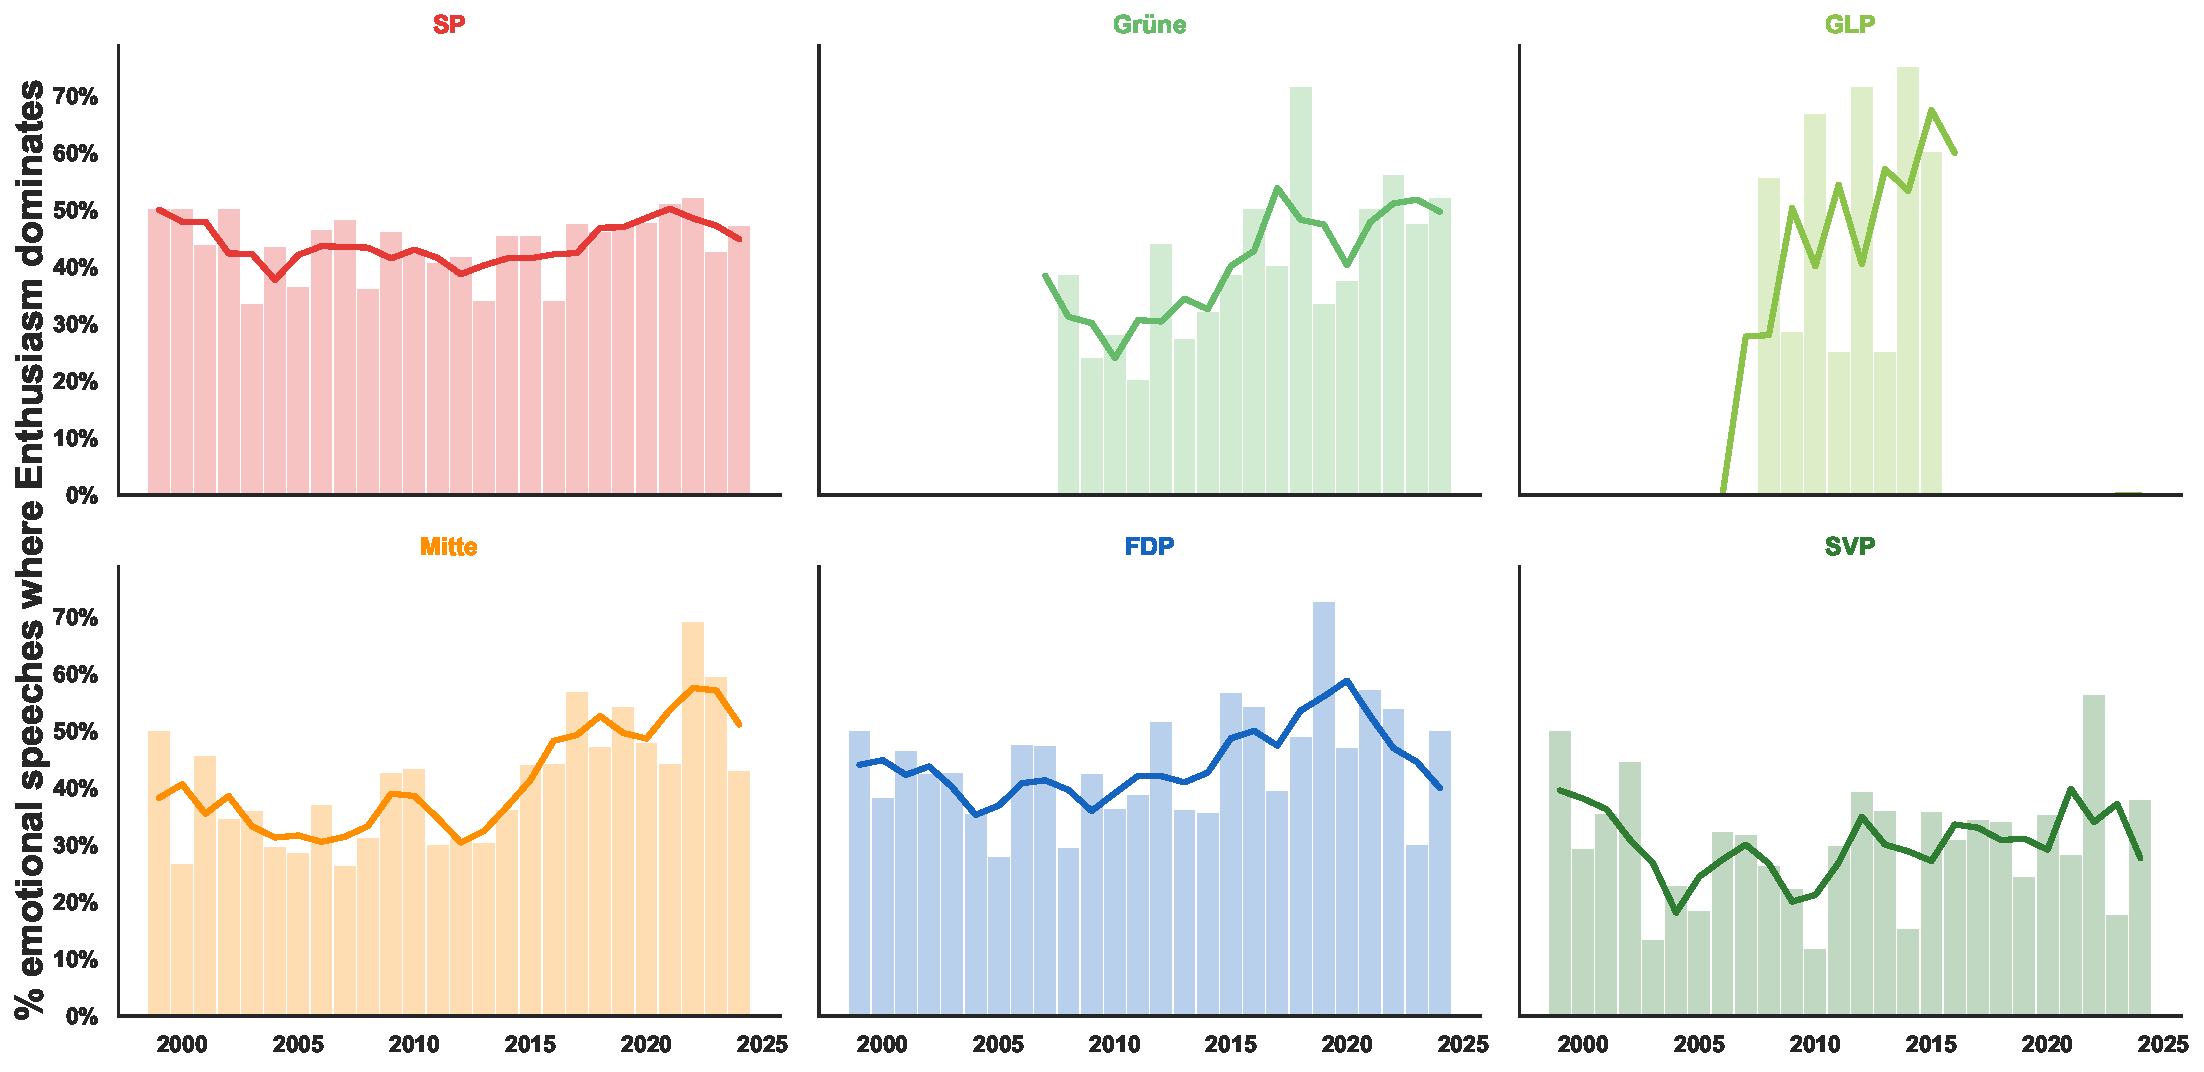
\includegraphics[width=0.88\textwidth,height=0.82\textheight,keepaspectratio]{staenderat_fig_lt_llm_enthusiasm_share_party_facet.pdf}
    \end{frame}
\begin{frame}{Appendix --- Fear by Party --- Ständerat}
    \centering
    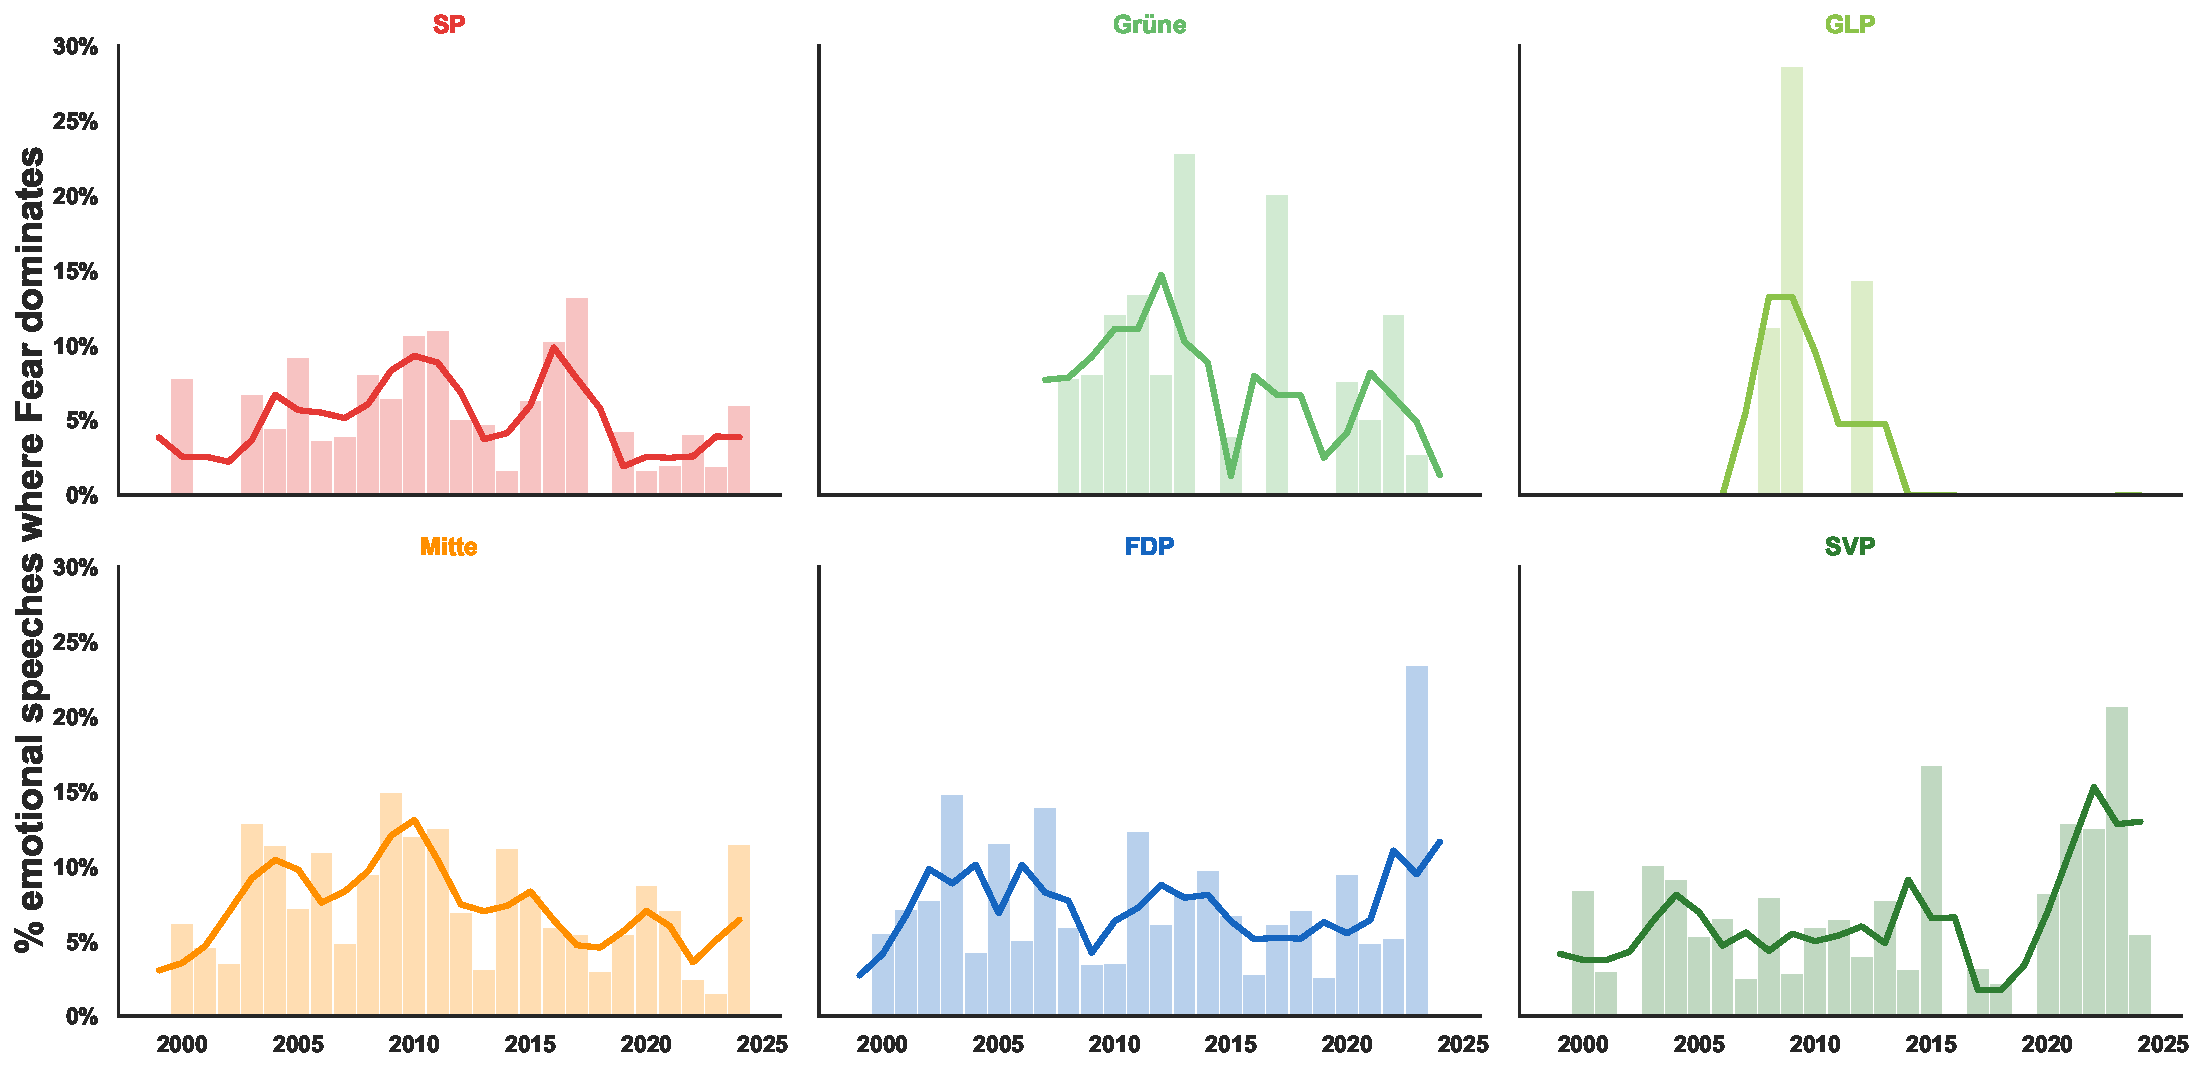
\includegraphics[width=0.88\textwidth,height=0.82\textheight,keepaspectratio]{staenderat_fig_lt_llm_fear_share_party_facet.pdf}
    \end{frame}
\begin{frame}{Appendix --- Sadness by Party --- Ständerat}
    \centering
    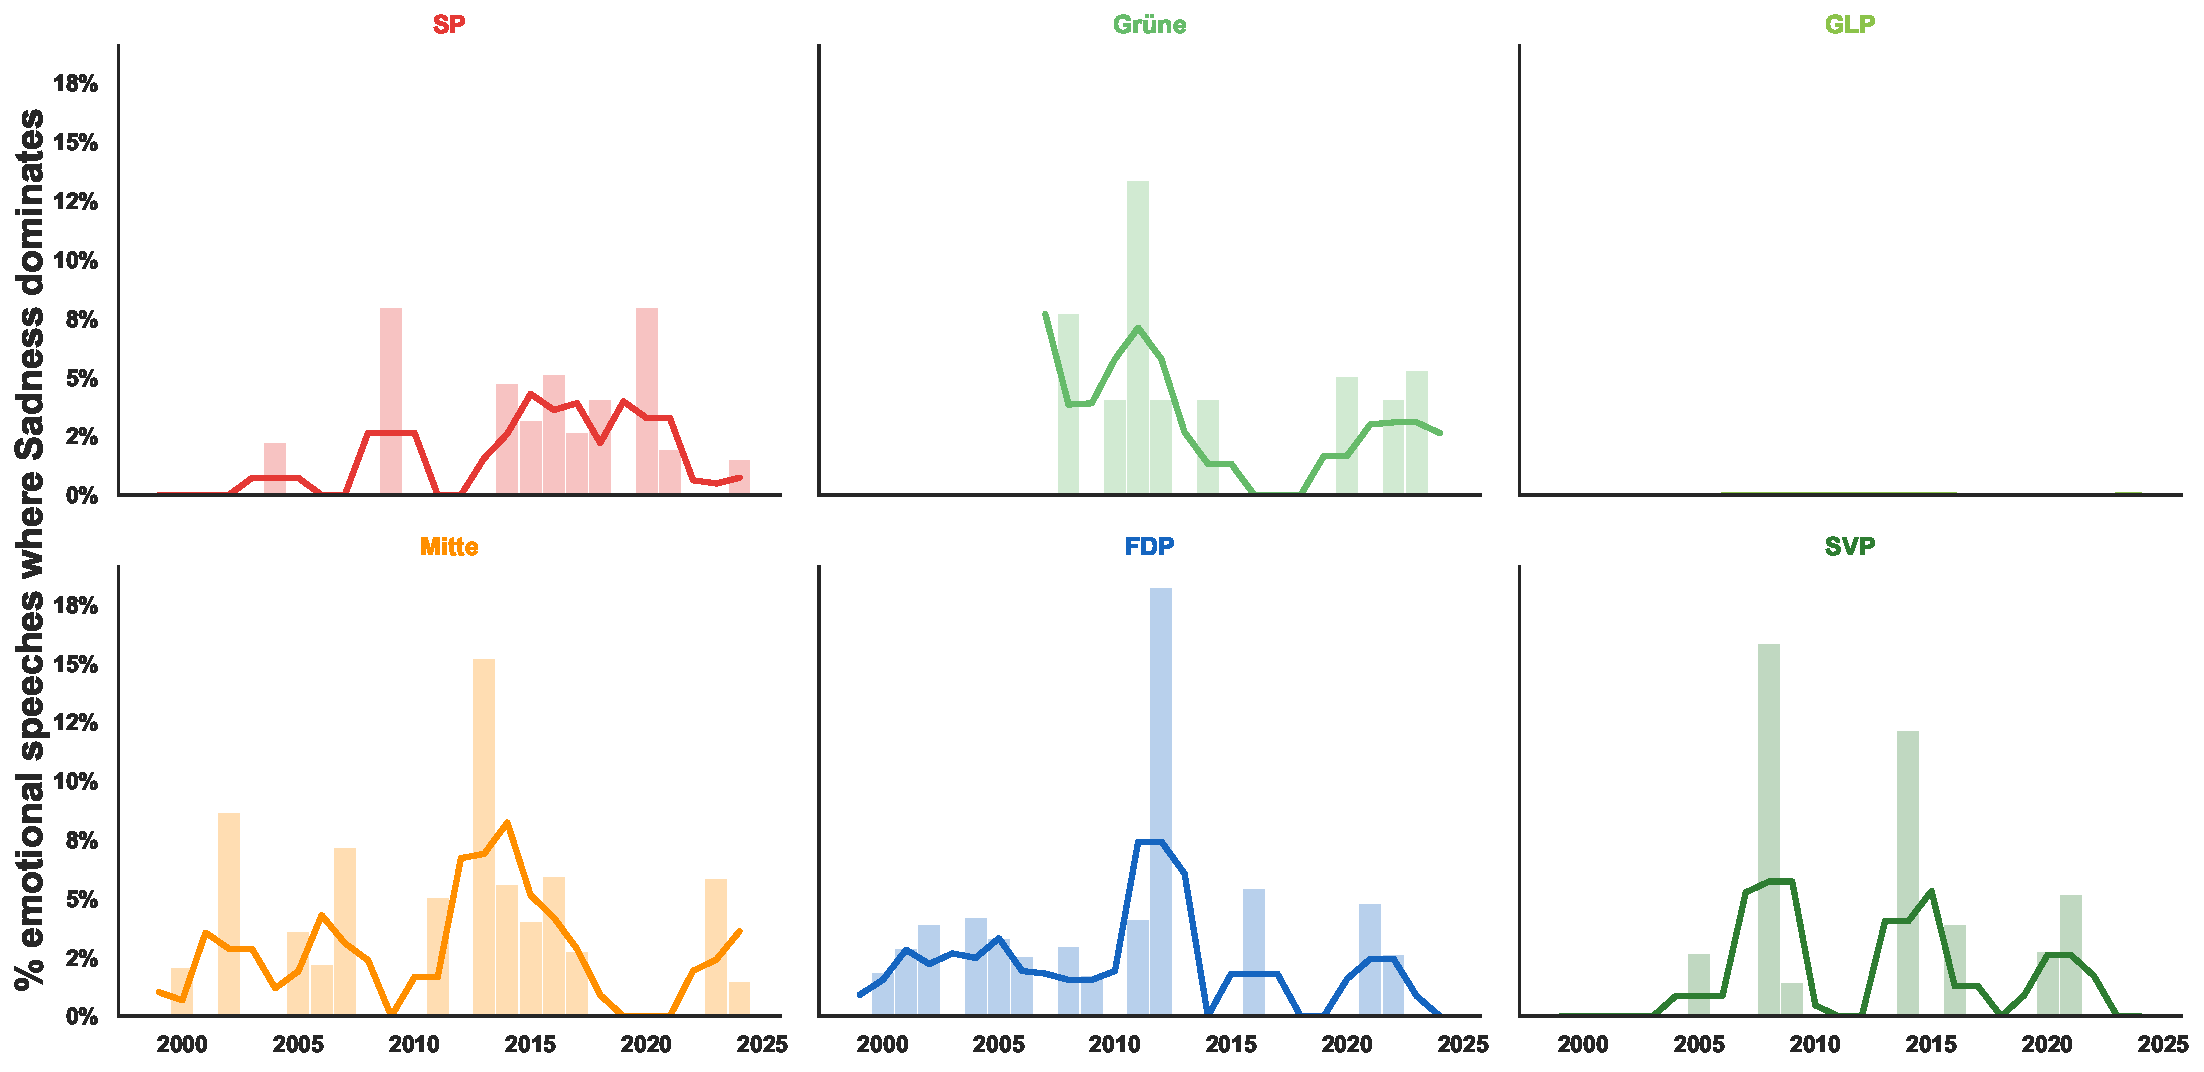
\includegraphics[width=0.88\textwidth,height=0.82\textheight,keepaspectratio]{staenderat_fig_lt_llm_sadness_share_party_facet.pdf}
    \end{frame}
\begin{frame}{Appendix --- Disgust by Party --- Ständerat}
    \centering
    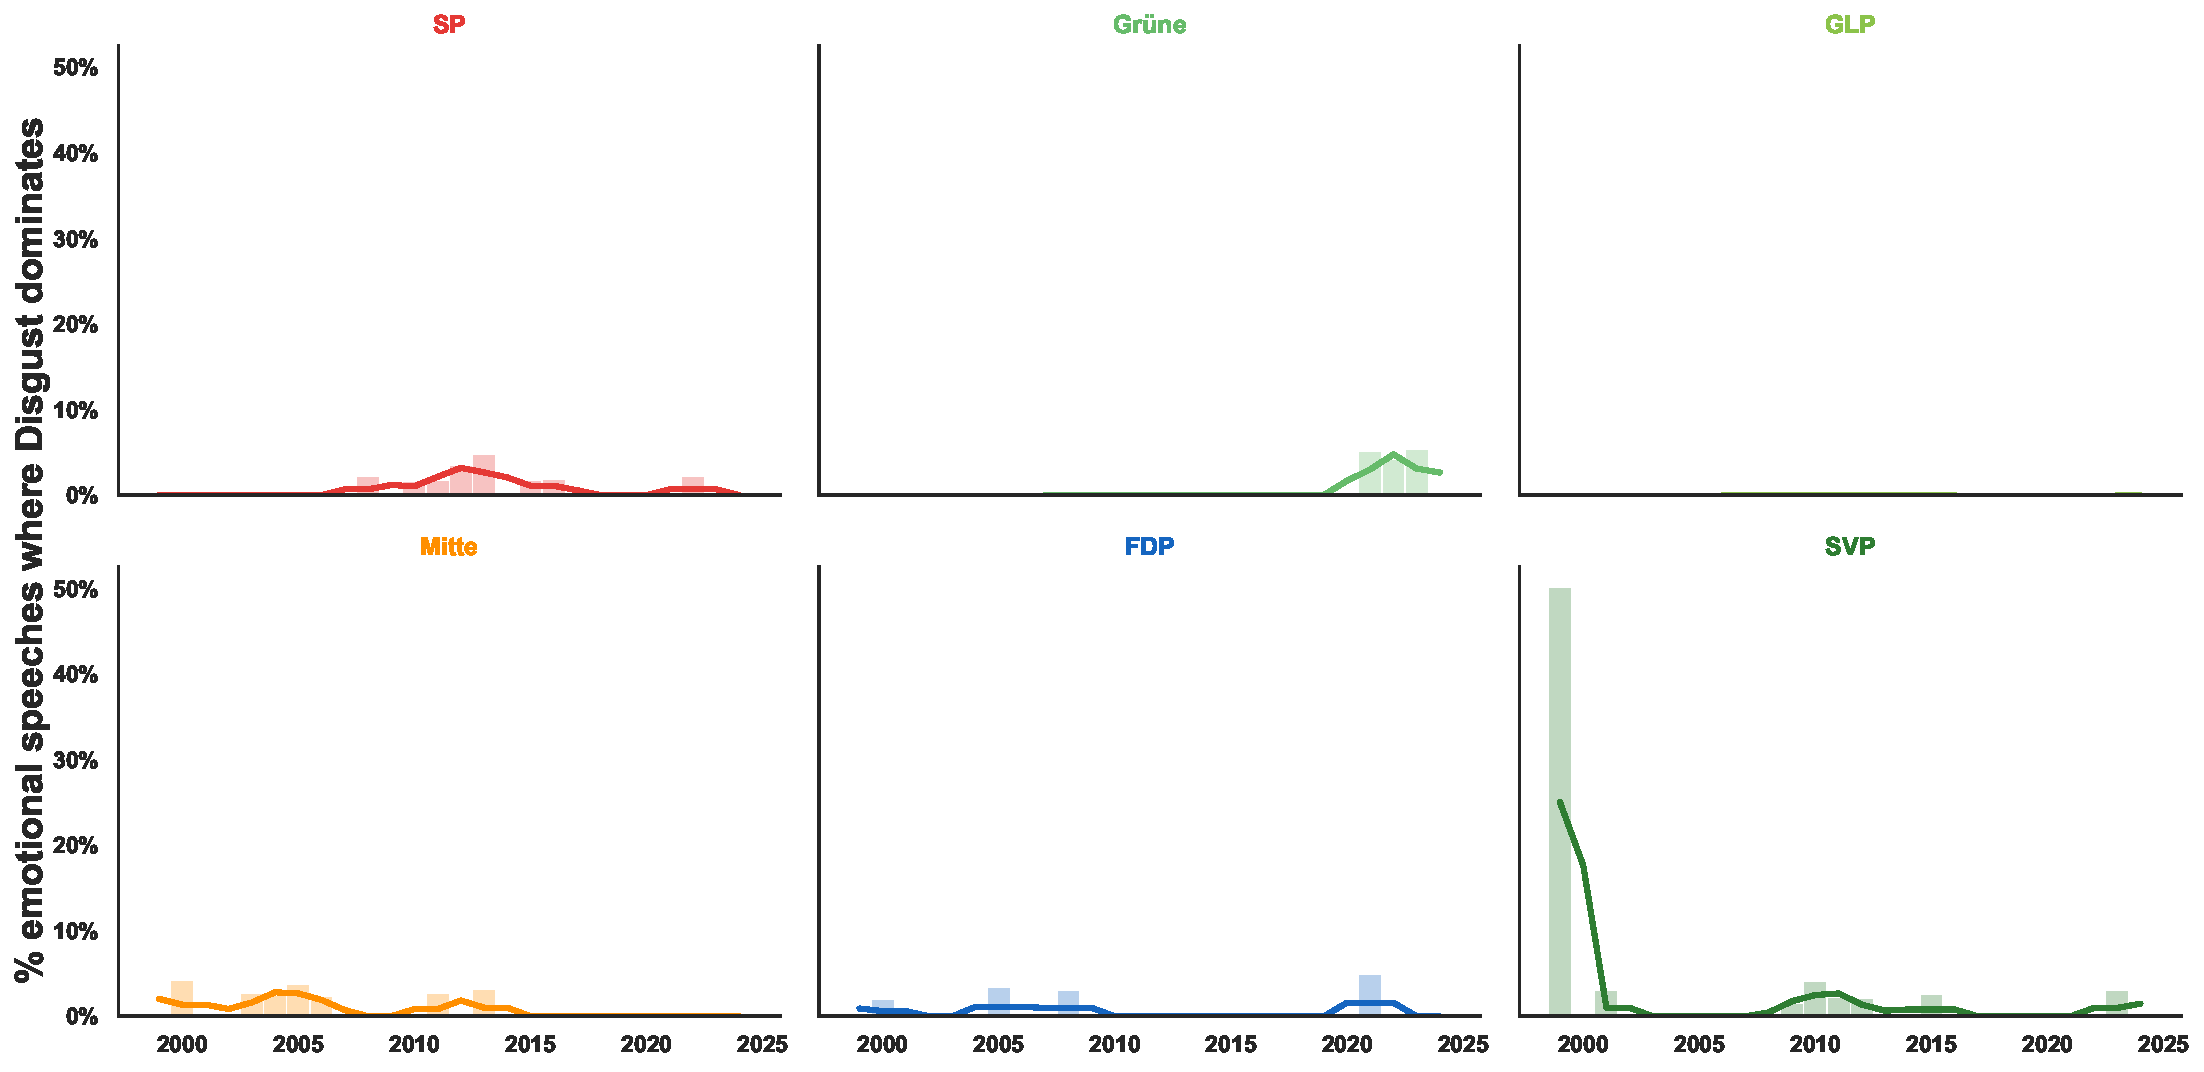
\includegraphics[width=0.88\textwidth,height=0.82\textheight,keepaspectratio]{staenderat_fig_lt_llm_disgust_share_party_facet.pdf}
    \end{frame}

\end{document}
